%\documentclass[12pt]{report}
\documentclass[a4paper,12pt,oneside]{book}
%\usepackage[a4paper, margin=2cm, footskip=15pt]{geometry}
\usepackage[a4paper,top=3.5cm,left=3cm,right=3cm,bottom=2.5cm]{geometry}
\usepackage{times} %pacote da fonte Times New Roman
\usepackage[utf8]{inputenc}
%\usepackage[T1]{fontenc}
\usepackage[export]{adjustbox}
\usepackage{caption}
\usepackage{subcaption}
\usepackage{setspace}
\usepackage{indentfirst}
\usepackage{float}
\usepackage{amsmath}
\usepackage{appendix}
%\usepackage{pgfplots}
% \usepackage{unicode-math}
\newcommand\mathplus{+}
% \usepackage{subfigure}
% \usepackage{algorithm}
% \usepackage[ruled,vlined,lined,linesnumbered,spanish, onelanguage]{algorithm2e}
\usepackage[ruled,vlined,lined,linesnumbered,portuguese, onelanguage]{algorithm2e}
% \usepackage{algorithmic}
\usepackage{algpseudocode}
\renewcommand{\baselinestretch}{1.3}
\usepackage[backend=bibtex, style=numeric, sorting=none]{biblatex}
\addbibresource{sample.bib}
%\renewcommand{\listalgorithm}{Lista de Algoritmos}%
%\renewcommand{\algorithm}{Algoritmo}%
%\renewcommand{\algocf@typo}{}%
%\renewcommand{\@algocf@procname}{Procedimento}
%\renewcommand{\@algocf@funcname}{Fun\c{c}\~{a}o}
\usepackage[scr=rsfs]{mathalpha}
\DeclareMathOperator{\sinc}{sinc}
\DeclareMathOperator{\rect}{rect}
\DeclareMathOperator{\atantwo}{atan2}

\usepackage{hyperref}
\hypersetup{colorlinks=false, pdftitle={Tese}}
% \usepackage[backend=biber]{biblatex}
% \addbibresource{sample.bib}
\renewcommand\appendixname{Apêndice}
\renewcommand\appendixpagename{Apêndices}

\usepackage{alphalph}
\renewcommand*{\thesubfigure}{%
\alphalph{\value{subfigure}}%
}%
\hyphenation{mo-de-lo}
\hyphenation{par-ti-cu-lar}
\hyphenation{a-li-nha-dos}
\hyphenation{ex-pe-ri-men-to}
\hyphenation{de-ta-lhes}
\hyphenation{in-te-ra-gem}
\hyphenation{ou-tros}
\hyphenation{ge-ra-dos}
\hyphenation{a-na-li-sar}
\hyphenation{di-fe-ren-tes}
\hyphenation{va-lo-res}
\hyphenation{es-co-lhi-do}
\hyphenation{tem-pe-ra-tu-ra}
\hyphenation{cor-res-pon-de}
\hyphenation{li-te-ra-tu-ra}
\hyphenation{in-di-vi-du-al}

\usepackage[final]{pdfpages}




\begin{document}
%\pagenumbering{roman}
%\pagestyle{plain}
\captionsetup[figure]{name={Figura}}
\renewcommand*\contentsname{Sumário}
\renewcommand{\listfigurename}{Lista de figuras}
\renewcommand{\listoftables}{Tabelas}
\renewcommand{\listofalgorithms}{Lista de algoritmos}
\makeatletter
\renewcommand{\@chapapp}{Capítulo}
\makeatother
\addtocounter{page}{0}


\thispagestyle{empty}
%\pagenumbering{arabic}
\begin{center}

%%%%%%%%%%%%%%%%%%%%%%%%%%%%%%%%%%%%%%%%%%%%%%%%%%%%%%%%%%%%%%%%%%%%%%%%%%%%%%%%%%%%%    
%\Título da Tese \ Thesis title
	{\fontsize{16}{16} \selectfont Universidade de S\~ao Paulo \\}
	\vspace{0.1cm}
	{\fontsize{16}{16} \selectfont Instituto de F\'{i}sica}
    \vspace{2.2cm}

	{\fontsize{22}{22}\selectfont Estudo da reação de breakup $^4$He($^{17}$F,$^{16}$O+$p$)$^4$He usando o alvo ativo pAT-TPC: uma abordagem usando técnicas de Machine Learning\par}
    \vspace{2cm}

%%%%%%%%%%%%%%%%%%%%%%%%%%%%%%%%%%%%%%%%%%%%%%%%%%%%%%%%%%%%%%%%%%%%%%%%%%%%%%%%%%%%%    
%\Nome do Autor \ Author's name

    {\fontsize{18}{18}\selectfont Guilherme Ferrari Fortino\par}

    \vspace{1.4cm}

\end{center}

%%%%%%%%%%%%%%%%%%%%%%%%%%%%%%%%%%%%%%%%%%%%%%%%%%%%%%%%%%%%%%%%%%%%%%%%%%%%%%%%%%%%%%    
%\Orientador e coorientador (se existir) \ Supervisor and co-supervisor (if there is one)
\leftskip 6cm
\begin{flushright}	
\leftskip 6cm
Orientador: Prof. Dr.  Valdir Guimar\~{a}es\hfill{ \hskip 5cm  } 
\leftskip 6cm
\newline
    %Se não houve coorientador, comente a linha abaixo \ If there is no co-advisor, comment line below
Coorientador: Dr. Juan Carlos Zamora Cardona\hfill{ \hskip 4cm  }
\end{flushright}	

\vspace{0.6cm}    

%%%%%%%%%%%%%%%%%%%%%%%%%%%%%%%%%%%%%%%%%%%%%%%%%%%%%%%%%%%%%%%%%%%%%%%%%%%%%%%%%%%%%    
% Grau Acadêmico \ Degree

\par
\leftskip 6cm
\noindent {Disserta\c{c}\~{a}o de mestrado apresentada ao Instituto de F\'{i}sica da Universidade de S\~{a}o Paulo, como requisito parcial para a obten\c{c}\~{a}o do t\'{i}tulo de Mestre(a) em Ci\^{e}ncias.}
\par
\leftskip 0cm
\vskip 2cm

%%%%%%%%%%%%%%%%%%%%%%%%%%%%%%%%%%%%%%%%%%%%%%%%%%%%%%%%%%%%%%%%%%%%%%%%%%%%%%%%%%%%    
% Banca Examinadora -- Primeiro nome é do presidente ou do presidente da banca \ Examining committee -- The first name must be the supervisor's name or the examination committee president's name.

\noindent Banca Examinadora: \\
\noindent Dr. Juan Carlos Zamora Cardona - Coorientador (IFUSP/MSU) \\
Prof. Dr. Mario Olimpio de Menezes (IPEN) \\
Prof. Dr. Brett Vern Carlson (ITA) \\
\vspace{1.8cm}


%%%%%%%%%%%%%%%%%%%%%%%%%%%%%%%%%%%%%%%%%%%%%%%%%%%%%%%%%%%%%%%%%%%%%%%%%%%%%%%%%%%%    
%Data \ Date
\begin{center}
    {S\~ao Paulo \\  2022}
\end{center}%\centering
%\newpage
\newpage

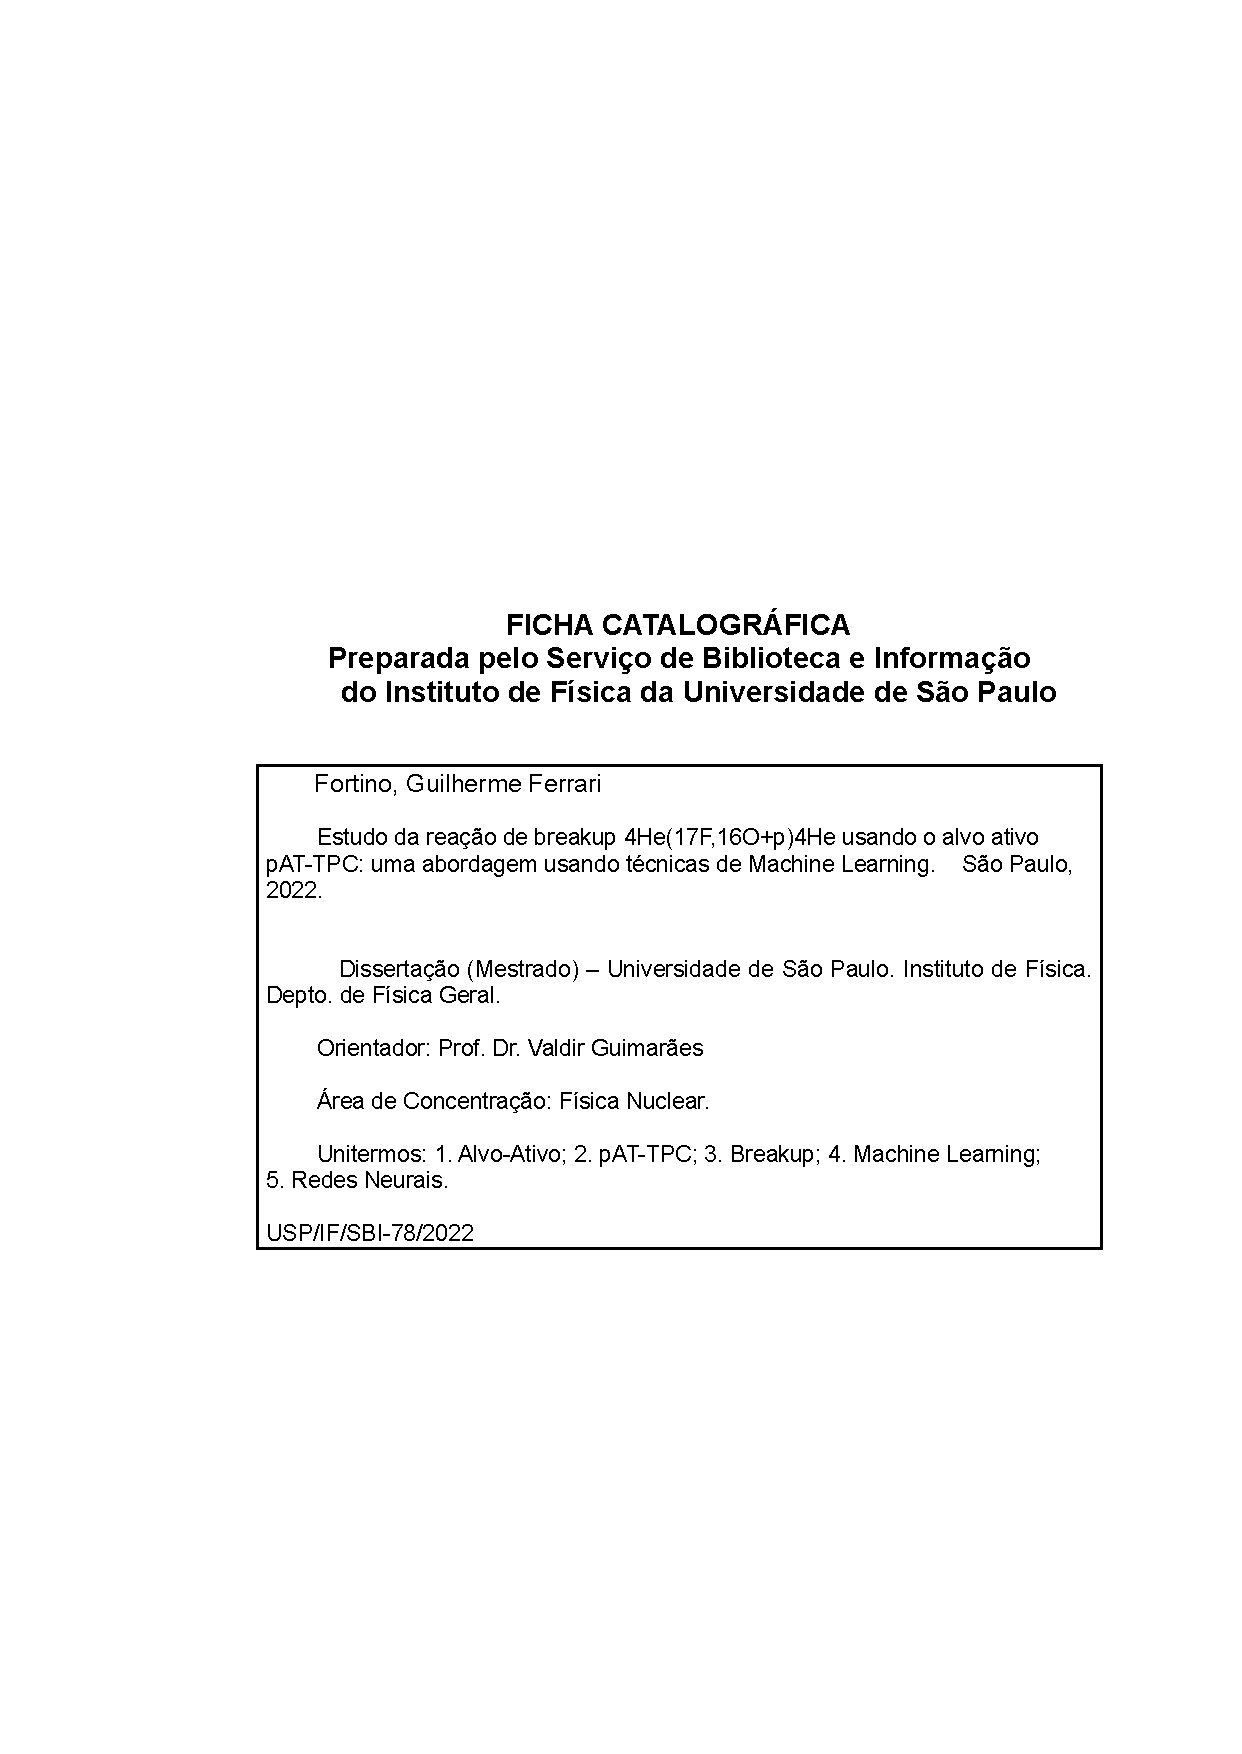
\includepdf[pages=-]{fc78-2022.doc.pdf}
\newpage
\thispagestyle{empty}
\begin{center}

%%%%%%%%%%%%%%%%%%%%%%%%%%%%%%%%%%%%%%%%%%%%%%%%%%%%%%%%%%%%%%%%%%%%%%%%%%%%%%%%%%%%%    
%\Título da Tese \ Thesis title
	{\fontsize{16}{16} \selectfont University of São Paulo \\}
	\vspace{0.1cm}
	{\fontsize{16}{16} \selectfont Physics Institute}
    \vspace{2.2cm}

	{\fontsize{22}{22}\selectfont Breakup reaction study $^4$He($^{17}$F,$^{16}$O+$p$)$^4$He using the pAT-TPC active target: an approach using Machine Learning techniques\par}
    \vspace{2cm}

%%%%%%%%%%%%%%%%%%%%%%%%%%%%%%%%%%%%%%%%%%%%%%%%%%%%%%%%%%%%%%%%%%%%%%%%%%%%%%%%%%%%%    
%\Nome do Autor \ Author's name

    {\fontsize{18}{18}\selectfont Guilherme Ferrari Fortino\par}

    \vspace{1.4cm}

\end{center}

%%%%%%%%%%%%%%%%%%%%%%%%%%%%%%%%%%%%%%%%%%%%%%%%%%%%%%%%%%%%%%%%%%%%%%%%%%%%%%%%%%%%%%    
%\Orientador e coorientador (se existir) \ Supervisor and co-supervisor (if there is one)
\leftskip 6cm
\begin{flushright}	
\leftskip 6cm
Advisor: Prof. Dr.  Valdir Guimarães\hfill{ \hskip 5cm  } 
\leftskip 6cm
\newline
    %Se não houve coorientador, comente a linha abaixo \ If there is no co-advisor, comment line below
Co-advisor: Dr. Juan Carlos Zamora Cardona\hfill{ \hskip 4cm  }
\end{flushright}	

\vspace{0.6cm}    

%%%%%%%%%%%%%%%%%%%%%%%%%%%%%%%%%%%%%%%%%%%%%%%%%%%%%%%%%%%%%%%%%%%%%%%%%%%%%%%%%%%%%    
% Grau Acadêmico \ Degree

\par
\leftskip 6cm
\noindent {Dissertation submitted to the Physics Institute of the University of São Paulo in partial fulfillment of the requirements for the degree of Master of Science.}
\par
\leftskip 0cm
\vskip 2cm

%%%%%%%%%%%%%%%%%%%%%%%%%%%%%%%%%%%%%%%%%%%%%%%%%%%%%%%%%%%%%%%%%%%%%%%%%%%%%%%%%%%%    
% Banca Examinadora -- Primeiro nome é do presidente ou do presidente da banca \ Examining committee -- The first name must be the supervisor's name or the examination committee president's name.

\noindent Examining Committee: \\
\noindent Prof. Dr. Juan Carlos Zamora Cardona - Co-advisor (IFUSP/MSU) \\
Prof. Dr. Mario Olimpio de Menezes (IPEN) \\
Prof. Dr. Brett Vern Carlson (ITA) \\
\vspace{1.8cm}


%%%%%%%%%%%%%%%%%%%%%%%%%%%%%%%%%%%%%%%%%%%%%%%%%%%%%%%%%%%%%%%%%%%%%%%%%%%%%%%%%%%%    
%Data \ Date
\begin{center}
    {S\~ao Paulo \\  2022}
\end{center}%\centering

\clearpage
\thispagestyle{empty}
\begin{center}
\textbf{Agradecimentos}

\par 
\end{center}


\chapter*{Resumo}
\thispagestyle{empty}
\par Neste trabalho estudamos a reação de breakup $^4\mathrm{He}(^{17}\mathrm{F},^{16}\mathrm{O}+p)^4\mathrm{He}$ usando o alvo ativo pAT-TPC. A análise dos dados experimentais foi realizada usando técnicas de machine learning que permitiram analisar de forma eficiente um grande volume de dados. Os algoritmos desenvolvidos neste trabalho correspondem à primeira aplicação prática de técnicas de machine learning numa análise de dados com alvo ativo.
% As medidas do sistema $^{17}$F + $^4$He foram feitas usando o alvo ativo pAT-TPC, localizado na University of Notre Dame, Estados Unidos. O feixe $^{17}$F foi produzido pelo sistema TWINSOL, também localizado na University of Notre Dame, com energia de 51 MeV. O feixe incidiu no alvo ativo com energia de 34.76 MeV.

\par Na primeira parte da análise foi feita a reconstrução tridimensional dos eventos através da análise dos pulsos gerados pelo plano detector micromegas. O micromegas é um detector multipixelado (2048 canais), onde cada pixel (com coordenadas $x$ e $y$ fixas) é um canal do detector com eletrônica independente. Foram criadas três redes neurais supervisionadas para analisar os pulsos ``crus" envolvendo as seguintes etapas: identificação do fundo, deconvolução e idenficação dos centróides e carga dos pulsos. Esta informação foi de grande importância para reconstruir milhões de nuvens de pontos que correspondem aos eventos das reações nucleares no alvo ativo.

\par Já com as nuvens de pontos reconstruídas, as trajetórias das partículas foram identificadas usando algoritmos de clustering e estimadores robustos. A partir das propriedades geométricas das trajetórias, foi calculado o vértice de reação de cada evento para enfim poder obter os ângulos de espalhamento da reação. A identificação dos prótons foi feita a partir do comprimento e energia depositada por cada trajetória. Identificado o canal de breakup, as distribuições angulares (breakup inclusivo e exclusivo) foram construídas. Por fim, as distribuições angulares foram analisadas e comparadas com resultados da literatura envolvendo o breakup do $^{17}$F em outros núcleos alvo.
\par \textbf{Palavras-chave:} Alvo-Ativo, pAT-TPC, Breakup, Machine Learning, Redes Neurais
 

\chapter*{Abstract}
\thispagestyle{empty}
\par In this work, the breakup reaction $^4\mathrm{He}(^{17}\mathrm{F},^{16}\mathrm{O}+p)^4\mathrm{He}$ was investigated using the active target pAT-TPC. The data analysis was performed with machine learning techniques, which allowed to proccess a large amount of data in a very efficient way. The algorithms developed in this work represent the first practical application of machine learning tecniques for the analysis of an experiment using an active target.

\par In the first part of the analysis, a three-dimensional reconstruction of the events was performed through the analysis of the pulses generated by the micromegas pad plane. The micromegas pad plane is a highly-segmented detector (2048 pixels), where each individual pad (with certain $x$ and $y$ coordinates) has an independent electronics. Three supervised neural networks were created to perform the analysis of the raw data, including the following parts: background indentification, deconvolution, and centroid and charge identification. This information was of great importance in order to reconstruct millions of point clouds which correspond to the detected nuclear reactions in the active target.

\par The reconstructed point clouds were analyzed with clustering algorithms and robust estimators in order to identify the individual particle trajectories. The respective reaction vertices and scattering angles were obtained by using geometric properties of the reconstruted trajectores. The identification of the proton tracks was performed by using the particle range and deposited energy for each track. Angular distributions of inclusive and exclusive breakup were extracted from the analysis of the point clouds with only proton tracks. Finally, the angular distributions were analyzed and compared with data from the literature involving the breakup of $^{17}$F on heavier target nuclei.
\par \textbf{Keywords:} Active-Target, pAT-TPC, Breakup, Machine Learning, Neural Networks

\newpage

%\pagestyle{empty}
%\thispagestyle{empty}
\addtocontents{toc}{\protect\thispagestyle{empty}}
\tableofcontents
\thispagestyle{empty}
%\listoffigures
%\listoftables
%\listofalgorithms
\newpage

%\pagenumbering{arabic}


\chapter{Introdução}
%\pagestyle{plain}

\par Um dos principais objetivos das investigações realizadas na área de física nuclear é entender a estrutura do núcleo. Apesar do sucesso de vários modelos, tais como modelo de camadas, para explicar as estruturas de núcleos estáveis, os núcleos instáveis ou exóticos, ricos ou pobres em nêutrons, continuam sendo um grande desafio para nossa compreensão.

\par Os núcleos leves radioativos são de grande interesse para a astrofísica nuclear \cite{BARDAYAN2017415}, onde processos de captura rápida de nêutrons e prótons (que ocorrem em eventos explosivos de novas ou supernovas) envolvem os núcleos radioativos longe da região de estabilidade. Conhecer as propriedades desses núcleos, como a massa, probabilidades de decaimento, seções de choque de captura e de breakup é fundamental para o entendimento da vários eventos astrofísicos \cite{BARDAYAN2017415, 10.3389/fphy.2020.602920}. A figura \ref{fig:chart_nuclides} mostra parte da tabela de nuclídeos, onde é mostrado núcleos longe da região de estabilidade, com a informação da energia de separação do próton ($S_p$).

\begin{figure}[H]
    \centering
    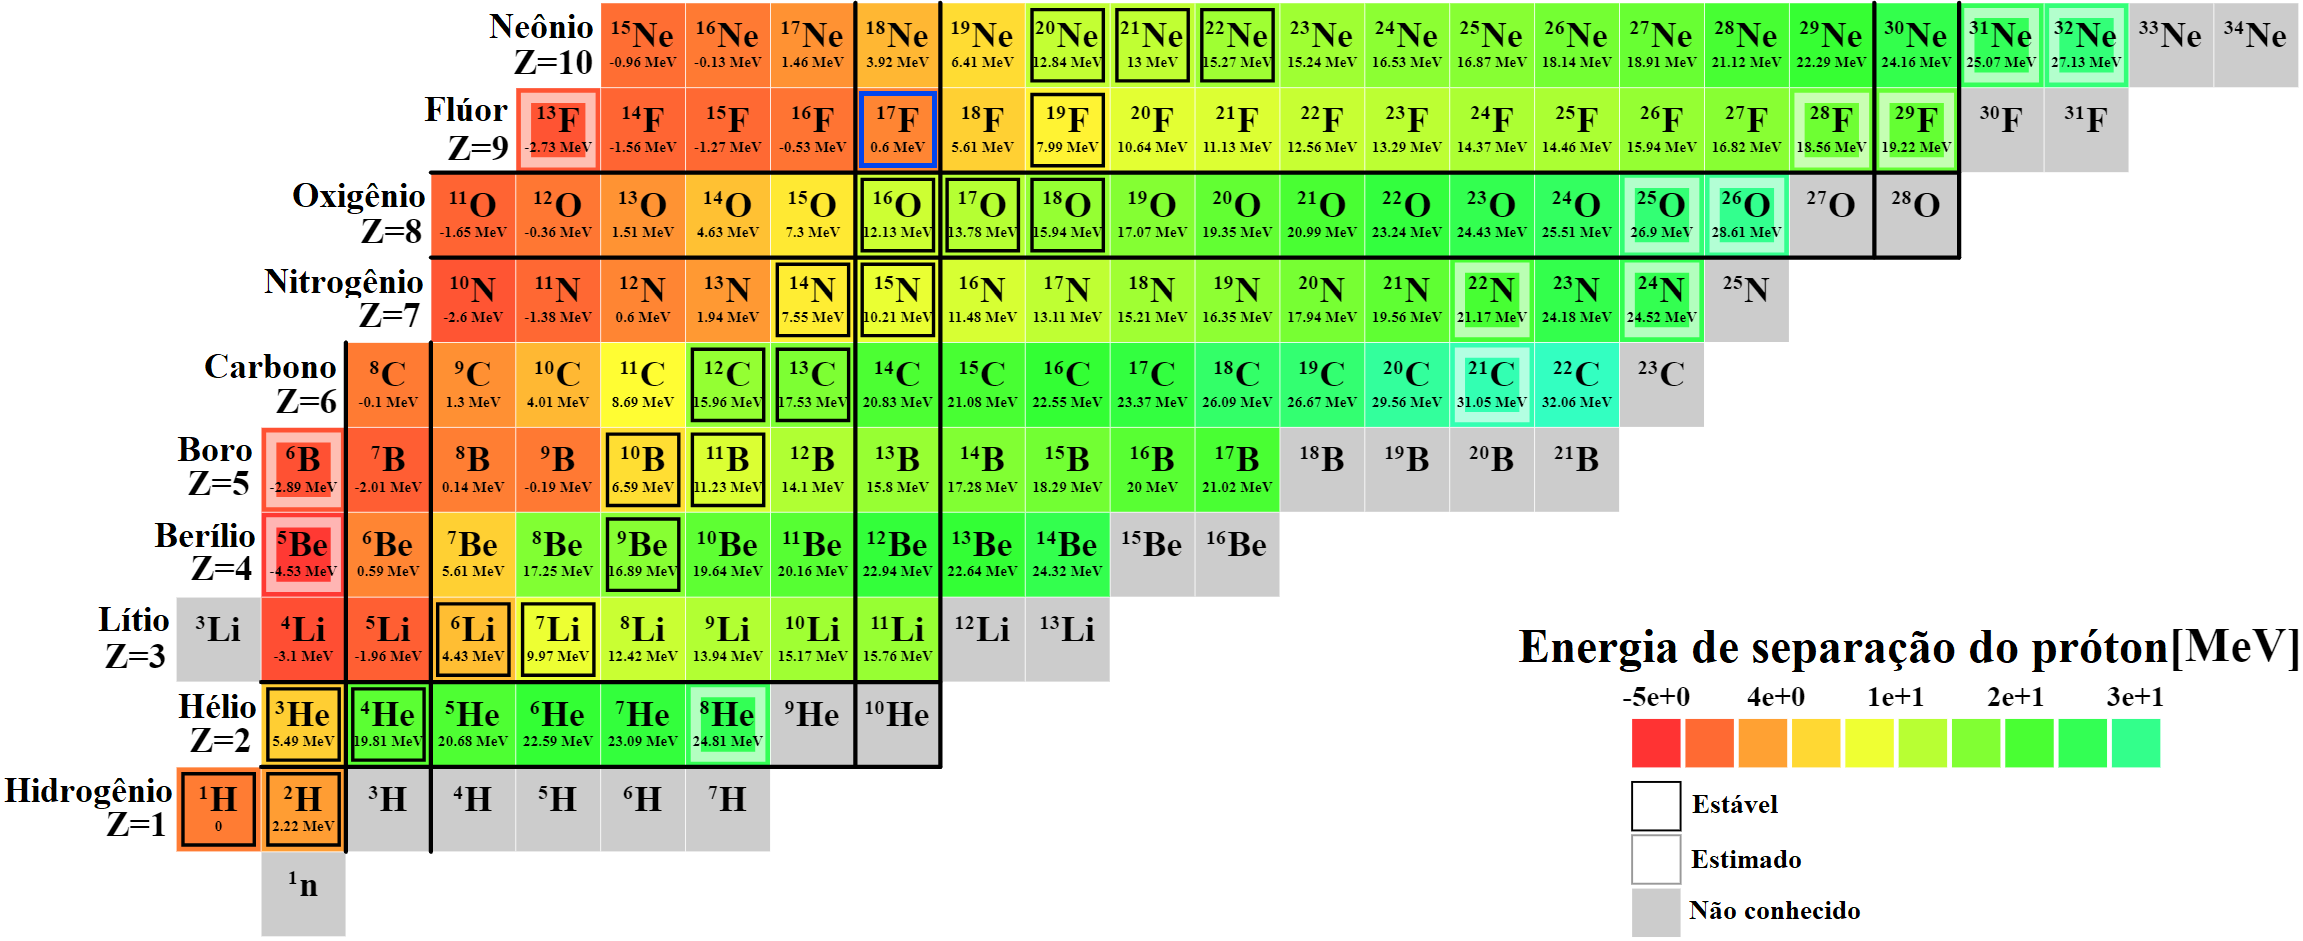
\includegraphics[scale = 0.25]{figs/chart_nuclides_2.png}
    \caption{Tabela de nuclídeos para elementos leves, indicando a energia de separação de um próton em MeV. O núcleo estudado nesse trabalho é o $^{17}$F (destacado pelo quadrado em cor azul), com $S_p$ = 600 keV. \cite{colourful_nuclide_chat}}
    \label{fig:chart_nuclides}
\end{figure}

\par Para investigar a estrutura de núcleos ricos em prótons ou em nêutrons, pode-se usar reações nucleares como o espalhamento elástico, transferência ou breakup \cite{Kolata2016}. Em particular, a reação de breakup é de grande importância para o estudo da estrutura dos núcleos radioativos ricos em prótons ou em nêutrons que possuem uma forte estrutura de cluster do tipo caroço + partículas de valência, onde as partículas de valência são fracamente ligadas \cite{Kolata2016, MORO_BREAKUP}. Quando a energia de ligação dessas partículas de valência é muito baixa, da ordem de centenas de keV até poucos MeVs, elas podem orbitar o caroço a grandes distâncias, formando uma configuração conhecida como ``estrutura halo". A reação estudada nessa dissertação é a reação de breakup $^4$He($^{17}$F,$^{16}$O+$p$)$^4$He, onde o $^{17}$F é um núcleo rico em prótons que forma uma estrutura halo formada por um núcleo que pode ser descrito como um núcleo de $^{16}$O mais um próton fracamente ligado ($S_p$ = 600 keV) \cite{MORO_BREAKUP}.

\par Para melhor caracterizar o mecanismo de uma reação de breakup, a identificação e detecção de ambos fragmentos da dissociação é muito importante. Para tanto equipamentos e sistemas de detecção complexos e sofisticados tem sido desenvolvidos. Um desses equipamentos é o Alvo Ativo. Conforme está explicado com detalhes ao longo dessa dissertação, o alvo ativo é um aparato que funciona tanto como alvo como sistema de detecção. O alvo ativo permite o uso de um gás específico que serve tanto quanto alvo quanto meio detector. Isso permite a detecção de múltiplas reações nucleares ao mesmo tempo, com a capacidade de medidas completas da cinemática das reações \cite{FORTINO2022166497, josh_bradt, attpc}. Com o alvo ativo é possível determinar as trajetórias tridimensionais das partículas envolvidas numa reação nuclear e reconstruir o respectivo vértice (posição da reação).


% Em medidas de breakup é importante identificar os fragmentos da dissociação dos núcleos fracamente ligados, necessitando um sistema de detecção sofisticado como o alvo ativo.



\par Nos últimos anos, alvos ativos envolvendo câmaras de projeção no tempo, \textit{active-target time projection chambers} (AT-TPCs), se tornaram importantes e relevantes para o estudo de núcleos exóticos em física nuclear \cite{FORTINO2022166497}. Diversos desses tipos de equipamentos foram desenvolvidos em diferentes laboratórios de física nuclear pelo mundo \cite{attpc, FURUNO2018215, KOSHCHIY2020163398}.

\par O sistema de detecção de TPCs, usualmente, é baseado na ideia de se detectar os elétrons provenientes da ionização do gás. Para tanto, foi desenvolvido um dispositivo que combina o micromegas (Micro-MEsh Gaseous Structures) \cite{micromegas} e o GEM (Gas Electron Multiplier) \cite{GET}. Esse dispositivo possui uma alta granularidade do plano detector, da ordem de 10$^3$ a 10$^4$ canais \cite{FORTINO2022166497}. Com isso, experimentos que envolvem TPCs produzem enormes quantidades de dados \cite{attpc, pattpc}. Por exemplo, o experimento analisado neste trabalho gerou cerca de 3 TB de dados crus em alguns dias de medida. Devido à grande quantidade de dados produzidos, a análise precisa ser dividida em diversas etapas, de modo que a eficiência e tempo computacional têm papel fundamental no processo. Nesse sentido, o uso de algoritmos como de machine learning pode trazer vantagens significativas para a análise. Esses algoritmos, por serem muito mais rápidos do que análise baseadas em algoritmos de programação convencional, podem viabilizar a análise dessa quantidade de dados num tempo razoável. Um dos objetivos desse trabalho foi exatamente o de desenvolver esse tipo de técnica para analise de dados obtidos de experimentos com alvos ativos. Alguns desses códigos e parte da análise desta dissertação já foram publicados em revistas indexadas internacionais \cite{FORTINO2022166497, artigo}.

%Diversos algoritmos foram desenvolvidos para a análise de diferentes etapas dos dados \cite{FORTINO2022166497, artigo}, porém o uso de algoritmos de machine learning pode trazer vantagens significativas para a análise. Um dos objetivos desse trabalho foi o de desenvolver este tipo de técnicas para a analise de experimentos com alvos ativos. Os algoritmos de machine learning viabilizam análises mais rápidas em comparação à algoritmos feitos em programação tradicional. Parte dos resultados desta dissertação já foram publicados em revistas internacionais \cite{artigo, FORTINO2022166497}.

% no Micro-MEsh GAseous Structures (micromegas) \cite{micromegas} e no Gas Electron Multiplier (GEM) \cite{GET}, que possui alta

\par A utilização de técnicas de machine learning já está sendo amplamente utilizada nas mais diversas área de nossa vida cotidiana (softwares de detecção de spam, sistemas de recomendação, marcação em fotos de redes sociais, assistentes pessoais ativados por voz, carros autônomos, smartphones com reconhecimento facial e muito mais). Essas técnicas estão agora sendo desenvolvidas e aplicadas para análise de dados obtidos de experiências científicas.

\par A dissertação está esquematizada da seguinte forma: no capítulo \ref{PATTPC} está feita a descrição do experimento cujos dados foram analisados; no capítulo \ref{sec:ml} está feita uma breve descrição do que é machine learning com exemplos de algoritmos e métodos utilizados; o capítulo \ref{chapter:sinais} foi dedicado para a análise dos sinais (pulsos) medidos no experimento; no capítulo \ref{chapter:point_cloud_analysis} está descrita a análise das nuvens de pontos reconstruídas a partir dos pulsos; no capítulo \ref{chapter:resultados} foi feita a construção das distribuições angulares bem como a análise e comparação com experimentos da literatura relacionados; por fim, no capítulo \ref{chapter:conclusao} está a conclusão do trabalho.

\chapter{O experimento}\label{PATTPC}

%\par Esse capítulo descreve sobre a parte experimental desse trabalho que foi desenvolvido na Universidade de Notre Dame em Outubro de 2019. O experimento foi feito usando o feixe radioativo $^{17}$F produzido pelo sistema TWINSOL (TWIN SOLenids) \cite{twinsol} e o alvo ativo pAT-TPC \textit{prototype Active Target - Time Projection Chamber} \cite{pattpc} foi usando como alvo e detector simultaneamente. Na continuação, está descrito como foi feito o sistema de produção do feixe secundário $^{17}$F e a detecção das reações induzidas por esse feixe no alvo ativo.

\par Esse trabalho corresponde a análise de dados obtidos da experiência onde foi medida a reação de breakup para o sistema ${}^{17}\mathrm{F}+{}^{4}\mathrm{He}$. Nessa experiência utilizamos um feixe de $^{17}$F, que é um núcleo radioativo com tempo de vida média de 64.37 segundos, incidindo sobre um alvo gasoso de $^{4}$He. A experiência foi realizada em outubro de 2019 na University of Notre Dame, Estados Unidos. O feixe radioativo de $^{17}$F foi obtido com o sistema de produção chamado TWINSOL \cite{twinsol} e conduzido até o alvo ativo pAT-TPC (prototype Active Target - Time Projection Chamber) \cite{pattpc}. Neste capítulo está descrito como o feixe radioativo ${}^{17}$F foi obtido e como os produtos da reação de breakup foram medidos.

% \par Primeiro será descrita a produção do feixe de $^{17}$F com foco na descrição do sistema de produção de feixes radioativos (TWINSOL). Na seção seguinte será apresentado o detector pAT-TPC.


% O objetivo deste experimento é fazer medidas do \textit{breakup} do  gasoso, com o prototype Active Target - Time Projection Chamber (pAT-TPC). Esse capítulo irá descrever a produção do feixe e a 

% \par O prototype Active Target - Time Projection Chamber (pAT-TPC) é um detector de alvo-ativo que usa o volume de gás tanto quanto alvo quanto como detector. Seu grande volume ativo e capacidade de rastreio (\textit{tracking}) fornecem boa resolução energética e  angular, o que torna o pAT-TPC adequado para trabalhar com feixes exóticos de baixa intensidade\cite{pattpc, pattpc2}. O feixe secundário de $^{17}$F usado pelo pAT-TPC é produzido pelo \textit{Twin Solenoids} (TWINSOL) \cite{twinsol}. A figura \ref{fig:twinsol+pattpc} mostra os dois sistemas acoplados.

% \par Essa seção irá descrever brevemente o pAT-TPC, bem como o TWINSOL. Descrições mais detalhadas podem ser encontradas nas referências \cite{pattpc, twinsol}.

% \section{Produção do feixe de $^{17}$F}
\section{Produção do feixe secundário $^{17}$F usando o sistema TWINSOL}\label{sec:twinsol}

\par O feixe radioativo $^{17}$F foi produzido em voo usando o sistema TWINSOL \cite{KOLATA1989503, NDtandem}. Um feixe primário de $^{16}$O foi acelerado a uma energia de 70 MeV e conduzido até a câmara de produção com uma intensidade da ordem de 200 nA. O alvo de de produção consiste de uma célula gasosa, preenchida com gás de deutério à uma pressão de 1 atm. A partir da reação de transferência de um próton ou um nêutron do feixe primário ($^{16}$O) com o alvo de produção (deutério), partículas como $^{17}$F e $^{17}$O foram produzidas \cite{KOLATA1989503, twinsol}. Essas partículas são selecionadas pelo sistema de duplo solenoides formando um feixe com essas partículas \cite{twinsol, ribras_leo}. A figura \ref{fig:twinsol+pattpc} mostra o desenho do sistema TWINSOL acoplado com o pAT-TPC.

%\par A produção do feixe radioativo $^{17}$F foi feita a partir da reação do feixe estável de $^{16}$O com um alvo de deutério gasoso. O feixe primário $^{16}$O foi produzido e acelerado por um acelerador tipo Tandem van de Graff do ISNAP (\textit{Institute for Structure and Nuclear Astrophysics}) localizado na Universidade de Notre Dame, Estados Unidos, que possui uma tensão terminal de até 10 MV \cite{KOLATA1989503, NDtandem}. O feixe de $^{16}$O foi conduzido até a câmara alvo de produção, preenchida com deutério, no início do sistema TWINSOL, onde partículas emergentes de reações nucleares surgiram ($^{17}$F, $^{16}$O, $^{17}$O). A figura \ref{fig:twinsol+pattpc} mostra o sistema TWINSOL acoplado com o pAT-TPC.

\begin{figure}[H]
    \centering
    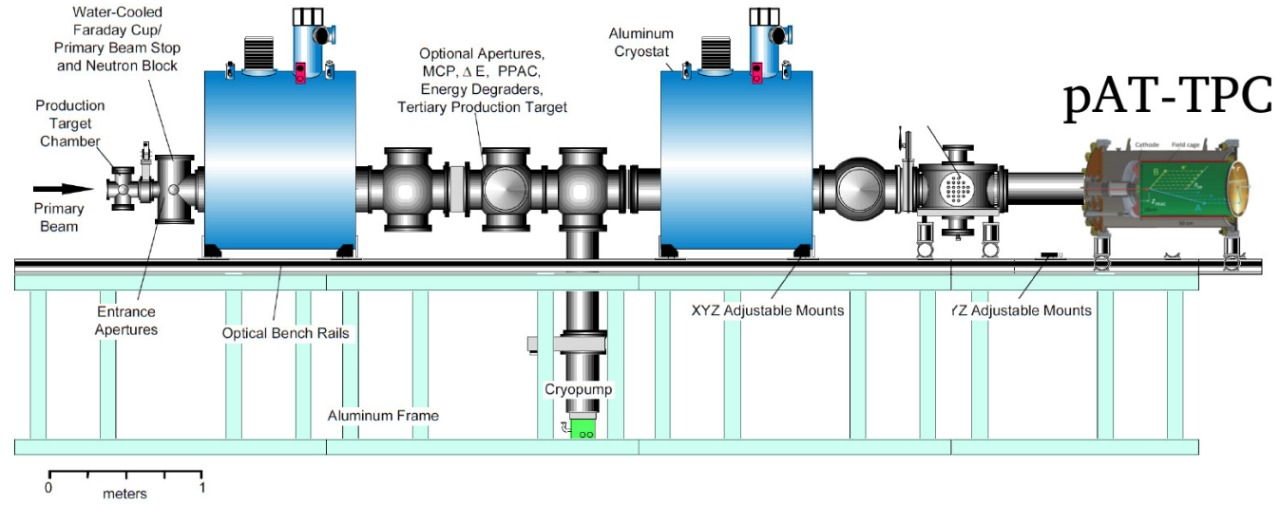
\includegraphics[scale = 0.35]{figs/poster3.jpeg}
    \caption{Desenho do TWINSOL à esquerda e do pAT-TPC à direita. O feixe estável de $^{16}$O entra à esquerda do TWINSOL, produzindo no alvo de produção o feixe secundário $^{17}$F que é conduzido até o alvo ativo pAT-TPC. Todo o sistema está localizado na University of Notre Dame.}
    \label{fig:twinsol+pattpc}
\end{figure}

\par O TWINSOL é um sistema de produção de feixes radioativos em voo que possui dois solenóides supercondutores alinhados que são usados para produzir, coletar, transportar, focar e selecionar feixes estáveis e radioativos. O sistema se baseia na seleção de partículas a partir da sua rigidez magnética ($B\rho$) \cite{twinsol, ribras_leo, zamora_mater}. Cada solenoide possui $15~\text{cm}$ de raio interno e 1 m de comprimento \cite{twinsol}. O fato de ser um solenoide finito faz com que surjam efeitos de borda na componente radial do campo magnético do solenoide, cujo efeito é fazer com que o solenoide seja capaz de selecionar e focalizar partículas \cite{ribras_leo}. Para entender melhor o efeito de borda no campo magnético, e consequentemente o funcionamento do TWINSOL, simulações computacionais usando a biblioteca GEANT4 \cite{geant4} foram feitas usando a geometria do sistema ``irmão" do TWINSOL, o \textit{Radioactive Ion Beams in Brasil} (RIBRAS), que também possui dois solenoides supercondutores alinhados \cite{ribras_leo, ribras}. A figura \ref{fig:sim_ribras} mostra a geometria usada na simulação, onde os solenoides são de cor verde focalizando as partículas de cor laranja em um ponto do plano focal em vermelho. O campo magnético usado na simulação é função da posição do eixo, de cada solenoide, e está mostrado na figura \ref{fig:campo_mag}.


% A figura  mostra um exemplo de calculo do valor do campo magnético, usando valores do sistema , para as componentes $x$, $y$ e $z$. É nítido que o campo em $z$ permanece praticamente constante e próximo das extremidades da bobina (linha vertical tracejada preta), $B_x$ e $B_y$ crescem em módulo, fazendo com que o solenoide funcione como uma lente delgada.

\begin{figure}[H]
    \centering
    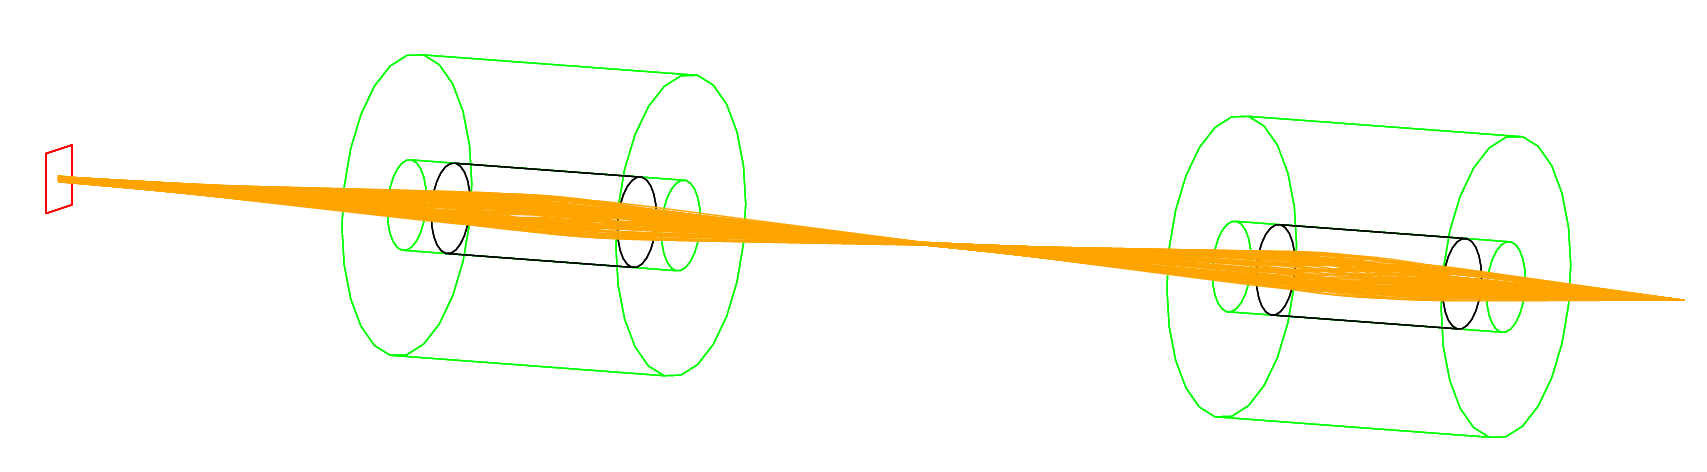
\includegraphics[scale = 0.95]{figs/Foco2S.png}
    \caption{Simulação computacional do sistema RIBRAS, onde as partículas carregas em laranja surgem do ponto à direita da figura e passam pelos dois solenoides em verde, para então serem focalizadas em um ponto do plano focal em vermelho. A parte em preto dos solenoides corresponde aos limites físicos da bobina \cite{ribras_leo}.}
    \label{fig:sim_ribras}
\end{figure}

\begin{figure}[H]
    \centering
    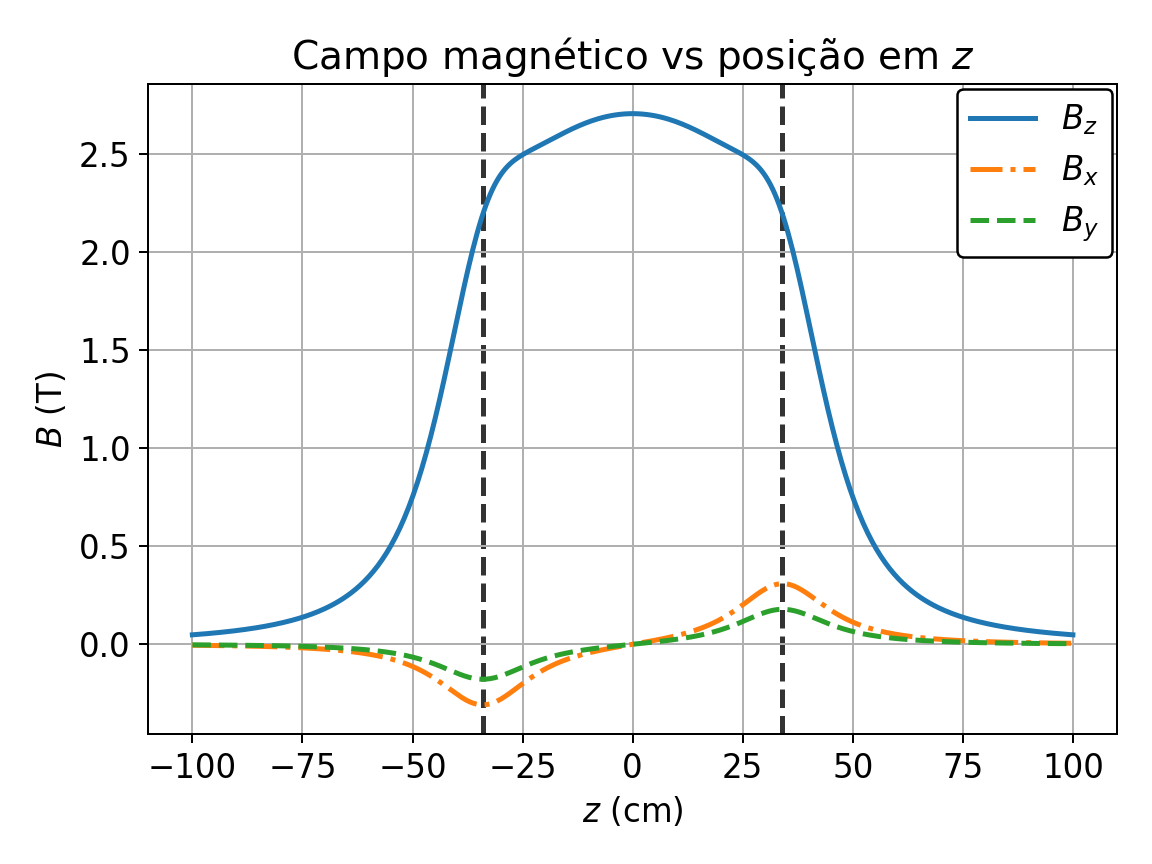
\includegraphics[scale = 0.85]{figs/Campo_mag.png}
    \caption{Valor do campo magnético $B$ em tesla em função da posição em $z$ em centímetro da bobina. A linha vertical tracejada preta indica o limite físico da bobina. O campo foi calculado à uma distância de 8 cm do eixo do solenoide. É possível ver claramente o efeito de borda que há em um solenoide finito \cite{magnetic_field}.}
    \label{fig:campo_mag}
\end{figure}


\par Apesar de não ser evidente na figura \ref{fig:sim_ribras}, a trajetória as partículas dentro do solenoide são helicoidais devido à força de Lorentz e possuem uma determinada frequência de ciclotron \cite{ribras_leo}. Além disso, cada solenoide se comporta como uma lente grossa usada para focalizar os feixes. Em uma aproximação de um solenoide como uma lente grossa, o foco depende da rigidez magnética da partícula através da relação \cite{KOLATA1989503, zamora_mater}:

\begin{equation}
    \frac{1}{f} = \frac{B_z ^2}{(B\rho)^2},
\end{equation}
%
onde $f$ é o ponto focal, $B_z$ a componente $z$ do campo magnético, e $B\rho$ é dado por:
%
\begin{equation}
    B\rho = \frac{mv}{q} = \frac{\sqrt{2mE}}{q},
\end{equation}
%
onde $E$ é a energia, $m$ sua massa e $q$ seu estado de carga.

%\par Para produzir $^{17}$F, uma célula gasosa localizada na câmara alvo de produção\cite{twinsol} preenchida com deutério foi bombardeada pelo feixe primário. Além de $^{17}$F, outras partículas também foram geradas, como o $^{17}$O, além de $^{16}$O do feixe espalhado.

\par No experimento, os campos magnéticos dos solenoides foram ajustados para focalizar o feixe de $^{17}$F dentro do pAT-TPC, com energia de 51 MeV e intensidade da ordem de 10$^2$ $\sim$ 10$^3$ partículas por segundo. No entanto, partículas com energias e massas diferentes mas com o mesmo $B\rho$ (ou valores próximos) do feixe de interesse poderiam ser também selecionadas pelos solenoides. Isso faz com que não seja possível obter um feixe de $^{17}$F com 100\% de pureza, e sim um coquetel de partículas \cite{zamora_mater}. O coquetel de feixe produzido nesse experimento tinha 54\% de $^{17}$F, 41\% de $^{16}$O e cerca de 5\% de $^{17}$O. A figura \ref{fig:PID_17F} mostra o espectro biparamétrico de identificação de partículas obtido durante o experimento, onde é possível identificar as partículas que estão presentes no feixe (coquetel de partículas). Por fim, o feixe produzido pelo TWINSOL foi conduzido até o pAT-TPC.

\begin{figure}[H]
    \centering
    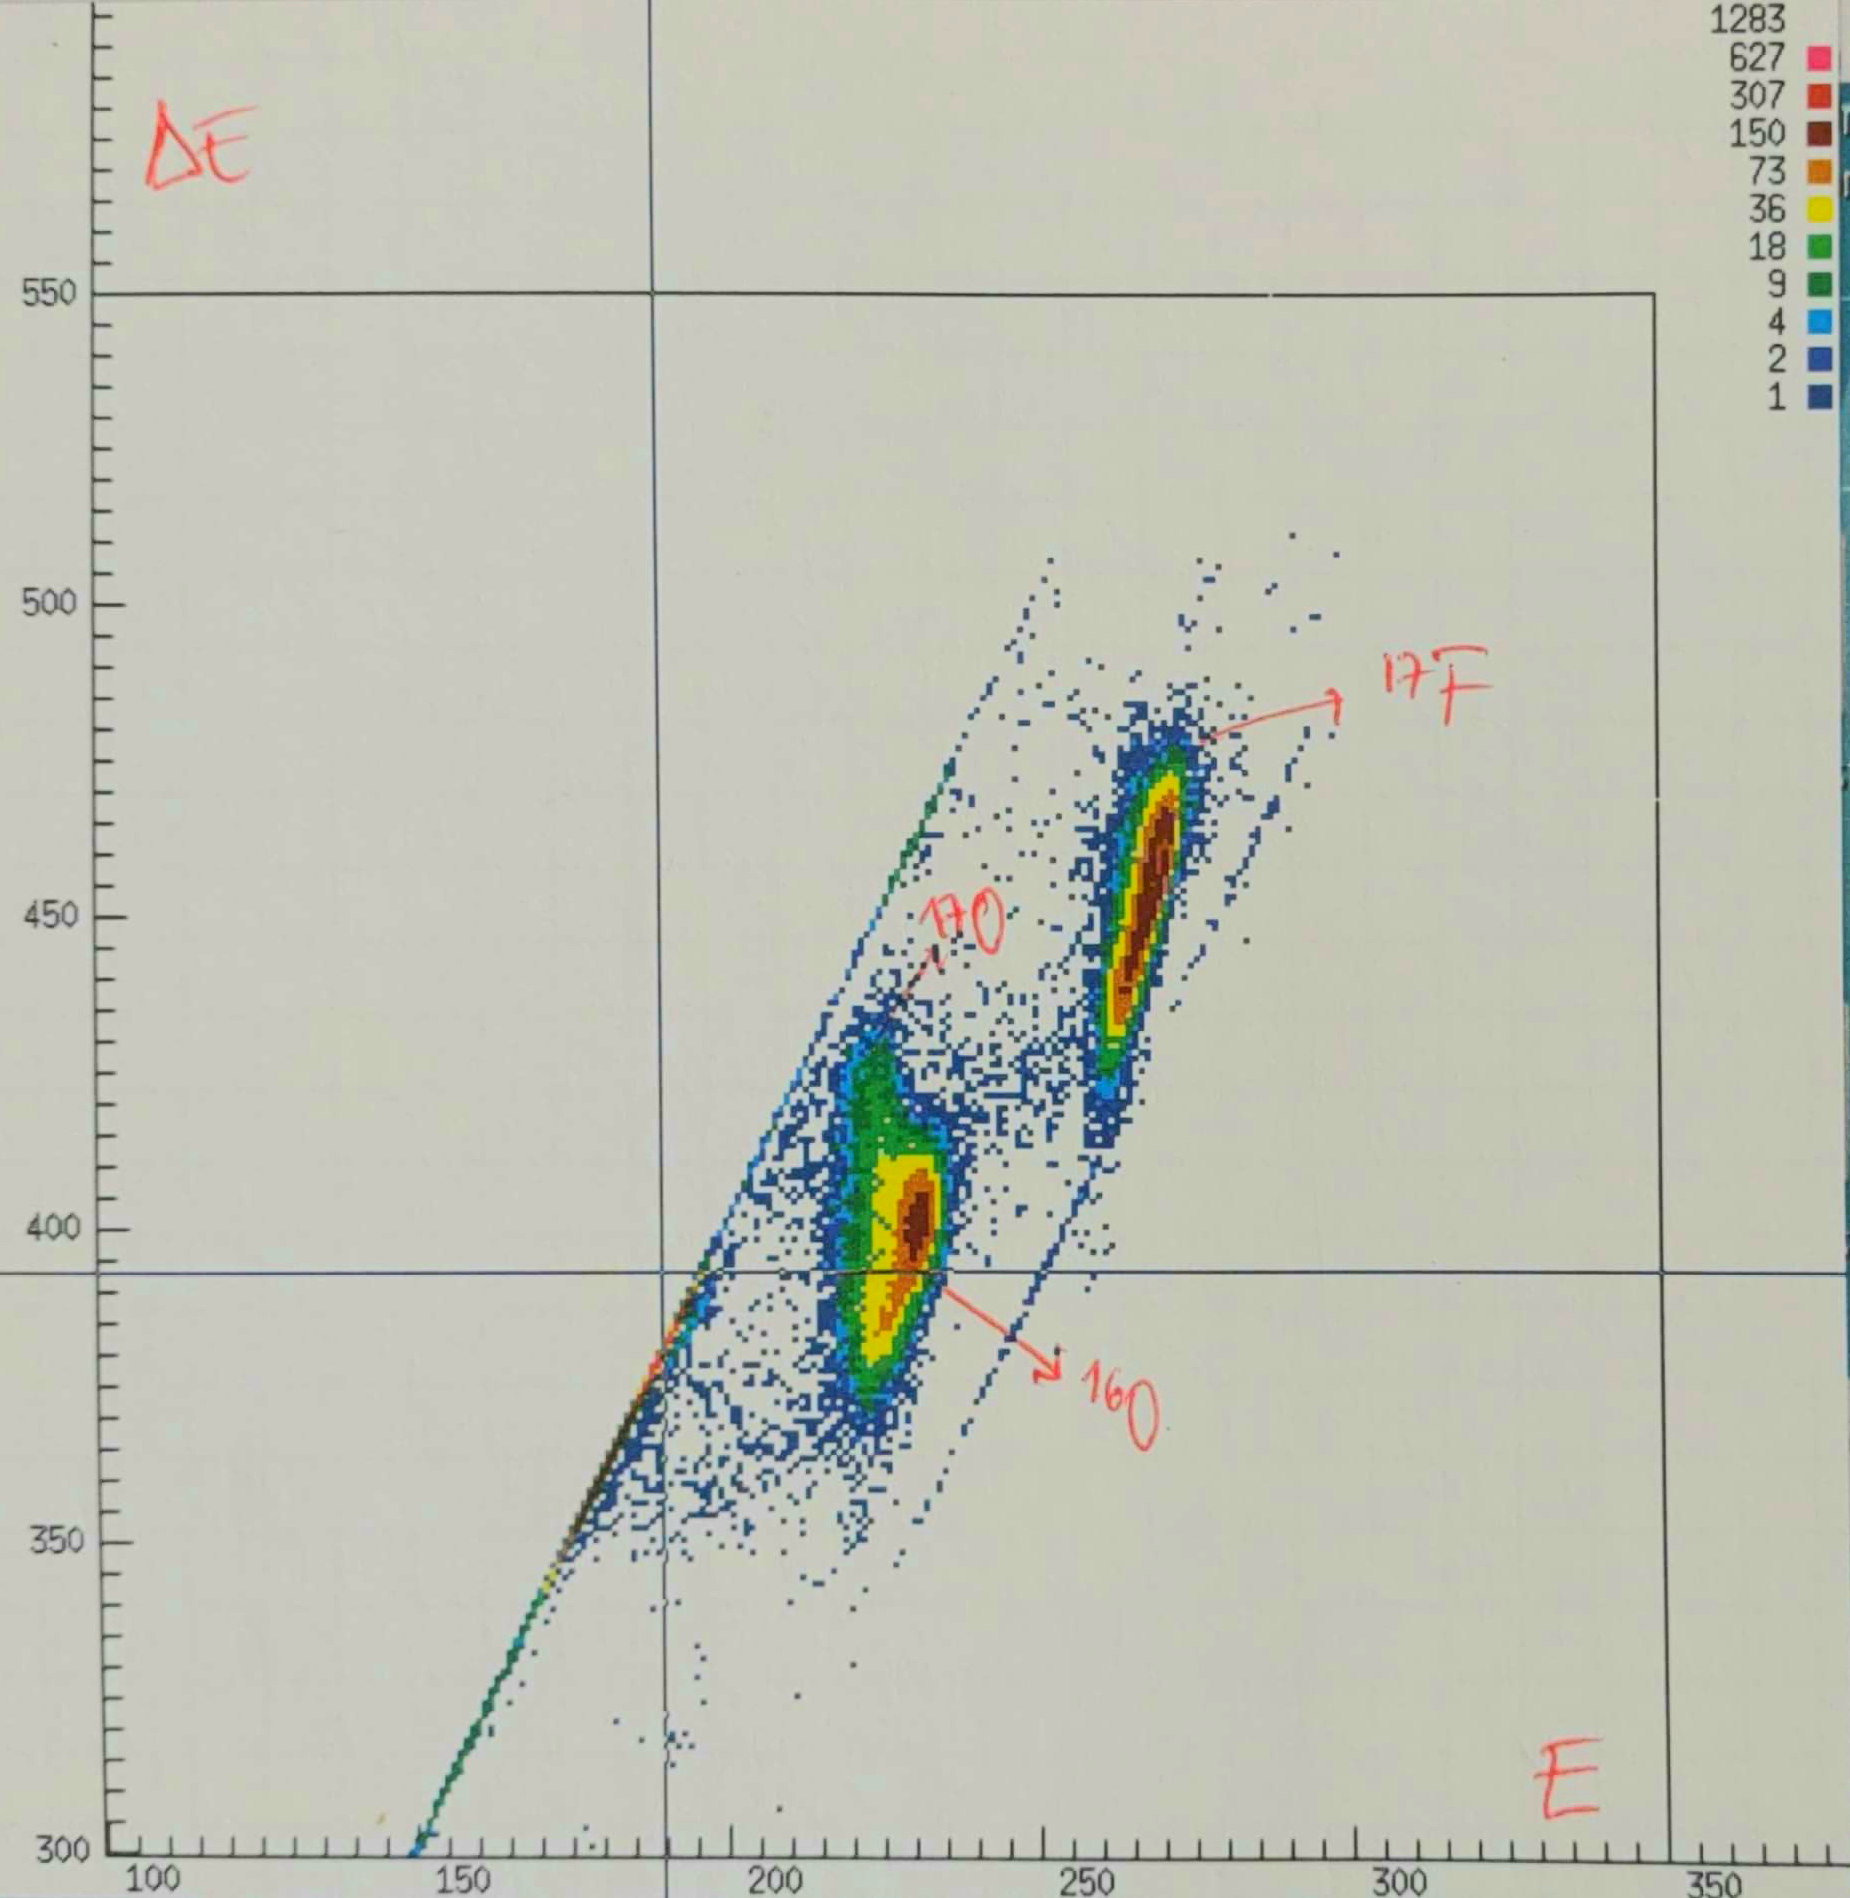
\includegraphics[scale = 0.12]{figs/pid_17F.png}
    \caption{Espectro biparamétrico $\Delta E$ - $E$ de identificação de partículas. Nele é possível identificar que o feixe possui a presença de $^{17}$F, $^{16}$O e uma pequena parte de $^{17}$O.}
    \label{fig:PID_17F}
\end{figure}

\par Para identificar essas partículas do coquetel de feixe um sistema de detectores, formando um telescópio $\Delta E$--$E$, foi posicionado à 50 cm da janela do pAT-TPC, em zero graus com relação ao eixo $z$ da câmara. Uma vez preparado o feixe, ele foi removido. O espectro biparametrico formado pela combinação dos sinais $\Delta E$ versus $E_{\mathrm{total}}$= $\Delta E$ + $E_{\mathrm{residual}}$, permite a identificação das partículas. 

\section{O alvo ativo pAT-TPC}

%\par Essa seção irá descrever brevemente propriedades geométricas e físicas relacionadas ao sistema de detecção usado neste experimento, o alvo ativo pAT-TPC.
%  O pAT-TPC é um detector preenchido com gás que é usado como alvo-ativo.

\par O sistema de detecção utilizado nessa experiência foi o alvo ativo pAT-TPC. Alvos ativos vêm sendo cada vez mais utilizados em experimentos para investigações de reações nucleares \cite{FORTINO2022166497}, dentre os diversos laboratórios que utilizam alvos ativos podemos citar o TexAT \cite{KOSHCHIY2020163398} e o ACTAR \cite{MAUSS2019498}. A principal razão é que esses alvos funcionam também como detectores permitindo uma total identificação das partículas e de suas trajetórias dentro do alvo.

\par A figura \ref{subfig:pattpc} mostra o desenho esquemático do pAT-TPC, que foi o alvo ativo utilizado no experimento. O detector possui uma cela cilíndrica de 50 cm de comprimento e 28 cm de diâmetro, onde o seu eixo (direção $z$) é alinhado com o eixo do feixe \cite{pattpc}, que passa pela câmara de íons no duto central. Para que o gás (utilizado como alvo) seja confinado dentro dessa câmara, utilizamos janelas finas o bastante para permitir a passagem do feixe, mas grossas o suficiente para o confinamento do gás. O feixe de $^{17}$F, com energia inicial de 51 MeV, entra na câmara passando pela janela. O feixe radioativo de $^{17}$F, com energia inicial de 51 MeV, perde energia durante a passagem pela janela (feita de PPTA - \textit{p-phenylene terephthalamide} - com 12 $\mu$m de espessura) do pAT-TPC ficando com 34.76 MeV. Nesse experimento, a câmara foi preenchida com $^4$He gasoso puro à uma pressão de 350 Torr que serve tanto como alvo para as reações nucleares, quanto para a própria medição e detecção dos produtos da reação \cite{pattpc, pattpc2}. Tanto o feixe quanto as partículas originadas pelas reações que possam ocorrer ionizam o gás e os elétrons que surgem dessa ionização são conduzidos por um campo elétrico de 1 kV/cm perpendicular ao eixo da câmara até o plano detector (\textit{pad plane}), o micromegas \cite{micromegas}, localizado no final da câmara, mostrado na figura \ref{subfig:micromegas}.


%Durante a passagem pela câmara de íons e pela janela (feita de PPTA - p-phenylene terephthalamide - com 12 $\mu m$ de espessura) do pATTPC, o feixe $^{17}$F perde energia e entra na câmara com cerca de 34.76 MeV. 



\begin{figure}[H]
\centering
    \begin{subfigure}[t]{0.49\textwidth}
        \centering
        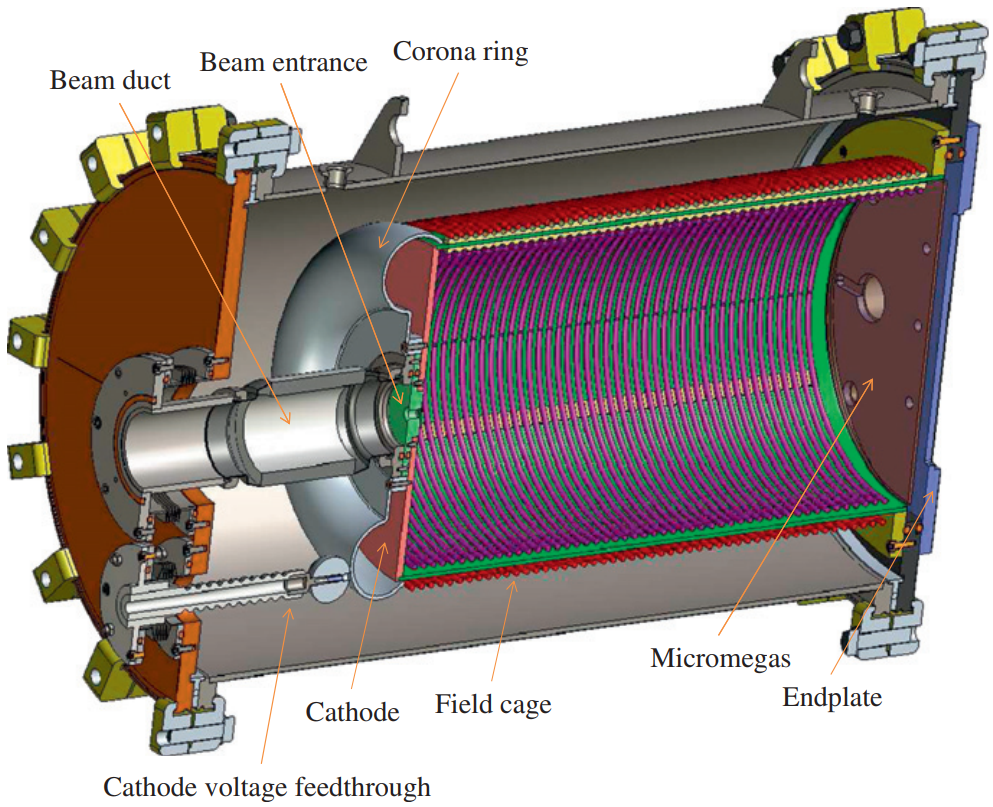
\includegraphics[scale=0.30]{figs/pattpc.png}
        \caption{Visão transversal do pAT-TPC. O gás é preenchido dentro da cela que possui um campo elétrico perpendicular ao plano do micromegas, à direita da figura. O feixe incide na câmara entrando pelo duto de feixe à esquerda da figura.}
        \label{subfig:pattpc}
    \end{subfigure}%
    \hfill
    \begin{subfigure}[t]{0.49\textwidth}
        \centering
        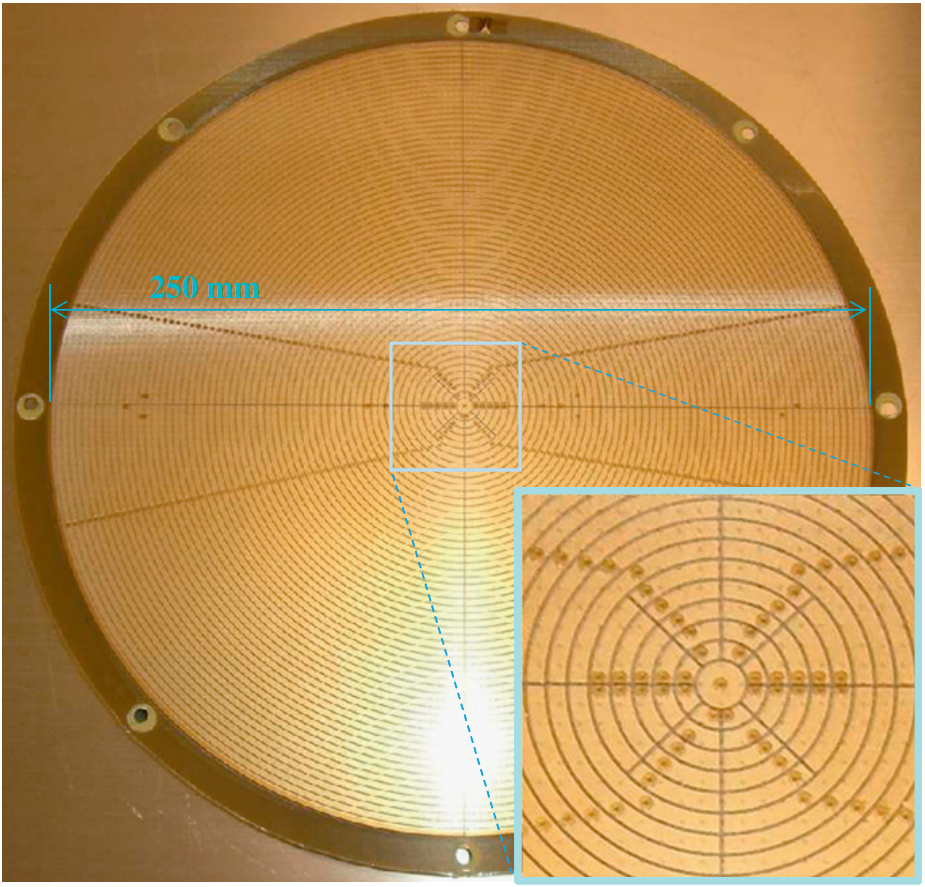
\includegraphics[scale=0.28]{figs/micromegas.png}
        \caption{Foto do micromegas. O detector é multipixelado com uma maior densidade no centro, parte destacada na imagem. O \textit{pad} central tem diâmetro de 5 mm enquanto que as faixas coaxiais possuem passo de 2 mm \cite{attpc, josh_bradt}.}
        \label{subfig:micromegas} 
    \end{subfigure}
\caption{Figura esquemática do pAT-TPC e o detector micromegas\cite{pattpc}.}
\label{fig:pattpc_e_micromegas}
\end{figure}

\par O micromegas é um dispositivo de amplificação de elétrons, que consiste em um plano detector com 2048 canais (pads) triangulares (ver o design do plano detector na figura \ref{fig:padplane} com eletrônica independente, que usa o \textit{Generic Electronics for TPCs} (GET) \cite{GET}. Detalhes sobre a eletrônica podem ser encontrados nas Refs. \cite{GET, josh_bradt}. Cada pad do micromegas possui uma posição ($x$, $y$) fixa e a terceira coordenada $z$ é determinada a partir do tempo de deriva dos elétrons no gás \cite{pattpc, pattpc2, attpc, josh_bradt}. Isso só é possível pois a velocidade de deriva (\textit{drift}) dos elétrons é constante \cite{drift_constant}, portanto a posição em $z$ da partícula é diretamente proporcional ao tempo de deriva. Esse princípio que deu origem ao nome de \textit{Time Projection Chamber}, pois o evento é projetado no tempo de deriva dos elétrons no gás.

\begin{figure}[H]
    \centering
    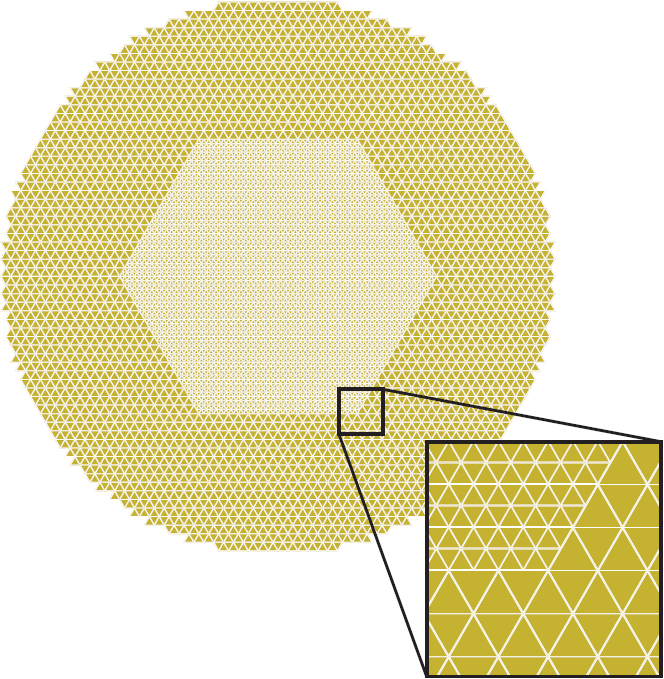
\includegraphics[width=0.65\textwidth]{figs/padplane.png}
    \caption{Design do plano detector. A densidade de pads é maior na região central. Com o zoom em um dos vértices da parte hexagonal é possível ver o formato triangular dos pads.}
    \label{fig:padplane}
\end{figure}

\par A coordenada $z$ depende da velocidade de deriva (\textit{drift velocity}) dos elétrons no gás. A equação \ref{eq:langevin} (equação de Langevin) descreve o movimento de um elétron com massa $m$ e carga $e$ sujeito a um campo elétrico e magnético \cite{drift_constant}

\begin{equation}\label{eq:langevin}
    m\frac{d\vec{v}}{dt} = e\left(\vec{E} +\vec{v}\times \vec{B}\right) - \frac{m}{\tau}\vec{v},
\end{equation}
%
onde $\vec{E}$ é o vetor campo elétrico, $\vec{B}$ o vetor campo magnético, $\vec{v}$ é o vetor de velocidade do elétron e $\tau$ é o tempo de colisão médio, que depende das propriedades termodinâmicas do gás. No caso deste experimento, $\vec{B}$ é zero e a solução estacionária para a velocidade de deriva do elétron é

\begin{equation}\label{eq:v_tpc}
    \vec{v} = \frac{\tau}{m}e\vec{E}.
\end{equation}

\par A velocidade de deriva depende das propriedades termodinâmicas do gás (temperatura, pressão) e também de sua condutividade elétrica \cite{drift_constant}. Isso significa que a calibração da velocidade não depende só do campo elétrico, mas também das propriedades do gás dentro do alvo ativo \cite{pattpc, drift_constant}. Para acharmos a coordenada $z$, basta integrar a equação \ref{eq:v_tpc} para obter

\begin{equation}
    z = \frac{\tau}{m}e\vec{E}(t - t_0),
\end{equation}
%
onde no tempo $t_0$ = 0 o elétron está no plano do detector ($z$ = 0).

\par A velocidade de deriva do elétron no gás de $^4$He puro deveria ser sempre constante, se as condições permanecessem as mesmas durante toda o experimento. No entanto, nas medidas desse experimento, essa velocidade variou um pouco a cada run (conjunto de eventos para serem analisados). A figura \ref{fig:vdrif_vs_run} mostra a velocidade de deriva obtida para cada run ($\sim$ 1 h) do experimento.

\begin{figure}[H]
    \centering
    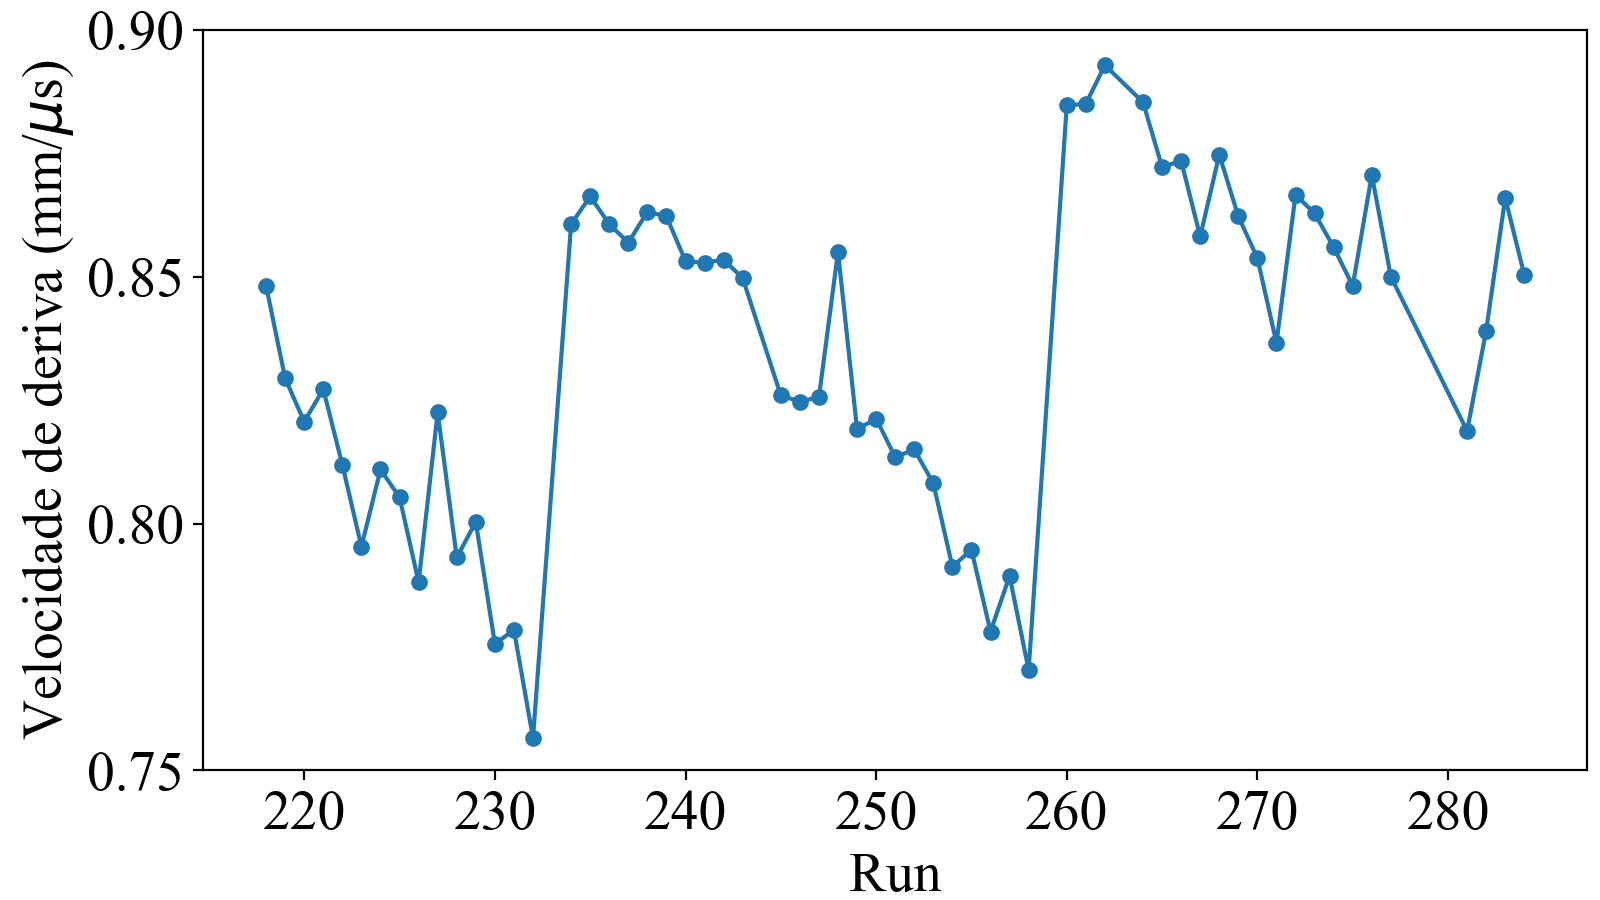
\includegraphics[width=0.85\textwidth]{figs/vdrift_vs_run.png}
    \caption{Gráfico de velocidade de deriva dos elétrons a cada run. O tempo de duração de cada run foi de aproximadamente uma hora.}
    \label{fig:vdrif_vs_run}
\end{figure}

\par Pela figura \ref{fig:vdrif_vs_run} é perceptível que a velocidade de deriva dos elétrons no gás teve uma variação por volta do 10\% durante o experimento. A queda na velocidade ocorre, por exemplo, por problemas relacionados à impurezas no gás devido à filtragens de ar dentro do gás (ou \textit{outgassing}) de alguns materiais dentro do alvo. Foi necessário corrigir os dados experimentais run por run a partir desses valores de velocidade de deriva.

\par Por exemplo, para o run 218, a velocidade de deriva dos elétrons foi aproximadamente de 0.85 cm/$\mu$s. Isso significa que os elétrons produzidos próximo na janela de entrada do detector percorrem os 50 cm da câmara em cerca de 59 $\mu$s. Dividindo esse tempo pelos 512 canais (largura de cada bin dos pulsos gerados), tem-se que cada canal (time bucket) possui cerca de 115 ns de largura.

\par O pAT-TPC conta com uma camada extra de \textit{thick gems} acoplada ao detector micromegas. \textit{Thick gems} usam do fato de que, no momento em que o elétron passa para uma região de campo elétrico ordens de grandeza maior que de sua origem, ocorre a ionização secundária (quando o elétron ioniza o gás). Isso provoca o que é chamado de avalanche de elétrons, amplificando a intensidade do sinal recebido \cite{GET}. A camada com \textit{thick gems} fica por volta de 100 $\sim$ 120 $\mu$m do pad plane, com um campo elétrico 10 vezes maior que o campo elétrico da câmara. A figura \ref{fig:thick_gems} mostra a esquematização do micromegas, onde na eletrônica de saída é produzido um sinal em função do tempo.

\begin{figure}[H]
    \centering
    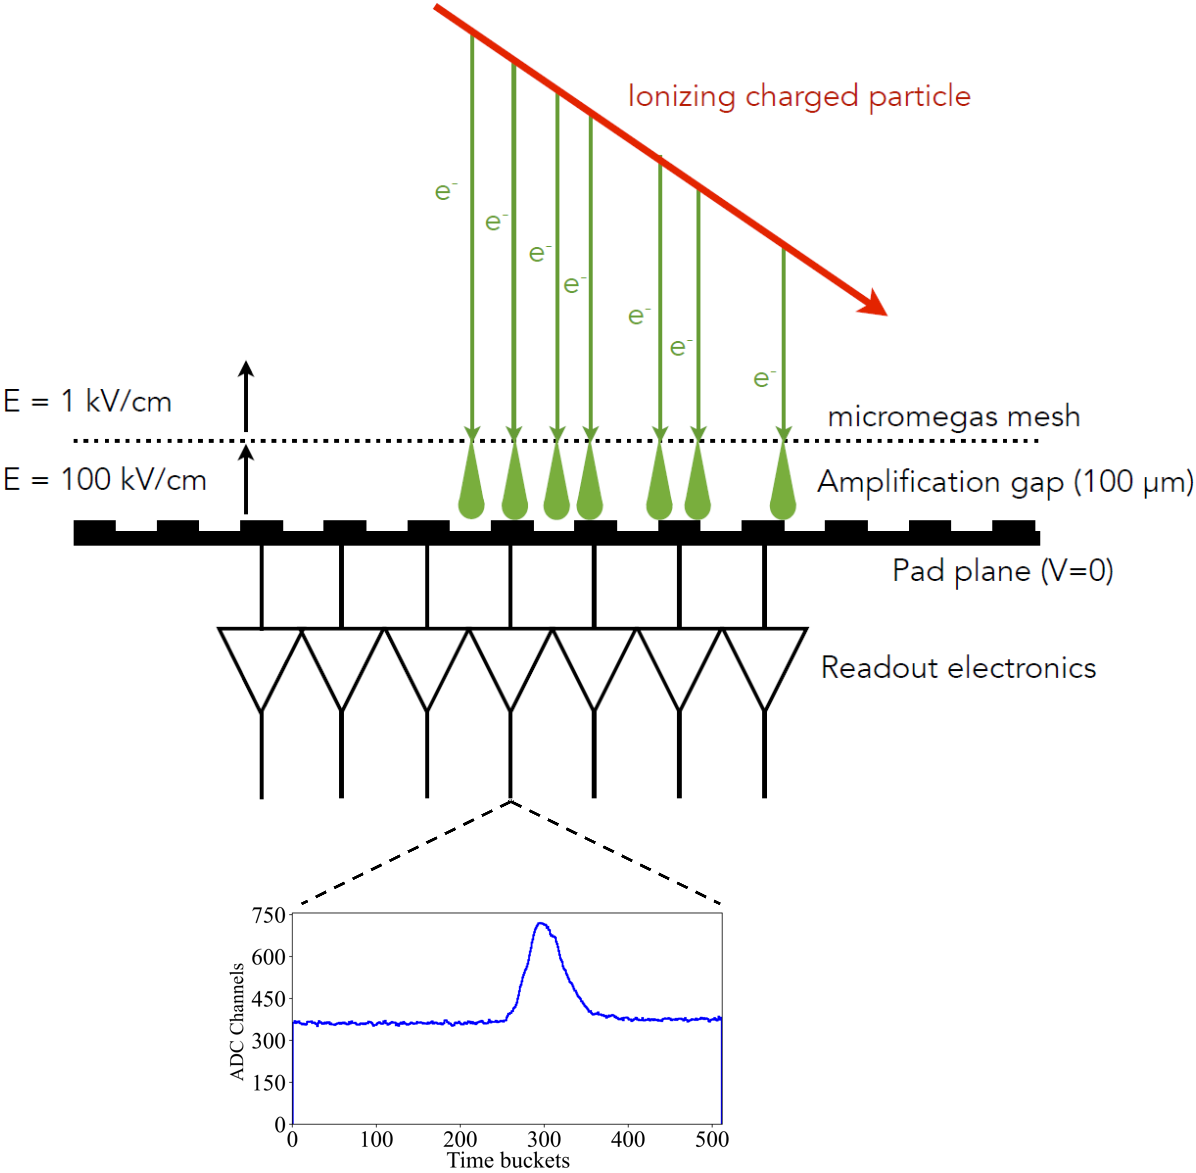
\includegraphics[scale = 0.40]{figs/thick_gems_2.png}
    \caption{Plano do micromegas com a esquematização das \textit{thick gems}. Os elétrons quando passam para um campo elétrico mais intenso ionizam o gás, produzindo ainda mais elétrons (evento chamado de avalanche de elétrons). Cada canal da eletrônica de saída produz um pulso como mostrado na parte de baixo da figura.}
    \label{fig:thick_gems}
\end{figure}

%\par O sinal é discretizado no tempo levando em conta a velocidade de deriva dos elétrons, dividindo em 512 canais o tempo que o elétron leva para percorrer toda câmara do TPC \cite{josh_bradt, pattpc}.

\par Cada interação de uma partícula carregada com o gás (liberação de elétrons por ionização do gás) é detectada como um pulso eletrônico, onde o centróide corresponde ao tempo de deriva. A carga acumulada $Q$ dessa interação é a área do pulso associado ao centroide. Cada centroide então representa um ponto no espaço ($x$, $y$, $t$, $Q$). Um exemplo de evento reconstruído está na figura \ref{fig:event_cap_exp}.

\begin{figure}[H]
    \centering
    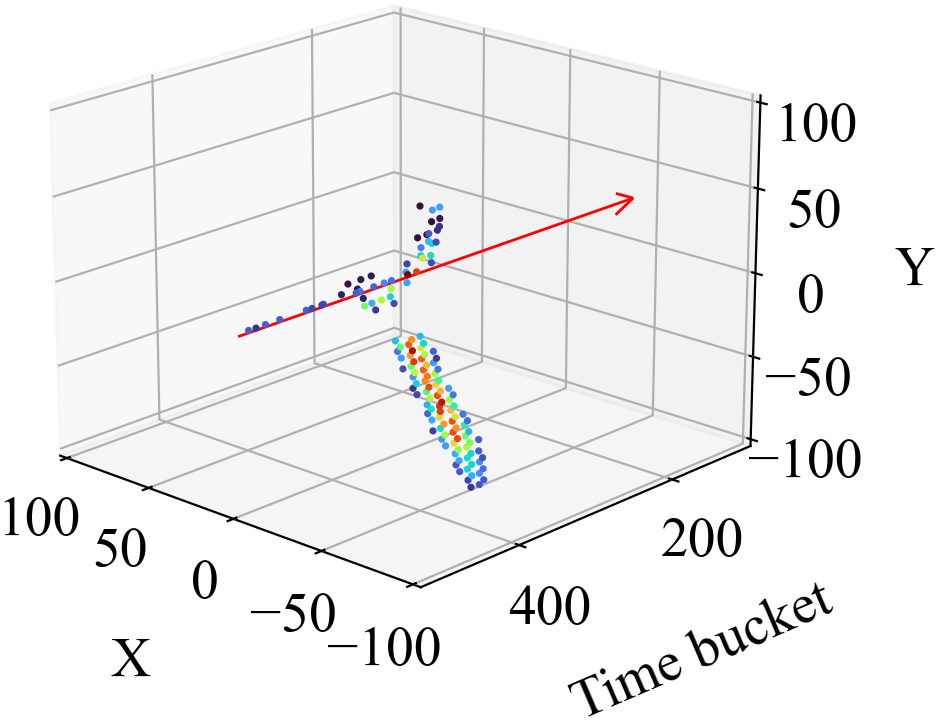
\includegraphics[scale = 0.40]{figs/event_cap_exp.png}
    \caption{Evento reconstruído a partir da análise dos pulsos gerados pelo micromegas. A cor representa a carga integrada de cada ponto de interação com o gás.}
    \label{fig:event_cap_exp}
\end{figure}
% Existem canais auxiliares que servem para evitar armazenar canais sem detecção. Caso haja detecção além do centro do micromegas então os sinais gerados pelo evento são armazenados \cite{josh_bradt, attpc}.

\par Cada evento produz em média 300 pulsos. Para que fosse possível reconstruir as trajetórias das partículas, foi preciso analisar cada um desses 300 pulsos de todos os eventos da trajetória. No entanto, o número de evento reconstruídos é da ordem de milhões, portanto a quantidade de sinais que precisam ser analisados é de grandes proporções, em comparação com experimentos no passado em física nuclear onde apenas alguns canais de detecção são utilizados, gerando um evento por canal. É essa grande quantidade de dados também gerou a necessidade de desenvolvimento de algoritmos com alta eficiência em tempo para que a análise seja muito mais rápida. Justamente esse é um dos principais objetivos desse trabalho, que é desenvolver algoritmos de machine learning para a análise de dados com o alvo ativo. Para a análise completa do nosso experimento foram seguidas as seguintes etapas:

% \par Nem todos os \textit{pads} do detector são ativados por evento. Existem canais auxiliares que servem para evitar armazenar canais sem detecção. Caso haja detecção além do centro do micromegas então os sinais gerados pelo evento são armazenados\cite{josh_bradt, attpc}. São gerados cerca de 300 sinais por evento, sendo que existem milhões de eventos, o que gera a necessidade de desenvolvimento de algoritmos extremamente eficientes em tempo para a análise. Para a análise completa do experimento precisamos seguir as seguintes etapas:

\begin{itemize}
    \item Análise dos pulsos de cada interação das partículas com o gás. Isso envolve remover o fundo, localizar os picos e obter os tempos e carga integrada de cada caso;
    \item Reconstruir eventos (trajetória das partículas) em 3D (nuvens de pontos) a partir da análise de sinais. As nuvens de pontos precisam ser analisadas com algoritmos de reconhecimento de padrões que permitem ajustar as trajetórias das partículas em 3D;
    \item Reconstruir a cinemática das partículas com as trajetórias e energia depositada no gás. Isto permite obter as distribuições angulares. 
\end{itemize}

% \begin{itemize}
%     \item Reconstruir os eventos tridimensionais (nuvens de pontos) a partir dos sinais gerados pelo micromegas. Isso inclui remover o fundo, localizar todos os pontos de interação das partículas carregadas com o gás etc. Isso será mostrado em detalhes no capítulo \ref{chapter:sinais};
%     \item A partir das nuvens de pontos é necessário reconstruir a cinemática das reações, identificando trajetórias das partículas e o vértice de reação;
%     \item Com a cinemática reconstruída podemos associar as partículas com as trajetórias e finalmente construir as seções de choque. 
% \end{itemize}

\par A descrição completa da análise dos pulsos, reconstituição de eventos, reconstrução da cinemática, gráficos das distribuições angulares e resultados são apresentadas nos próximos capítulos.

% \chapter{Uma breve introdução ao \textit{Machine Learning}}\label{sec:ml}
\chapter{Desenvolvimento de ferramentas de \textit{machine learning} para analise de dados}\label{sec:ml}

\par Uma das possibilidade para que possamos analisar a grande quantidade de dados gerados em experimentos com alvo ativo é a utilização de técnicas de machine learning. Nesse capítulo explicamos a metodologia usada para a implementação dessas ferramentas para a análise dos dados obtidos na experiência realizada com ${}^{17}\text{F}+{}^{4}\text{He}$. O apêndice \ref{appendix:ml_nuclear} mostra algumas aplicações recentes de machine learning na física nuclear.

\par De modo geral, machine learning é a utilização de algoritmos para extrair informações de uma grande quantidade de dados brutos e representá-los através de algum tipo de modelo matemático. Machine learning é, portanto, uma técnica onde os algoritmos analisam os dados aprendendo (ou sendo ensinado) com eles, sem que tivessem sido explicitamente programados para isso \cite{mlbook}. A ideia de machine learning não é nova e surgiu na década de 50 \cite{curso, mlbook}. No entanto, somente nos dias de hoje, com a possibilidade de processamento paralelos de CPU é que ela pode ser aplicada. Essa ideia de processamento foi também inspirada no funcionamento da rede neural biológica, onde os neurônios interagem enviando sinais através de conexões que se desenvolvem com treinamento. Aqui as interações seriam os sinais na forma de funções matemáticas enviadas ou trocadas entre as camadas, que poderiam ser associados aos neurônios. Aqui então, uma rede neural seria uma sucessão de camadas interligadas por operações e funções matemáticas. Isso inspirou o uso do modelo matemático simples de uma função linear nos parâmetros para um neurônio artificial ou camada \cite{curso}:

\begin{equation}\label{eq:model_n}
    y = f\left(\sum^{n}_{i = 1}\omega_i x_i + b_i\right) = f(z),
\end{equation}
%
%onde $y$ é a saída do neurônio, que corresponde à função de ativação $f$ que depende da soma ponderada, onde o peso é $\omega_i$, das entradas $x_i$ dos outros $n$ neurônios.
onde $y$ é o resultado da função matemática da interação entre os neurônios (camadas), dada pela função de ativação $f$. Essa função $f$ é dada pela soma ponderada da variável de entrada $x_i$ (fornecida pelos outros $n$ neurônios) com um peso $w_i$. O termo $b_i$ corresponde ao parâmetro bias. A ideia é fazer um neurônio receber a informação de todos os outros neurônios da camada anterior, fazendo uma média ponderada (onde o peso que será estimado pelo algoritmo de machine learning) e somando com um termo independente (bias, que também é estimado). Os parâmetros $\omega_i$ e $b_i$ serão estimados através de um determinado procedimento, chamado de minimização (ou treino da rede neural).

\section{Tipos de redes neurais}

%\par Como mencionamos, a ideia do machine learning é baseado na ideia da utilização de redes neurais.

\par Uma rede neural artificial, \textit{Artificial Neural Network} (ANN), é um modelo computacional que consiste de camadas de neurônios. ANNs foram desenvolvidas para o estudo de inteligência artificial \cite{mlbook, mldiverso}. ANNs consistem principalmente numa camada de entrada (\textit{input layer}), uma camada de saída (\textit{output layer}) e eventuais camadas entre essas duas, chamadas de camadas ocultas (\textit{hidden layers}). Os tipos mais comuns de redes neurais aplicadas a análise de dados são:

\subsubsection*{Feed-Forward Neural Networks}

\par A \textit{Feed-Forward Neural Networks} (FFNN) é a primeira e mais simples rede neural desenvolvida \cite{talent_ml, bishop2016pattern}. Nessa rede a informação se move apenas para frente através de camadas (da camada de entrada até a camada de saída). A figura \ref{fig:FFNN} mostra uma representação de rede, onde os neurônios são representados por círculos, enquanto que as linhas mostram as conexões entre os neurônios. Cada neurônio recebe informação de todos os neurônios da camada anterior, portanto a rede é chamada de totalmente conectada, fully-connected (FC), FFNN.

\begin{figure}[H]
    \centering
    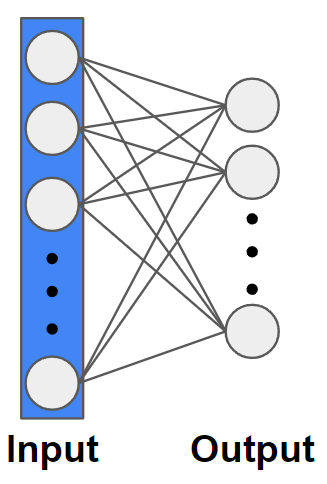
\includegraphics[scale = 0.55]{figs/FFNN.png}
    \caption{Exemplo de FFNN. A camada de entrada na esquerda propaga a informação para a direita (camada de saída). Todos os neurônios entre camadas estão conectados entre si.}
    \label{fig:FFNN}
\end{figure}

\subsubsection*{Convolutional Neural Network}

\par Uma variante da FFNN é a chamada de rede neural convolucional, \textit{Convolutional Neural Network} (CNN). Essa rede consiste em utilizar duas funções convoluídas.
\par A convolução de uma função $f(t)$ por uma função $g(t)$ é dada por $(f*g)(t)$ e definida como: 

%Do ponto de vista matemático sobre convoluções, a convolução descrita como $(f*g)(t)$ de uma função $f(t)$ e outra $g(t)$ é definida como:

\begin{equation}\label{eq:conv_cont}
    (f*g)(t) \equiv \int^{\infty}_{\infty} f(\tau)g(t - \tau)d\tau.
\end{equation}

Para o caso discreto, com $g$ sendo uma função resposta finita de tamanho $2M$ ($M$ é um valor inteiro maior que zero), temos

\begin{equation}\label{eq:conv_disc}
    (f*g)[n] = \sum^{M}_{m = -M} f[n - m]g[m]. 
\end{equation}

\par Convoluções são invariantes sobre operações de rotação e translação, portanto são muito utilizadas para processamento de sinais e imagens \cite{signal_book}. Além disso, a convolução pode ser aplicada de forma discretizada sobre um vetor, se transformando numa forma de filtro. Para ilustrar o que significa isso, no caso discreto e unidimensional, a figura \ref{fig:conv_valid} mostra o processo de convolução de um vetor de tamanho 9 com um filtro de tamanho 3.

\begin{figure}[H]
    \centering
    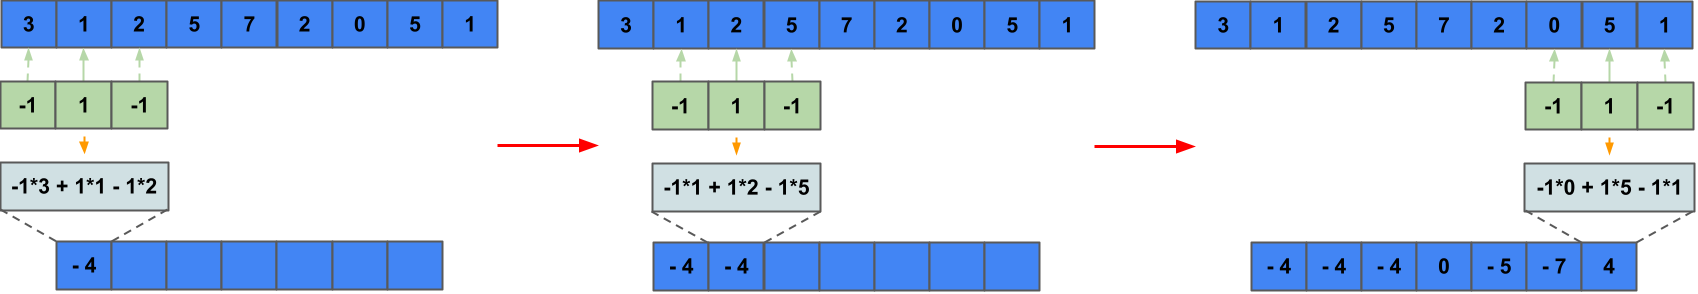
\includegraphics[scale = 0.38]{figs/conv_valid.png}
    \caption{Processo de convolução entre sinal azul em cima e o filtro em verde, resultando no sinal azul embaixo. A multiplicação é feita ponto a ponto e está indicada na caixa azul-clara.}
    \label{fig:conv_valid}
\end{figure}

\par Percebe-se que o sinal resultante tem dimensão menor que o sinal original. O filtro (também chamado de \textit{kernel}) atua em pontos que possuam vizinhos tais que o filtro possa fazer a multiplicação ponto a ponto. Esse tipo de convolução tem o que chamamos de preenchimento válido ou em inglês ``\textit{valid padding}". O tamanho $n_2$ resultante do vetor de saída é 
\begin{equation}
    n_2 = n_1 - m + 1,
\end{equation}
%
onde $n_1$ é o tamanho do vetor de entrada e $m$ o tamanho do filtro (\textit{kernel size}). Uma alternativa para que o vetor de saída tenha o mesmo tamanho do vetor de entrada é acrescentar zeros em torno da entrada, de forma que o vetor de saída tenha o mesmo tamanho que o vetor de entrada. Nesse caso dizemos que o preenchimento é o mesmo ou ``\textit{same padding}". A figura \ref{fig:conv_same} ilustra esse processo.

\begin{figure}[H]
    \centering
    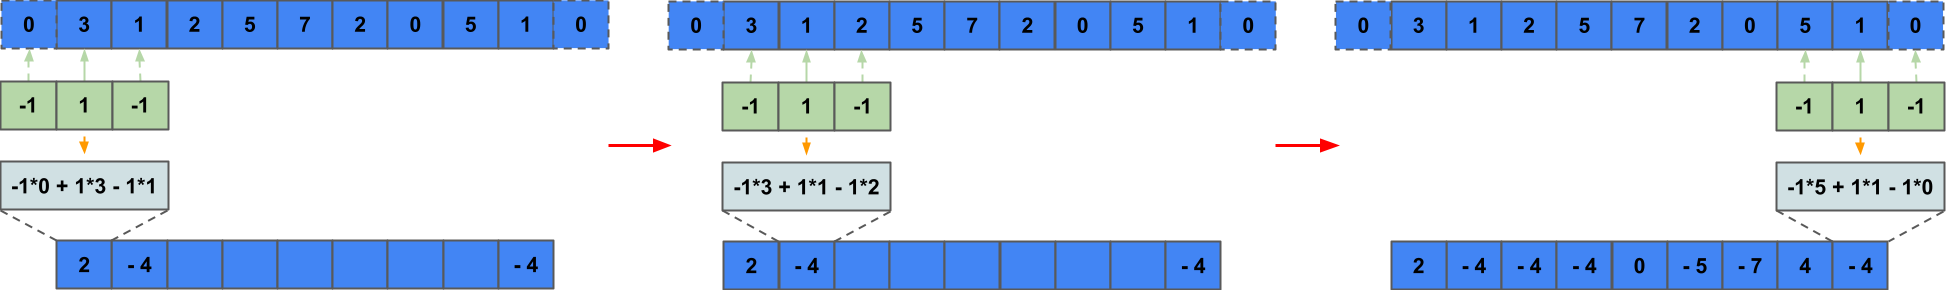
\includegraphics[scale = 0.38]{figs/conv_same.png}
    \caption{Processo de convolução entre o sinal azul em cima e o filtro em verde, resultando no sinal azul embaixo. Agora são acrescentados zeros no inicio e no final do vetor para que o vetor saída tenha o mesmo tamanho do vetor de entrada (nesse caso 9).}
    \label{fig:conv_same}
\end{figure}
%Uma CNN é capaz de fazer convoluções.

%\par Como estamos no contexto de machine learning (inteligência artificial), a priori não sabemos quais os valores dos filtros que devem ser aplicados, apenas seus tamanhos e como agem. A ideia é estimar os valores do filtro (através do treino da rede neural) que deve ser aplicado para se obter o resultado desejado.

\par No contexto de machine learning, não sabemos, a priori, quais os valores dos filtros devem ser utilizados. Temos informações apenas de seus tamanhos e como devem agir. No entanto, podemos estimar os valores dos filtros através do treino da rede neural, para obter o resultado final. Esse treino fornece então os valores dos filtros a serem aplicados que forneçam o resultado esperado.  

\par Cada filtro aplicado gera um mapa característico (\textit{feature map}), que é o resultado da atuação do filtro em um vetor. Usualmente, em uma CNN se escolhe o tamanho do filtro, \textit{padding} (\textit{valid} ou \textit{same}) e quantos filtros serão aplicados (para saber quantos mapas característicos serão gerados). Como temos vários mapas gerados pelos filtros (um por filtro), isso acarreta em um aumento de dimensionalidade. Para selecionar (ou filtrar) os mapas são utilizados critérios, como por exemplo o de selecionar valores máximos dos mapas gerados dada uma janela de atuação, ou seja, de quantos mapas serão comparados para a seleção do valor máximo. O Max-Pooling\footnote{O Max-Pooling máximo é um processo de discretização baseado em amostras. O objetivo é reduzir a amostragem de uma representação de entrada, selecionando amostras pelos seus valores máximos.} faz isso, selecionando valores máximos para uma determinada quantidade de mapas sendo comparados (\textit{pool size}).

% Os filtros têm seus valores estimados pelo treino da rede neural, gerando vários mapas (\textit{feature maps}).

\par Existem disponíveis na literatura várias outras arquiteturas de redes neurais que não serão discutidas aqui. Uma descrição dessas arquiteturas podem ser encontradas nas referências \cite{rbfbook, RNN_fund}.

\section{Estrutura da rede neural}

\par Em nosso trabalho vamos utilizar redes neurais supervisionadas, que serão discutidas em mais detalhes nas próximas seções. Mas de uma forma geral, para a construção de uma rede neural é preciso definir sua estrutura. A estrutura da rede neural possui camadas e cada camada pode possuir uma função de ativação. No geral, tanto a camada de entrada quanto a de saída possuem dimensão fixa. Para cada camada da arquitetura devemos escolher sua função de ativação que dependem dos parâmetros escolhidos. Tanto FFNNs quanto CNNs podem possuir funções de ativação (função $f$ da equação \ref{eq:model_n}) para melhorar o treino com dados que não possuem uma dependência linear. Dentre muitas funções de ativação podemos citar a \textit{Rectified Linear Units} (ReLU)\cite{RELU}, sigmoide \cite{sigmoid_act}, linear e tangente hiperbólica \cite{act_comp}. A figura \ref{fig:ativacoes} mostra os gráficos dessas funções de ativação, onde no eixo x é o argumento e no eixo y o resultado da função.
%\par Para a construção de uma rede neural , precisamos primeiro entender sobre os dados que estamos trabalhando. Grande parte das redes neurais possuem um \textit{input} que deve ter dimensão fixa. O mesmo vale para o \textit{output}.
\begin{figure}[H]
    \centering
    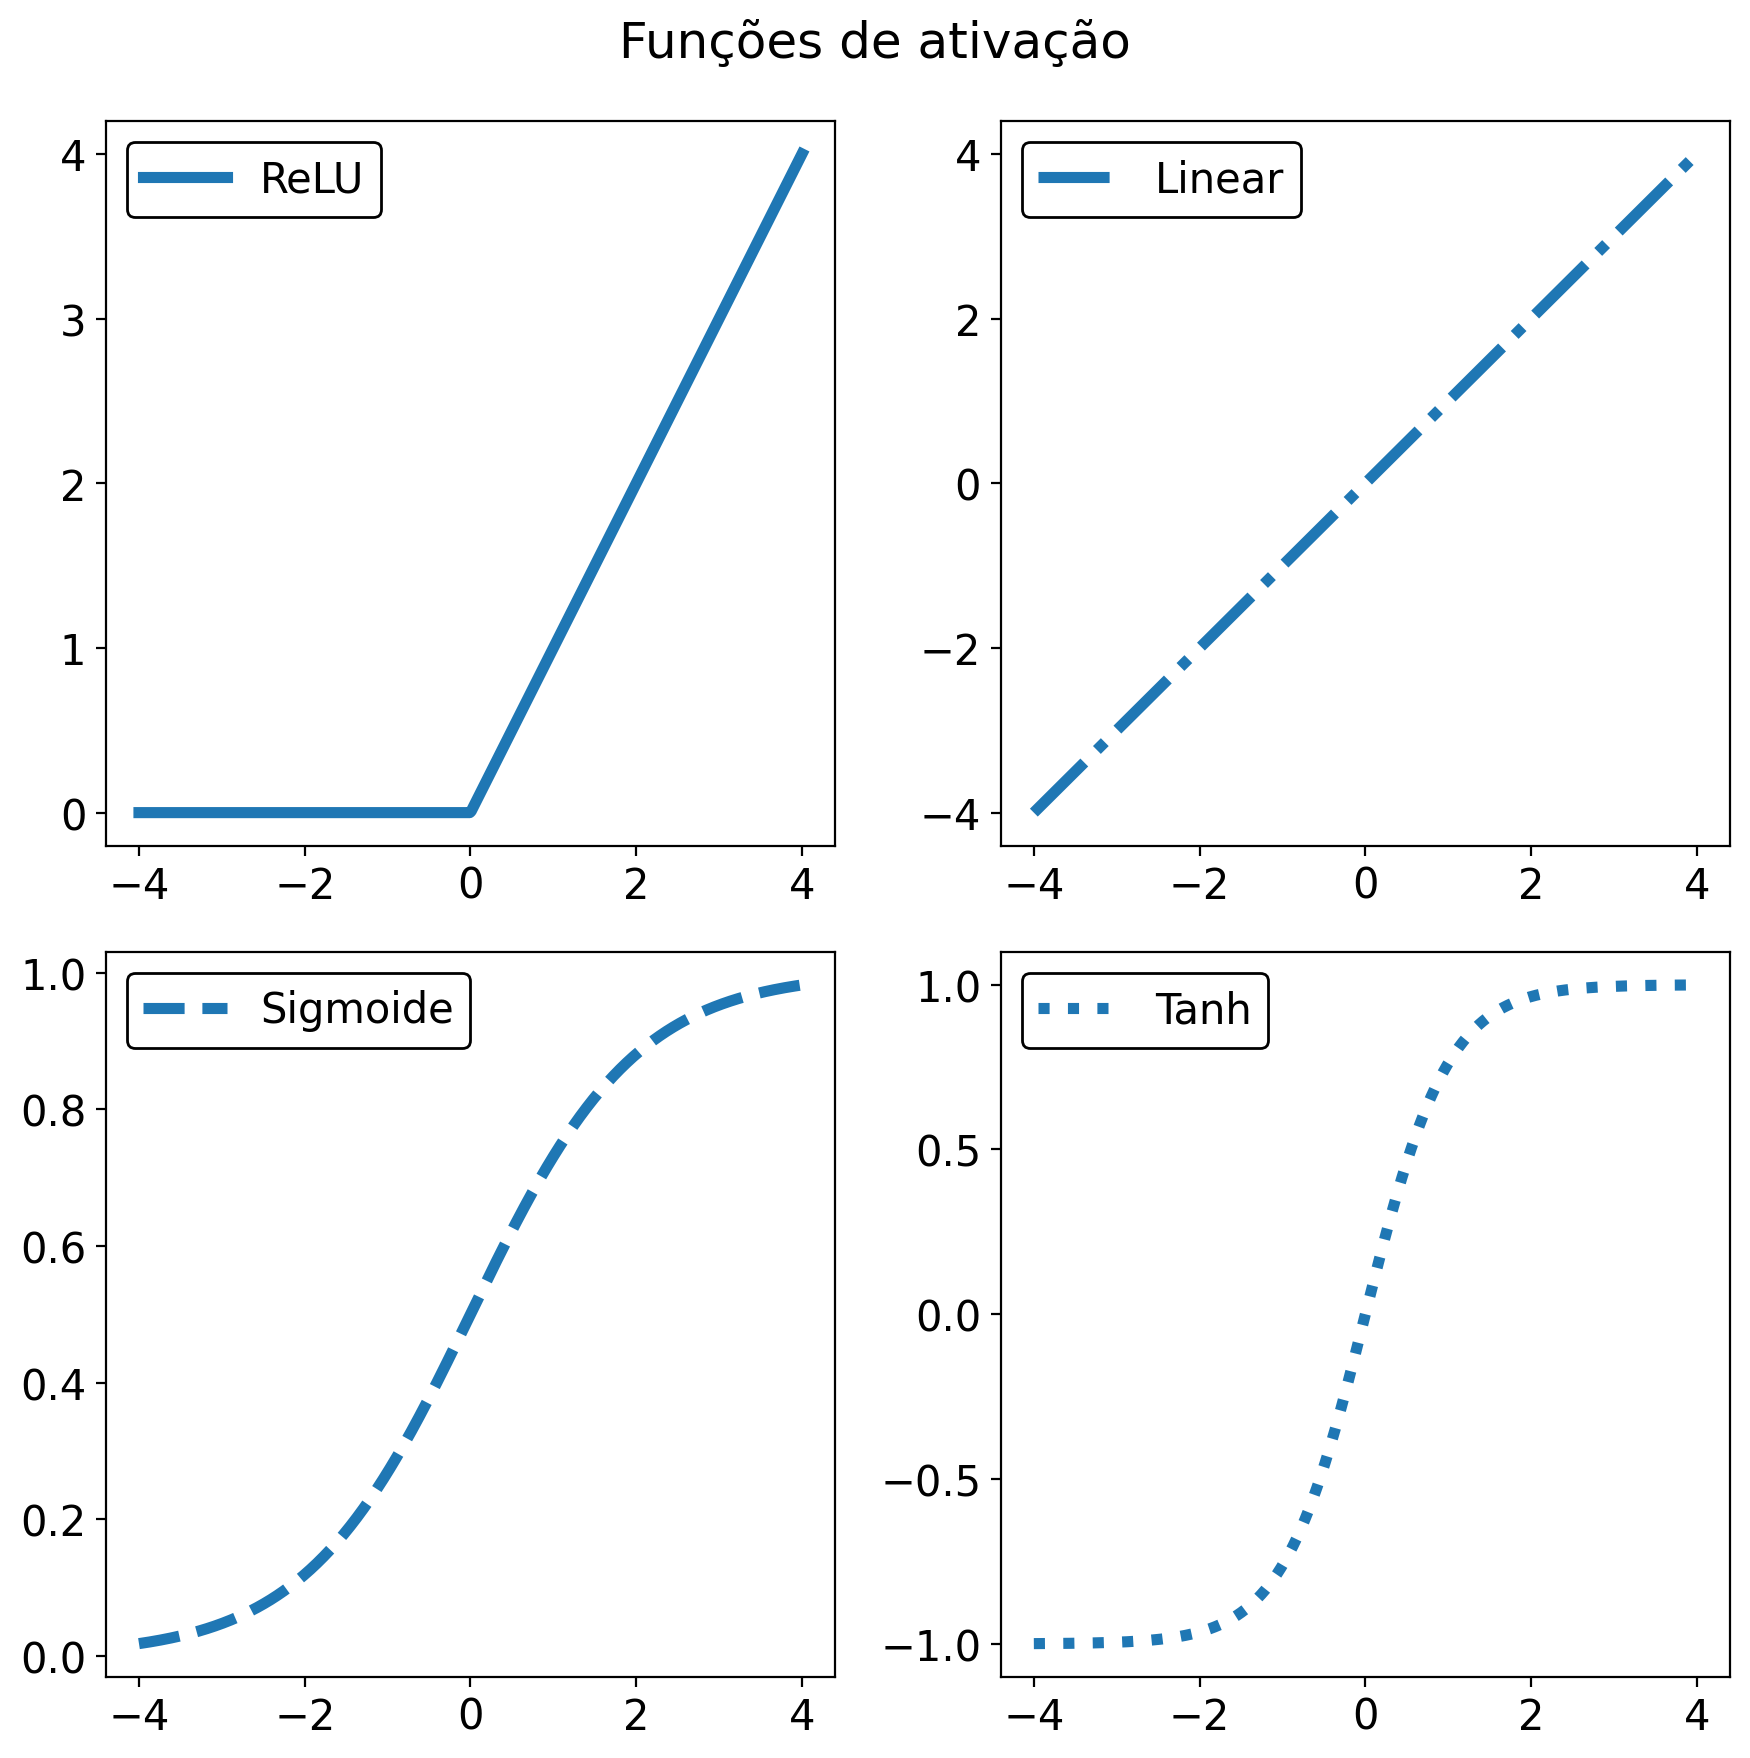
\includegraphics[width=0.8\columnwidth]{figs/ativacoes.png}
    \caption{Funções de ativação e seus respectivos gráficos.}
    \label{fig:ativacoes}
\end{figure}

\par O próximo passo é definir funções corretivas chamadas função custo (algumas vezes também chamada de função \textit{loss}) e o otimizador. A função custo tem o papel de retornar valores altos para previsões erradas e valores baixos para previsões corretas. Por exemplo, se queremos treinar uma rede neural para classificação binária (que prevê duas saídas possíveis), devemos usar a função custo chamada de \textit{binary cross-entropy} dada por \cite{dl_book}

\begin{equation}\label{eq:binary_cross_entropy}
    C(p(y_i)) = -\frac{1}{N}\sum_{i = 1} ^N y_i \log(p(y_i)) + (1 - y_i)\log(1 - p(y_i)),
\end{equation}
%
onde $y_i$ é o rótulo (\textit{label}), $p(y_i)$ é a probabilidade do ponto $y_i$ ser 1 e $N$ é o número de pontos. O objetivo da rede neural é achar o mínimo da função $C(p(y_i))$, o que implica diretamente na melhor solução para o conjunto de dados. Isso é feito pelo método de retropropagação do erro (\textit{backpropagation} \cite{backpropagation}) por um otimizador. Outros exemplos de função custo são o erro quadrático médio ou \textit{categorical cross-entropy} \cite{MSE_CEF_review}.

\par O otimizador, por sua vez, tem o objetivo de otimizar os parâmetros presentes na rede neural, buscando o mínimo global da função custo, o que nem sempre acontece, pois a minimização pode parar em um mínimo local da função. Existem diversos otimizadores disponíveis na literatura, como por exemplo o \textit{Stochastic Gradient Descent} (SGD), \textit{Adaptive Moment Estimation} (ADAM), ADAMAX \cite{ADAMAX}, entre outros \cite{gradient_over}. Por exemplo, para o SGD, temos que a atualização de parâmetros é dada por

\begin{equation}\label{eq:SGD}
    \theta_j = \theta_{j} - \alpha \frac{\partial }{\partial \theta_j}C(\theta),
\end{equation}
%
onde $\theta_j$ é o parâmetro a ser atualizado, $\alpha$ é a taxa de aprendizado (\textit{learning rate}) e $C(\theta)$ é a função custo que depende dos parâmetros $\theta$.

\par Para enfim treinar a rede neural, devemos escolher o tamanho das amostras (\textit{batch size}) que será usada para o treino, por iteração em cada rodada de treino. Por exemplo, se usamos 1000 observações para o treino, e o \textit{batch size} é 500, cada rodada de treino terá duas iterações. No geral, usamos \textit{batch sizes} pequenos, pois o consumo de memória é mais eficiente.

\par Para avaliação da rede neural devemos ainda utilizar dados de validação, que servem para verificar o comportamento da rede neural que está sendo treinada. Esse conjunto de dados usados não é usado para o treino, são usados apenas para verificar possíveis problemas como o \textit{overfit}. O \textit{overfit} ocorre quando a rede neural começa a se adequar perfeitamente aos dados de treino, perdendo a capacidade de previsão em dados que não estão sendo usados no treino pela rede neural.

\par Além dos dados de validação, podemos escolher métricas que auxiliam a visualização do comportamento da rede neural durante o treino e nos retornam informações importantes sobre sua qualidade. Exemplos importantes de métricas são: acurácia binária, erro médio absoluto e acurácia categórica \cite{metrics}. Por exemplo, caso seja necessário verificar se uma rede neural está fazendo previsões certas em um problema cuja classificação é binária, então a métrica deve ser a acurácia binária. Tudo depende do objetivo da rede neural. Em nosso trabalho utilizamos o erro médio absoluto e acurácia binária.

\section{Sistemas de \textit{machine learning}}

\par As redes neurais e os procedimentos de validação e treino formam os sistemas de machine learning. Podemos dividir os sistemas de machine learning em quatro tipos:

\subsubsection*{Aprendizado Supervisionado}
% \begin{enumerate}
%     \item aprendizado supervisionado;
%     \item aprendizado não supervisionado;
%     \item aprendizado semi supervisionado;
%     \item aprendizado por reforço.
% \end{enumerate}

\par Aprendizado supervisionado é quando fornecemos para a rede neural um conjunto de dados para o treino com a solução desejada (chamados de \textit{labels}). Um uso típico desse tipo de sistema é para problemas de classificação de imagens (identificação de figuras), previsão de valores numéricos etc \cite{mlbook}. Exemplos de algoritmos supervisionados são:

\begin{itemize}
    \item \textit{k-Nearest Neighbors} (é necessário saber o número de aglomerados a priori) \cite{knn}
    \item Regressão linear
    \item \textit{Support Vector Machines} (SVMs)
    \item \textit{Decision Trees} e \textit{Random Forests}
    \item Redes neurais
\end{itemize}

\subsubsection*{Aprendizado não supervisionado}

\par Aprendizado não supervisionado é quando fornecemos o conjunto de dados sem rótulos ou características a priori. Nesse caso, o sistema deve aprender a realizar uma determinada tarefa sem supervisão. Um problema comum, por exemplo, é quando queremos identificar aglomerados em um conjunto de dados (\textit{clustering}) \cite{unsupervised, knn_uns}, ou remover ruído com estruturas chamadas \textit{autoencoder}\footnote[1]{\textit{Autoencoder} é uma técnica de aprendizado não supervisionado para redes neurais aprenderem a comprimir e codificar dados de modo eficiente.} \cite{8621080}.

\subsubsection*{Aprendizado semi supervisionado}

\par Temos ainda o aprendizado semi supervisionado, quando apenas parte do conjunto de dados para o treino possui \textit{labels}. Isso é comum quando se obtém conjuntos de dados diferentes e apenas parte deles foi rotulado \cite{semi_supervised}.

\subsubsection*{Aprendizado por reforço}

\par Aprendizado por reforço é quando um sistema, chamado de \textit{agente}, aprende através do ambiente, realizando ações que maximizam sua recompensa. Por exemplo, caso o sistema realize uma ação incorreta, ele recebe uma penalidade, fazendo com que procure outra maneira de realizar a ação, se essa maneira for a correta o sistema é recompensado \cite{reinforcement}. Esse tipo de sistema é muito usado, por exemplo, em automatização robótica, como carros que pilotam sozinhos, robôs que aprendem a andar etc. \cite{robot_ml}

%\section{Aplicações de \textit{machine learning} na física nuclear}

\par Alguns usos recentes de machine learning em física nuclear são apresentados no apêndice \ref{appendix:ml_nuclear}. Em nosso trabalho vamos utilizar técnicas de machine learning para analisar dados de reações nucleares obtidos de medidas com um instrumento específico, alvo ativo.

%\par Com essa breve descrição sobre machine learning e exemplos do seu uso em problemas de física nuclear (apêndica \ref{appendix:ml_nuclear}), pode-se seguir adiante e entender seu uso dentro deste trabalho, que está feito nos próximos capítulos.

\chapter{Reconstrução de nuvens de pontos a partir de algoritmos de \textit{machine learning}}\label{chapter:sinais}

\par Nesse capítulo vamos descrever o procedimento usado para criar as nuvens de pontos (\textit{point clouds}) a partir dos pulsos medidos em cada pixel do micromegas, usando algoritmos de machine learning supervisionado.

\par Algoritmos baseados em CNNs vem sendo usados com relativo sucesso para o processamento e análise de sinais \cite{FORTINO2022166497}, como por exemplo para discriminação de pulsos \cite{Holl2019}. CNNs possuem a capacidade de fazer ajustes multidimensionais e aprender padrões complexos. Além disso, CNNs são mais eficientes em tempo para a análise de grandes quantidades de dados em comparação com algoritmos comuns \cite{FORTINO2022166497}.

\par Para que possamos obter dados de posição, trajetória e energia das partículas nas medidas com alvo ativo precisamos realizar análise dos pulsos medidos. A quantidade de pulsos gerados nesse experimento é da ordem de centenas de milhões. Para a análise completa dos pulsos, são necessárias diferentes etapas que envolvem processos que muitas vezes precisam ser refeitos por causa de algum um erro no processo análise. Notar algum erro no processo, ou ter que mudar algum parâmetro da análise, significaria ter que analisar novamente os dados, sendo um processo muito custoso em tempo.

\par O uso de algoritmos de CNNs tem o objetivo de diminuir o tempo consumido para a análise dos pulsos. As redes neurais criadas são treinadas uma única vez e podem ser utilizadas de modo separado e/ou acoplado \cite{FORTINO2022166497}, como está mostrado na sequencia do capítulo.

\par Os pulsos medidos com o detector micromegas são digitalizados em 512 intervalos de tempo (\textit{time buckets}). A análise desses espectros temporais (evolução do pulso com o tempo) foi dividida em três etapas: correção do fundo, deconvolução do sinal e identificação de picos. As redes neurais criadas foram supervisionadas, o que significa que foi necessário incluir um grande volume de dados rotulados para o algoritmo aprender a lógica da operação. Para isso foi feito um grande banco de dados, utilizado no treinamento das redes neurais, que se beneficiam da grande quantidade de dados usada para o treino \cite{mlbook}. Na seção \ref{sec:pulses_trad}, está mostrado como o banco de dados para o treino das redes neurais desenvolvidas foi criado, e a construção das redes neurais está na seção \ref{sec:pulsos_ml}.


% os sinais foram analisados a partir de métodos mais tradicionais e depois criando algoritmos de \textit{machine learning}, usando das soluções anteriores como base para o seu funcionamento.


% \par A quantidade de histogramas armazenados ultrapassa facilmente a casa das centenas de milhões, portanto é necessário o desenvolvimento de algoritmos extremamente rápidos para a análise.


\section{Construção do banco de dados para as redes neurais}\label{sec:pulses_trad}

\par Cada um dos pixels do detector micromegas possui uma eletrônica independente que gera pulsos digitais como os mostrados na \ref{fig:exemplos_sinais}. Centenas de sinais como esses são produzidas em cada um dos eventos.

\begin{figure}[H]
\centering
    \begin{subfigure}[b]{0.48\textwidth}
        \centering
        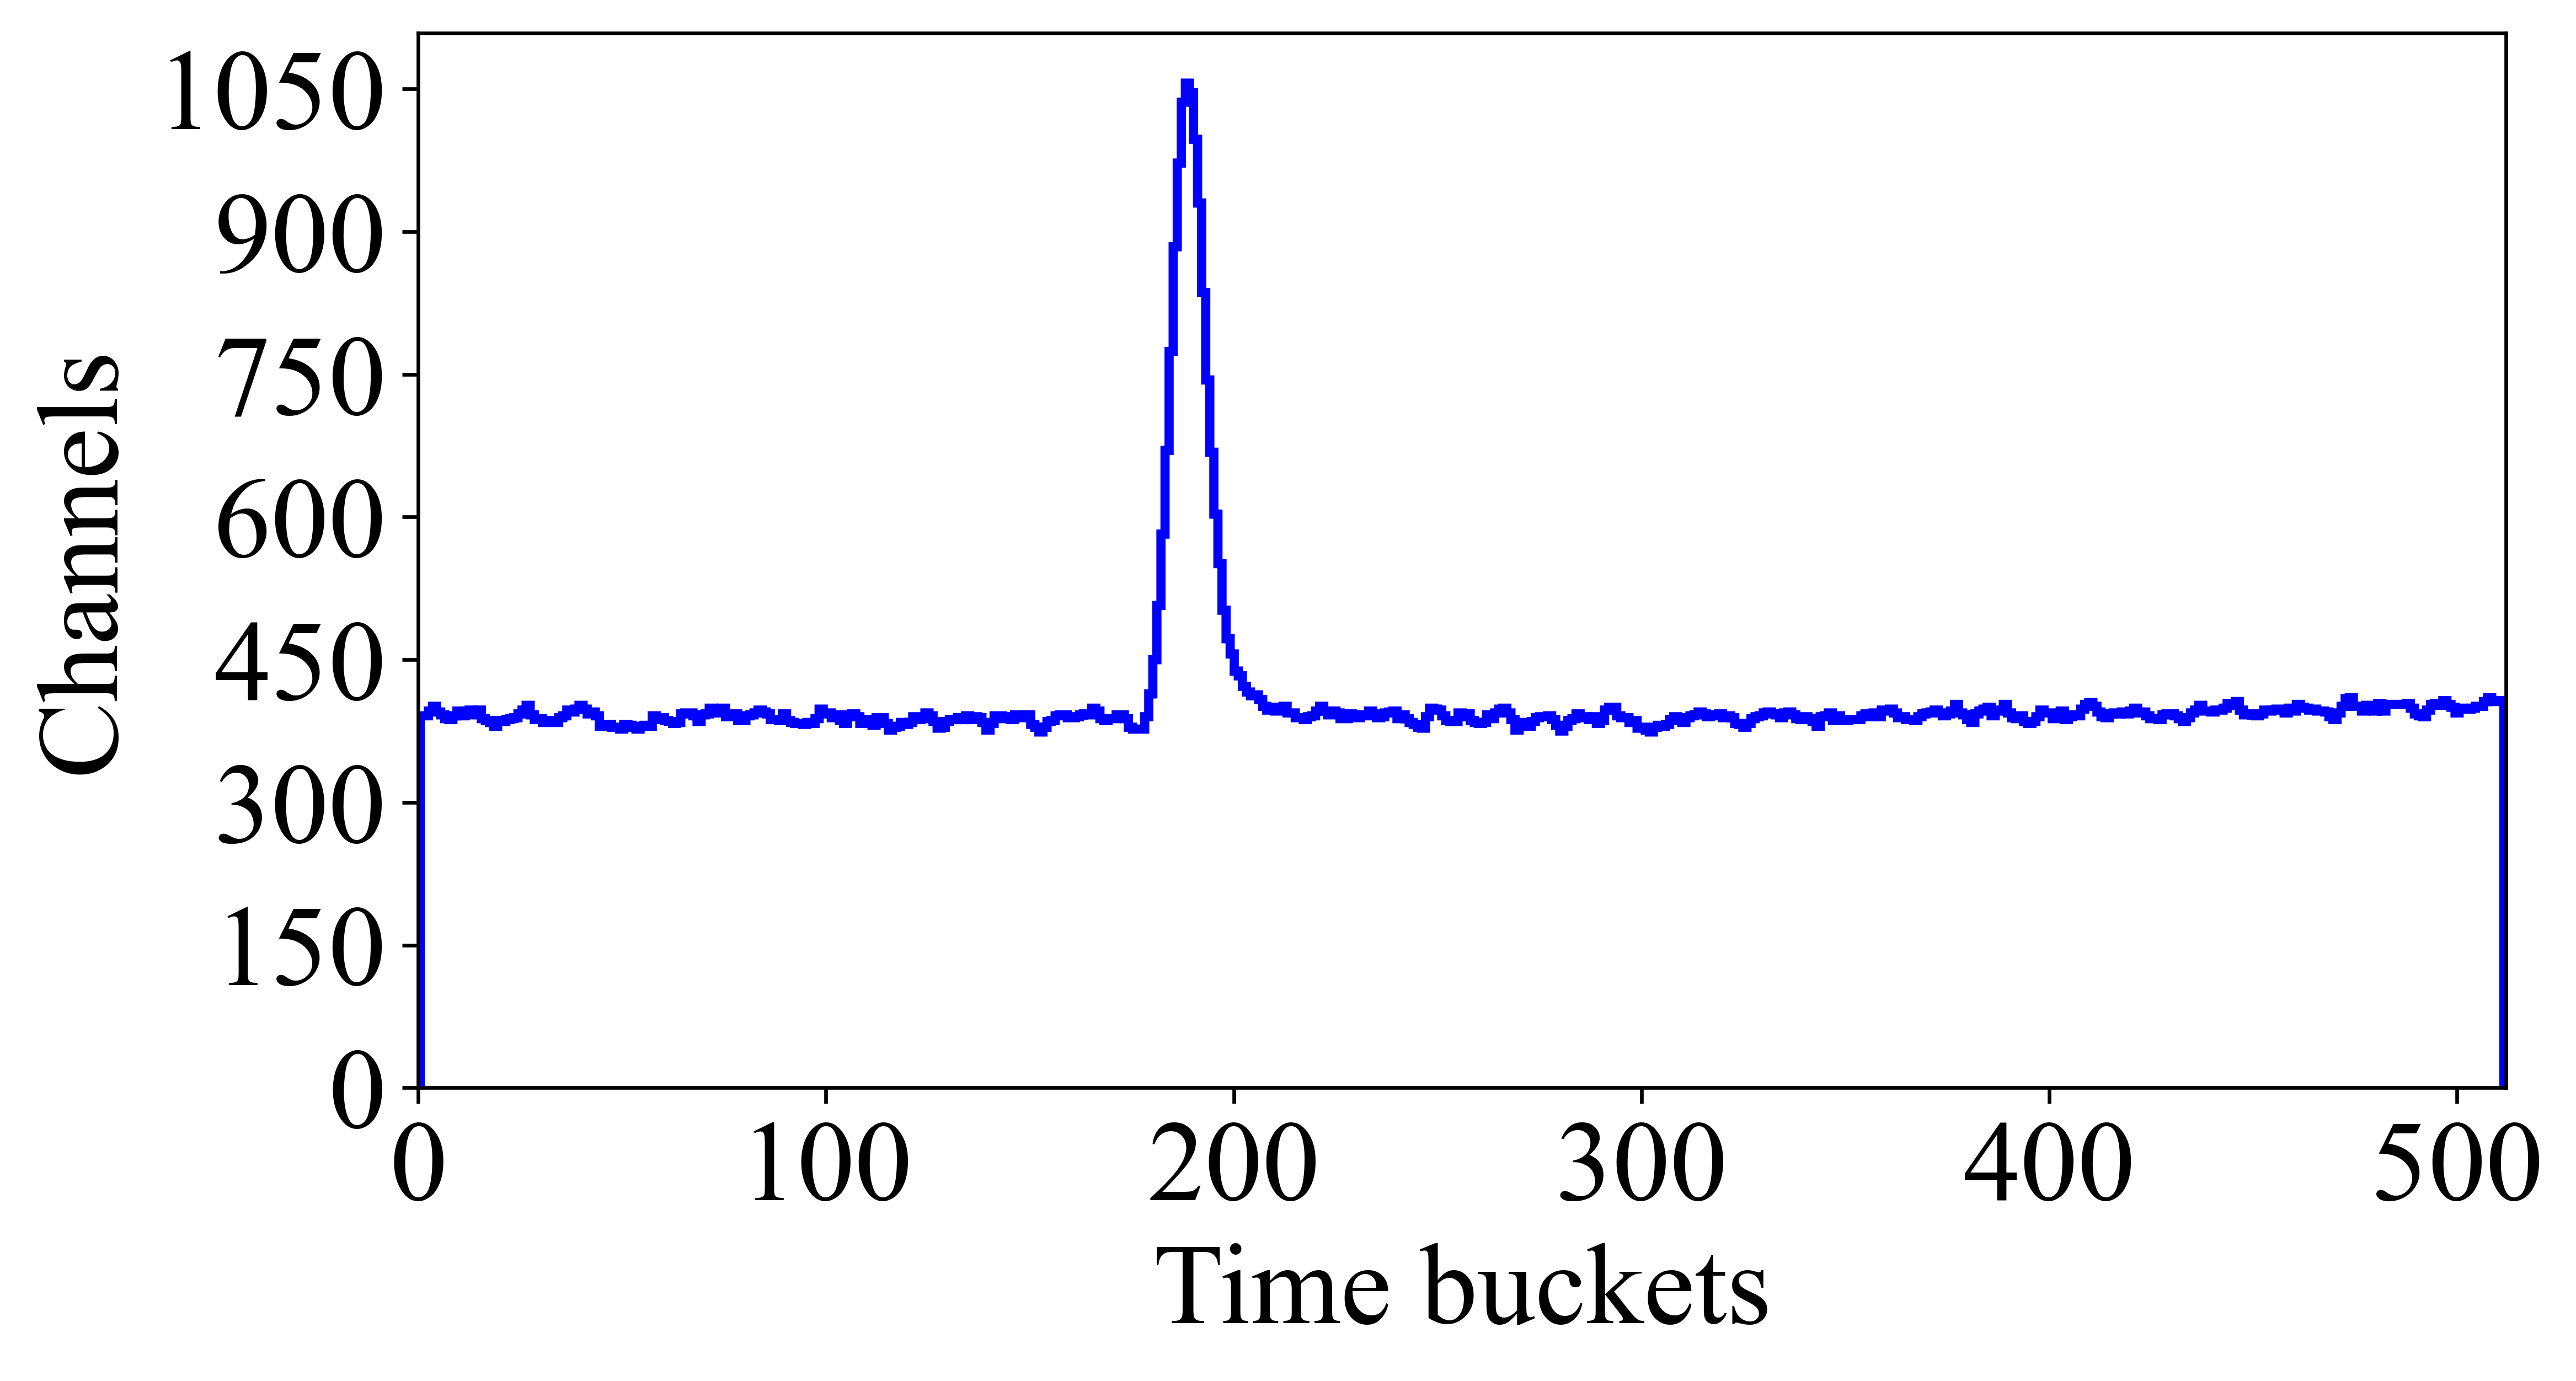
\includegraphics[scale=0.395]{figs/ex_sinal_1.png}
        \caption{}
        \label{subfig:exemplos_sinais_1}
    \end{subfigure}%
    \hfill
    \begin{subfigure}[b]{0.48\textwidth}
        \centering
        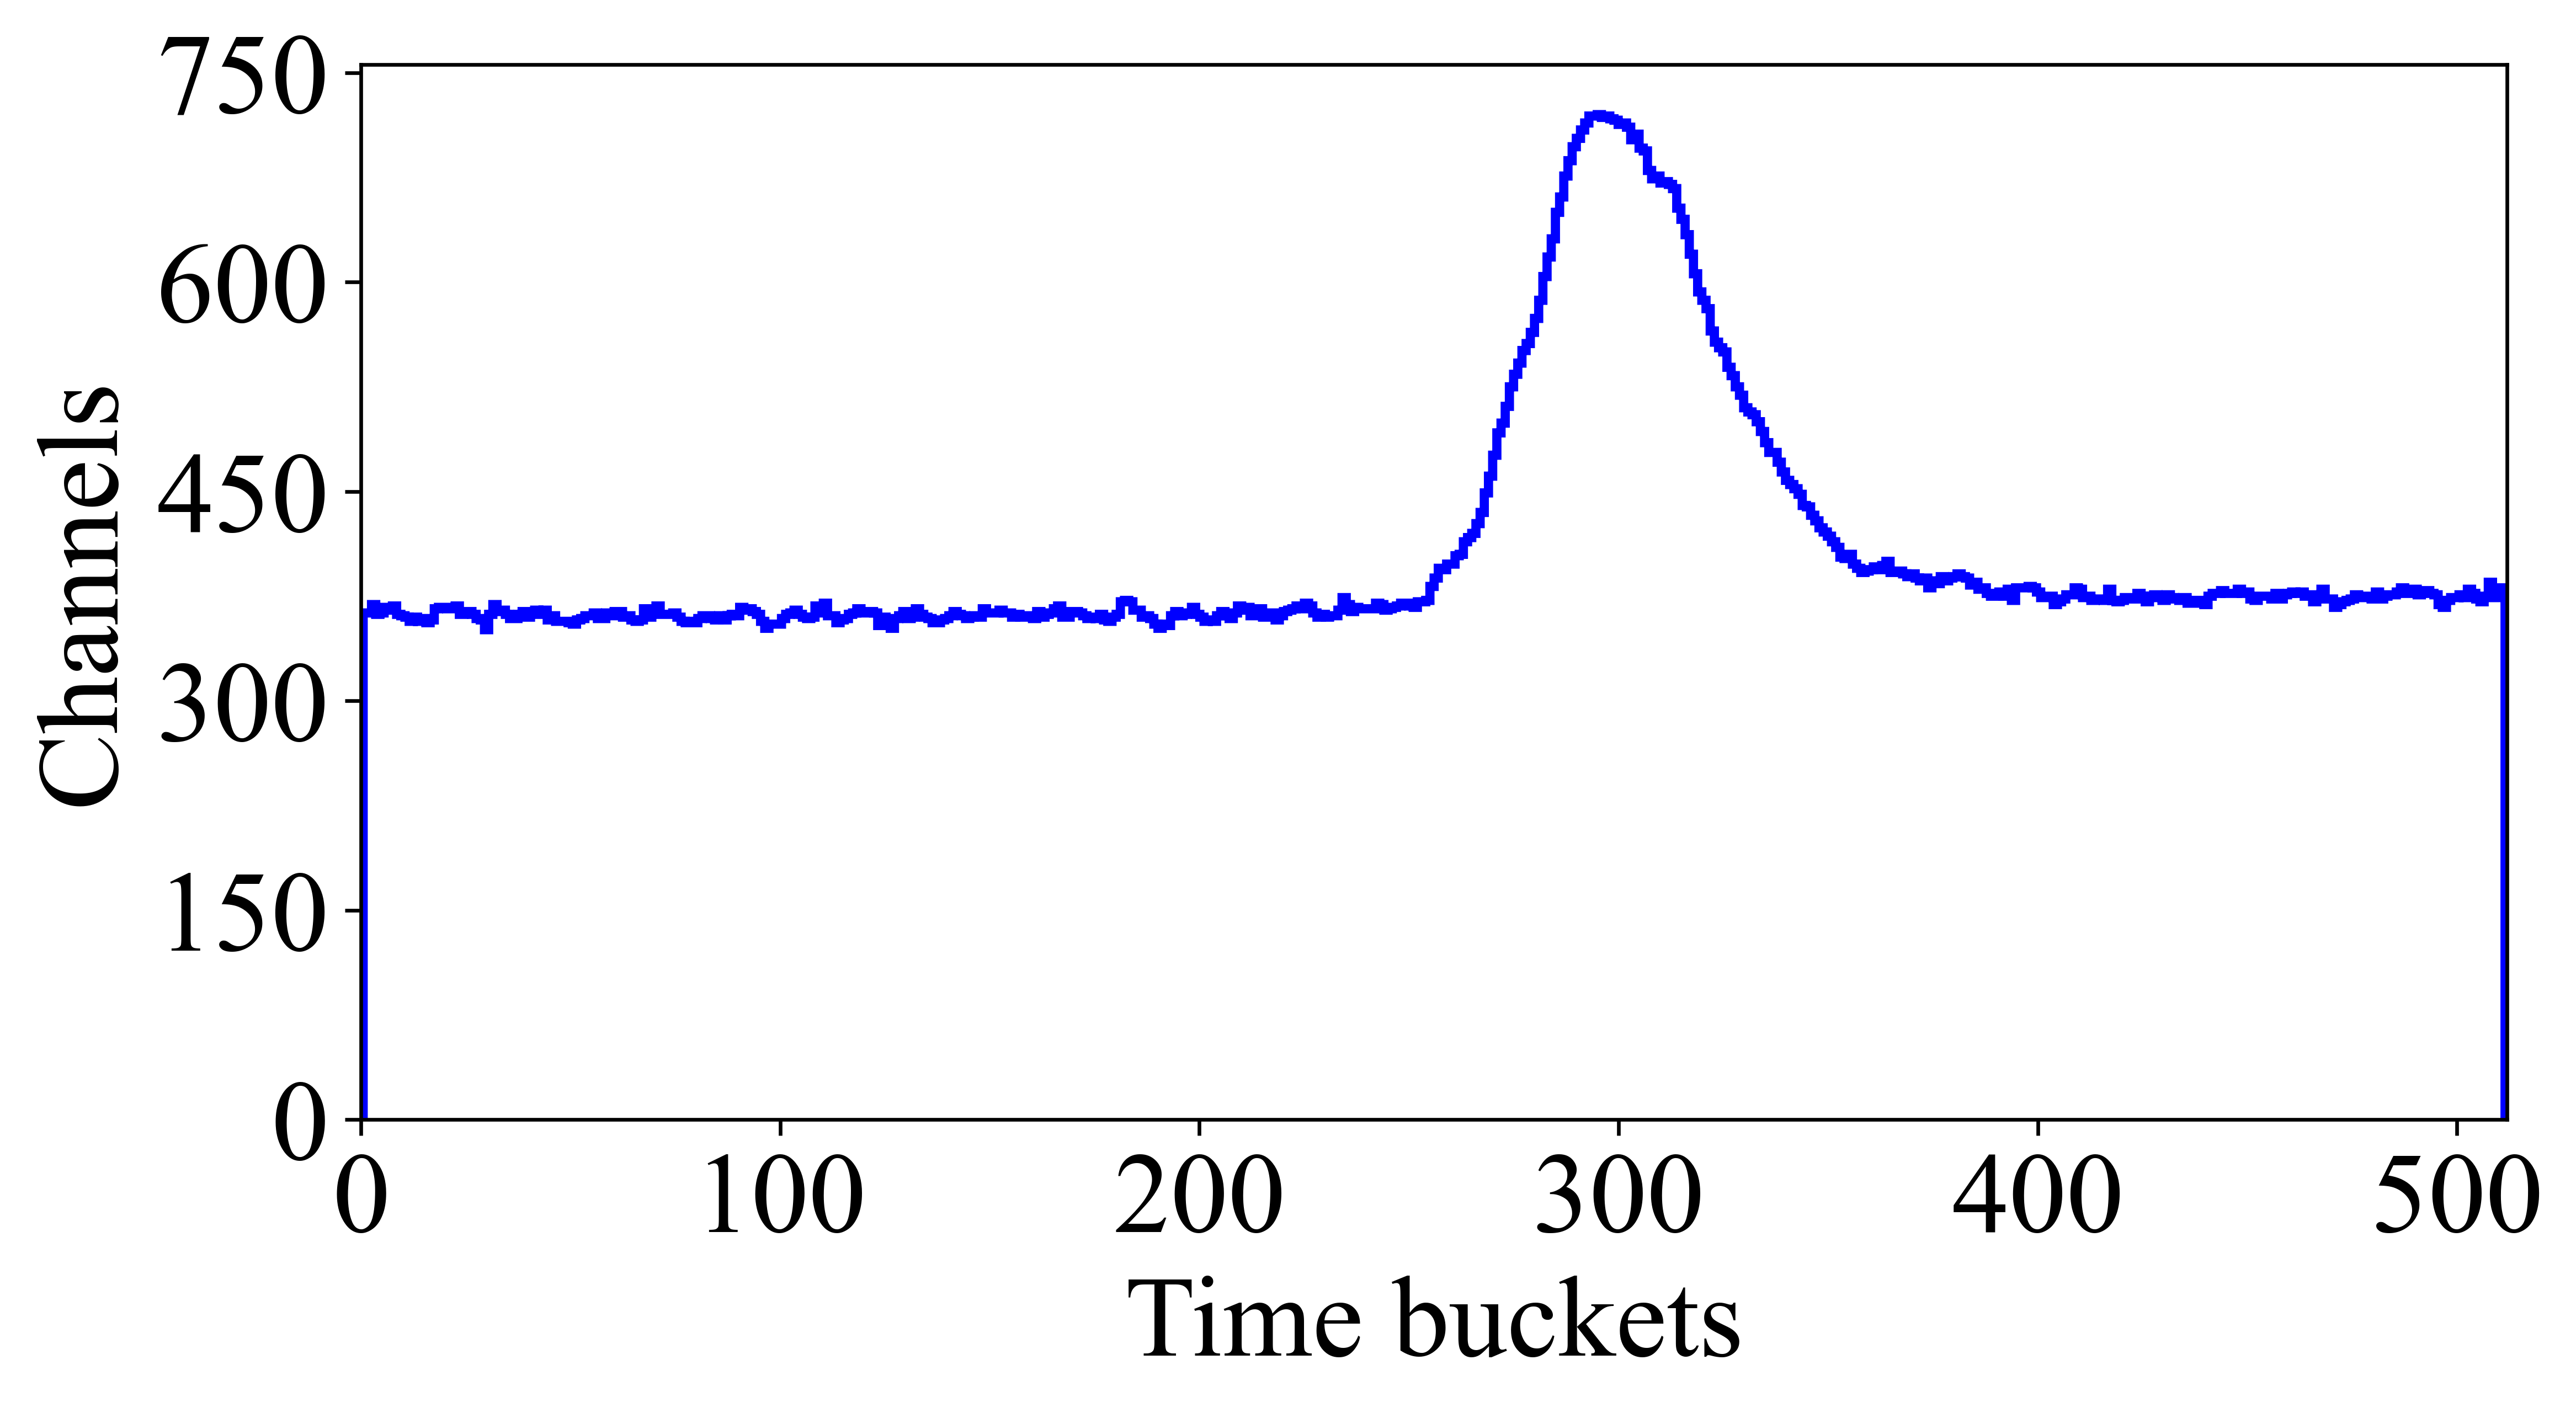
\includegraphics[scale=0.395]{figs/ex_sinal_2.png}
        \caption{}
        \label{subfig:exemplos_sinais_2}
    \end{subfigure}
\caption{Exemplos de sinais produzidos pelos canais do detector. Em \ref{subfig:exemplos_sinais_1} o sinal possui apenas um pulso, enquanto em \ref{subfig:exemplos_sinais_2} há vários pulsos em sobreposição, formando um único pulso com largura maior que em \ref{subfig:exemplos_sinais_1}.}
\label{fig:exemplos_sinais}
\end{figure}

\par Na figura \ref{fig:exemplos_sinais}, o eixo $x$ corresponde à cada um dos 512 \textit{time buckets} possui largura de cerca de 115 ns. No eixo $y$ tem-se o canal de ADC para cada time bucket. Na figura \ref{subfig:exemplos_sinais_1} há um sinal com um pedestal (fundo ou \textit{baseline}) com altura entre 300 e 450 canais, e um pulso estreito em cima. O fundo está composto por ruído de alta e baixa frequência, o que geralmente dificulta o ajuste com uma função analítica. Como mostrado na seção \ref{PATTPC}, os elétrons que surgiram da ionização do gás foram conduzidos perpendicularmente pelo campo elétrico até o detector. A interação da partícula com o gás é evidenciada justamente pelo pulso presente em \ref{subfig:exemplos_sinais_1}. O centroide de cada pulso está relacionado ao tempo de deriva dos elétrons (em unidade de time buckets) que é usado para determinar a coordenada $z$ da interação da partícula com o gás. A energia depositada no gás é obtida a partir da área do pulso sem fundo.

%Cada pixel $i$ do detector está em uma posição ($x_i$, $y_i$), o centroide de cada gaussiana fornece a coordenada em $t$ (\textit{time bucket}) para então ser convertida na posição em coordenada $z$ do ponto de interação da partícula com o gás, e a energia depositada $Q$ é obtida da área do pulso sem fundo (gaussiana com centroide $t$).

\par Para a figura \ref{subfig:exemplos_sinais_1} tem-se apenas um pulso estreito, o que corresponde à uma partícula incidindo paralelamente ao plano do detector (perpendicular ao campo elétrico). No caso da figura \ref{subfig:exemplos_sinais_2}, há uma distribuição ampla do sinal do tempo, o que corresponde à uma partícula incidindo quase perpendicularmente ao plano do detector. A ilustração desse processo está na figura \ref{fig:get_signal}, que mostra que o sinal resposta do processo de passagem de uma partícula carregada no gás depende do ângulo relativo ao plano de projeção. Trajetórias paralelas ao plano de detecção tem distribuição em tempo bem definidas pois a interação corresponde a apenas um ponto no eixo de projeção. Trajetórias perpendiculares ao plano de detecção tem distribuições em tempo mais largas devido a que os elétrons são produzidos numa região mais ampla.


% único pixel do detector ativado com coordenadas($x$, $y$, $z$). Já para \ref{subfig:exemplos_sinais_2} temos o que é chamado de mistura de gaussianas (\textit{gaussian mixture}), que é a presença de várias gaussianas sobrepostas. Esse tipo de sinal corresponde ao feixe indo perpendicularmente ao pixel do plano do detector, indicando. A ilustração desse processo está na figura \ref{fig:get_signal}, que mostra o processo da passagem de uma partícula carregada e como o sinal é gerado a partir disso.

% As gaussianas presentes em \ref{subfig:exemplos_sinais_2} devem ter a mesma largura da gaussiana presente em \ref{subfig:exemplos_sinais_1}. 

\begin{figure}[H]
    \centering
    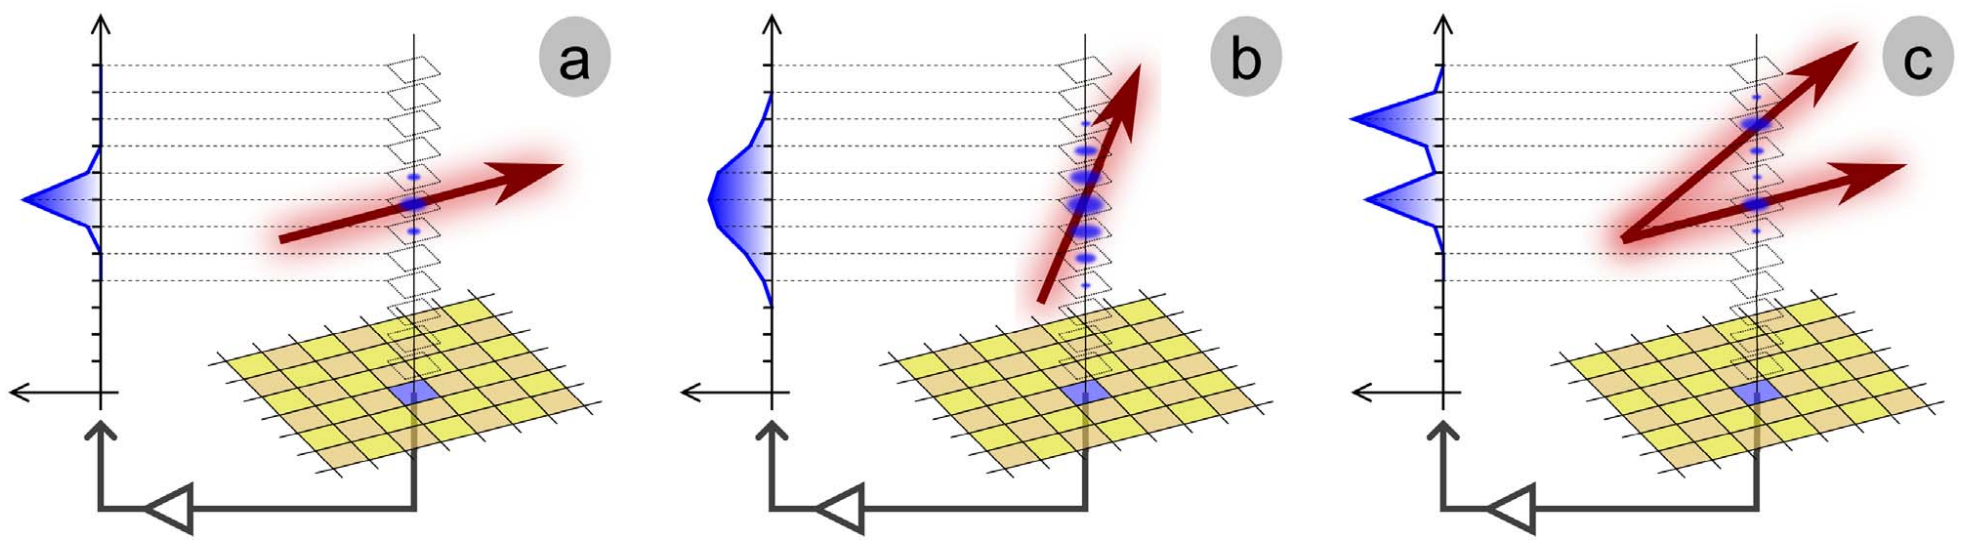
\includegraphics[scale = 0.29]{figs/get.png}
    \caption{Ilustração que mostra a variação no formato da carga coletada a partir da passagem de uma partícula carregada dentro do TPC, onde o plano do detector está embaixo. No lado esquerdo de cada imagem, a distribuição do sinal coletado por um único pad (escuro) do plano de coleta é mostrado (o canal eletrônico de leitura é representado pela seta cinza em negrito). No caso de uma trajetória quase horizontal em relação ao plano do detector (a), o sinal é uma distribuição estreita, enquanto para uma trajetória próxima a uma direção vertical (ou perpendicular) em relação ao detector (b), a distribuição deve ser muito mais ampla (vários pontos de interação da partícula com o gás devem ser extraídos desse sinal). A última imagem ilustra o caso em mais de uma trajetória de partículas contribui para o sinal \cite{GET}.}
    \label{fig:get_signal}
\end{figure}

\par Para analisar os pulsos deve-se primeiro remover o fundo (pedestal ou baseline) dos sinais. O sinal de fundo é complexo e pode variar em função do canal e também por evento. O sinal pode ser alterado por flutuações causadas pelo circuito eletrônico e por efeitos sistemáticos gerados pela memória de buffer circular, podendo o tornar não analítico \cite{FORTINO2022166497, GET}. Após a eliminação do fundo, os sinais foram tratados realizando uma deconvolução, aumentando a resolução dos pico em várias gaussianas com centróides que correspondem a informação temporal do sinal. Essas gaussianas são então usadas para a reconstrução da nuvem de pontos da trajetória das partículas no alvo gasoso. Todo esse processo foi realizado nesse trabalho com algoritmos de machine learning supervisionado que desenvolvemos \cite{FORTINO2022166497}. Para isso, foi criado um banco de dados que serviu de saída e/ou entrada para o treino das redes neurais. O processo de criação dos dados para o treino das redes neurais está descrito nas ssubseções \ref{subsec:pulses_baseline} e \ref{subsec:pulses_deconv}, enquanto o processo de criação das redes neurais é descrito na seção \ref{sec:pulsos_ml}. 

% O fundo não é trivial de se determinar, pois não é analítico, oscilando muito entre os canais.

\subsection{Estimativa do fundo}\label{subsec:pulses_baseline}

\par Para que pudéssemos realizar a análise dos pulsos temporais, era necessário a eliminação do fundo. A primeira tentativa para estimarmos o sinal sem o fundo foi desenvolvida utilizando-se uma transformada de Fourier e um filtro passa-baixa, que nada mais é do que a função resposta do detector fornecida na Ref. \cite{GET}. Para explicarmos o procedimento, vamos primeiramente considerar uma função $f(t)$ qualquer, sua transformada de Fourier é dada por

\begin{equation} \label{eq:fourier}
    \hat{f}(\nu)=\mathscr{F}[f(t)]=\int_{-\infty}^{\infty} f(t) e^{-2 \pi i \nu t} d t.
\end{equation}

\par Primeiro calculamos a transformada de Fourier $\hat{f}(\nu)$ do sinal, em seguida o multiplicamos pela função resposta do detector $h(\nu)$ dada por \cite{GET}

\begin{equation}
    h(\nu) = A*\exp\left (\nu \tau \right)\left(\nu \tau\right)^3 \sin \left( \nu \tau \right) ,
\end{equation}
%
onde $A$ está relacionado com o ganho de amplificação e $\tau$ é o tempo de pico (peaking time), que é o tempo de modelagem da cadeia de amplificação \cite{GET}. Do teorema da convolução, temos que \cite{metodos_mat_aplicada}

%\par onde $a$ é um fator de escala. A função sinc foi escolhida para tirar vantagem do Teorema da Convolução, dado por\cite{metodos_mat_aplicada}

\begin{equation}
    \mathscr{F}^{-1}[\hat{f}(\nu) \hat{g}(\nu)]=(f * g)(t)=\int_{-\infty}^{\infty} f(\tau) g(t-\tau) d \tau, 
\end{equation}
%
onde $(f * g)(t)$ é a convolução entre $f(t)$ e $g(t)$. Multiplicar o sinal transformado por $h(\nu)$ e depois inverter inverter a transformação é o mesmo que convoluir o sinal original com a transformação inversa de $h(\nu)$, o que resulta no sinal sem o fundo \cite{josh_bradt, GET}. Resultados desse procedimento estão na figura \ref{fig:bs_fourier_exs}.

%Multiplicar o sinal transformado por $\sinc (\nu / a)$ e depois inverter inverter a transformação é o mesmo que convoluir o sinal original com a transformação inversa de $\sinc (\nu / a)$, pois

%\begin{equation}
%\mathscr{F}^{-1}[\sinc(\nu)]=\rect(t) \equiv \begin{cases}1, & -\frac{1}{2}<t<\frac{1}{2} \\ 0, & \text { qualquer outro }t\end{cases},
%\end{equation}
%
%é uma função que representa uma janela retangular, o que seria um exemplo de função resposta do detector. Caso saibamos essa função resposta, então é possível reconstruir completamente o sinal. Resultados desse procedimento estão na figura \ref{fig:bs_fourier_exs}.

\begin{figure}[H]
\centering
    \begin{subfigure}[c]{0.45\textwidth}
        % \centering
        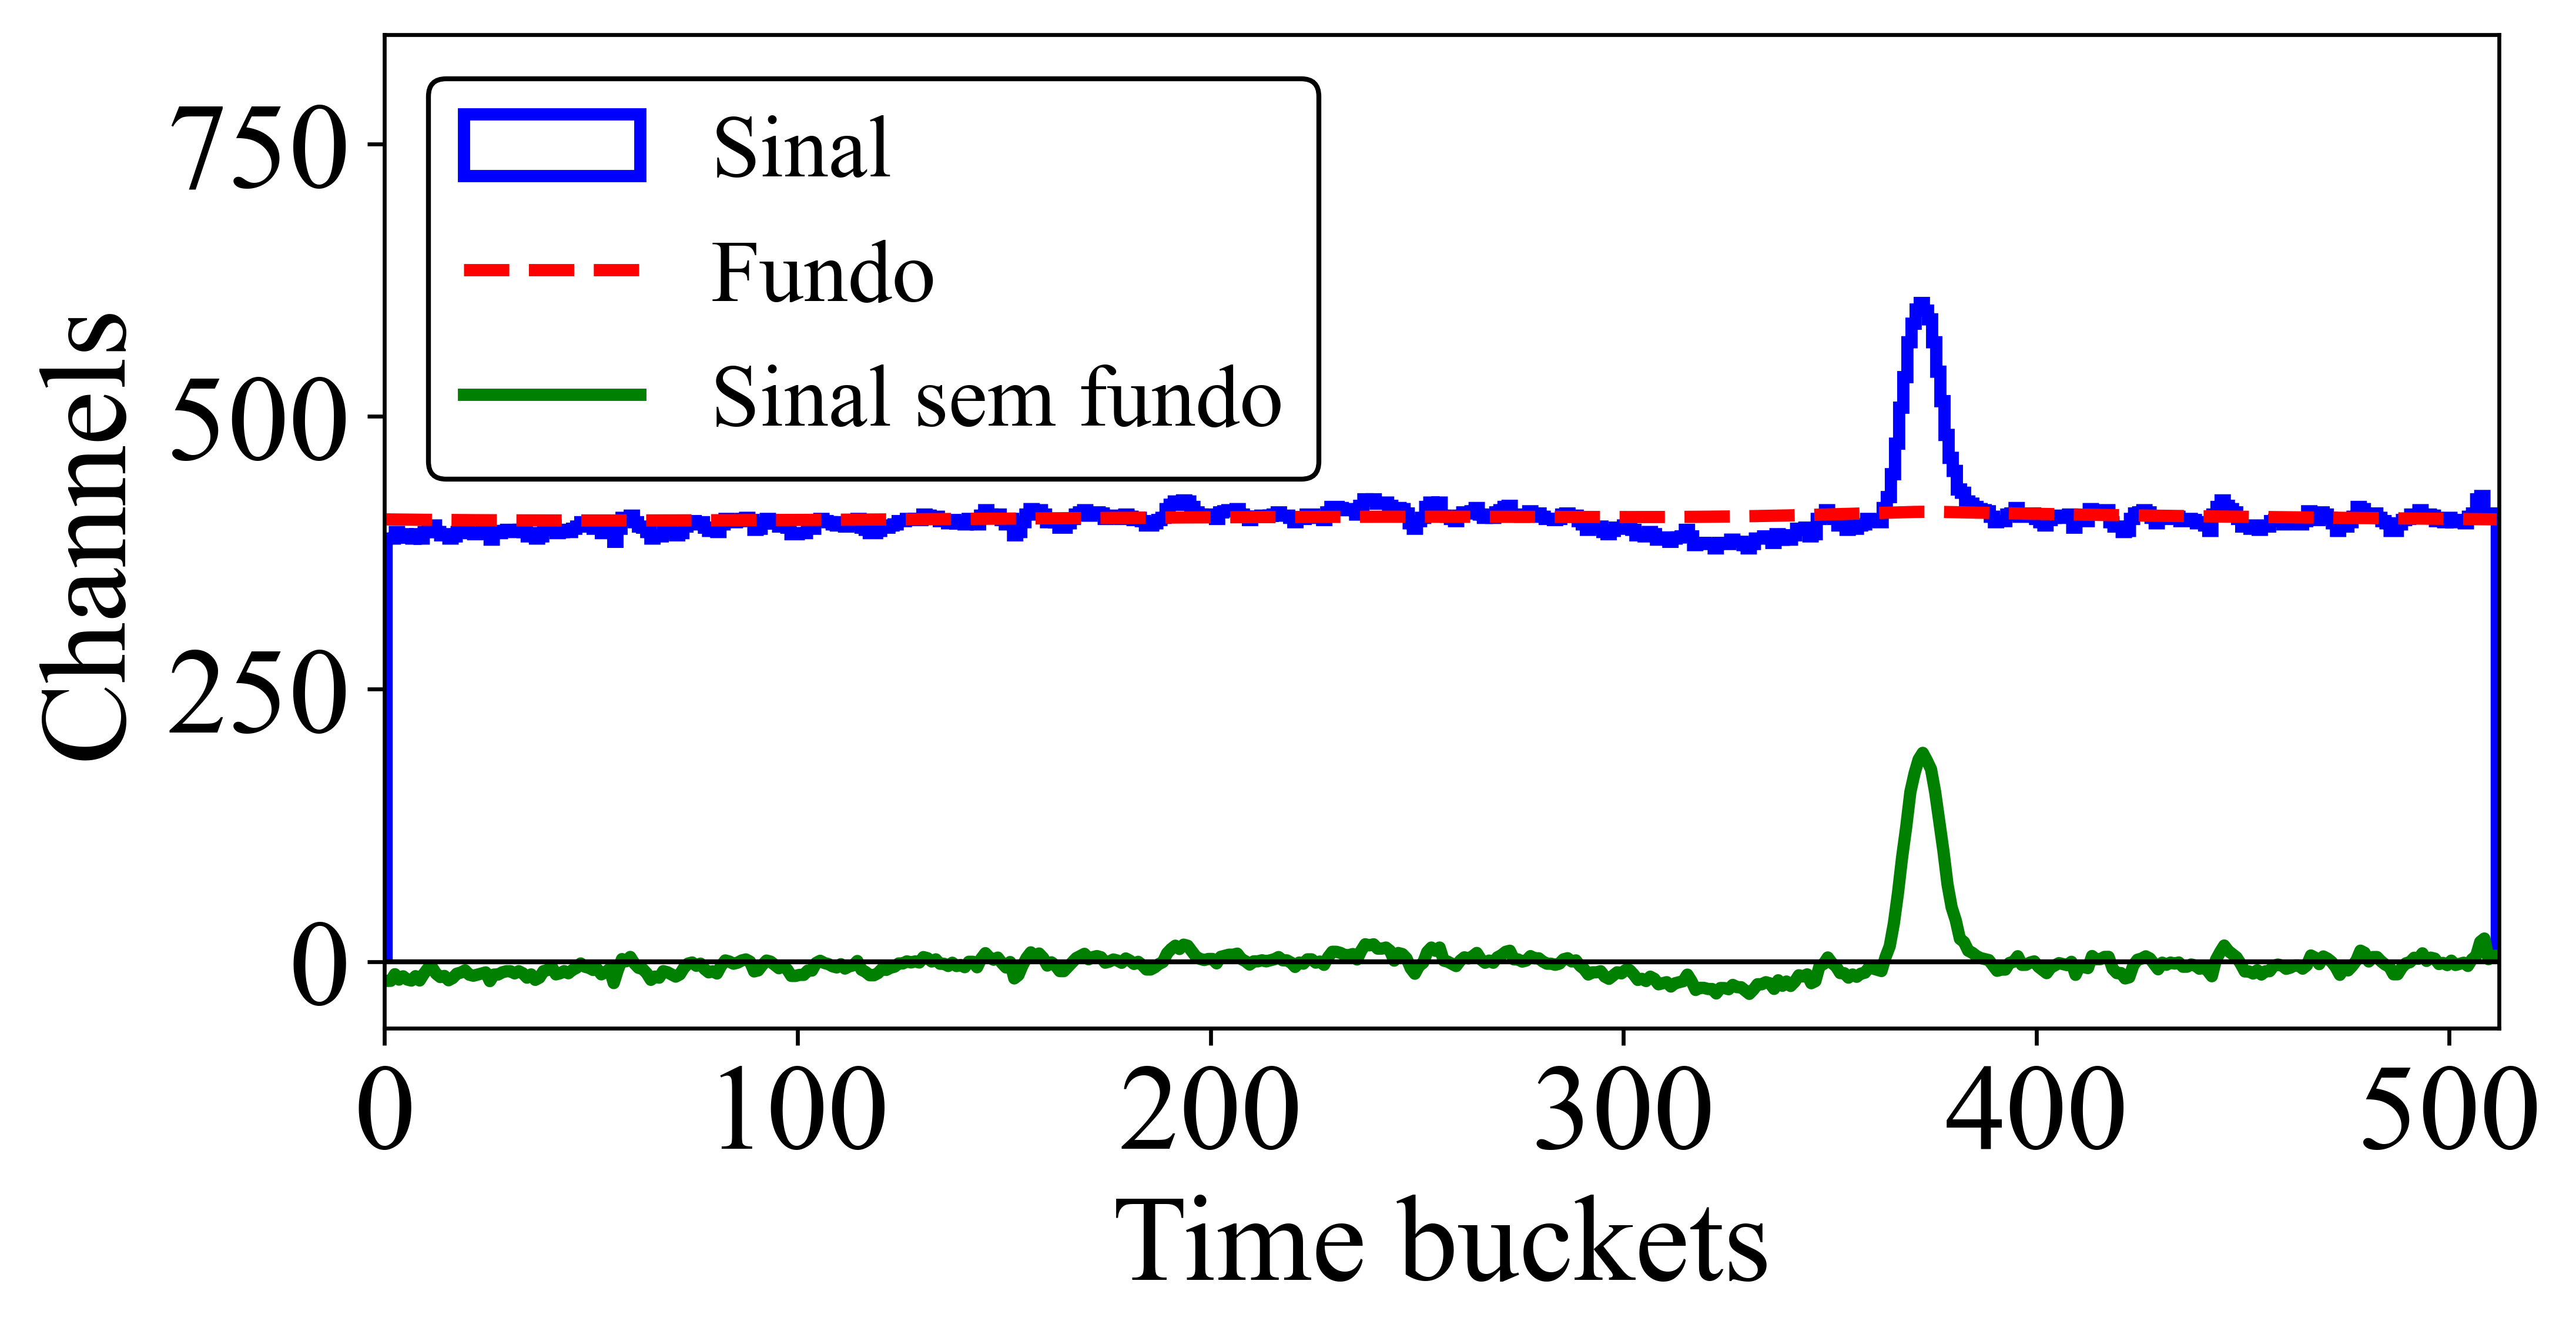
\includegraphics[scale=0.42]{figs/bs_fourier_1.png}
        \caption{}
        \label{subfig:bs_fourier_1}
    \end{subfigure}%
    \hfill
    \begin{subfigure}[c]{0.45\textwidth}
        % \centering
        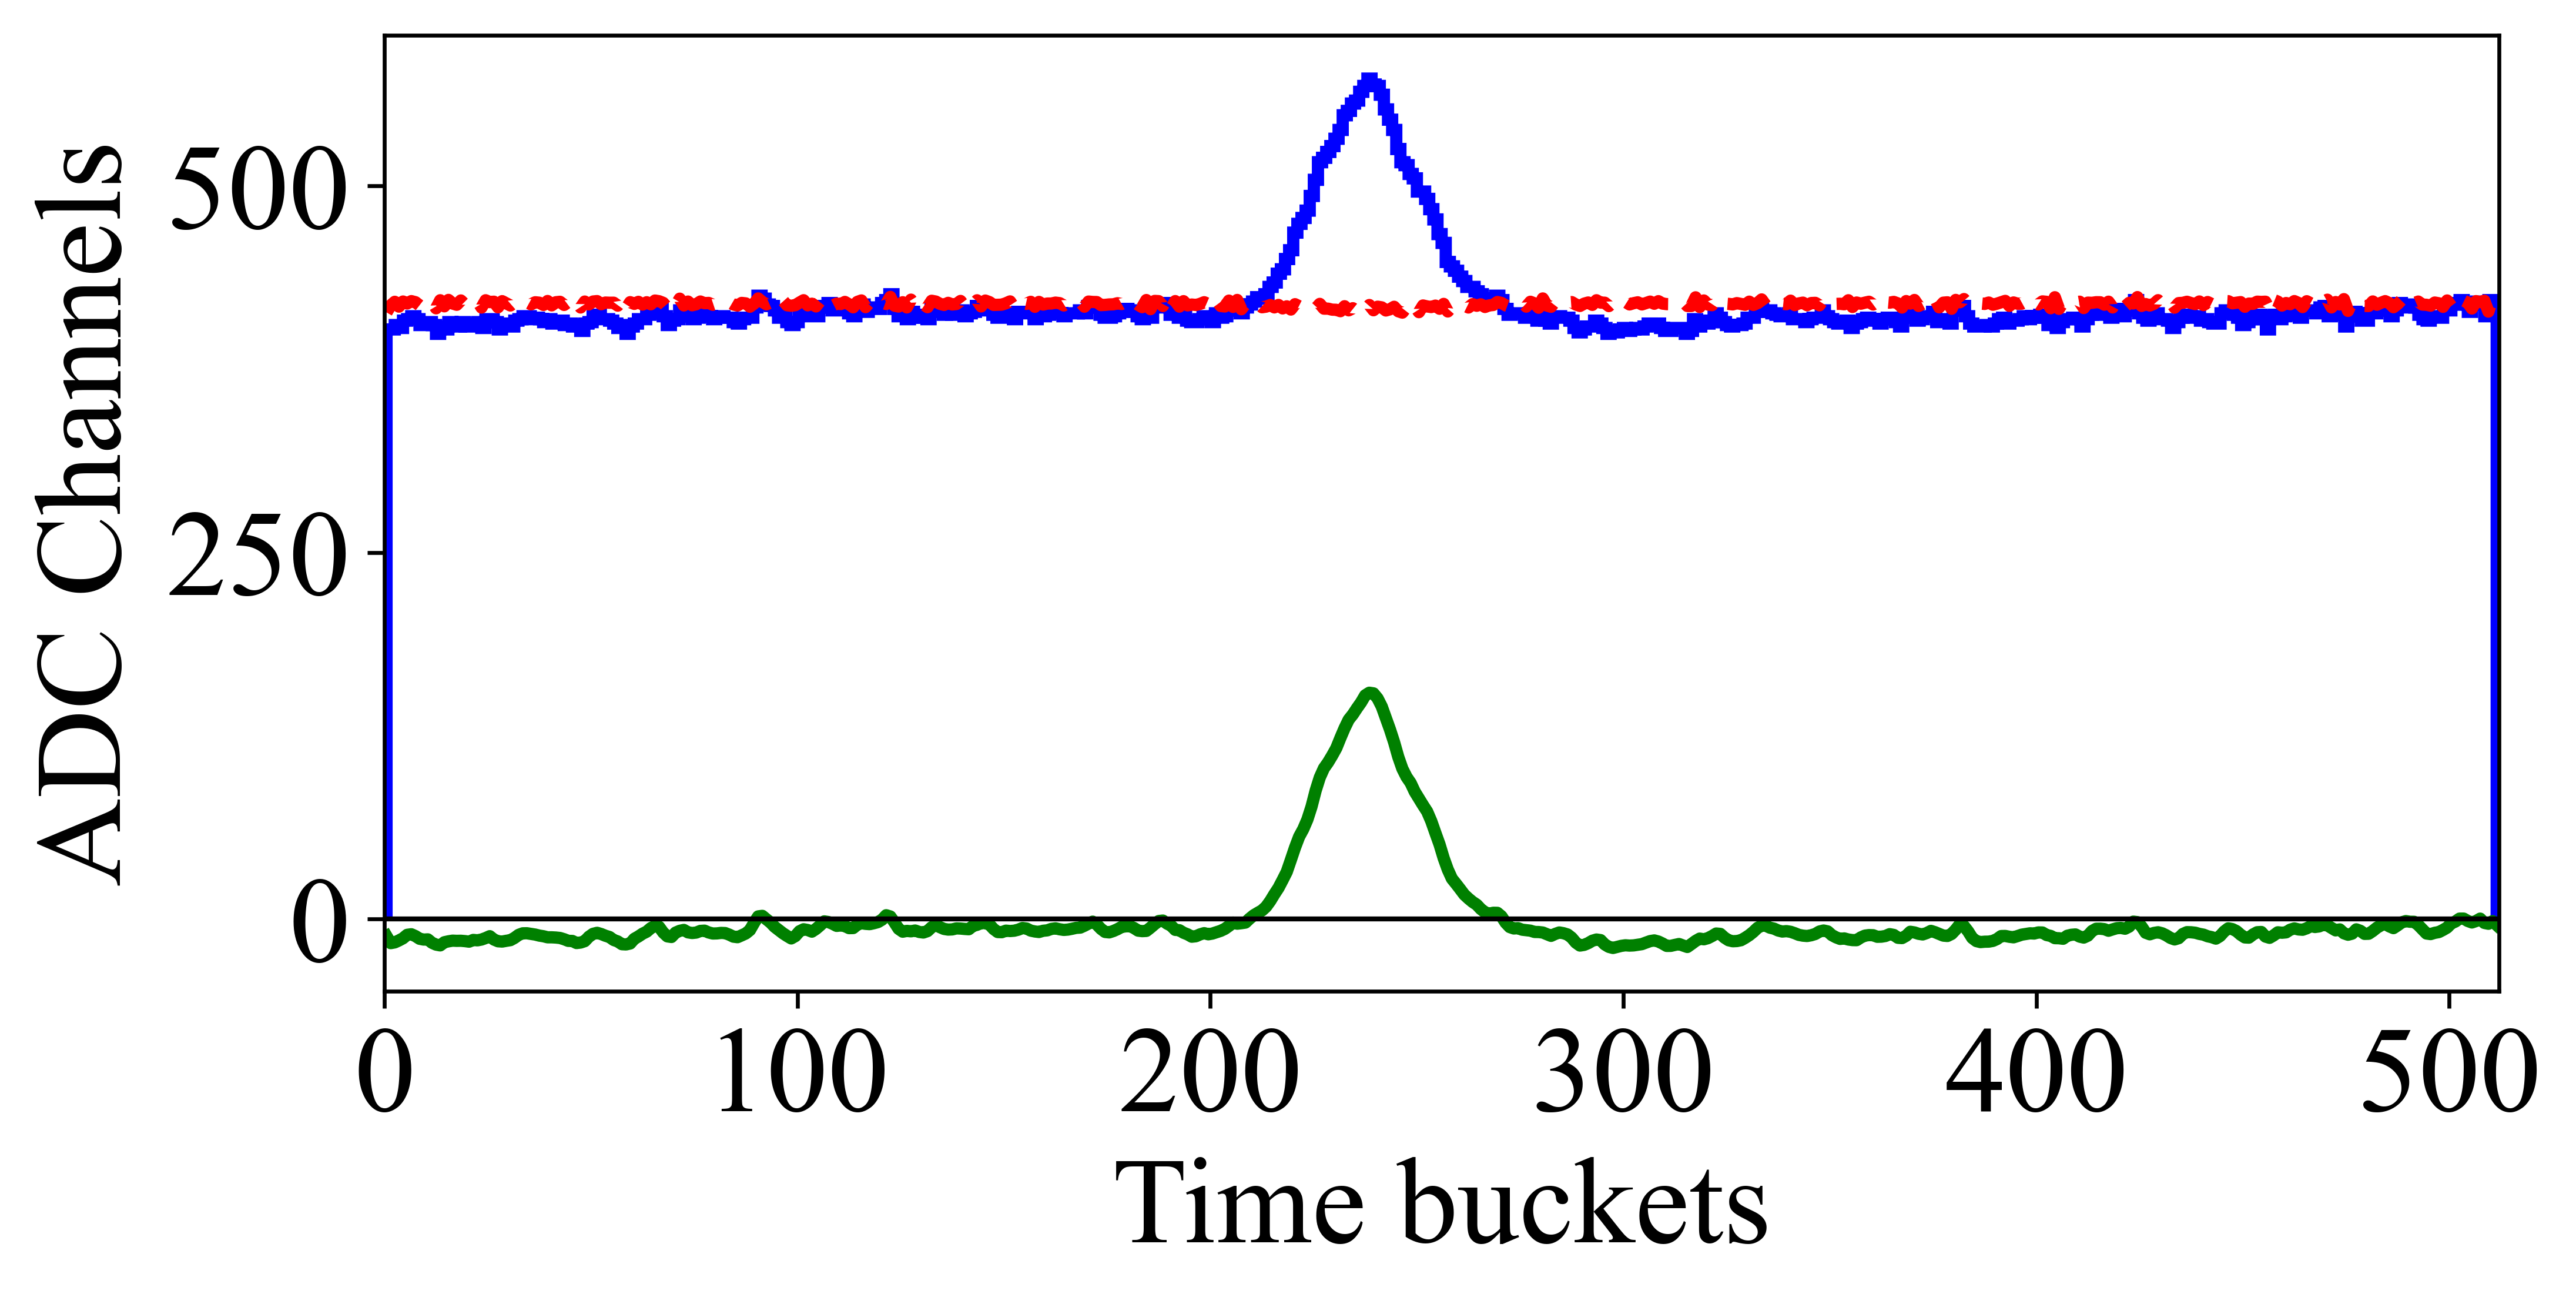
\includegraphics[scale=0.42]{figs/bs_fourier_2.png}
        \caption{}
        \label{subfig:bs_fourier_2}
    \end{subfigure}
    \begin{subfigure}[b]{0.45\textwidth}
        \centering
        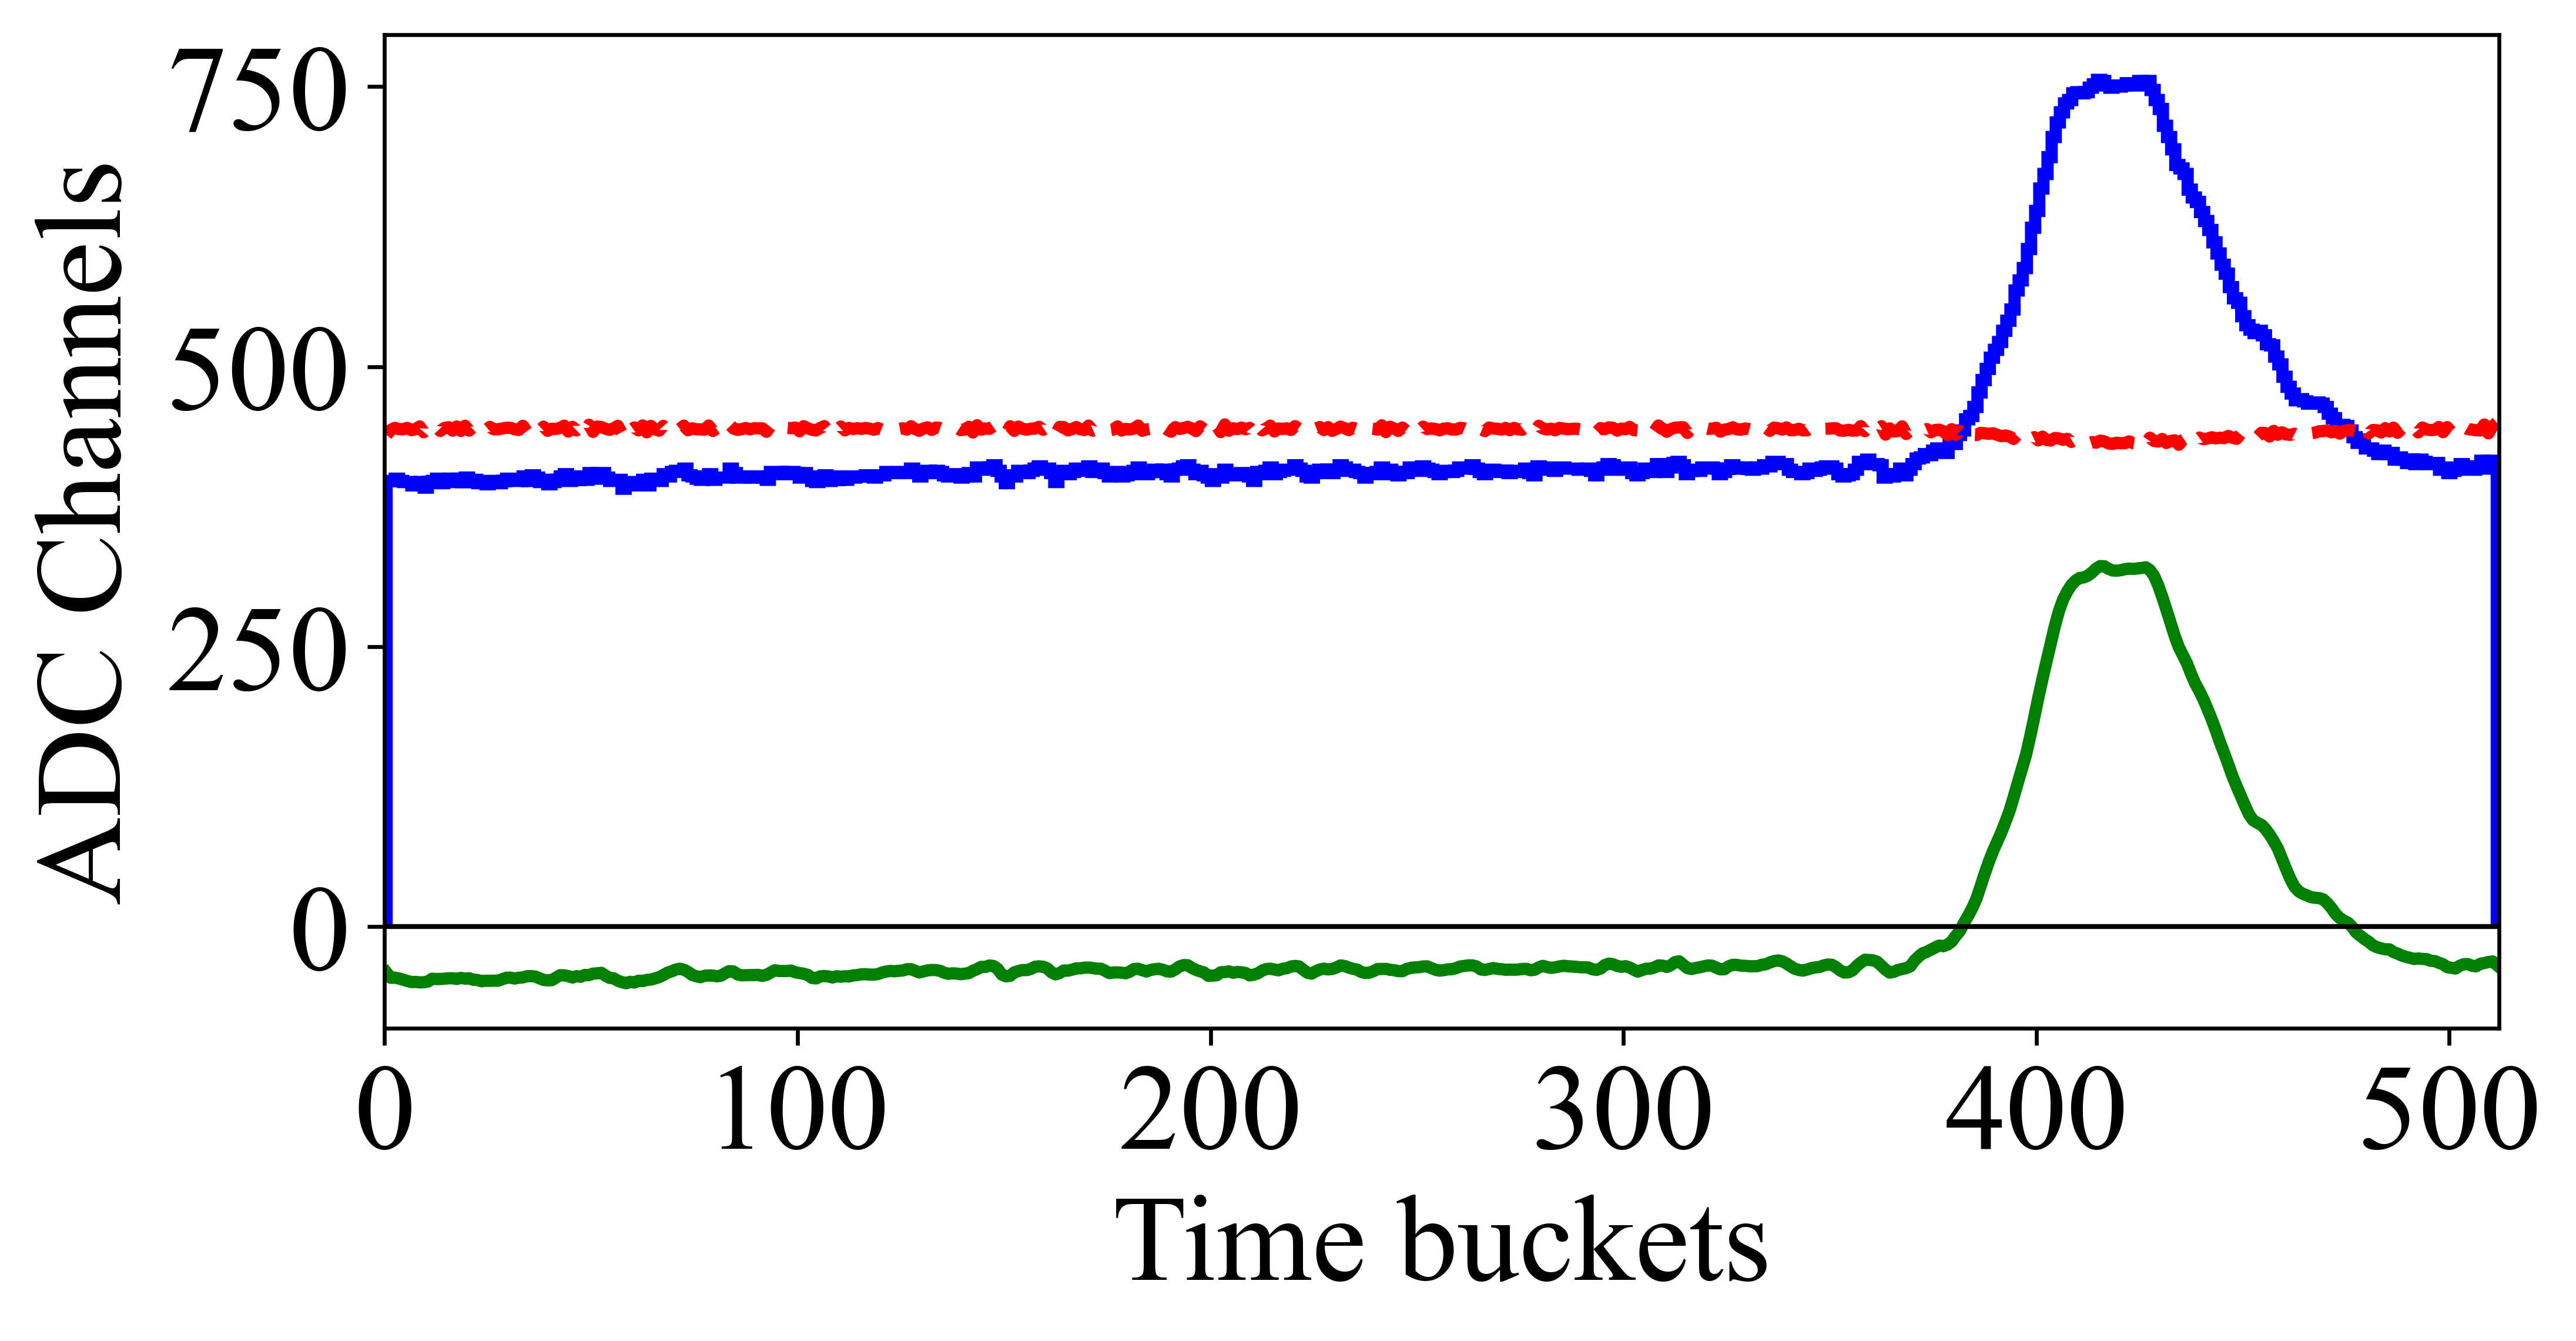
\includegraphics[scale=0.42]{figs/bs_fourier_3.png}
        \caption{}
        \label{subfig:bs_fourier_3}
    \end{subfigure}%
    \hfill
    \begin{subfigure}[b]{0.45\textwidth}
        \centering
        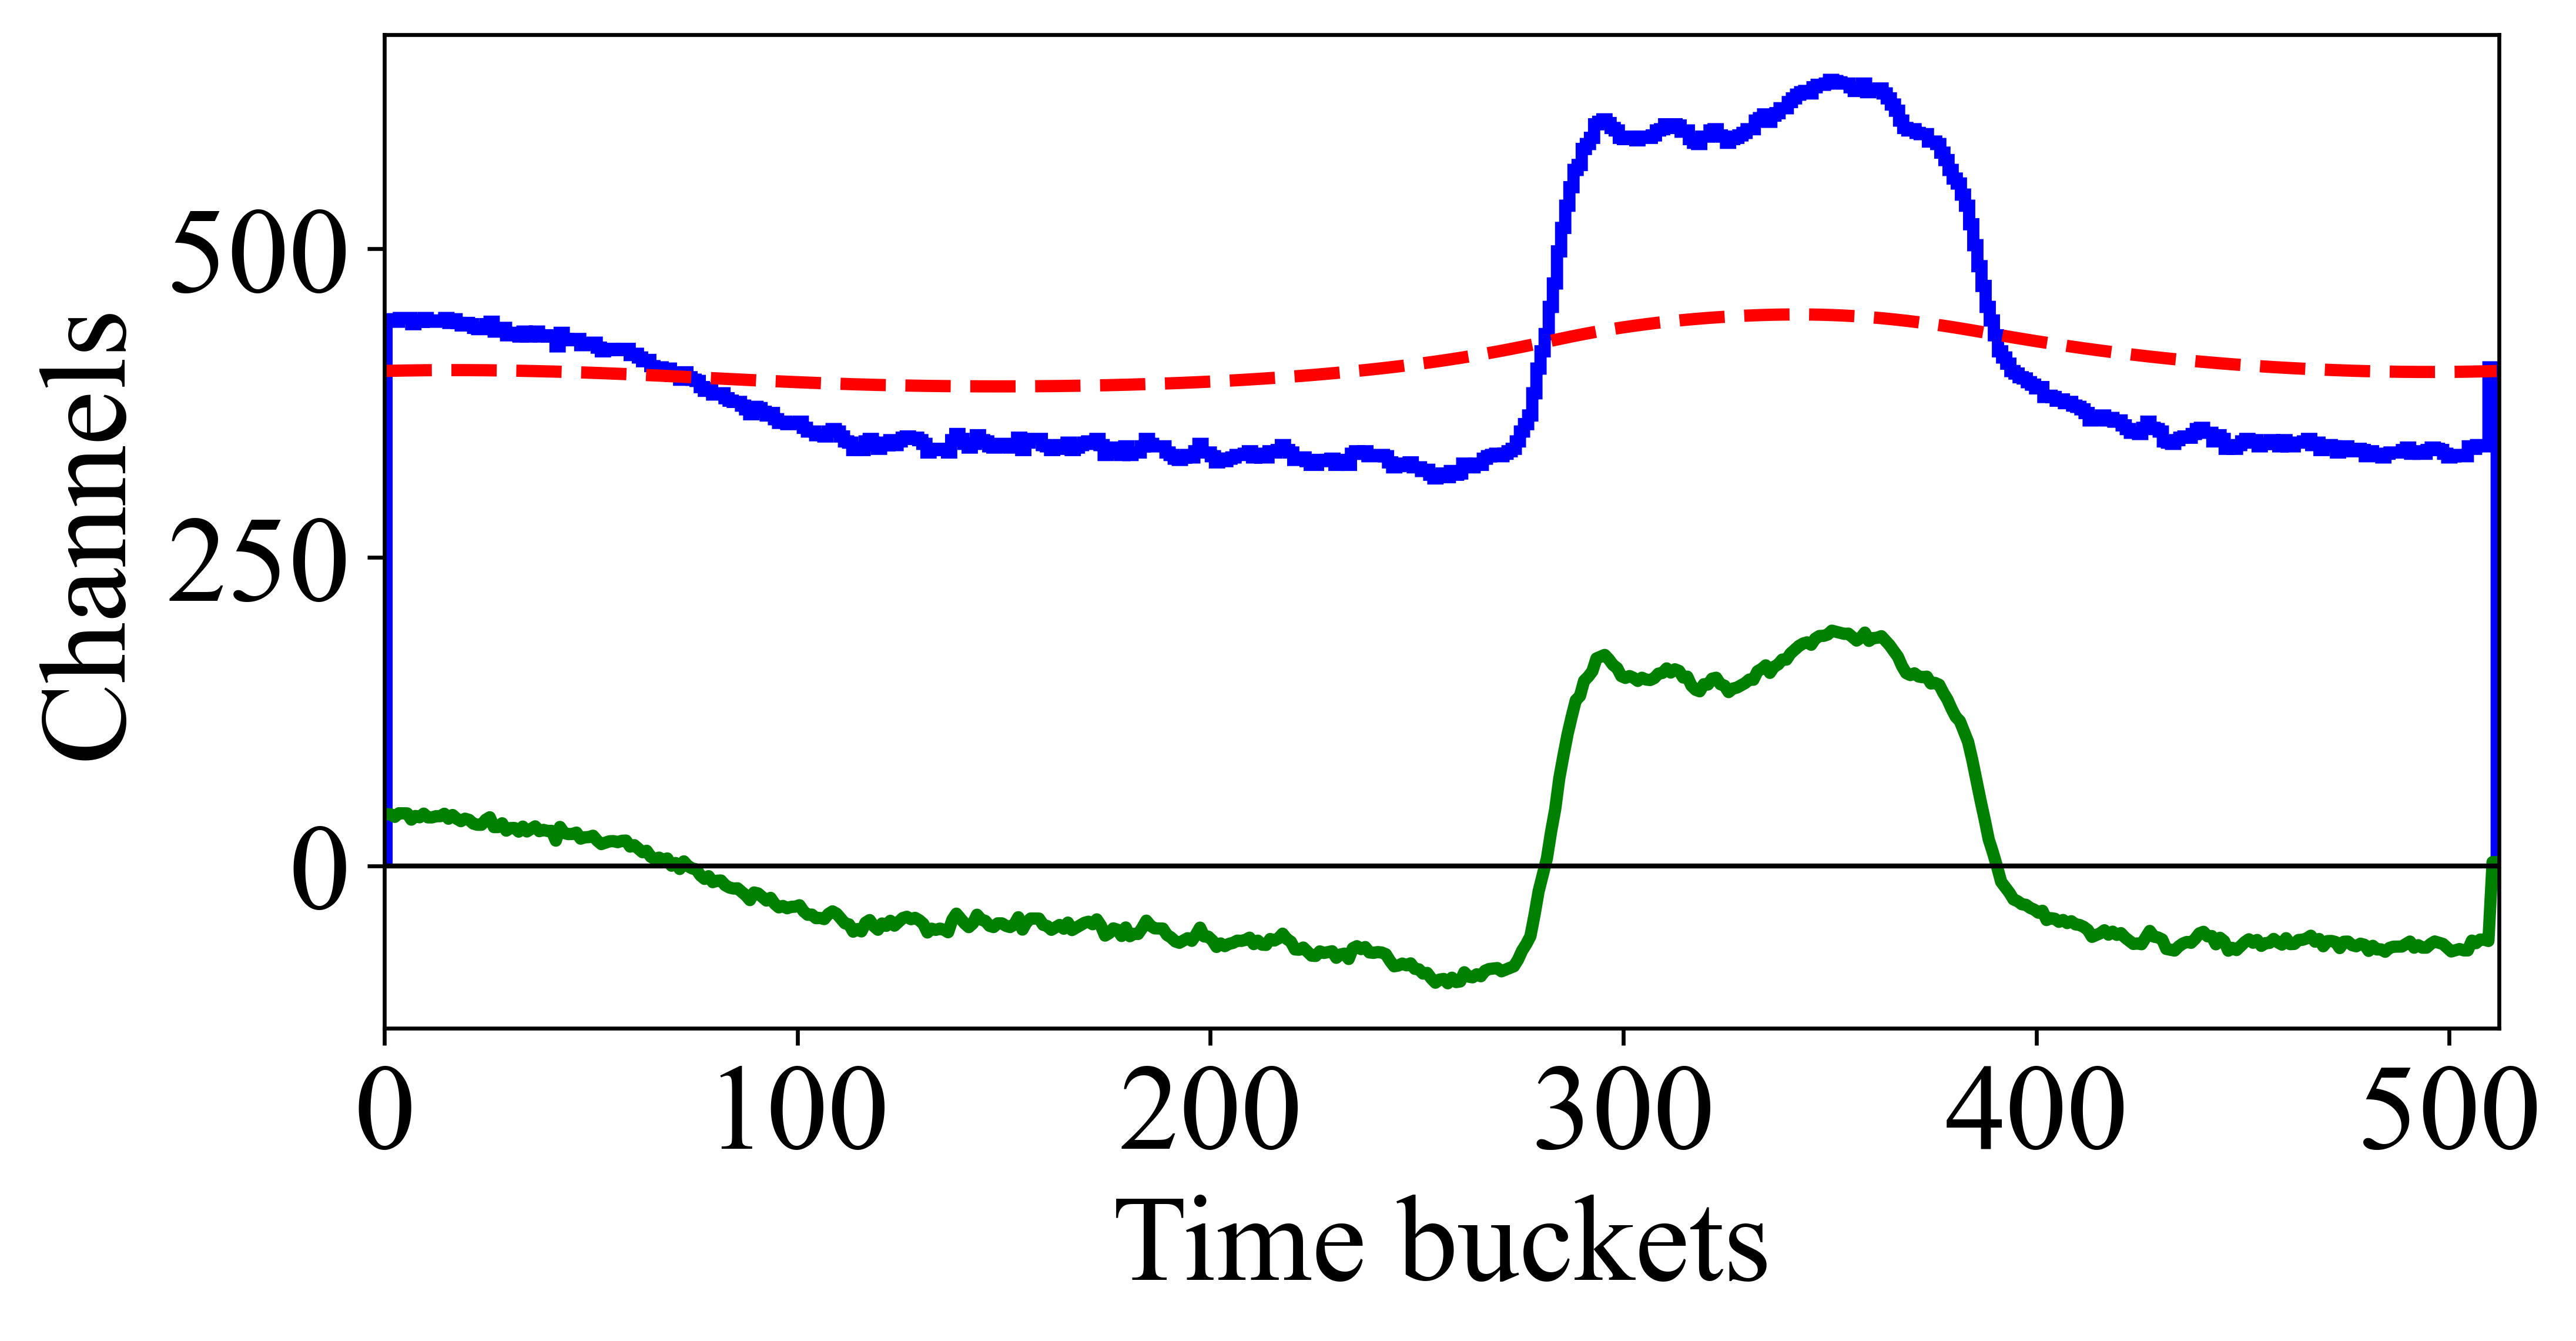
\includegraphics[scale=0.42]{figs/bs_fourier_4.png}
        \caption{}
        \label{subfig:bs_fourier_4}
    \end{subfigure}
\caption{Histogramas com as respectivas baselines (linhas tracejadas) estimadas pelo método da convolução. O espectro resultante (sem o fundo) está em verde.}
\label{fig:bs_fourier_exs}
\end{figure}

% Dos exemplo acima em muitos casos, acaba estimando o sinal original, na região do pulso, menor do que deveria ser, fazendo com que o sinal tenha menos carga do que deveria.

\par Fica claro que visualmente, por exemplo na figura \ref{subfig:bs_fourier_4}, que o filtro utilizado não é a melhor função resposta do detector. Poderia-se estimar essa função resposta empiricamente, porém os canais auxiliares chamados de \textit{Fixed Pattern Noise} (FPN) \cite{GET} usados para esta estimativa não foram armazenados. Portanto, a estimativa do fundo foi feita sinal por sinal \cite{FORTINO2022166497, GET}. Para isso, o fundo foi determinado usando o algoritmo \textsc{background removal} da biblioteca TSpectrum do ROOT \cite{root}. A função tem a capacidade de separar o fundo dos picos presentes no espectro \cite{BKG_1, BKG_2, BKG_3}. Exemplos de estimativa do fundo estão na figura \ref{fig:ex_sinal_bkg}.

%, pois o fundo é não analítico\cite{GET}. Para um resultado mais adequado, o fundo será determinado usando o algoritmo \textit{background removal} da biblioteca \textit{TSpectrum} do \textit{ROOT} \cite{root}. A função tem a capacidade de separar o fundo dos picos presentes no espectro\cite{BKG_1, BKG_2, BKG_3}. Exemplos de estimativa do fundo estão na figura \ref{fig:ex_sinal_bkg}.

\begin{figure}[H]
\centering
    \begin{subfigure}[b]{0.48\textwidth}
        \centering
        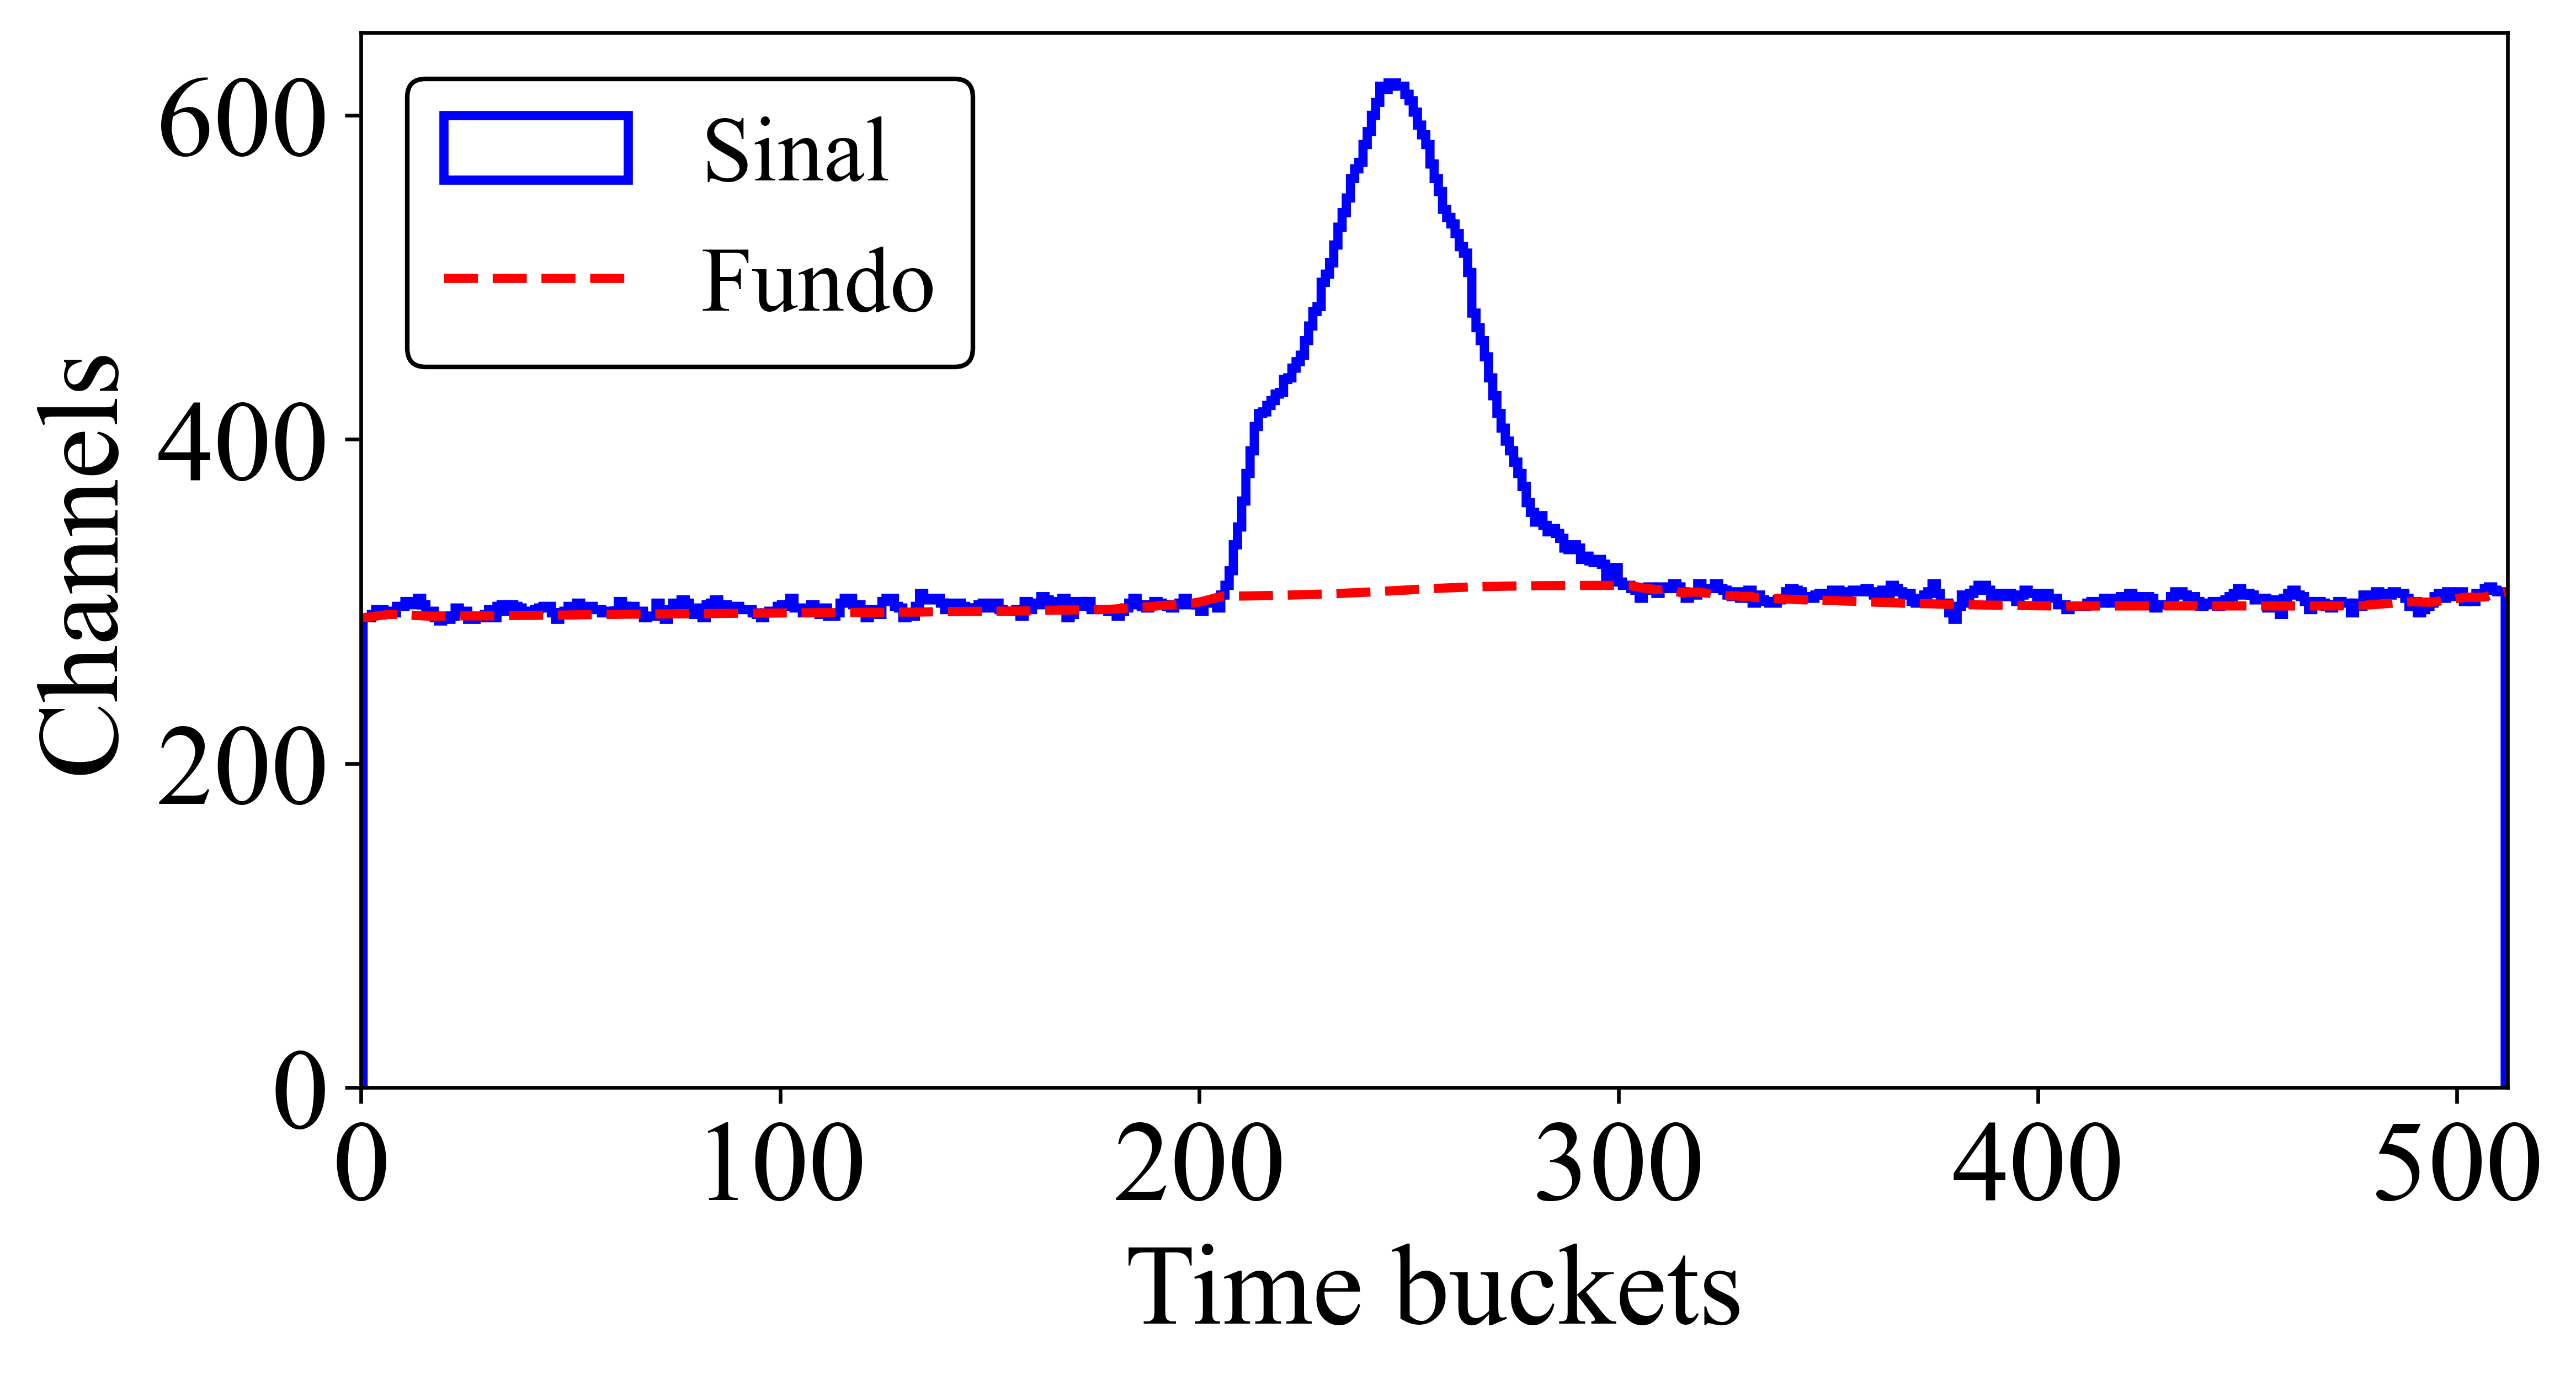
\includegraphics[scale=0.394]{figs/ex_sinal_bkg_1.png}
        \caption{}
        \label{subfig:ex_sinal_bkg_1}
    \end{subfigure}%
    \hfill
    \begin{subfigure}[b]{0.48\textwidth}
        \centering
        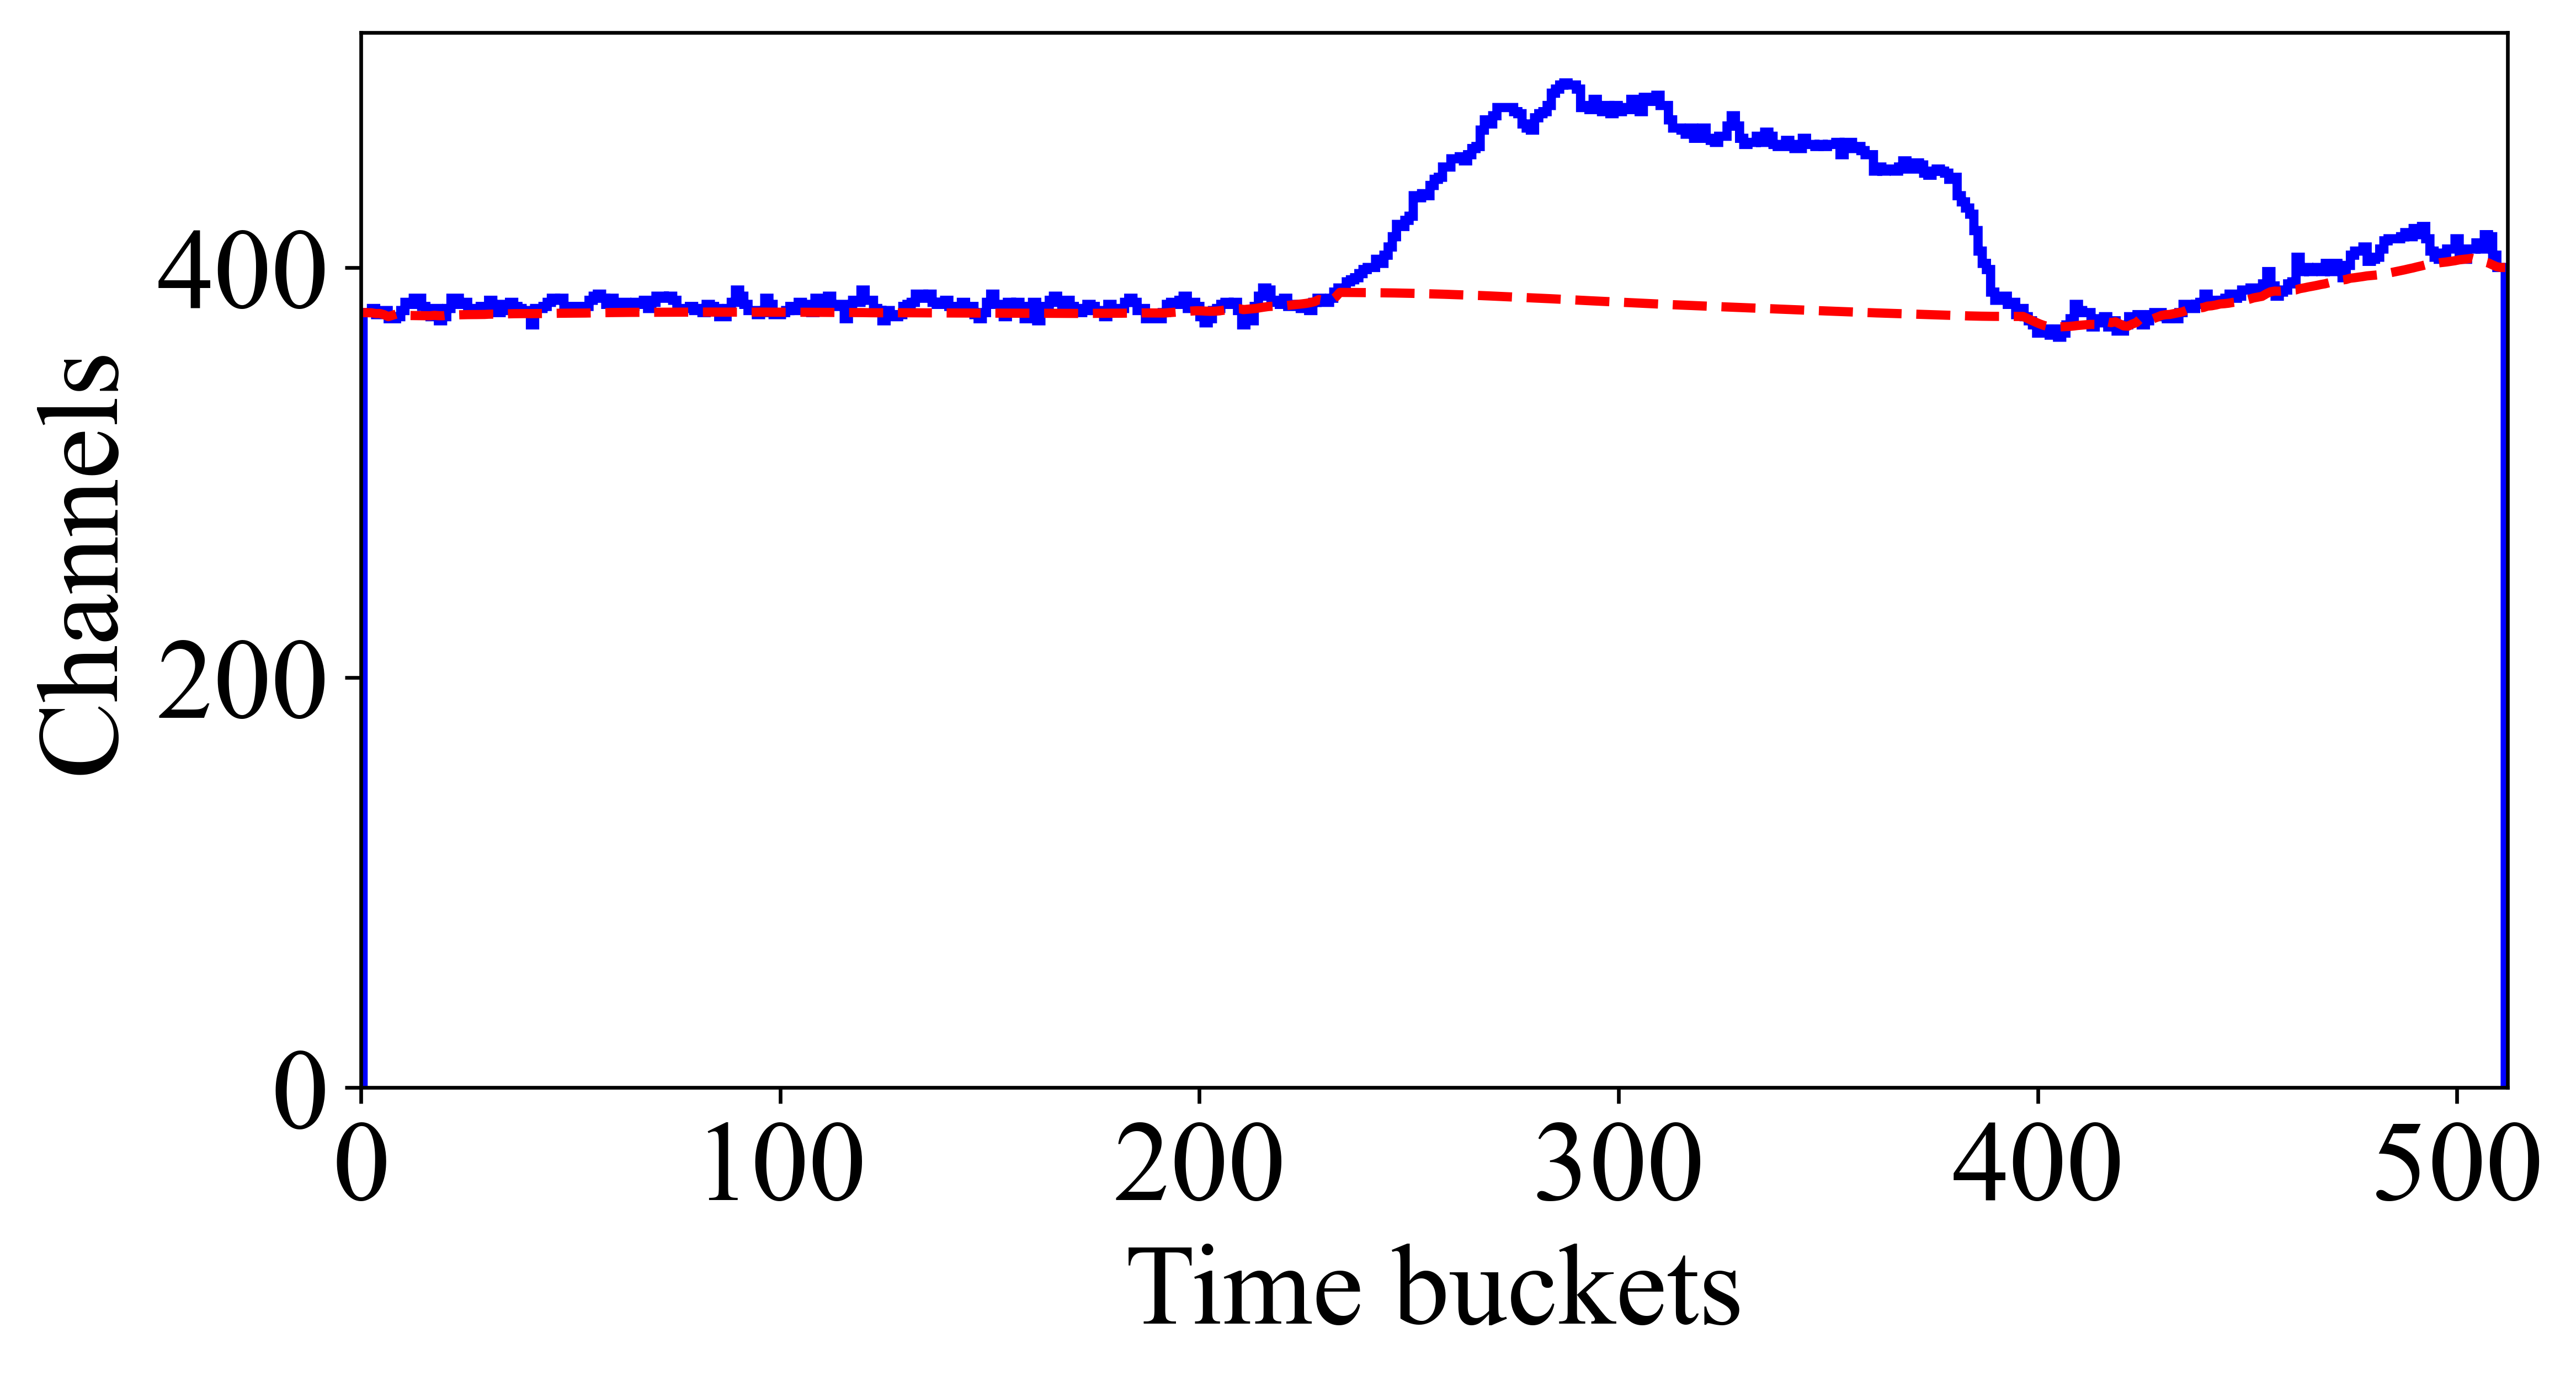
\includegraphics[scale=0.394]{figs/ex_sinal_bkg_2.png}
        \caption{}
        \label{subfig:ex_sinal_bkg_2}
    \end{subfigure}
    \begin{subfigure}[b]{0.48\textwidth}
        \centering
        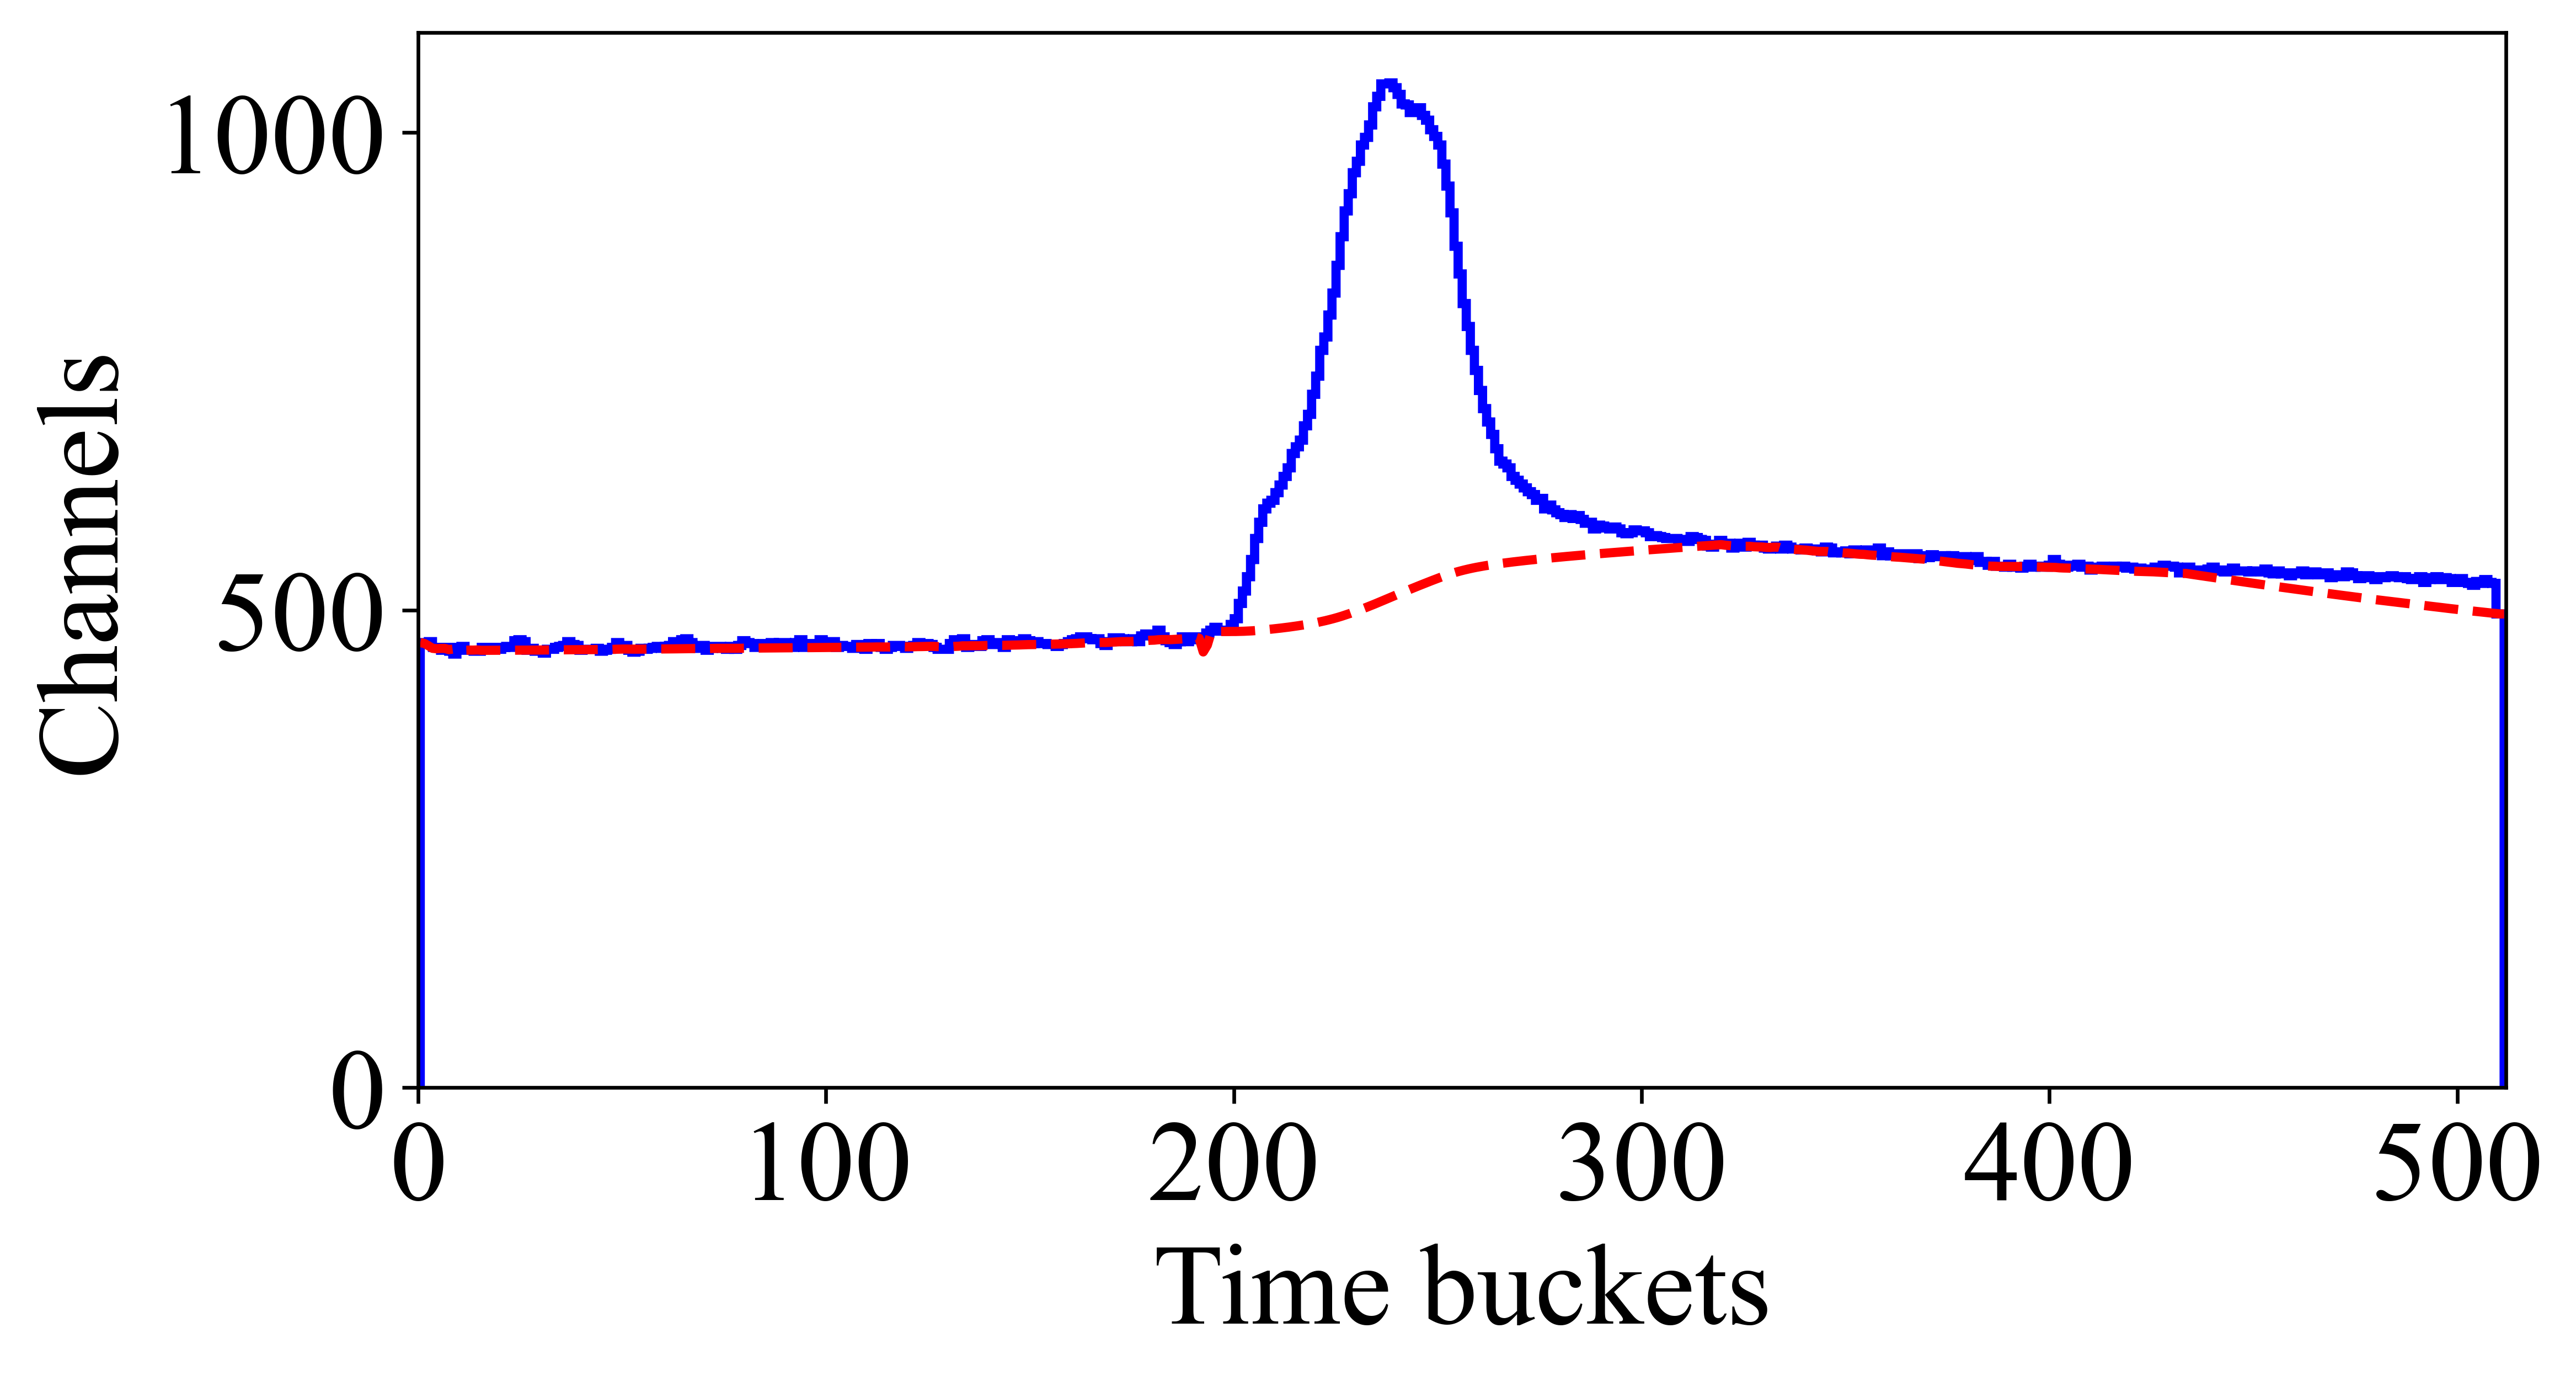
\includegraphics[scale=0.394]{figs/ex_sinal_bkg_3.png}
        \caption{}
        \label{subfig:ex_sinal_bkg_3}
    \end{subfigure}%
    \hfill
    \begin{subfigure}[b]{0.48\textwidth}
        \centering
        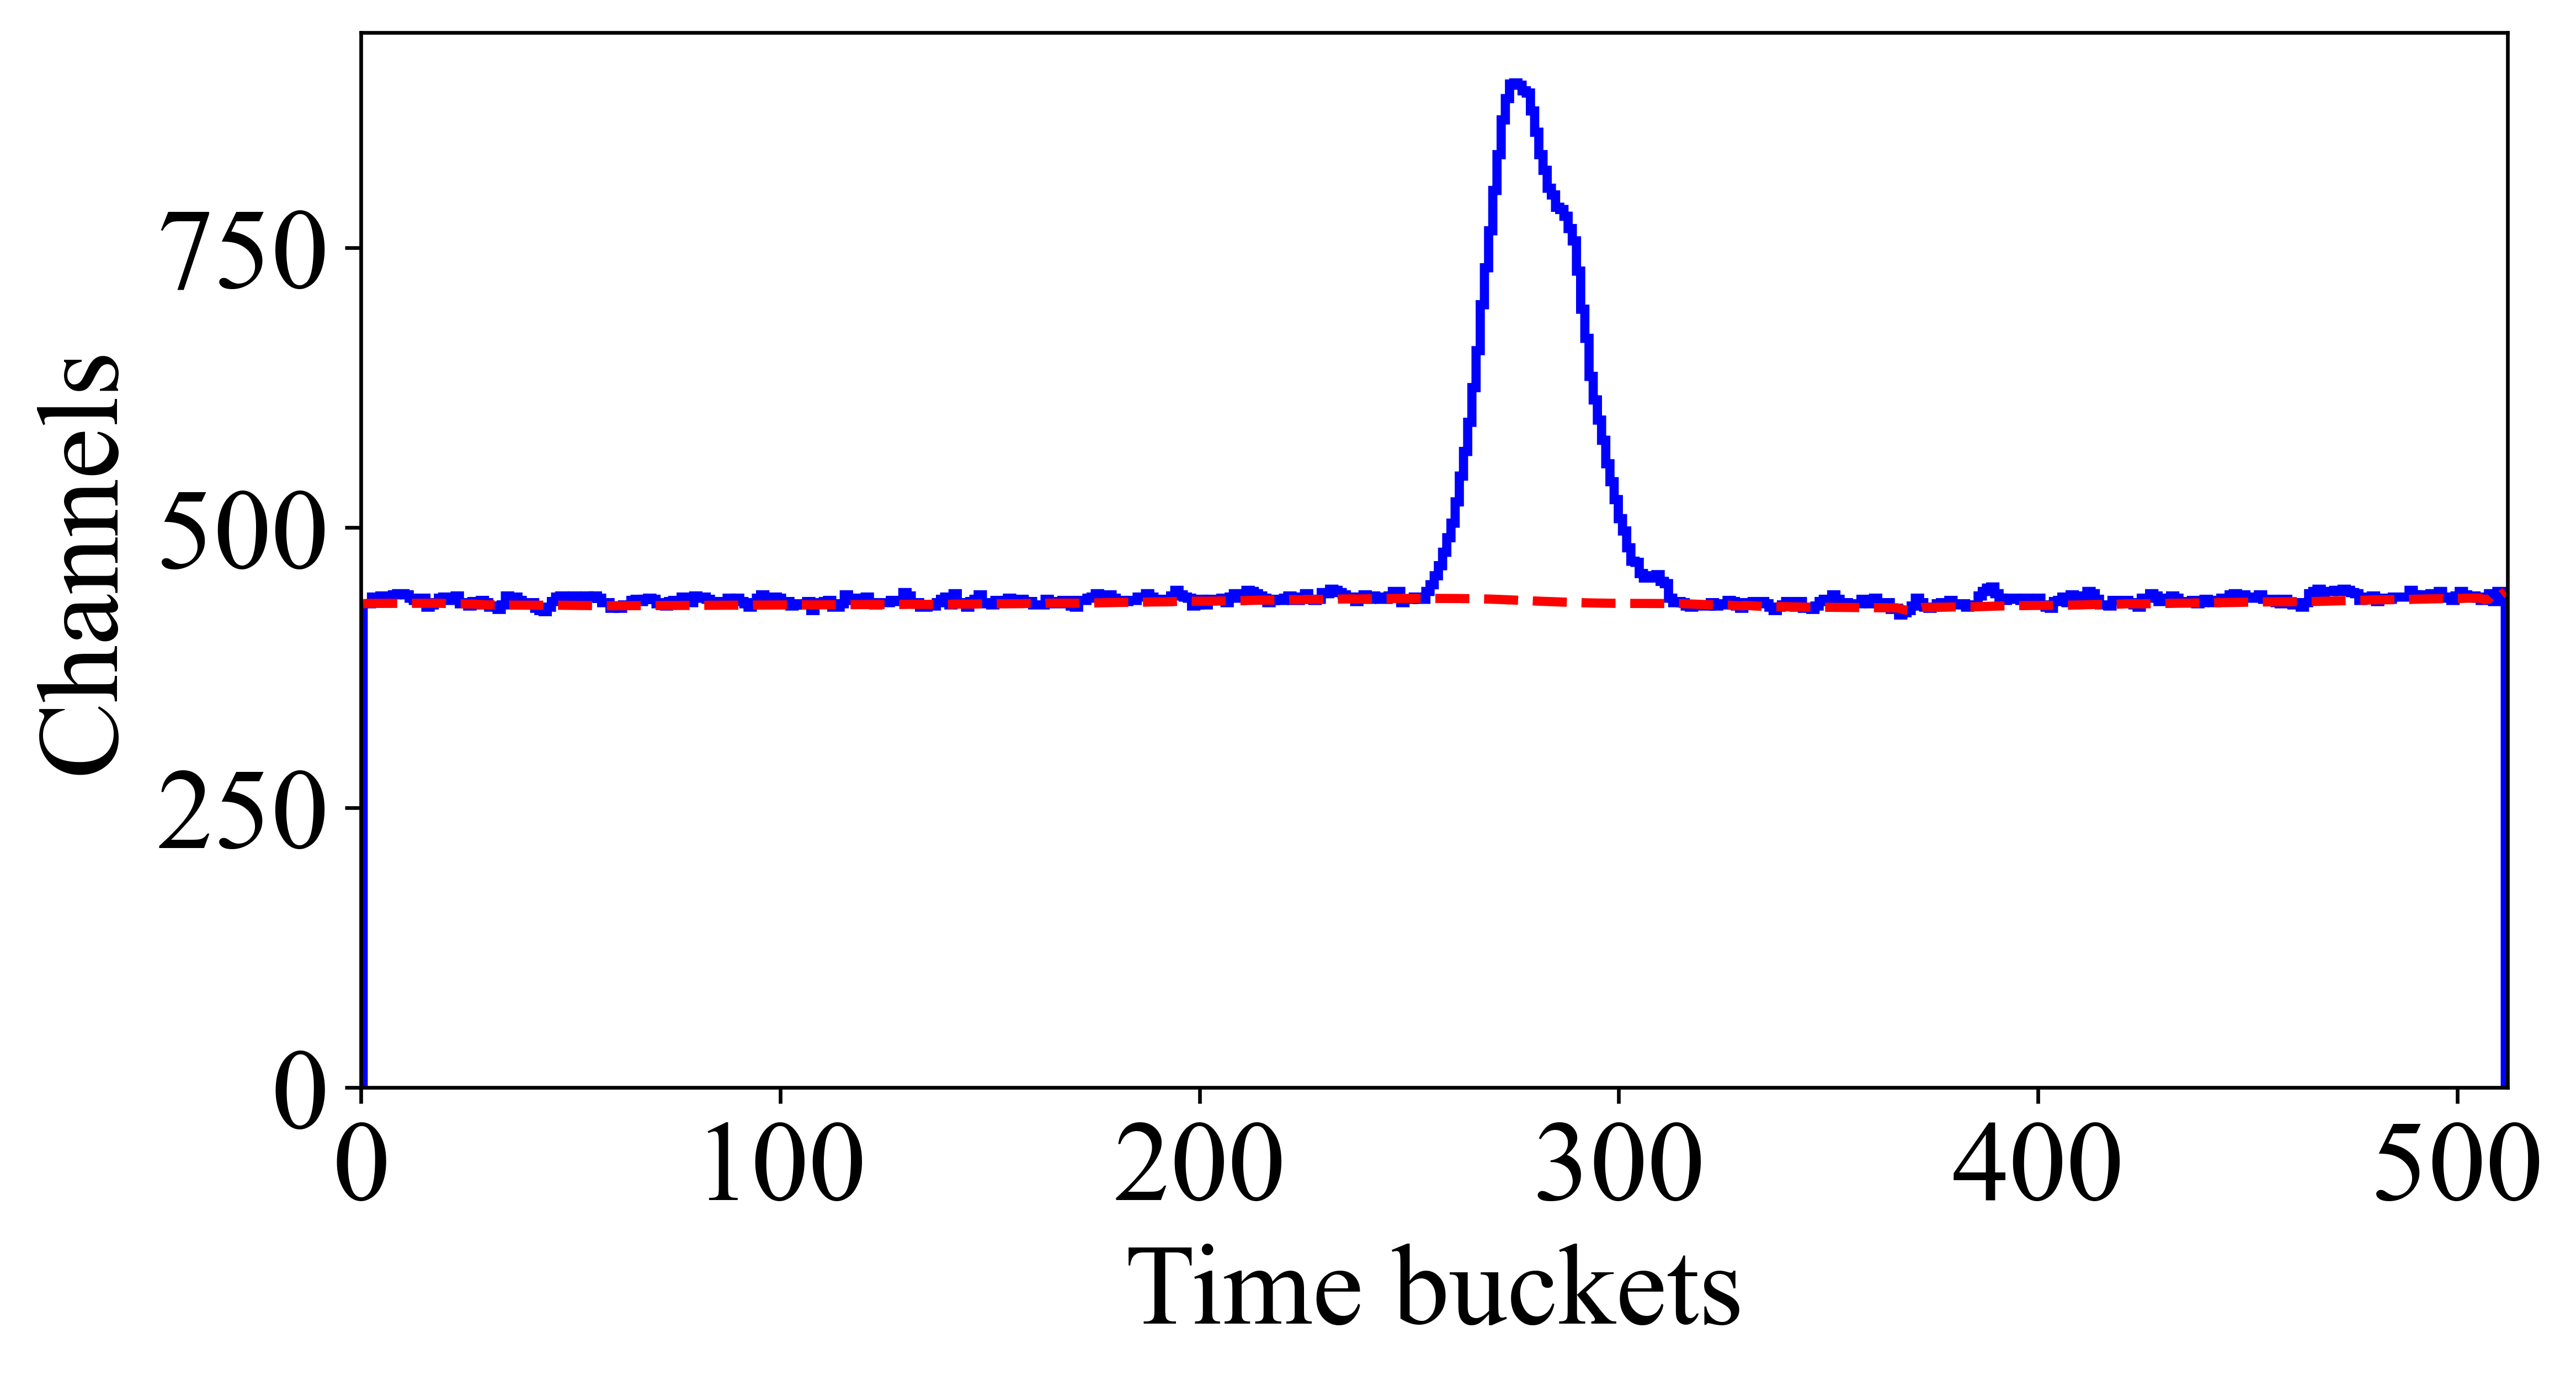
\includegraphics[scale=0.394]{figs/ex_sinal_bkg_4.png}
        \caption{}
        \label{subfig:ex_sinal_bkg_4}
    \end{subfigure}
\caption{Histogramas com as respectivas baselines (linhas tracejadas) calculadas pelo TSpectrum.}
\label{fig:ex_sinal_bkg}
\end{figure}

\par Os resultados dos cálculos para o ruído de fundo de cada sinal foram armazenados e usados na etapa seguinte de análise dos mesmos. Nessa próxima etapa a deconvolução dos sinais é realizada com os sinais tendo o ruído de fundo devidamente subtraído. Para diminuir as possíveis flutuações numéricas após a remoção do fundo, o valor mínimo do sinal sem o fundo deve ser zero. Uma vez eliminado o fundo, o código busca e identifica os picos e as correspondentes cargas do sinal. Como nem todos os sinais possuem pulsos únicos (não são uma composição de gaussianas), é necessário então realizar a deconvolução do sinal nas gaussianas que o compõe, conforme descrita na seção seguinte.

% Sem o fundo podemos buscar por todos os picos e suas cargas correspondentes no sinal. Não podemos identificar diretamente todos os picos pois muitos deles estão em sobreposição. Para isso foi feita a deconvolução do sinal, descrita na subseção \ref{subsec:pulses_deconv}.

% \par Com o fundo podemos então subtraí-lo do espectro. Podem aparecer valores negativos após a retirada do fundo, então para evitar esse problema o valor mínimo do sinal, após a retirada do fundo, é zero.


\subsection{Deconvolução do sinal}\label{subsec:pulses_deconv}

%\par Essa subseção descreve a etapa de deconvolução do sinal, que serve de banco de dados para o treinamento da rede neural descrita na subseção \ref{subsec:pulso_ml_deconv}.

\par Dependendo do ângulo da trajetória com respeito ao plano de detecção, a largura dos picos com cada pixel pode mudar (figura \ref{fig:get_signal}). Em termos gerais, os picos podem ser descritos como uma superposição de Gaussianas com uma largura fixa que é definida pelo eletrônica do alvo ativo. Precisamos então deconvoluir os picos em suas componentes. Para tanto utilizamos o algoritmo \textsc{gold deconvolution} presente na biblioteca TSpectrum do ROOT \cite{paper_gold_deconv}. O algoritmo tem como objetivo fazer a deconvolução do espectro, gerando uma função (nesse caso um pulso gaussiano) resposta de acordo com o desvio padrão dos pulsos. O sinal resposta corresponde ao espectro com as gaussianas não sobrepostas. Isso significa que foi necessário determinar qual o valor da largura dos pulsos para buscar a função resposta. A largura dos pulsos foi determinada fazendo a análise de sinais que possuem apenas 1 pico, fazendo um ajuste pelo método dos mínimos quadrados (MMQ) de uma gaussiana. Para buscar espectros com apenas um pico, foi usado o algoritmo de identificação de picos \textsc{peak\_finder}, presente na biblioteca do scipy \cite{scipy}, e para o ajuste da gaussiana foi usada o pacote \textsc{lmfit} \cite{lmfit}. O valor do desvio padrão encontrado foi de 4,09 (17) \textit{time buckets}. A largura escolhida foi ligeiramente maior pois, verificando empiricamente, em alguns casos o algoritmo separava o que deveria ser uma única gaussiana em duas. O valor do desvio padrão usado na deconvolução foi de 4,30 \textit{time buckets}. Foi determinado também o número de iterações do algoritmo de deconvolução. O número de iterações escolhido foi de 700, menos que isso o algoritmo não estava separando totalmente picos sobrepostos. O limiar para a escolha de um ponto como um pico foi definido como ter altura maior que 20\% do valor máximo do sinal. Resultados da deconvolução estão na figura \ref{fig:ex_sinal_deconv}.

\begin{figure}[H]
\centering
    \begin{subfigure}[b]{0.48\textwidth}
        \centering
        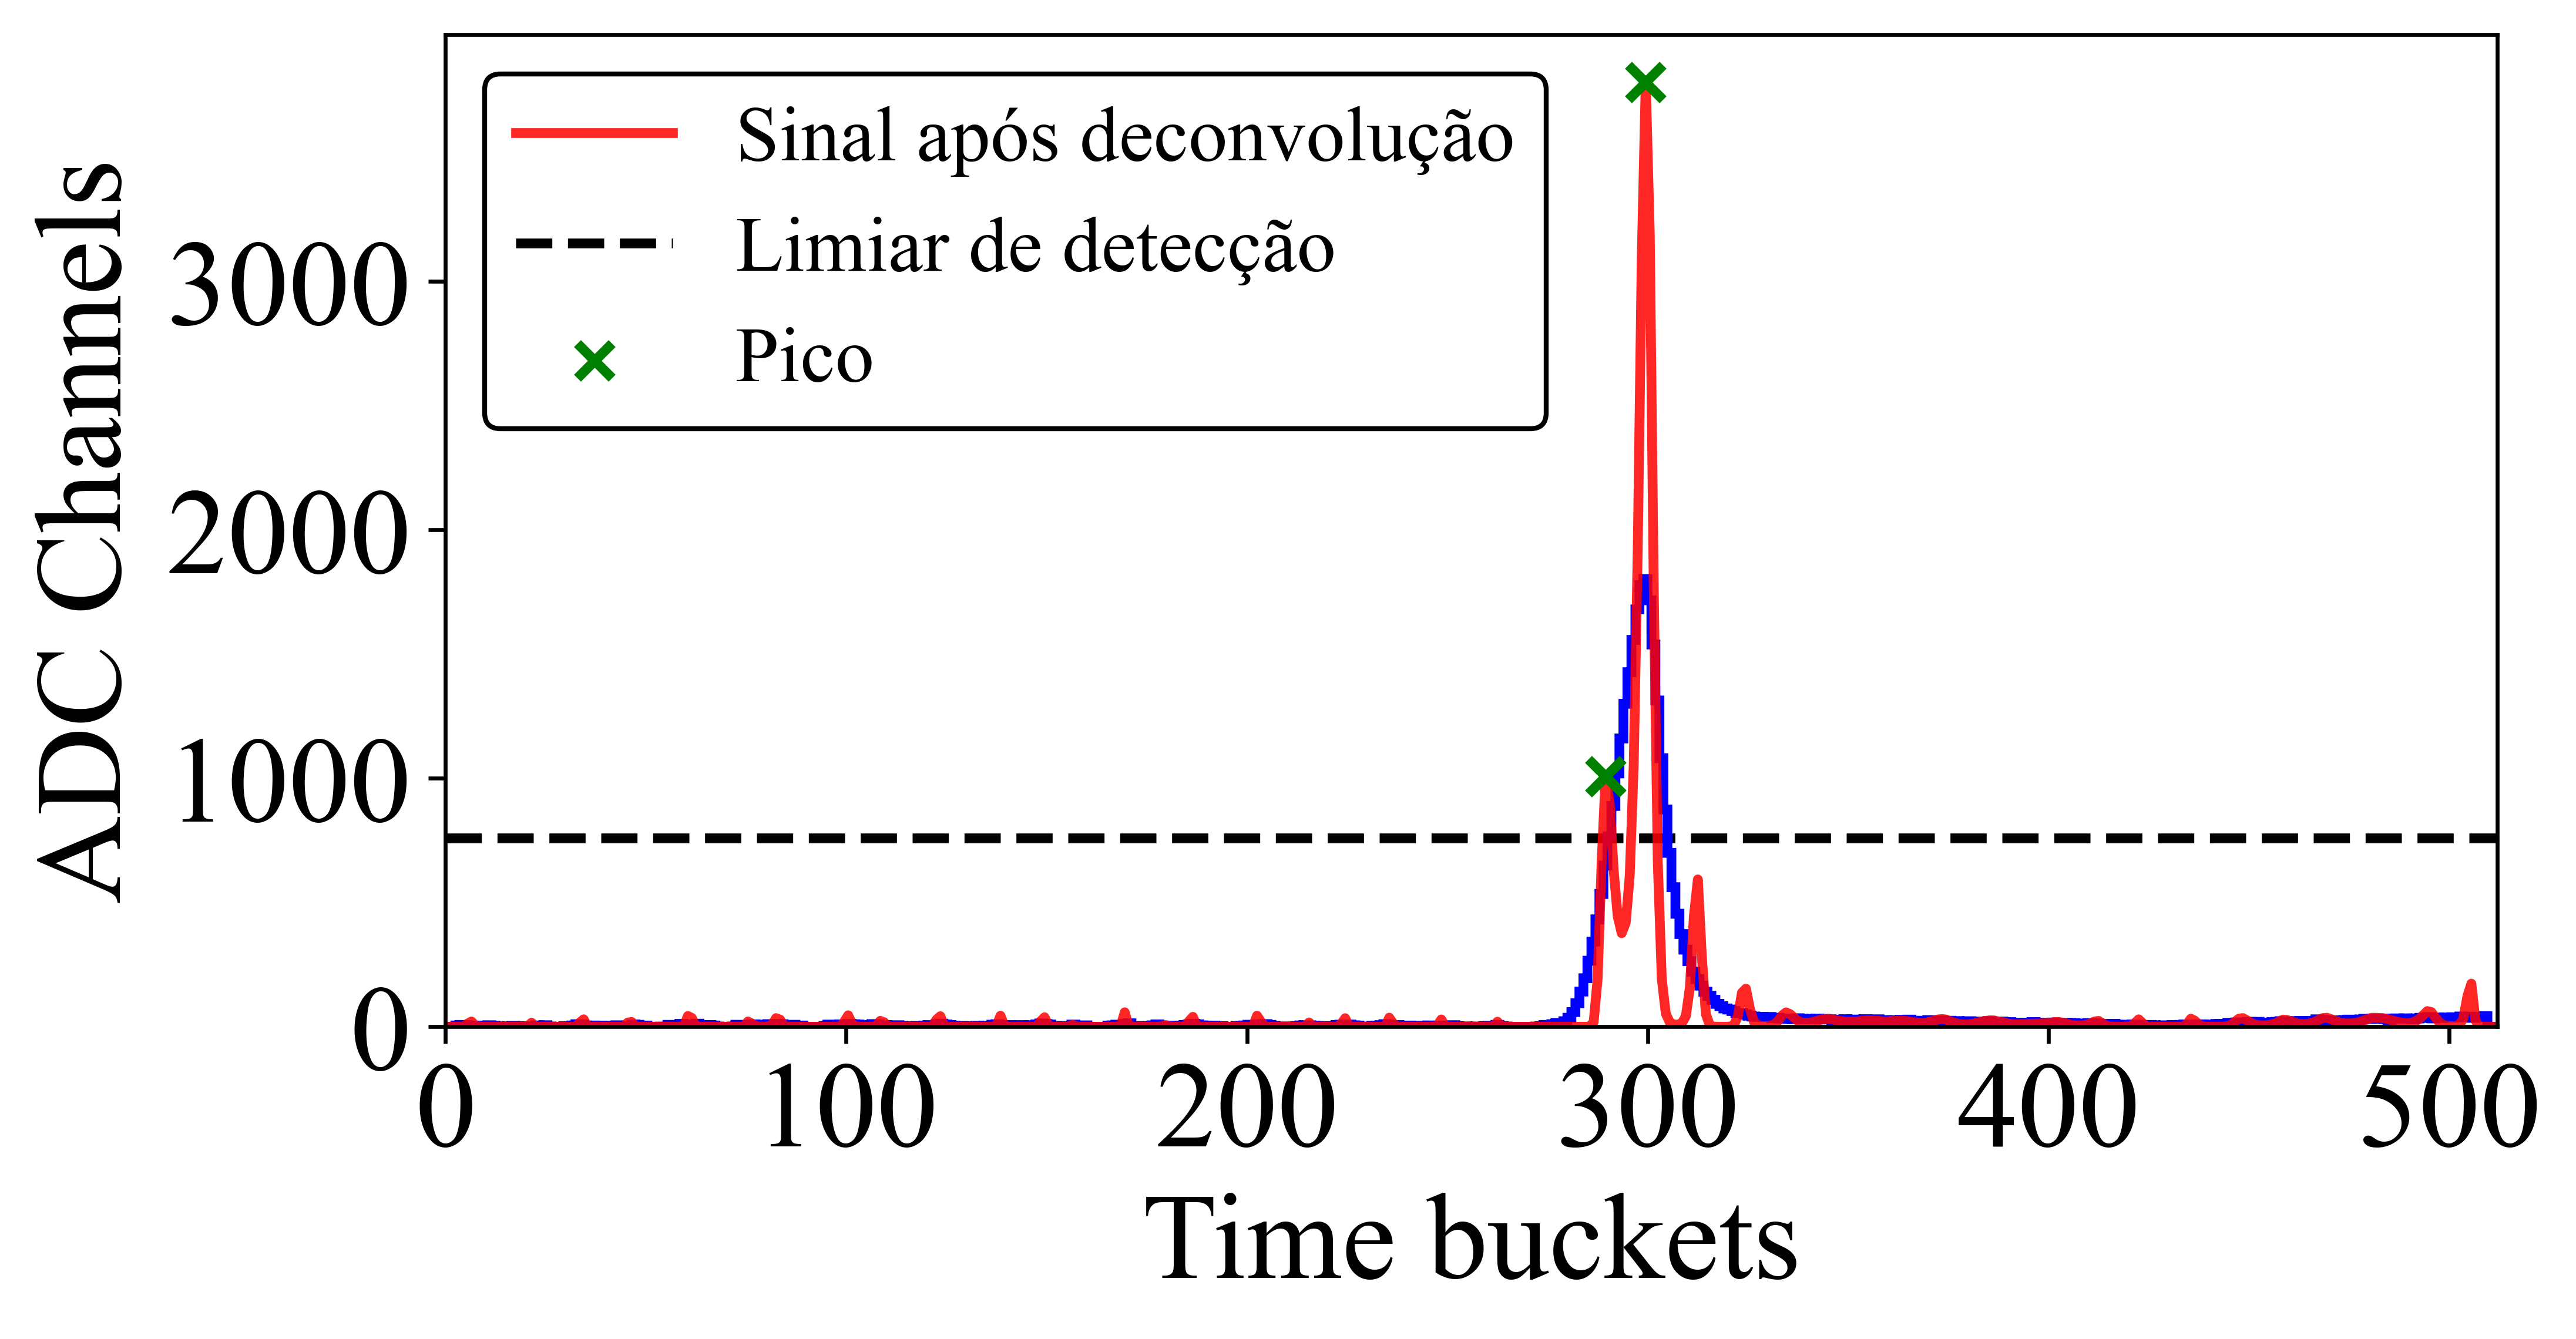
\includegraphics[scale=0.40]{figs/ex_deconv_1.png}
        \caption{}
        \label{subfig:ex_sinal_deconv_1}
    \end{subfigure}%
    \hfill
    \begin{subfigure}[b]{0.48\textwidth}
        \centering
        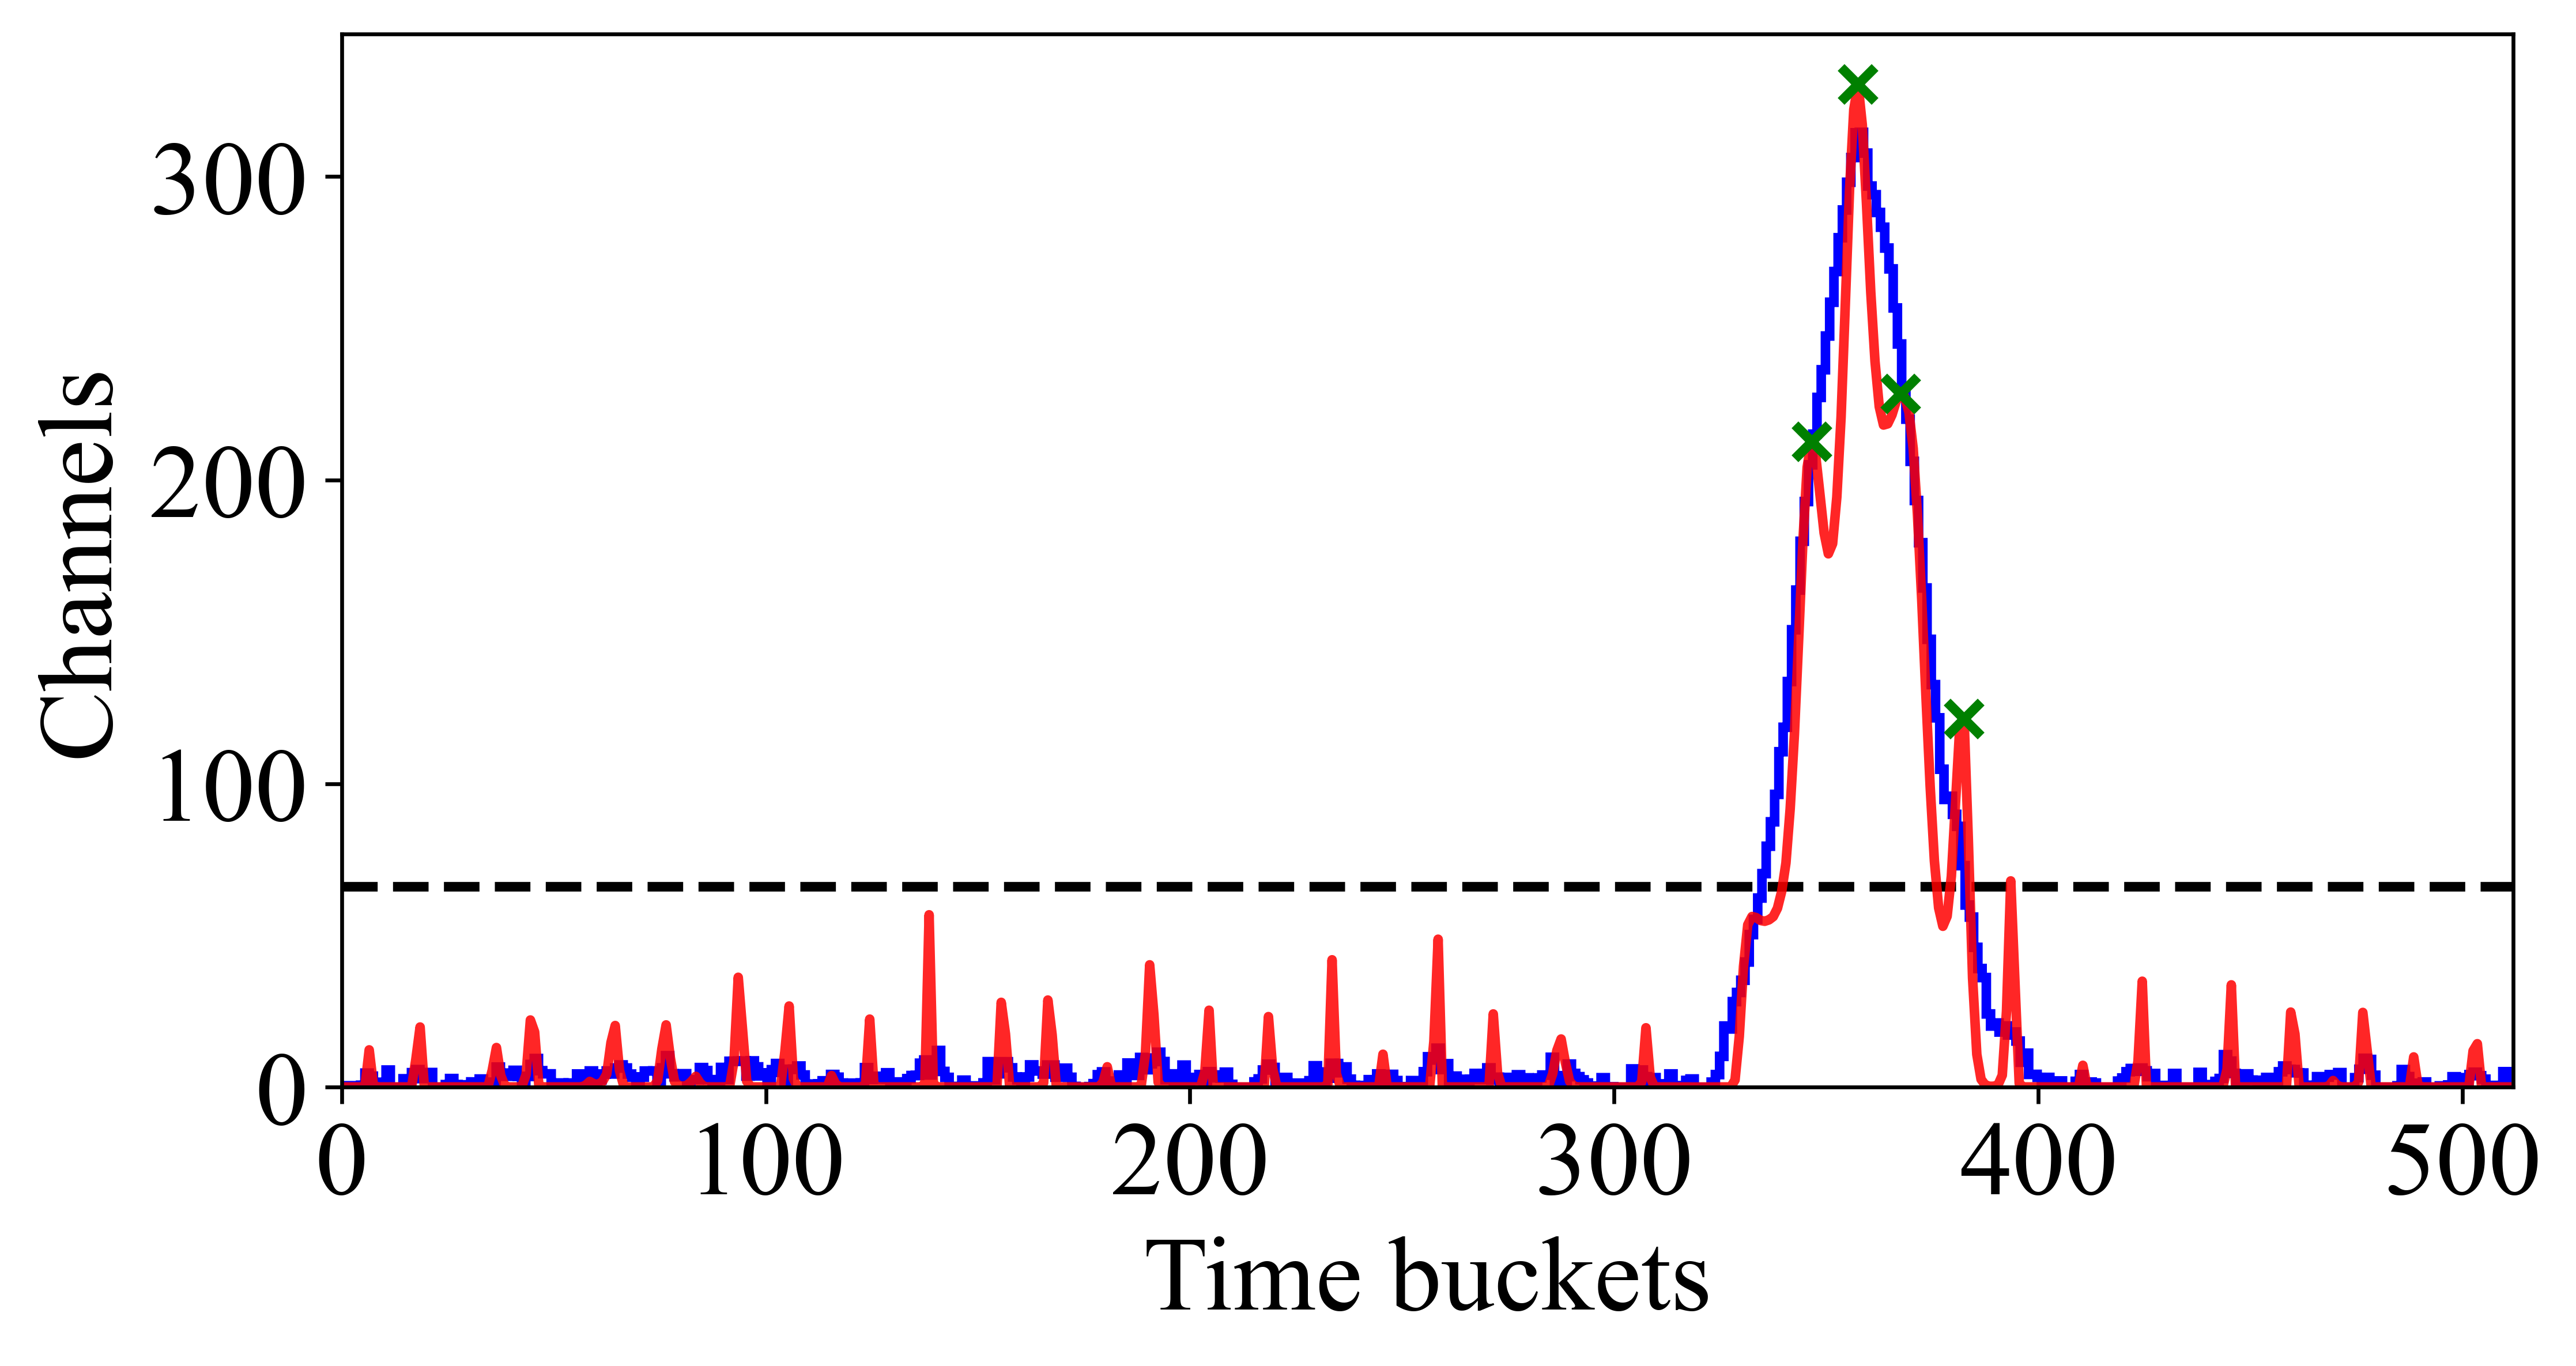
\includegraphics[scale=0.40]{figs/ex_deconv_2.png}
        \caption{}
        \label{subfig:ex_sinal_deconv_2}
    \end{subfigure}
    \begin{subfigure}[b]{0.48\textwidth}
        \centering
        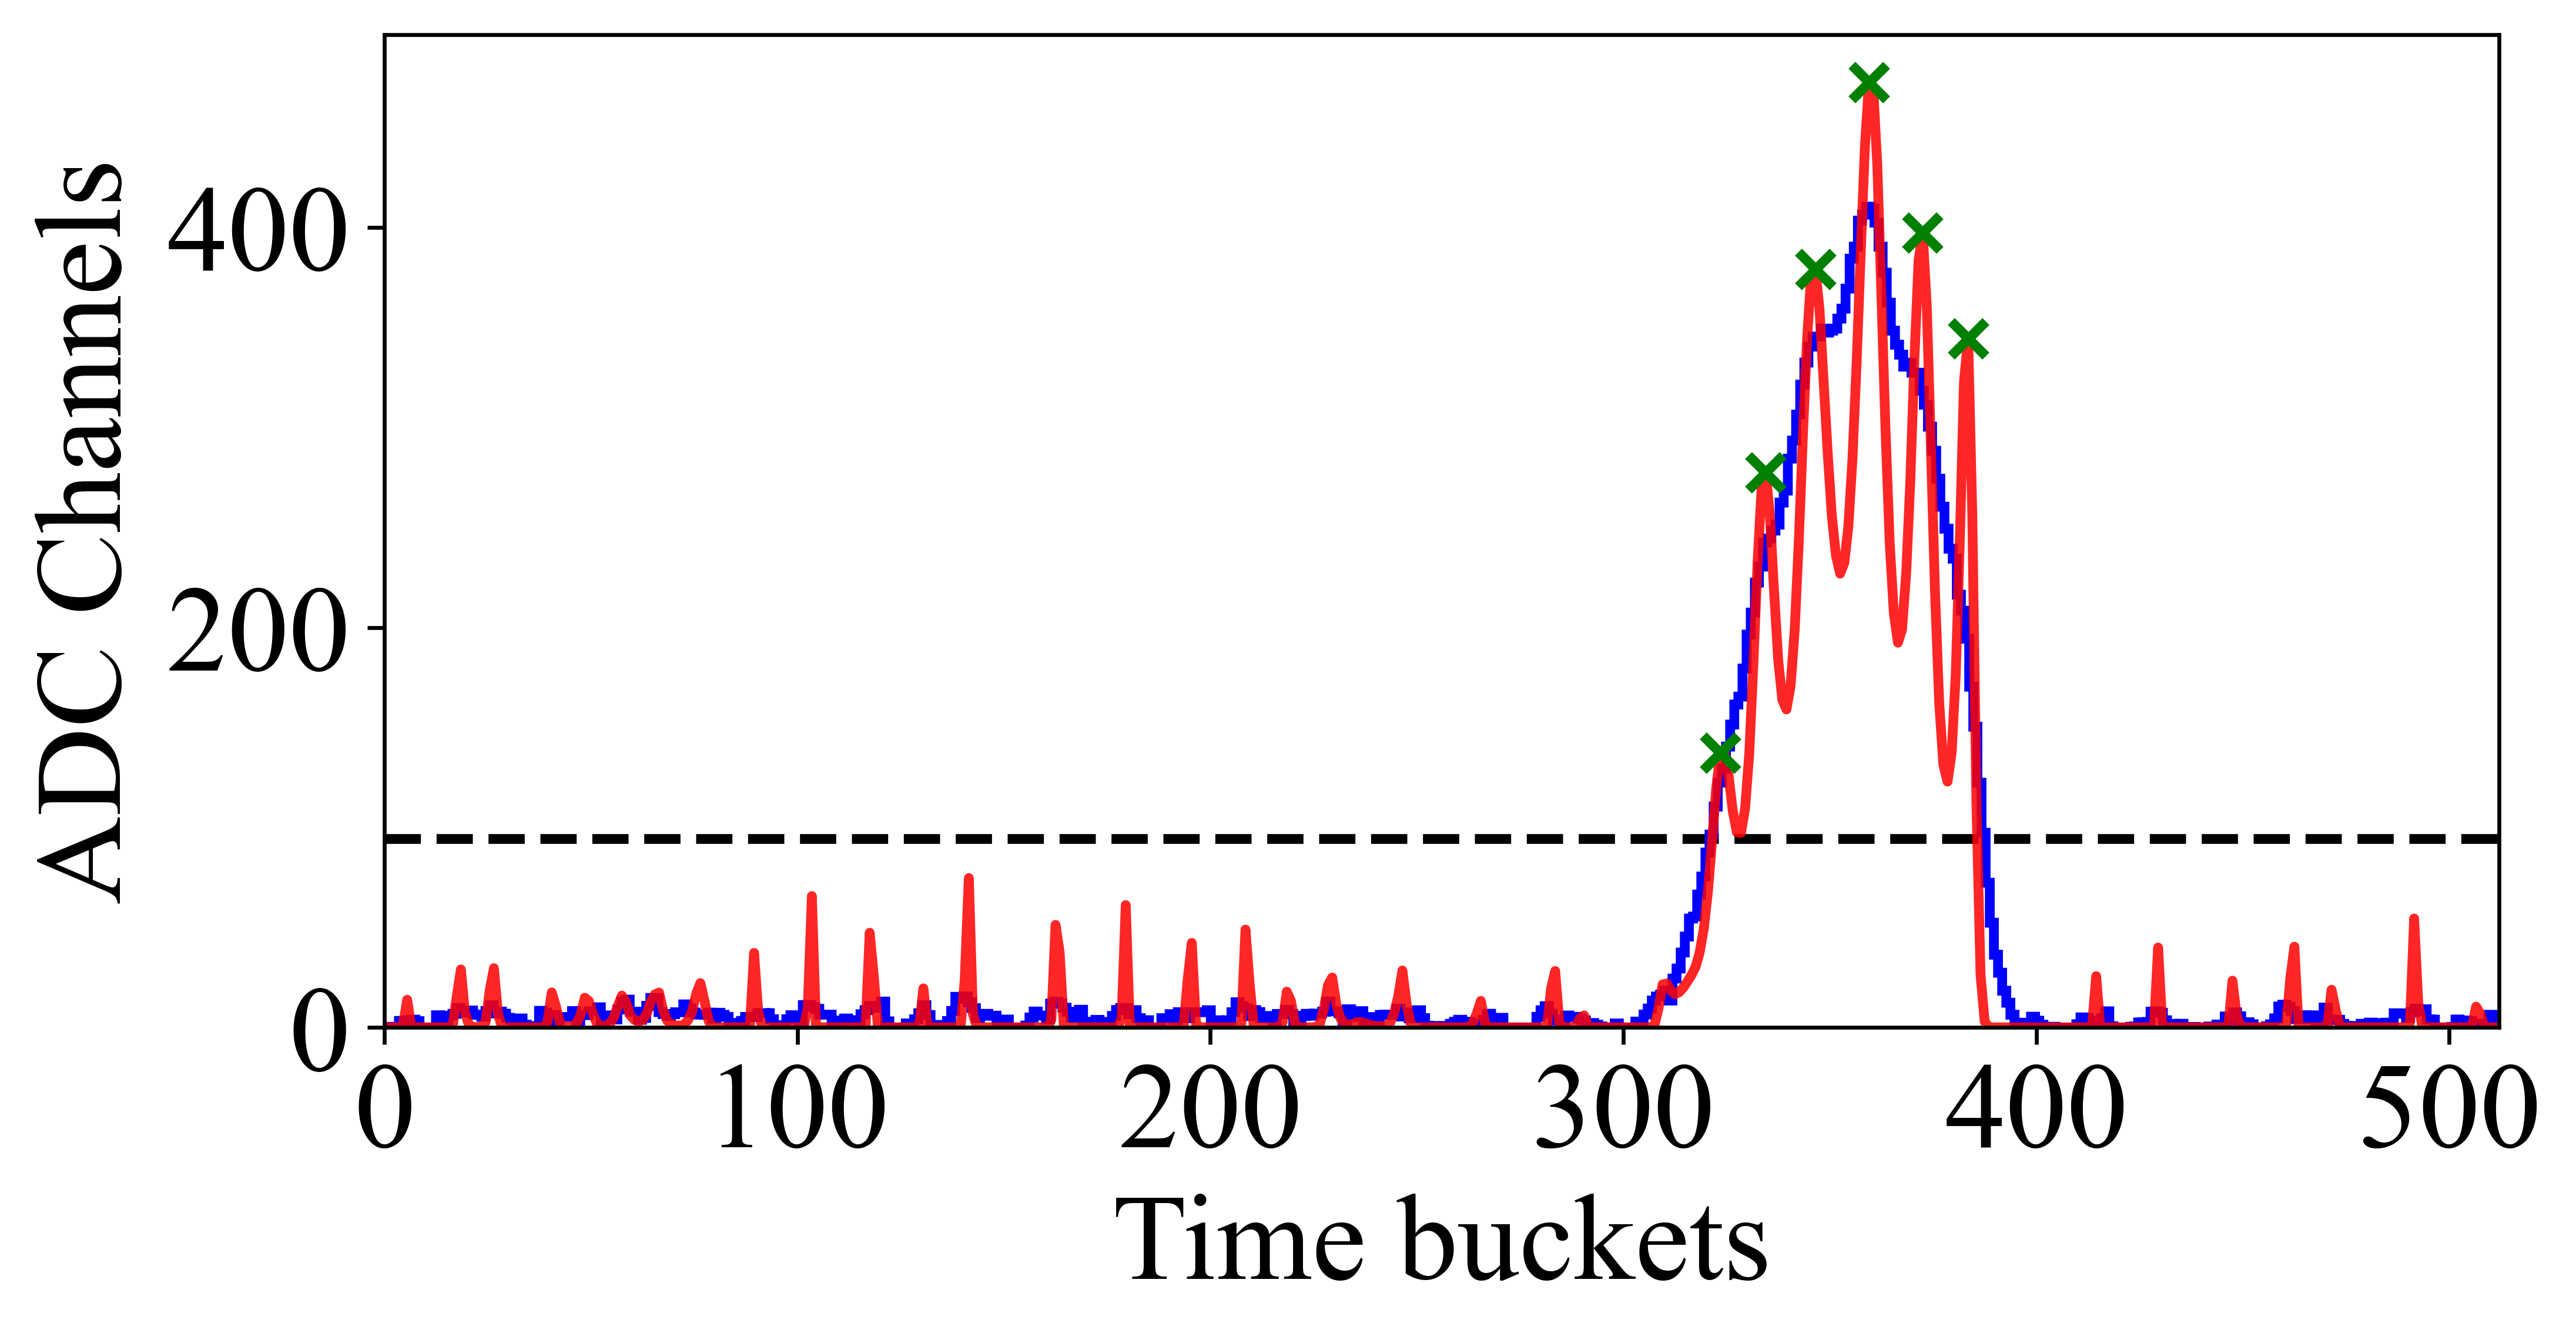
\includegraphics[scale=0.40]{figs/ex_deconv_3.png}
        \caption{}
        \label{subfig:ex_sinal_deconv_3}
    \end{subfigure}%
    \hfill
    \begin{subfigure}[b]{0.48\textwidth}
        \centering
        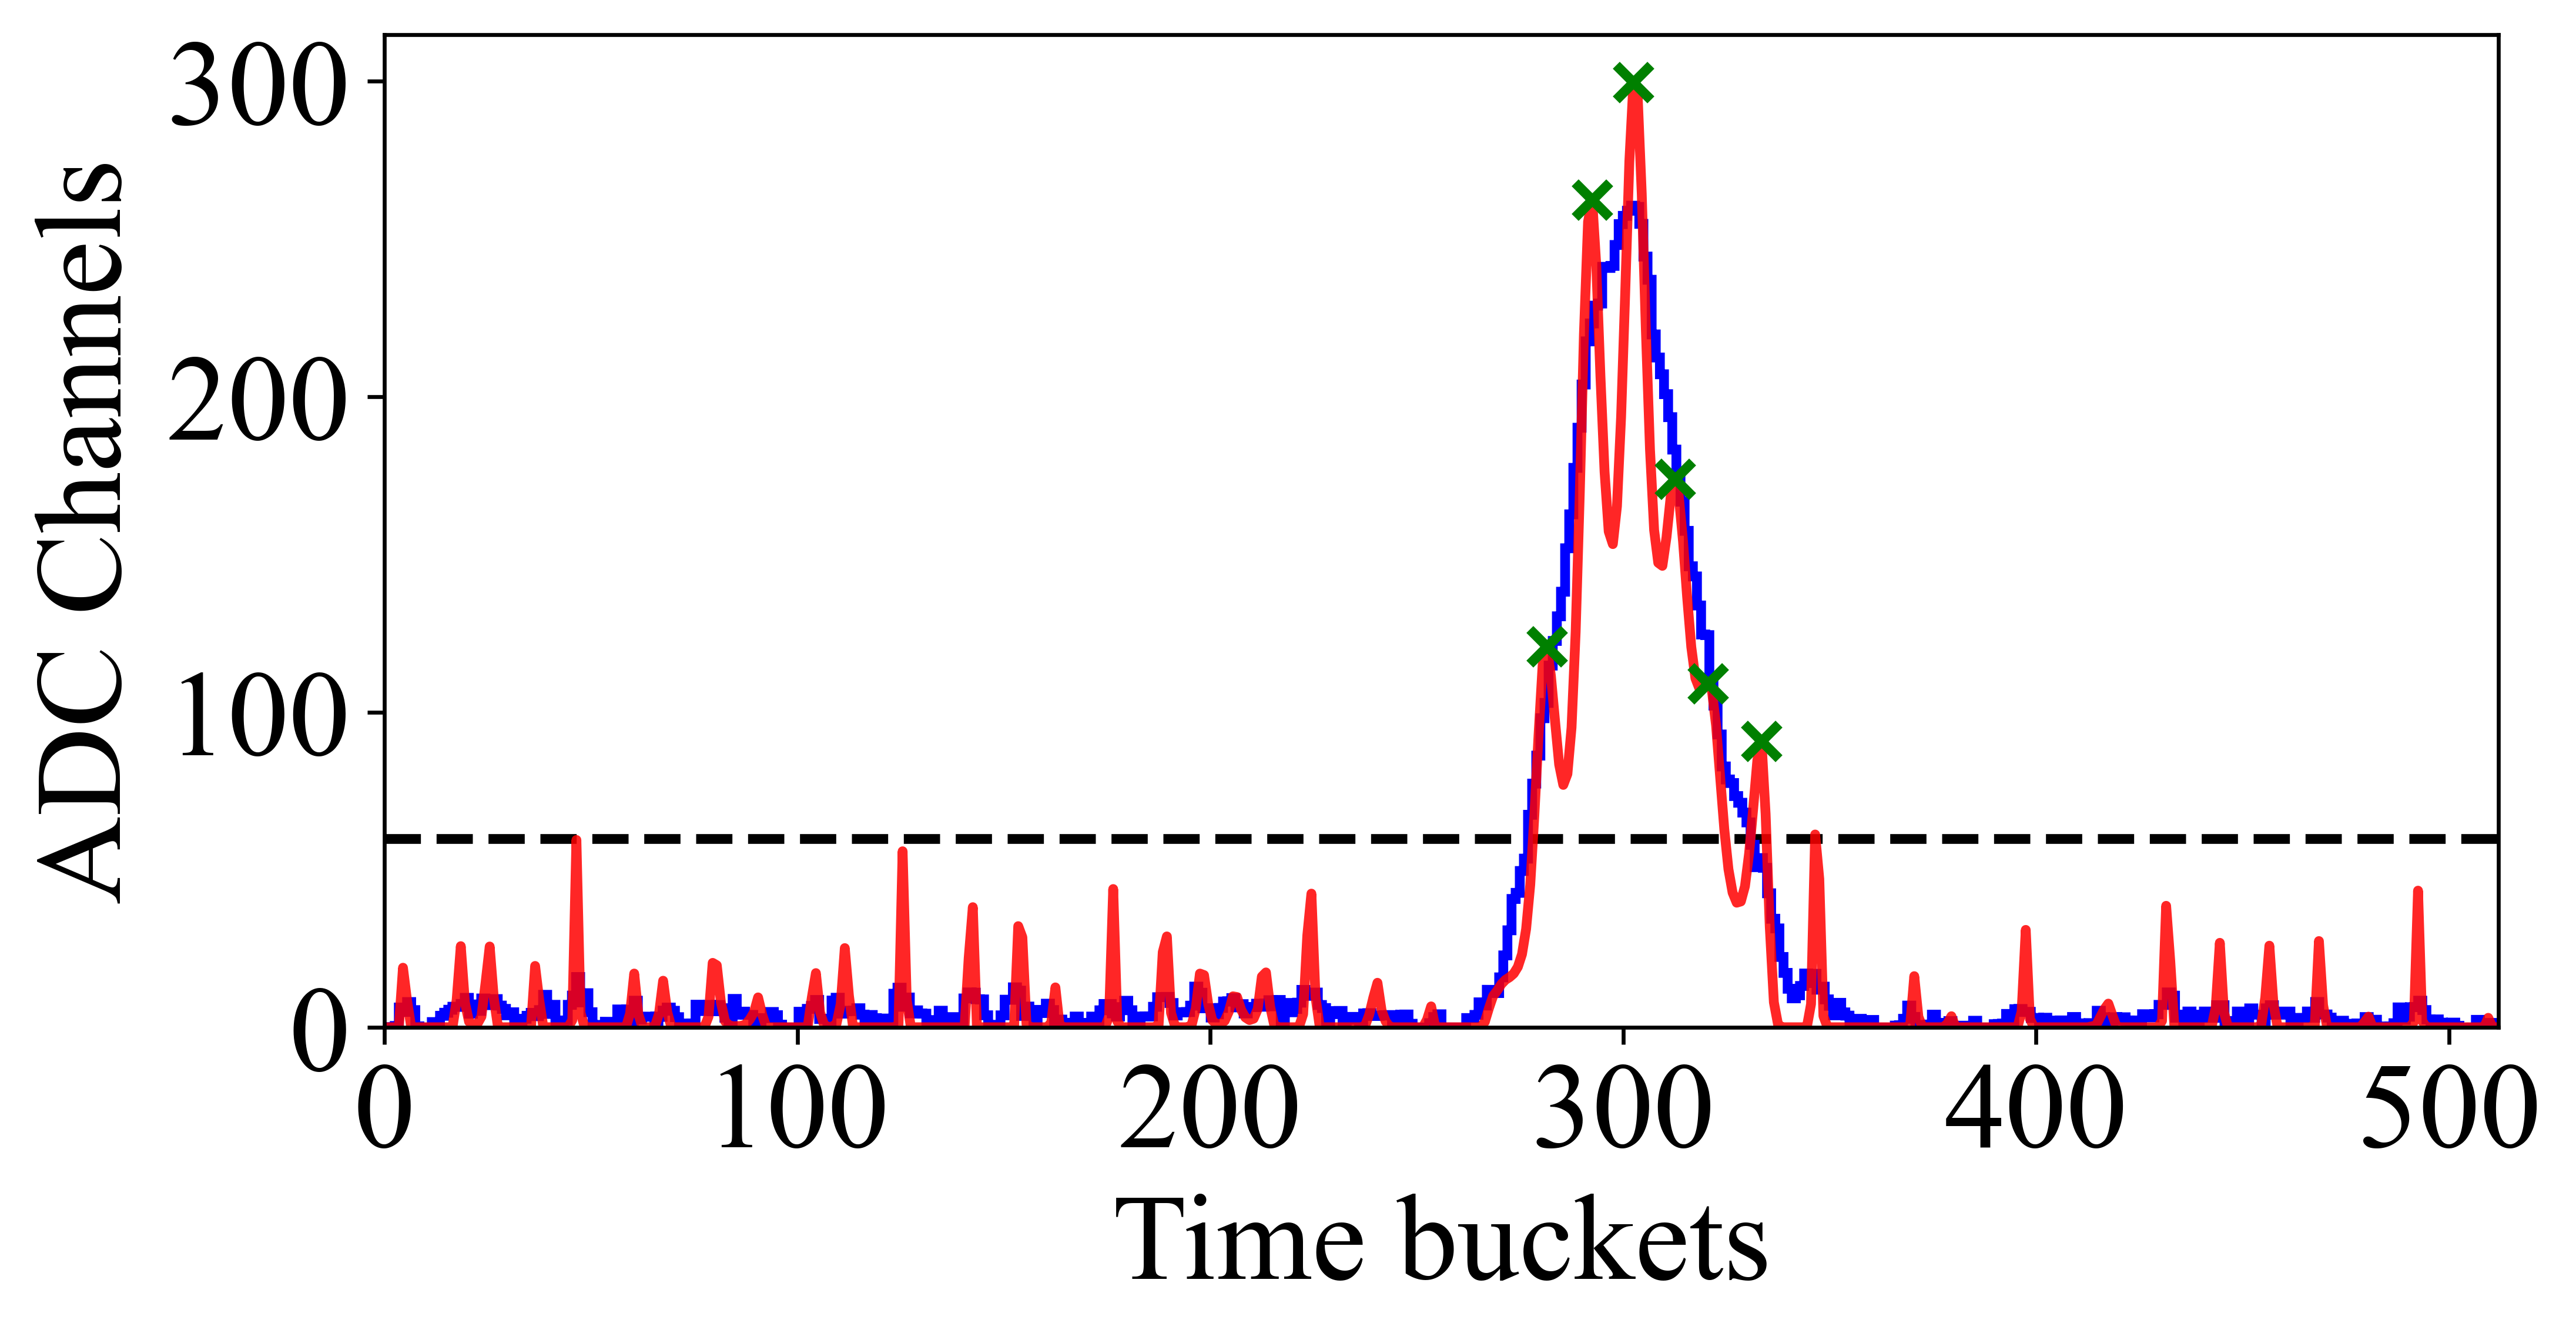
\includegraphics[scale=0.40]{figs/ex_deconv_4.png}
        \caption{}
        \label{subfig:ex_sinal_deconv_4}
    \end{subfigure}
\caption{Histogramas sem as \textit{baselines} antes (em azul) e depois da deconvolução (em vermelho). Os picos (em verde) e o limiar (linha tracejada preta) de identificação também estão indicados.}
\label{fig:ex_sinal_deconv}
\end{figure}

\par O algoritmo de deconvolução também determina a posição dos centróides encontrados, que indica a localização de um pico. Os mesmos picos podem ser obtidos com o \textsc{peak\_finder}, com a vantagem de que o algoritmo possui muitos parâmetros diferentes para calibração, melhorando a identificação em comparação com os picos identificados pelo algoritmo do TSpectrum. A execução de 200.000 sinais, desde a estimativa e remoção do fundo, até a identificação dos centróides, demora cerca de 23,25 minutos, usando o processador Ryzen 5 3600X.

\par Para determinar a carga acumulada $Q$ de cada ponto, é necessário calcular a área do centróide do pico identificado. A área do sinal antes e depois da deconvolução é a mesma, portanto pode-se analisar diretamente o sinal após a deconvolução. Para determinar a área do pulso consideramos a integral simples gaussiana usando a largura de cada pico após a deconvolução. O desvio padrão (largura) dos picos após a deconvolução foi $\sigma_{dd}$ = $1,1543~(44)$ \textit{time buckets}. Considerando esse desvio, a carga integrada para cada ponto é dada por:

%Para achar a área do pulso, foi calculada a largura dos pulsos após a deconvolução, para determinar a área como uma simples integral gaussiana. O desvio padrão dos pulsos após a deconvolução é $\sigma_{dd}$ = 1.1543 (44) time buckets. Com isso foi calculada a carga acumulada para cada ponto medido do evento. A carga acumulada $Q$ para cada ponto $i$ é dada por:

\begin{equation}\label{eq:gauss_area}
    Q = \int^\infty _{-\infty} Ae^{-(t' - t_i)^2 / 2\sigma_{dd}^2} dt' = A\left |\sigma_{dd} \right|\sqrt{2\pi},
\end{equation}
%
onde $A$ é a amplitude do ponto com centróide $t_i$ e desvio padrão após a deconvolução $\sigma_{dd}$. Com o banco de dados para a deconvolução e também para a identificação de picos, basta criar as redes neurais, que serão descritas na seção \ref{sec:pulsos_ml}.

\section{Análise dos pulsos com \textit{machine learning}}\label{sec:pulsos_ml}

\par Com machine learning tem-se a possibilidade de criar algoritmos de alta complexidade sem definir operações explícitas. Usando os resultados das seções anteriores foram desenvolvidas três redes neurais, com o objetivo de: estimar o fundo (subseção \ref{subsec:pulso_ml_fundo}), fazer a deconvolução (\ref{subsec:pulso_ml_deconv}) e por fim identificar os picos (subseção \ref{subsec:pulso_ml_peaks}). 

%Os resultados dos algoritmos usados nas subseções \ref{subsec:pulses_baseline} e \ref{subsec:pulses_deconv} foram usados como \textit{outputs} para o aprendizado das redes neurais que foram desenvolvidas em cada etapa.

\subsection{Rede neural para o fundo}\label{subsec:pulso_ml_fundo}

\par O objetivo foi criar uma rede neural que reproduza o comportamento do algoritmo \textsc{background removal} que estima o fundo do sinal, discutido na seção \ref{subsec:pulses_baseline}. A rede neural é supervisionada, onde os dados de entrada são os sinais brutos e as saídas devem ser os fundos de cada sinal. A arquitetura dessa rede neural é apresentada esquematicamente na figura \ref{fig:arq_source_to_bkg}.

% \par Estimar o fundo é uma tarefa muito complexa pois a eletrônica do detector faz com que o sinal do canal varie muito dependendo do evento, podendo muitas vezes fazer com que o fundo tenha saltos no espectro após receber o sinal de um pulso. Importante ressaltar que a retirada do fundo não precisa ser considerada perfeita. O próprio algoritmo analítico de remoção de fundo não é perfeito e no geral nunca coloca toda a parte que não é o pulso em 0, há muitas flutuações. O importante é tentar deixar o mais próximo de zero possível. 

% \par Estimar o fundo é uma tarefa muito complexa pois ele não é analítico, podendo muitas vezes fazer com que o fundo tenha saltos em diferentes \textit{time buckets}. 

\begin{figure}[H]
    \centering
    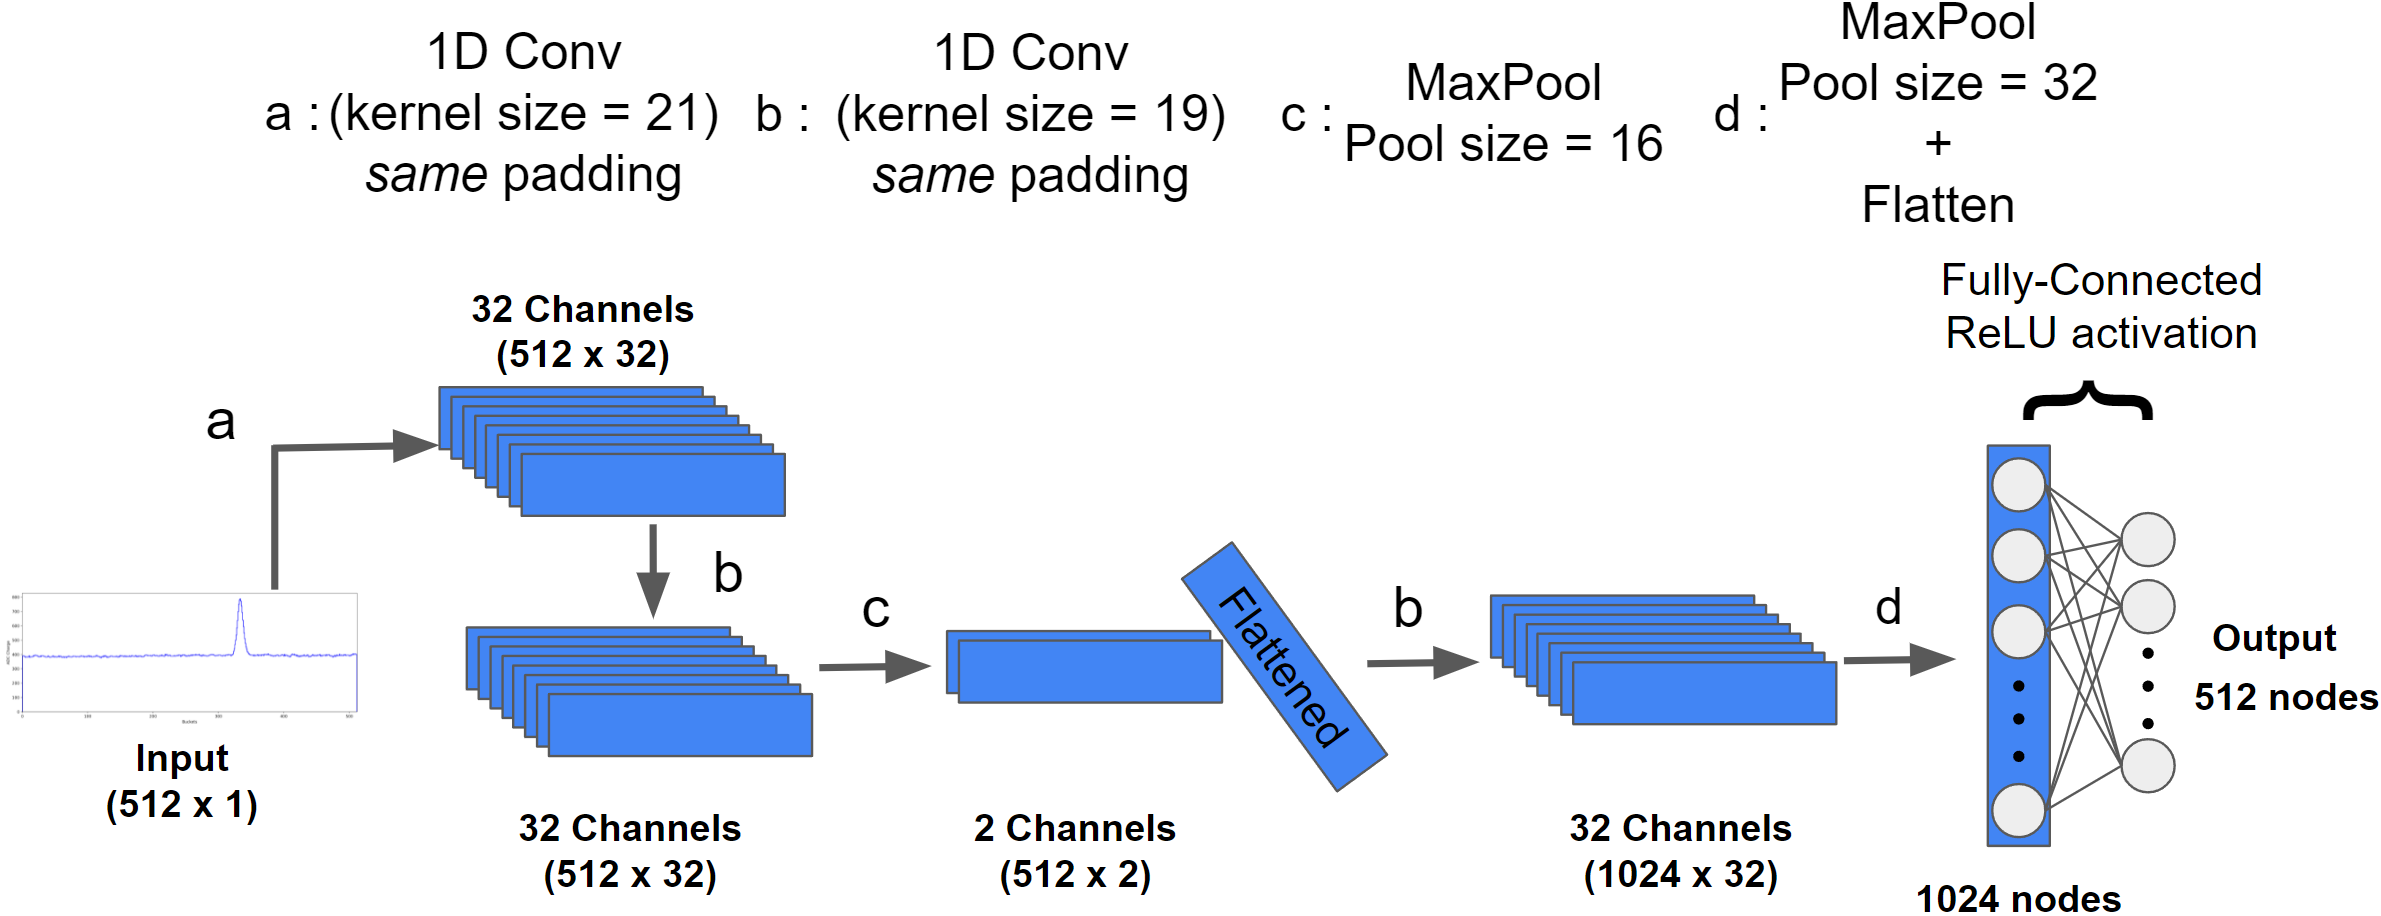
\includegraphics[scale = 0.238]{figs/Source to only bkg.png}
    \caption{Arquitetura da rede neural que faz a inferência do fundo. O vetor de entrada deve ter dimensionalidade 512 x 1. Todas as partes com convolução não possuem o parâmetro \textit{bias}, pois sua presença não mostrou melhora nos resultados da rede neural.}
    \label{fig:arq_source_to_bkg}
\end{figure}

\par Tipicamente, CNNs consistem em um número de camadas convolucionais, eventualmente intercaladas com camadas \textit{Max-Pooling}, e seguidas no final por um número de camadas \textit{fully connected} (FC). Uma camada convolucional consiste de $k$ filtros onde são computadas as operações de convolução entre o vetor de entrada e cada filtro da camada. A saída da camada convolucional consiste, então, em um conjunto de $k$ sinais filtrados. O efeito resultante da aplicação dos filtros depende do tamanho do filtro e dos seus valores; um filtro pode, por exemplo, destacar algumas características do sinal de entrada. Logo, os resultados da saída das camadas convolucionais são conhecidos como mapas característicos (\textit{feature maps}). Por exemplo, na rede neural de correção do sinal de fundo, cuja arquitetura está na figura \ref{fig:arq_source_to_bkg}, o sinal de entrada possui dimensão de $512\times 1$, o que significa um sinal com 512 \textit{time buckets}, enquanto que a saída da camada convolucional possui dimensão de $512\times 32$, o que significa 32 sinais com 512 \textit{time buckets} (32 mapas característicos, ou também canais). O número de filtros $k$ é determinado empiricamente de forma à otimizar a performance da rede neural.

\par O tamanho dos filtros foram escolhidos entre 17 e 21 \textit{time buckets} para cobrir totalmente a região com o pico. Importante notar que, pelo tamanho finito do sinal, não é possível aplicar a operação de convolução nas extremidades do sinal de entrada (primeiros e últimos pontos). Nas camadas convolucionais, se o sinal de saída precisa ser igual ao de entrada, então é escolhido o \textit{same padding} (quando são adicionados zeros nas extremidades do sinal de entrada, de forma que a operação de convolução ocorra e o sinal resultante possua o mesmo tamanho do sinal de entrada).

\par \textit{Max Pooling} é outra operação comum em CNNs. Seu efeito principal é de reduzir a dimensionalidade dos dados por meio de um processo baseado em uma janela com dado valor de seleção (chamado de \textit{pooling size}), selecionando sempre o maior dentre os valores possíveis de cada amostra. A seleção pode ser aplicada com respeito à dimensão dos \textit{time buckets} dos sinais, assim como pode ser aplicada em respeito à dimensão dos canais. No nosso caso, o \textit{pool size} escolhido foi 16 para reduzir o número de canais de 32 para 2. Isso reduz o número de parâmetros e consequentemente o tempo de treino. No final da rede neural, algumas camadas FC foram incluídas. Entre a última camada convolucional e a primeira camada FC foi aplicado uma planificação (ou \textit{flat}) para diminuir a dimensionalidade da dimensão dos canais de 2 para 1.  Na camada final, foi usada a função de ativação ReLU ($f(x) = \max(0, x)$) para garantir o valor mínimo em zero e para prevenir problemas com a minimização da função custo \cite{VGP}. A função de ativação ReLU também é não linear que ajuda a rede neural a aprender operações não lineares, assim como no nosso caso.

%\par A entrada da rede é o sinal ``cru" com dimensionalidade 521 x 1. A seguir realizamos duas convoluções (passagens \textit{a} e \textit{b}) com padding same e uma camada com Max pooling, a fim de diminuir o número de canais resultente. Os dois canais restantes sofrem uma planificação (ou flat), diminuindo sua dimensionalidade, para então passar por mais uma convolução com padding same e filtros de tamanho 19 seguido de uma camada Max pooling, para deixar apenas um canal resultante, para enfim passar pela última camada Fully Connected com função de ativação ReLU. Toda a rede neural foi construída usando o TensorFlow 2 e possui um total de 545.536 parâmetros, todos treináveis. O tamanho dos filtros das convoluções levam em conta a largura do pulso, sendo no mínimo um valor maior que a largura, a fim de que cada kernel de cada convolução atue em um pulso completo na convolução \cite{FORTINO2022166497}.

%\par A camada final com função de ativação ReLU garante o valor mínimo de saída em 0 e, principalmente, pelo fato de não causar problemas à minimização do gradiente \cite{VGP}. O processo de criação de arquiteturas de redes neurais é algo que não possui teoria, sendo um processo na maior parte do tempo empírico. Foram testadas diversas combinações e a que está sendo mostrada na figura \ref{fig:arq_source_to_bkg} é a que obteve os melhores resultados \cite{FORTINO2022166497}.

% Caso, por exemplo, na passagem \textit{c} da figura, o \textit{pool size} da camada de \textit{max pooling} fosse 32 (a fim de sobrarem 512 canais igual na entrada e na saída), a rede parece não entender as oscilações grandes do sinal de fundo.
\par Para o treino foram usados 160.000 sinais pré analisados selecionados de forma aleatória. Um conjunto de dados menor de 40.000 sinais pré analisados também foram usados como validação para o modelo treinado. A CNN foi desenvolvida usando o TensorFlow 2 com mais de meio milhão de parâmetros treináveis. O treino foi realizado usando a GPU (graphics processing unit) NVIDIA Tesla P100 e durou cerca de 1 hora. O loss foi escolhido como sendo o erro quadrático médio, dado por

\begin{equation}\label{eq:erro_quad_m}
    E = \frac{1}{N}\sum_{i = 1}^{N} \left( x_i - \Hat{x}_i\right )^2,
\end{equation}
%
onde $E$ é o erro quadrático médio, $N$ é o número de pontos e $x_i$ o ponto da saída da rede para ser comparado com o ponto original $\Hat{x}_i$. O otimizador foi o ADAMAX \cite{ADAMAX}, com learning rate de 0.0005 (parâmetro $\alpha$ da equação \ref{eq:SGD}), e métrica para avaliação foi o erro médio absoluto, dado por

\begin{equation}\label{eq:erro_abs_m}
    E = \frac{1}{N}\sum_{i = 1}^{N} \left | x_i - \Hat{x}_i\right |,
\end{equation}
%
onde $E$ é o erro absoluto médio, $N$ é o número de pontos e $x_i$ o ponto da saída da rede para ser comparado com o ponto original $\Hat{x}_i$. Utilizamos 30 epochs (iterações de treino) e adotamos um batch size de 8. Os resultados do treino são mostrados na figura \ref{fig:source_to_bkg_results}. Como podemos ver na figura, os treinos são bem validados a partir da epoch 20, quando começa um platô no \textit{loss}.

% \par Como dito na seção \ref{sec:ml} temos que especificar qual o tamanho do filtro das camadas convolucionais. Para determinar o fundo precisamos, ponto a ponto, determinar quantos canais na direita e na esquerda o filtro deve atuar. Por exemplo, caso o tamanho do filtro fosse 3, ele só estaria ``enxergando" um ponto à direita e um à esquerda, para então passar a informação a diante, porém claramente é um filtro muito pequeno, as oscilações podem variar mais do que 5 canais. Além disso, quando há o começo de um pulso no sinal, ele pode se estender por múltiplos canais, então é preciso escolher um tamanho de filtro grande o suficiente para enxergar todas essas diferenças. A rede consta com duas camadas convolucionais em sequência com filtros de tamanho 21 e 19, respectivamente.

\begin{figure}[H]
\centering
    \begin{subfigure}[t]{\textwidth}
        \centering
        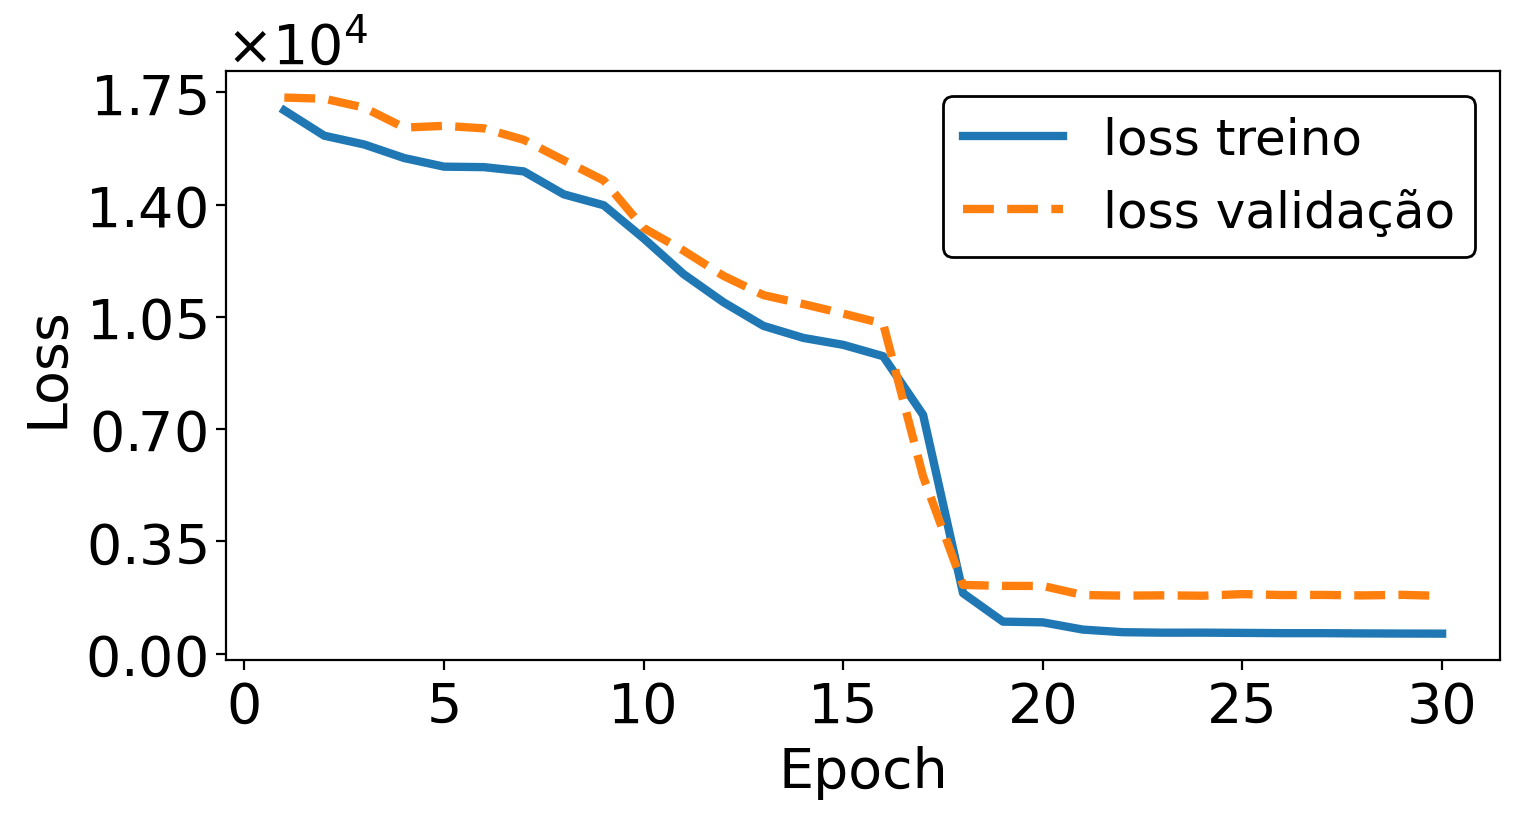
\includegraphics[scale=0.51]{figs/source_to_bkg_loss.png}
        \caption{Loss dos dados de treino (linha contínua) e dos dados de validação (linha tracejada) em função da epoch no treino da rede dada pela figura \ref{fig:arq_source_to_bkg}.}
        \label{subfig:source_to_bkg_loss}
    \end{subfigure}%
    \vfill
    \begin{subfigure}[t]{\textwidth}
        \centering
        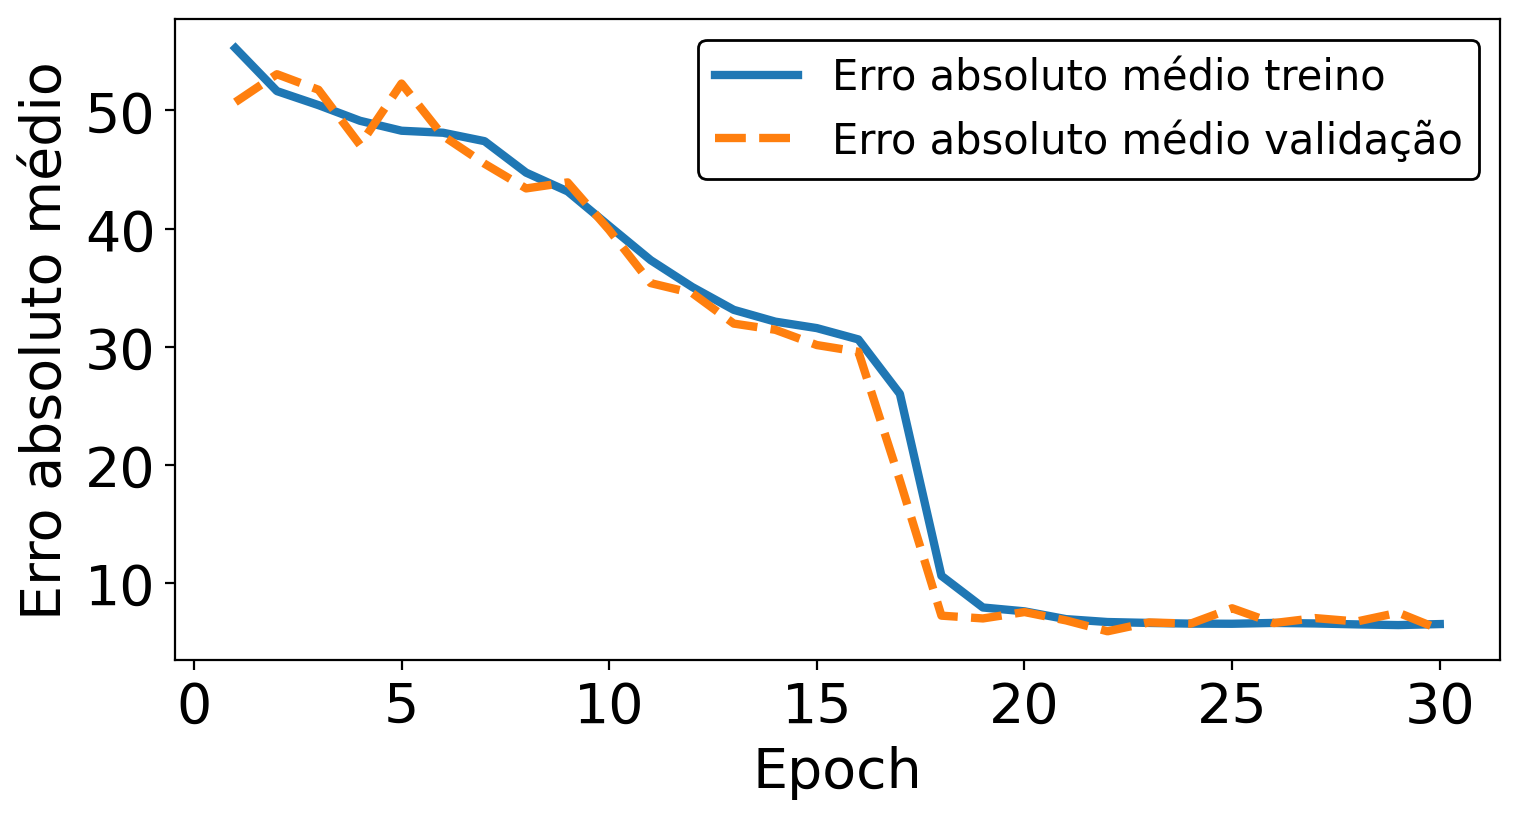
\includegraphics[scale=0.51]{figs/source_to_bkg_metric.png}
        \caption{Erro absoluto médio dos dados de treino (linha contínua) e dos dados de validação (linha tracejada) em função da epoch no treino da rede dada pela figura \ref{fig:arq_source_to_bkg}.}
        \label{subfig:source_to_bkg_metric}
    \end{subfigure}
\caption{Resultados do treino da rede neural representada na figura \ref{fig:arq_source_to_bkg}. A rede atingiu seu melhor resultado a partir da epoch 20.}
\label{fig:source_to_bkg_results}
\end{figure}

% \par A métrica do erro absoluto médio mede ponto a ponto qual o erro absoluto da previsão. 

\par A arquitetura da figura \ref{fig:arq_source_to_bkg} (assim como as próximas desse capítulo) foi determinada de forma empírica. Uma arquitetura com menos passagens e/ou menos parâmetros fornece resultados menos adequados em comparação com a arquitetura apresentada. No caso de mais parâmetros e /ou passagens (consequentemente com aumento no tempo de execução), a rede neural não demonstrou melhora substancial.

\par Exemplos de resultados de previsões da rede neural estão na figura \ref{fig:stb_examples}. A previsão do fundo possui um erro absoluto nos dados de treino de 6.5315 ADC Channels e nos dados de validação de 6.0783 ADC Channels. O sinal cru é subtraído do fundo, colocando o valor mínimo da subtração em 0. O erro médio absoluto de 200.000 sinais sem o respectivo fundo (resultante do algoritmo do TSpectrum) foi estimado em apenas 4.5 ADC Channels.
% Esse erro significa que, por exemplo, para o menor pico detectado considerado, que possui amplitude de cerca de 60 unidades em y, a incerteza estimada da amplitude seria de 7.5\%, ou seja, na menor amplitude possível para um pico a incerteza propagada seria de 7.5\% da amplitude.

\par Rede neurais convolucionais têm a vantagem de usarem poucas variáveis e serem facilmente paralelizadas em sua execução \cite{mlbook}. Uma vantagem de redes neurais é o seu tempo de execução. Empiricamente a rede neural pode processar 200.000 sinais em apenas 8 s (ou 25.000 sinais por segundo), sendo muito eficiente em tempo.

\begin{figure}[H]
\centering
    \begin{subfigure}[b]{0.47\textwidth}
        \centering
        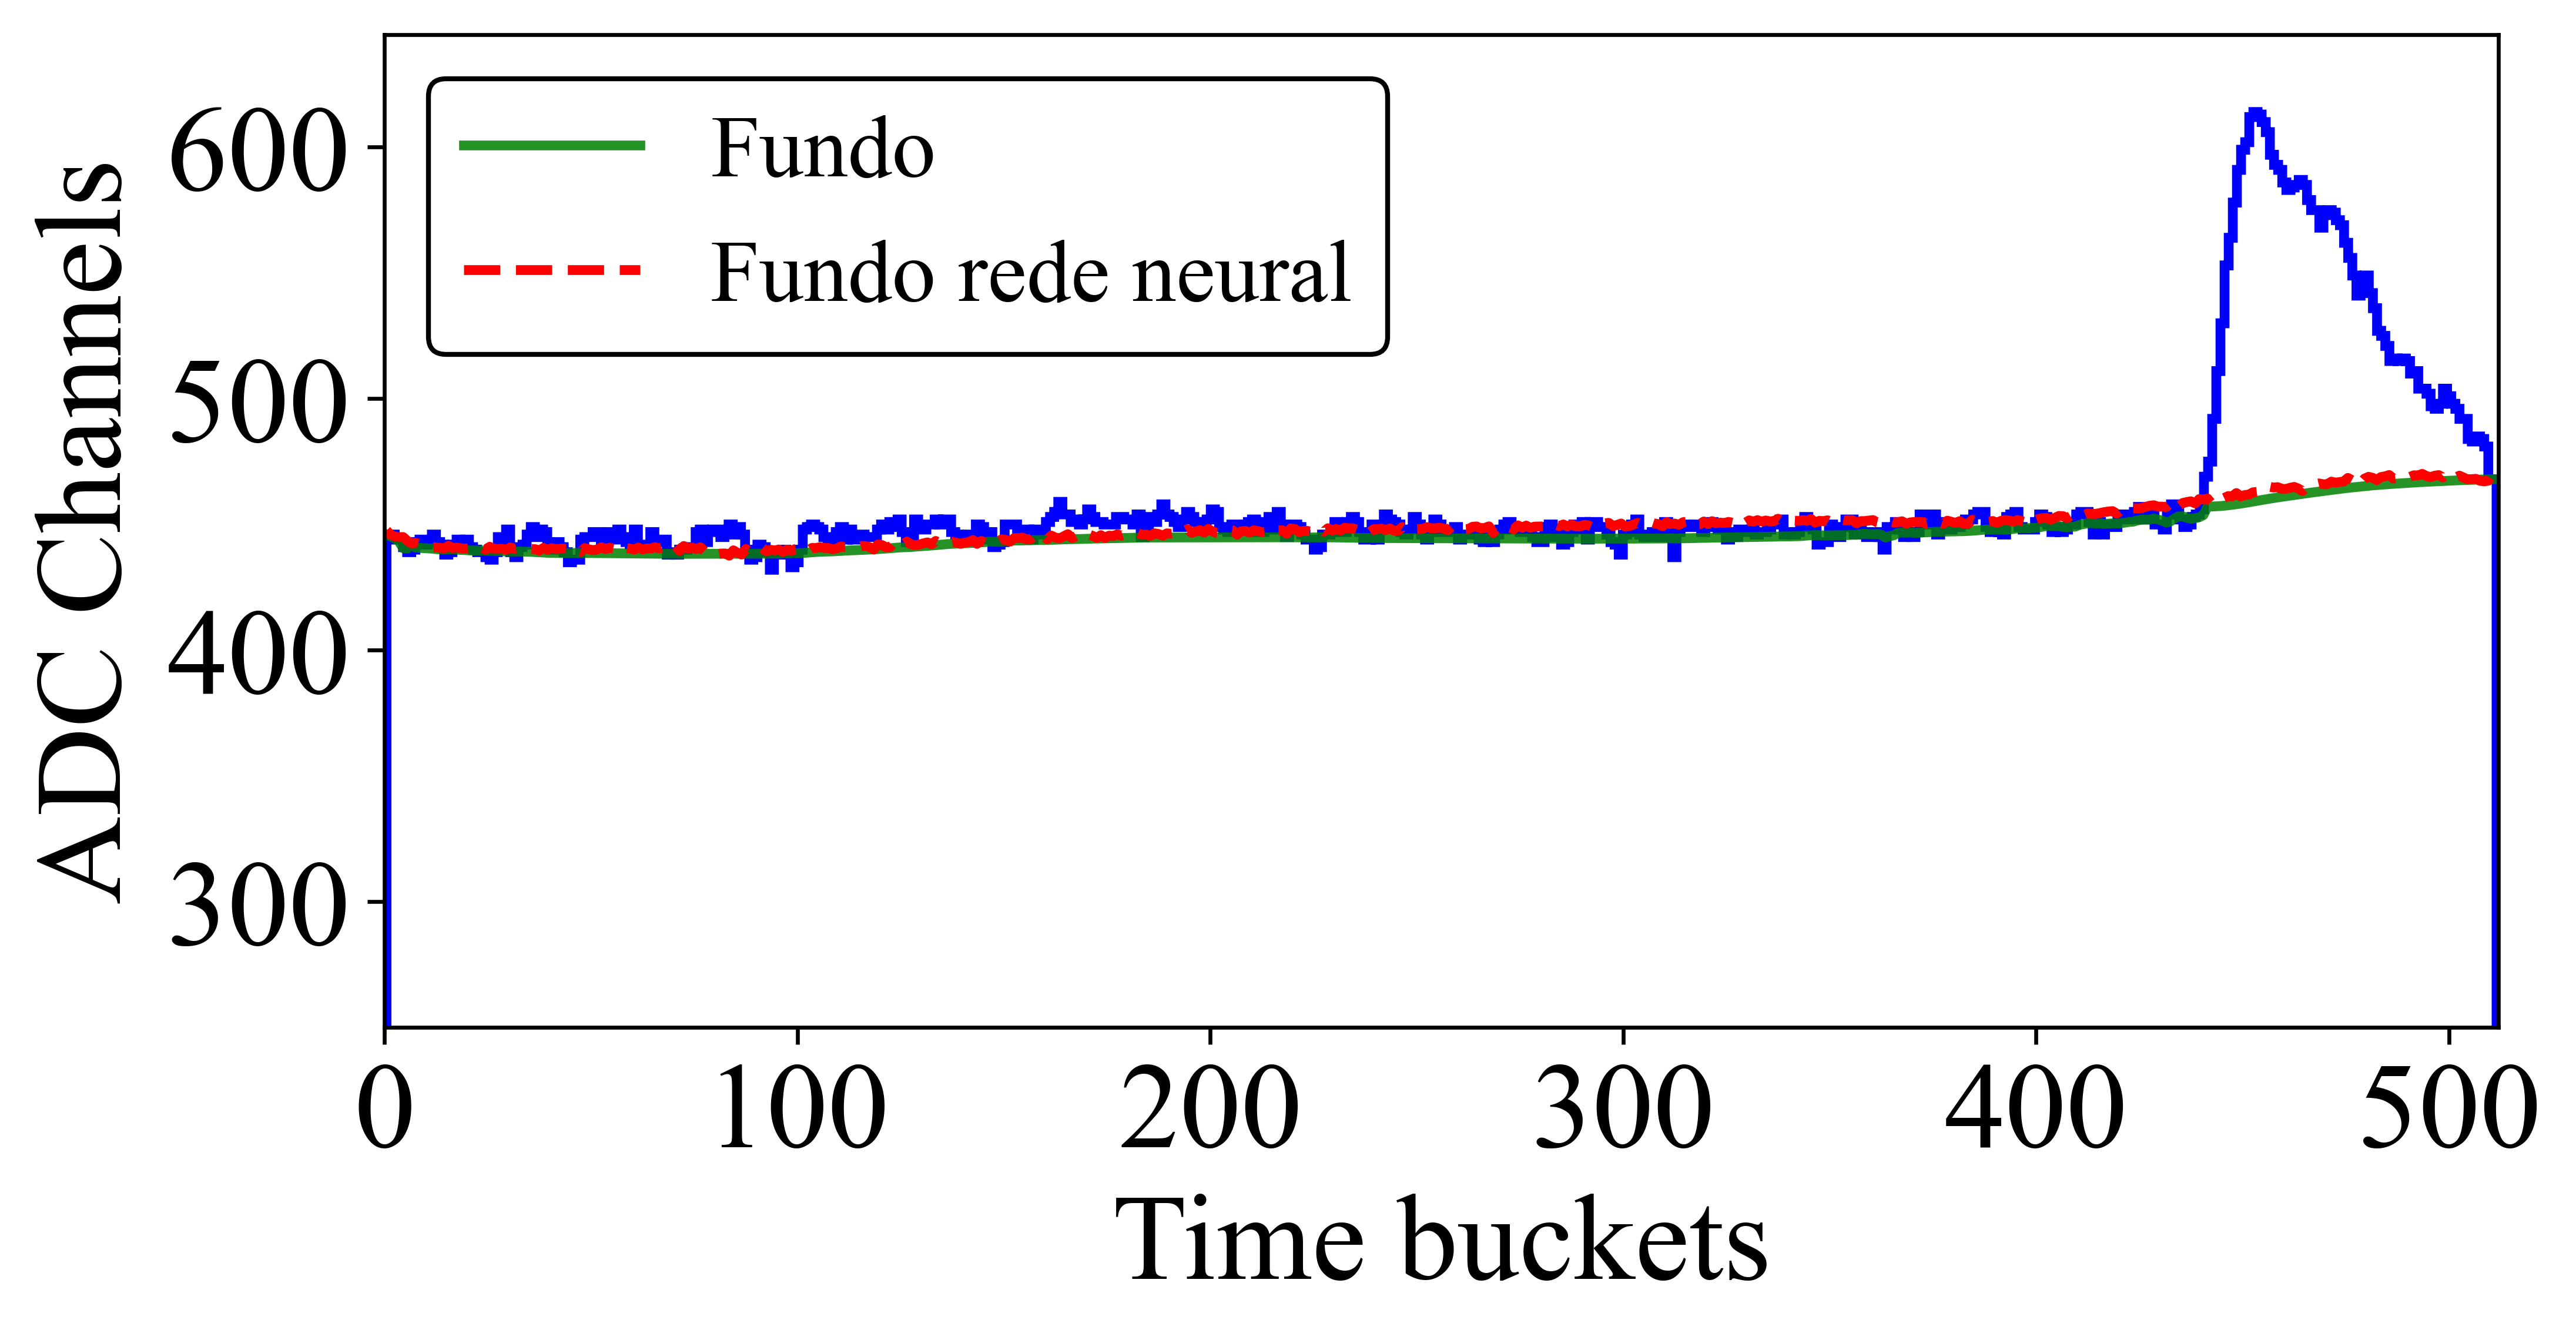
\includegraphics[scale=0.43]{figs/stb_1.png}
        \caption{}
        \label{subfig:stb_ex1}
    \end{subfigure}%
    \hfill
    \begin{subfigure}[b]{0.46\textwidth}
        \centering
        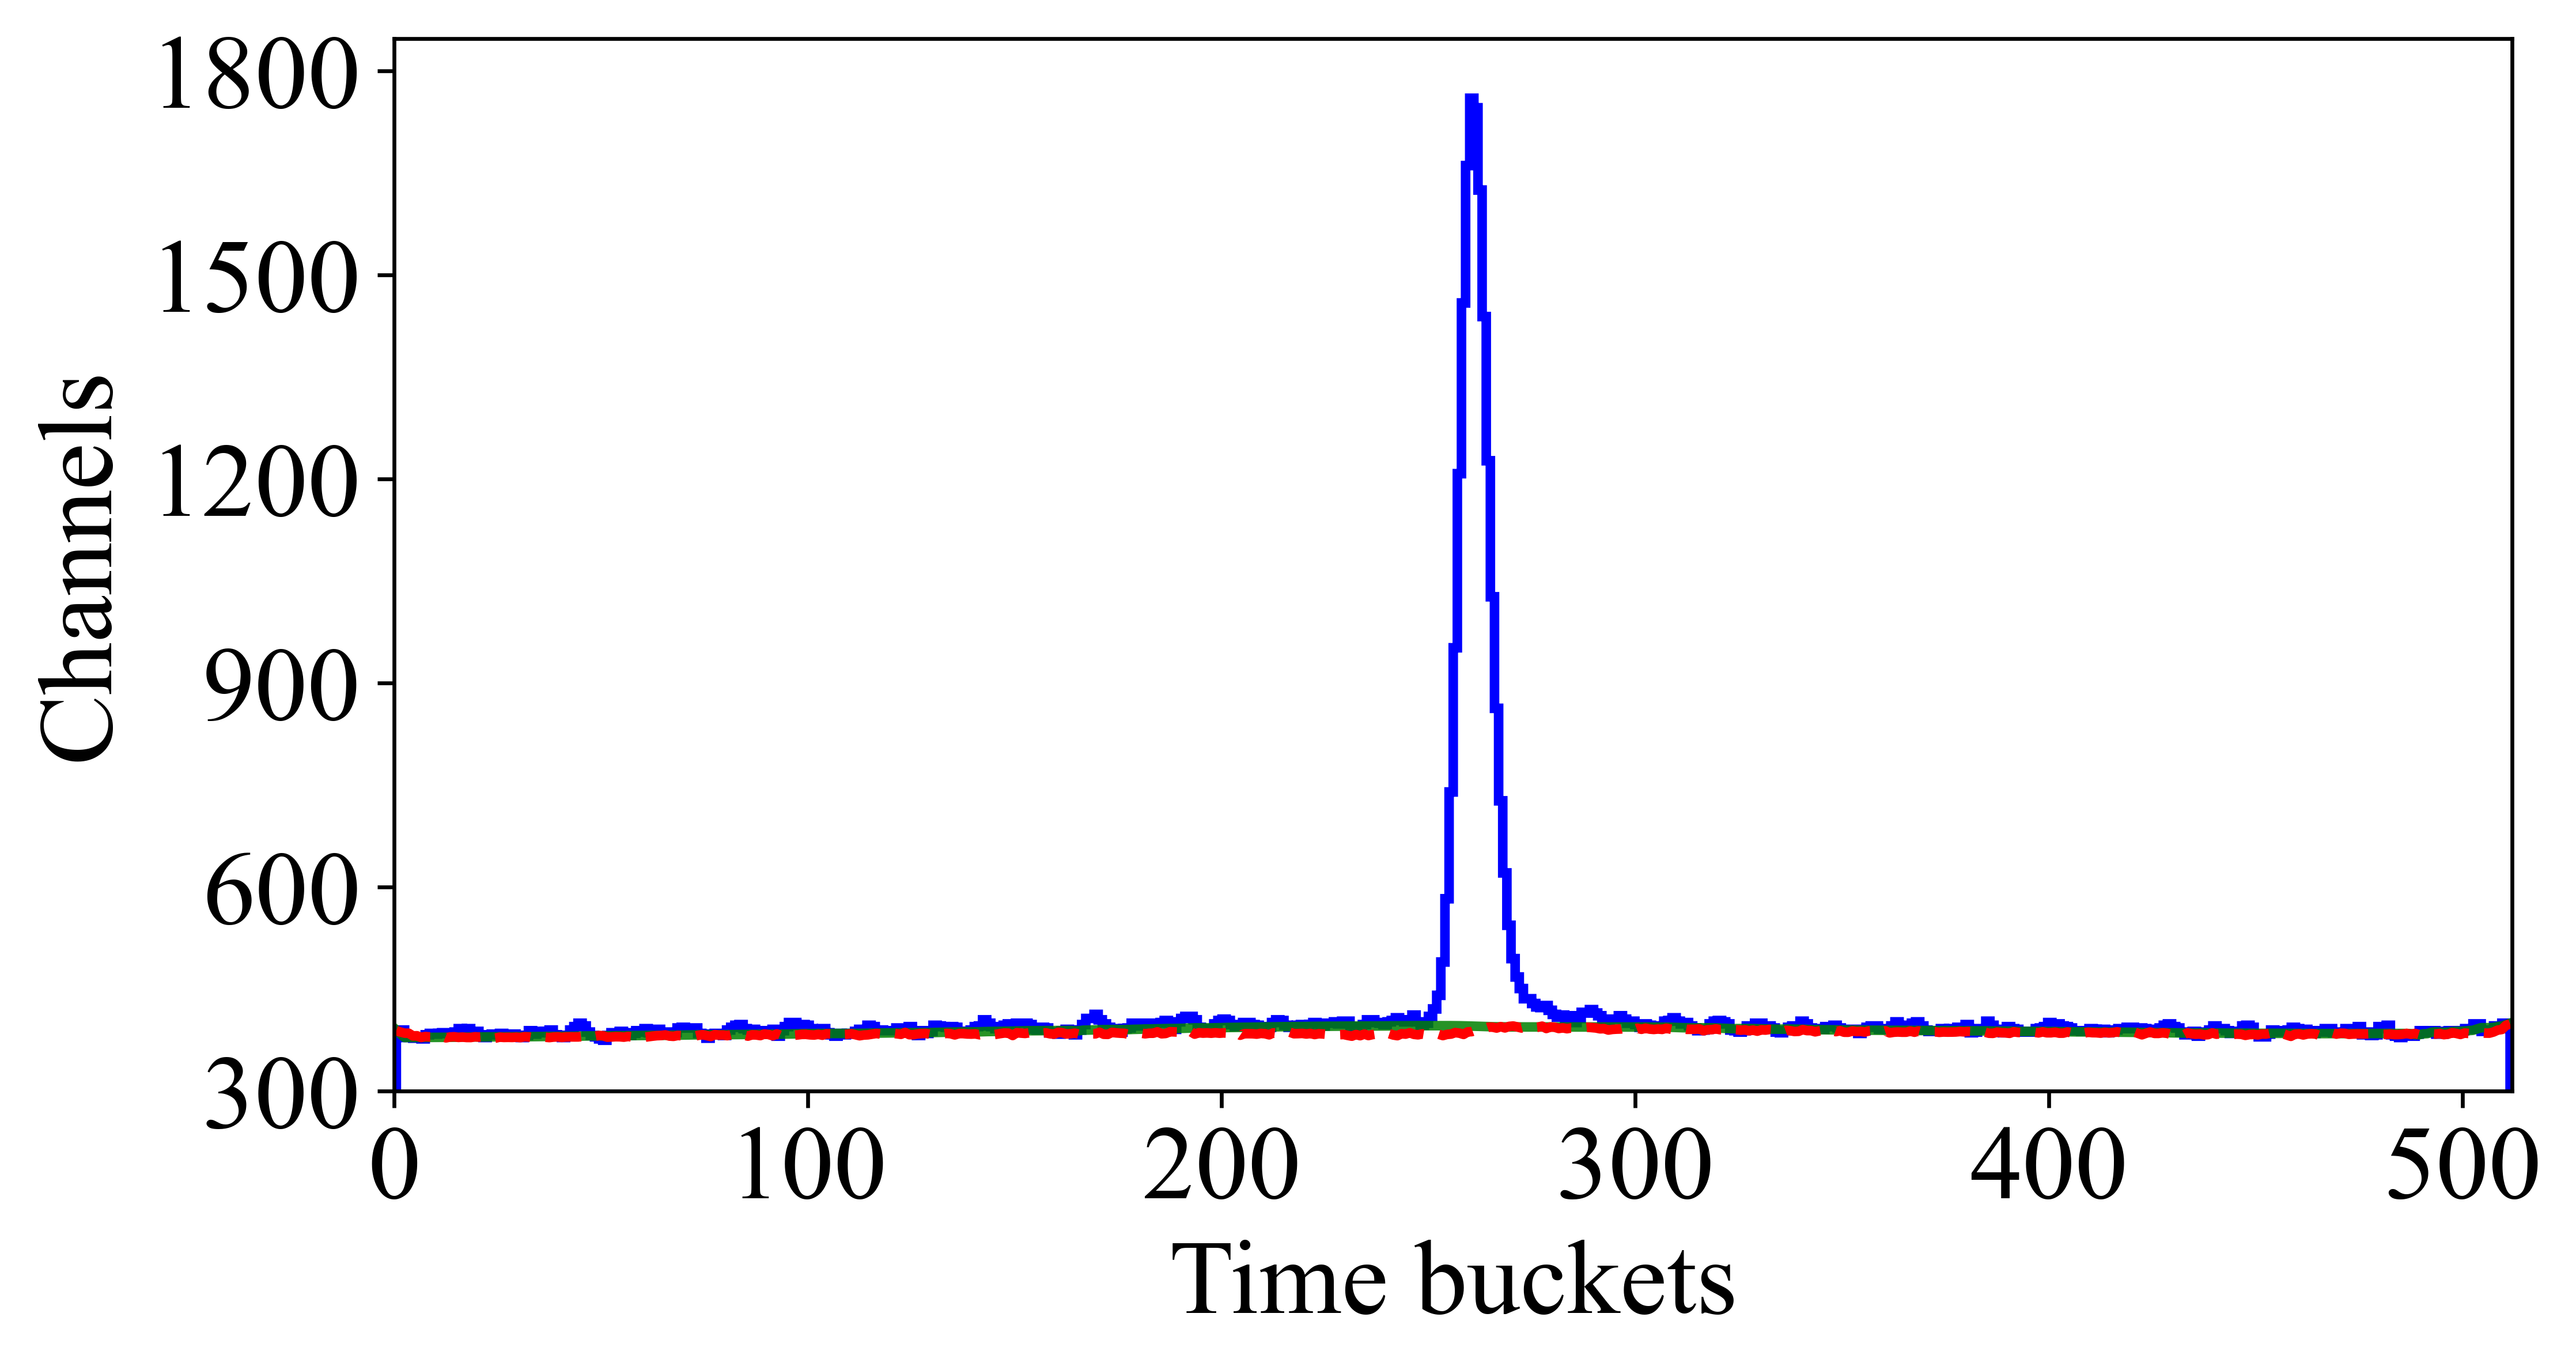
\includegraphics[scale=0.43]{figs/stb_2.png}
        \caption{}
        \label{subfig:stb_ex2}
    \end{subfigure}
    \begin{subfigure}[b]{0.47\textwidth}
        \centering
        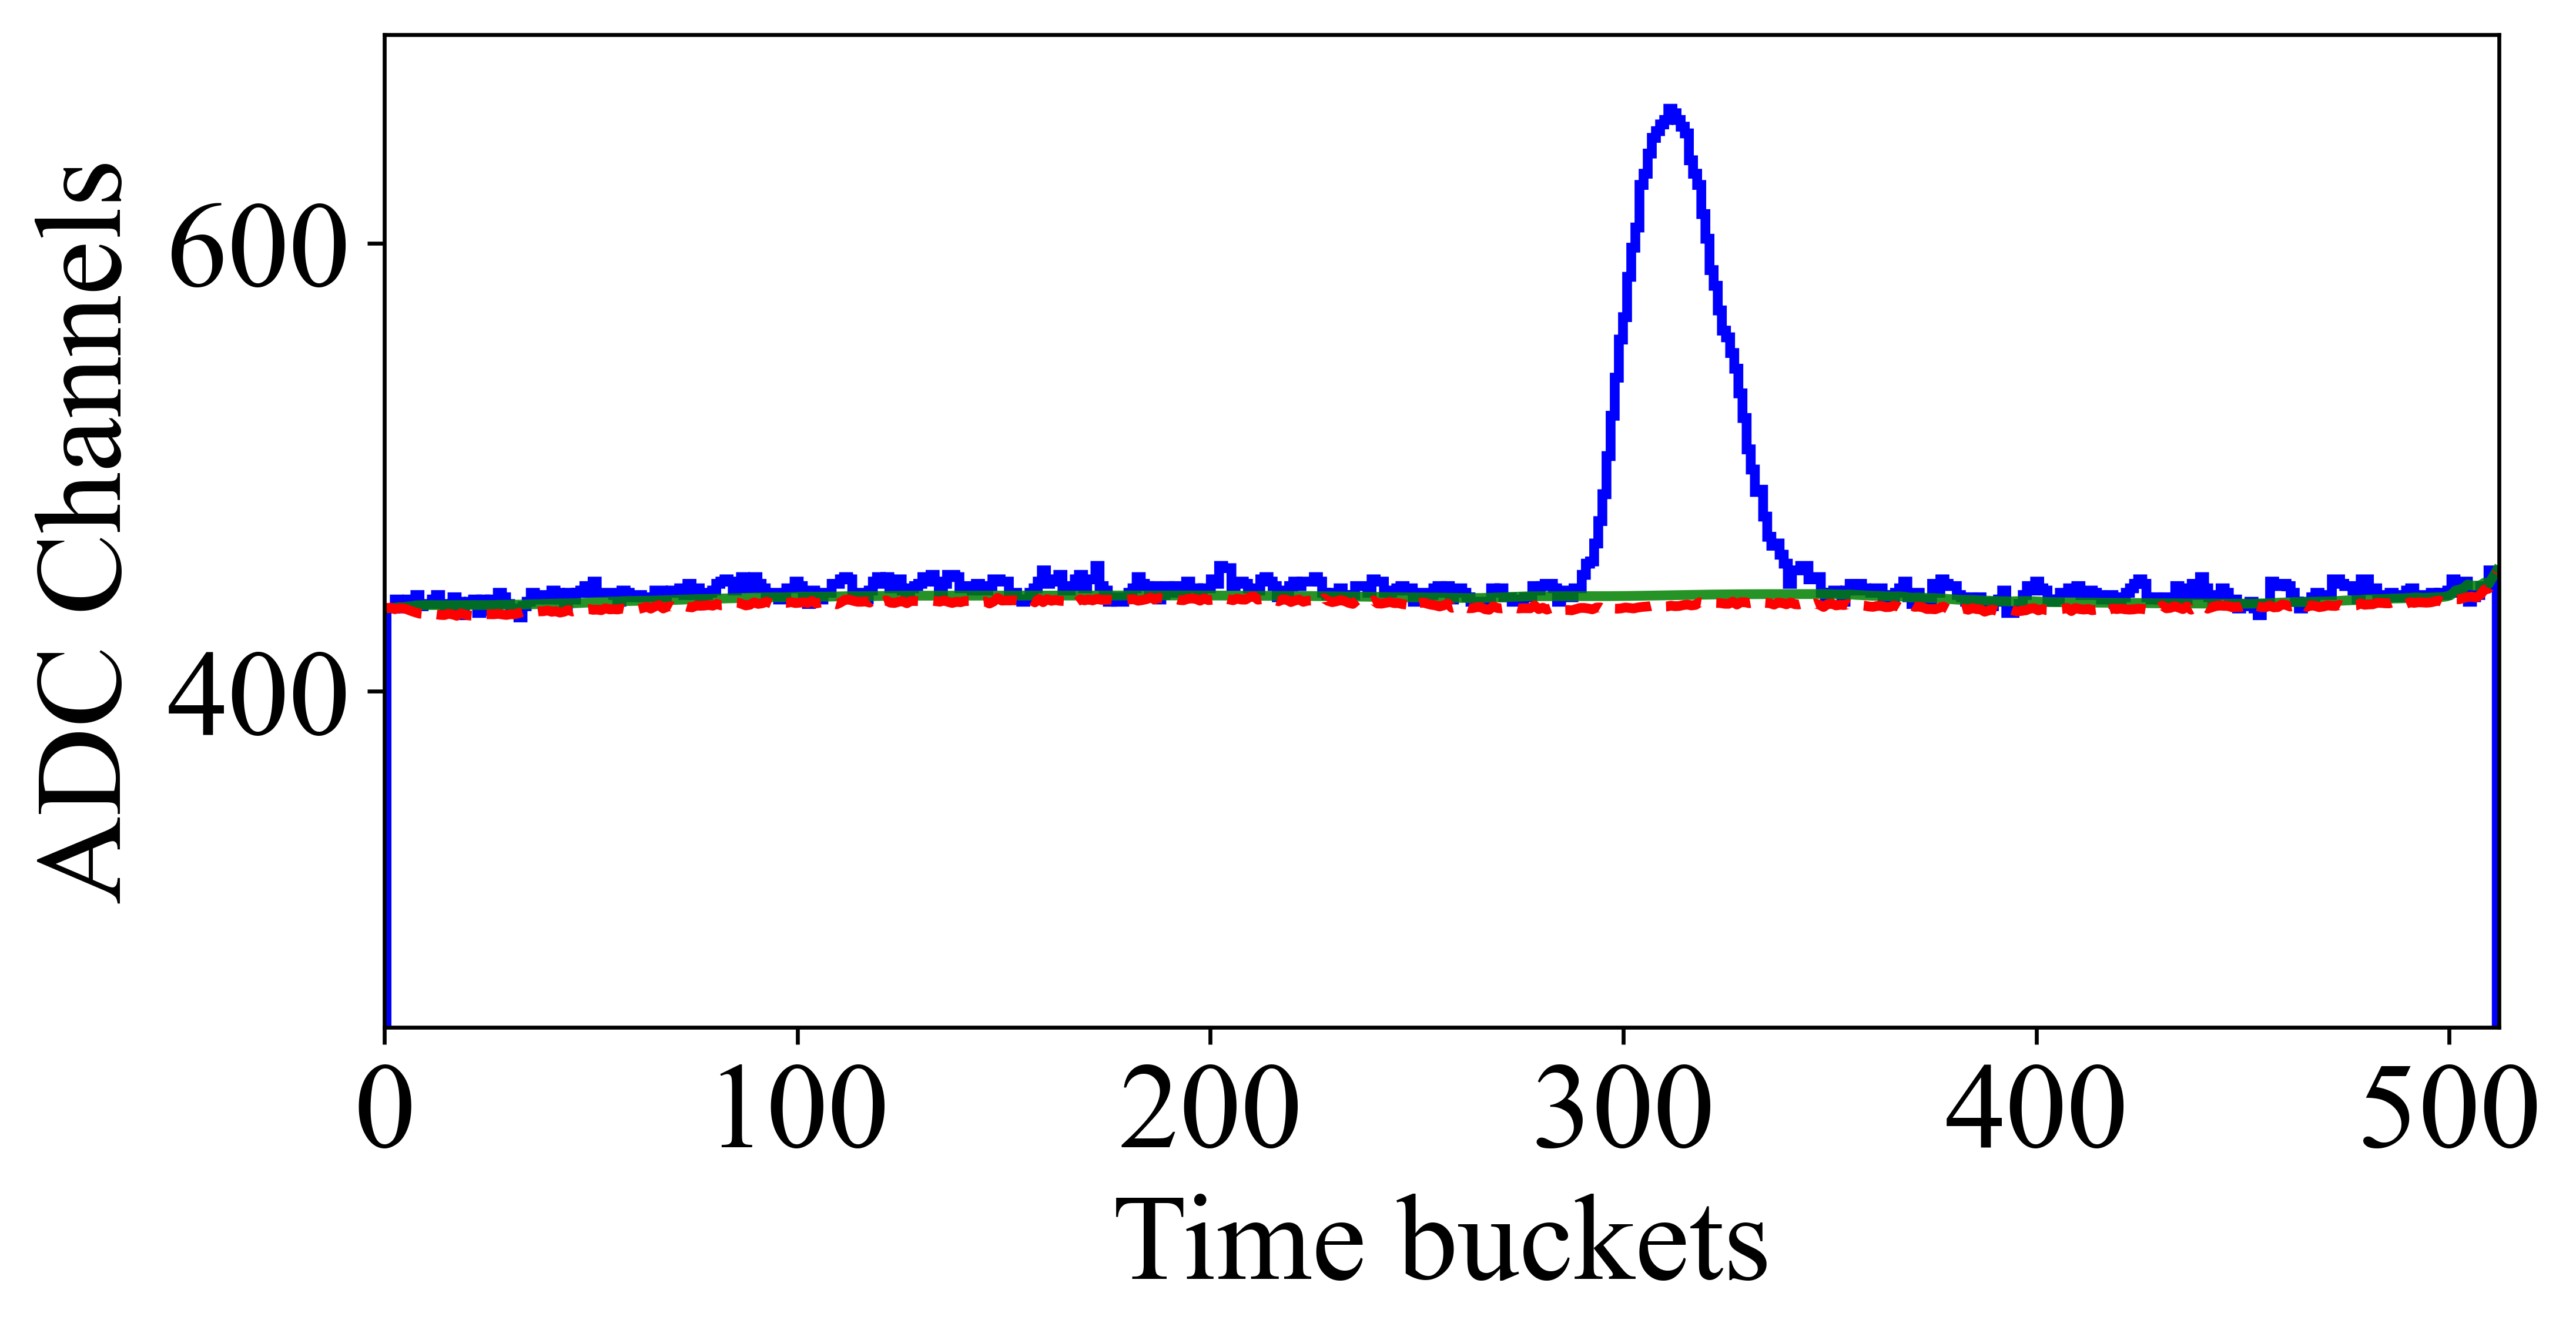
\includegraphics[scale=0.43]{figs/stb_3.png}
        \caption{}
        \label{subfig:stb_ex3}
    \end{subfigure}%
    \hfill
    \begin{subfigure}[b]{0.46\textwidth}
        \centering
        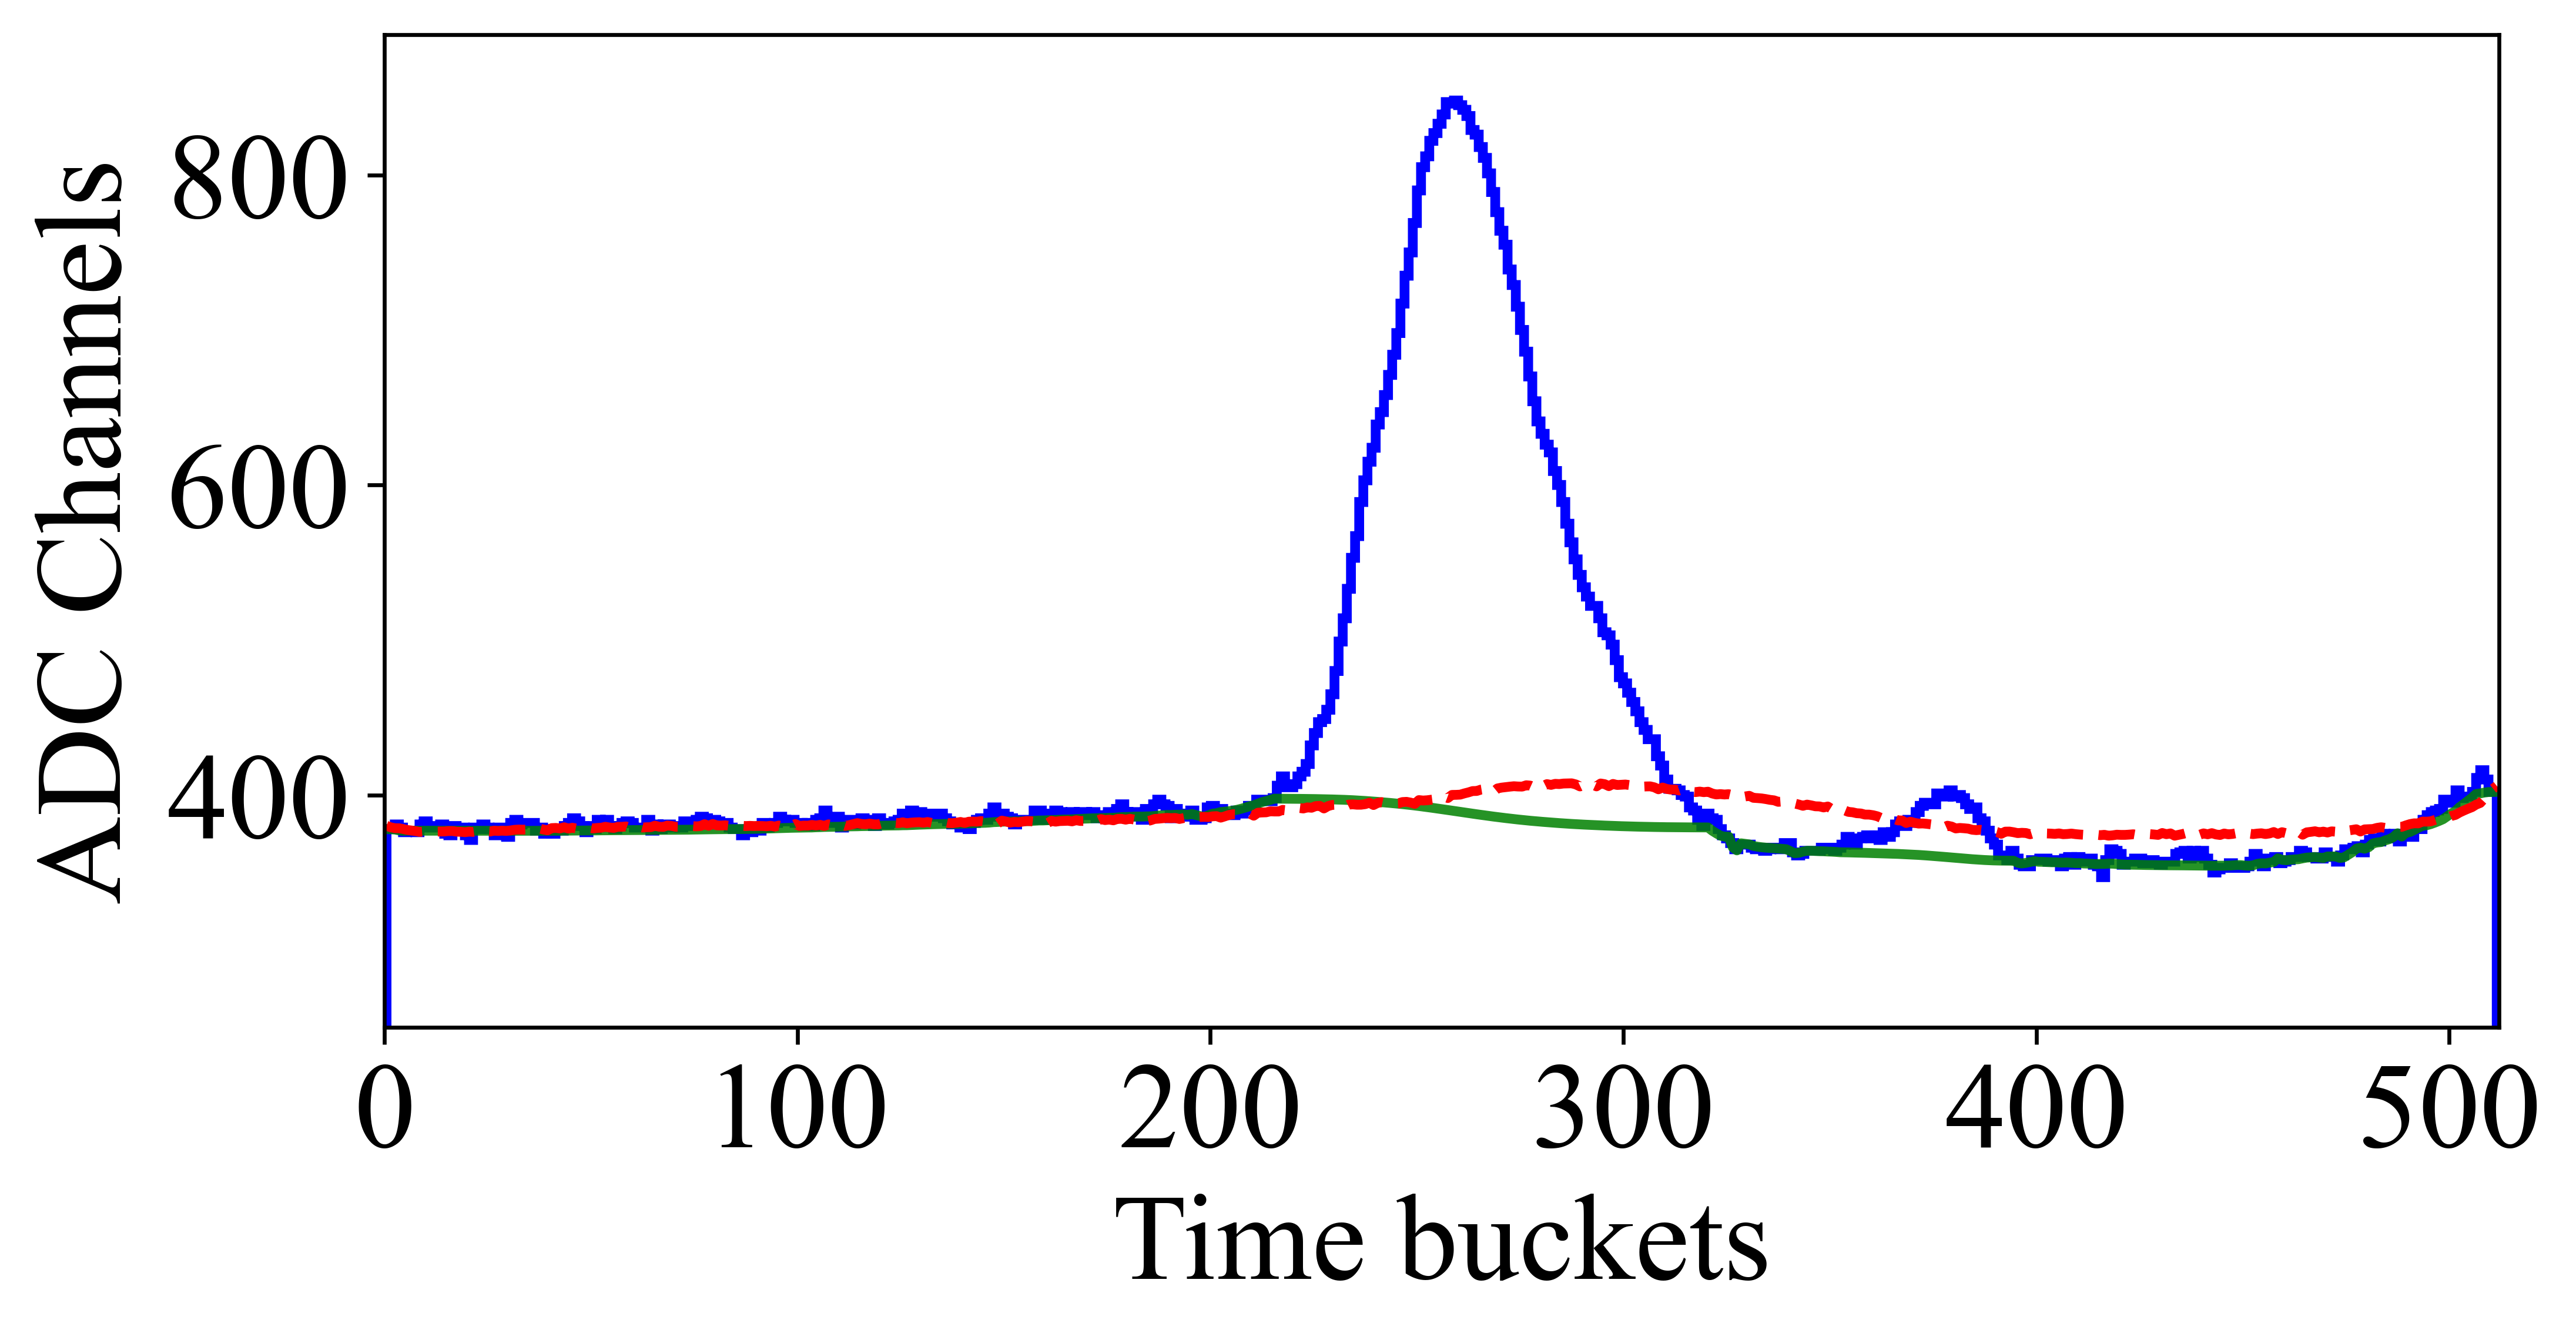
\includegraphics[scale=0.43]{figs/stb_4.png}
        \caption{}
        \label{subfig:stb_ex4}
    \end{subfigure}
\caption{Exemplos da rede neural dada pela figura \ref{fig:arq_source_to_bkg} em comparação com a saída do TSpectrum.}
\label{fig:stb_examples}
\end{figure}

\par Nos exemplos mostrados nas figuras \ref{subfig:stb_ex1}, \ref{subfig:stb_ex2} e \ref{subfig:stb_ex3} os fundos dos sinais possuem grande flutuação e a rede neural se mostrou eficaz na previsão. No exemplo \ref{subfig:stb_ex4} a baseline do sinal é relativamente complexa pois o sinal do canal 300 a 500, varia em cerca de 50 unidades em \textit{y}. Apesar da rede neural determinar o fundo, para esse caso, acima do fundo original, ao subtrair o espectro do fundo e colocar o valor mínimo em 0, o pulso presente entre os canais 200 e 300 é praticamente inalterado.

\par Com os resultados obtidos pela rede neural para a determinação do fundo, o próximo passo foi criar a rede neural que faz a deconvolução do espectro sem a baseline.

\subsection{Rede neural para a deconvolução}\label{subsec:pulso_ml_deconv}

% \par O próximo passo é construir uma rede neural que dê a posição dos picos. A tarefa a princípio não parece complicada. Pensando de forma simples, podemos fazer uma arquitetura curta e, como precisamos de uma saída de tamanho fixo, classificamos ponto a ponto como sendo não pico ou pico.

% \par O problema nessa abordagem é o desbalanço de classe evidente nos sinais. Caso tenhamos que classificar ponto a ponto em que, por exemplo, 0 representa um ponto que não é o centroide e 1 como um ponto que é um centroide, colocando na ultima camada a função de ativação \textit{sigmoid} (para sair valores entre 0 e 1), há muito mais valores 0 que 1. Se, por exemplo, temos um sinal que possui apenas um pico, teríamos que acertar o único valor 1 dentre 511 zeros. Caso a rede assuma que são 512 zeros, ainda assim a acurácia binária seria de mais de 99\%.

% \par Outro problema é que há um \textit{overlap} de gaussianas. Não é tão evidente a posição dos centroides se o espectro não está deconvoluído. É muito mais complicado, mesmo olhando, dizer a posição. Portanto o problema será quebrado em mais uma etapa: construir um rede que faça a deconvolução.

\par Considerando a mesma abordagem da rede neural anterior criamos uma rede neural para realizar uma sequencia de convoluções e por fim uma camada \textit{fully connected} com função de ativação ReLU, pois precisamos ter o valor mínimo do espectro em 0, assim como a saída do algoritmo de deconvolução do TSpectrum. Os filtros das convoluções precisam ter tamanho mínimo de duas vezes o sigma das gaussianas utilizadas para atuarem sobre cada pulso do espectro. A entrada da rede é o sinal já com o fundo subtraído e com mínimo em 0. A saída é o sinal após deconvolução dada pelo algoritmo \textsc{gold deconvolution} na biblioteca TSpectrum do ROOT, já mostrado na subseção \ref{subsec:pulses_deconv}. A figura \ref{fig:source_to_deconv} mostra a arquitetura da rede de deconvolução. A rede é a sequência de duas convoluções com 32 filtros (passagens \textit{a} e \textit{b}), \textit{valid padding} e filtros de tamanho 19 e 17, respectivamente. Sem o \textit{valid padding}, nós temos a saída com tamanho reduzido, como o da segunda arquitetura mostrada na figura \ref{fig:source_to_deconv} (como o tamanho do filtro é 19, não é possível aplicar a convolução em 9 pontos em cada extremidade, então, o sinal resultante tem tamanho $494=512-18$). O \textit{valid padding} se mostrou mais eficiente para a convergência da rede. Toda a rede foi construída usando o TensorFlow 2, possuindo 508.000 parâmetros treináveis \cite{FORTINO2022166497}.


% seguida de uma camada \textit{Max pooling} com \textit{pool size} igual à 16. No final há o flat na camada para seguir com uma camada fully connected com função de ativação ReLU. O valid padding se mostrou mais eficiente para a convergência da rede. Toda a rede foi construída usando o TensorFlow 2, possuindo 508.000 parâmetros treináveis \cite{FORTINO2022166497}.

\par Assim como na rede anterior, foram usados 160.000 sinais para treino e 40.000 para validação. O \textit{loss} foi escolhido como sendo o erro quadrático médio, o otimizador foi o ADAM, com \textit{learning rate} de 0.0005 porém com o parâmetro \textit{clipnorm} igual a 0.45 que serve para alterar a norma do vetor gradiente da função do custo. Isso significa que, caso a norma do vetor do gradiente exceda 0.45, então o valor da norma é reajustado para o limiar (\textit{threshold}) escolhido (0.45) \cite{FORTINO2022166497}. Isso faz com que não ocorra problemas comuns como o gradiente sumir \cite{VGP, ADAMAX}, um dos problemas que teve que ser resolvido nessa rede. A métrica para avaliação foi o erro médio absoluto. Foram 75 \textit{epochs} e o \textit{batch-size} foi 8. Os resultados do treino estão na figura \ref{fig:source_wo_bkg_to_deconv_results}.

%\par Alterar a norma do vetor gradiente da função custo (usar o parâmetro clipnorm = 0.45) significa que, caso a norma do vetor do gradiente exceda 0.45, então o valor da norma é reajustado para o limiar (threshold) escolhido (0.45) \cite{FORTINO2022166497}. Isso faz com que não ocorra problemas comuns como o gradiente sumir \cite{VGP, ADAMAX}, um dos problemas que teve que ser resolvido nessa rede.

\par O treino foi realizado no Google Colaboratory \cite{google_colab} usando a GPU NVIDIA Tesla P100 e demorou cerca de 54 minutos. Os resultados do treino estão na figura \ref{fig:source_to_bkg_results}, onde eles indicam que, visualmente, a rede neural consegue distinguir muito bem diferentes centróides presentes no pulso. Empiricamente, a rede é capaz de executar 200.000 sinais em 5.4 segundos (ou 37.000 sinais por segundo).

\begin{figure}[H]
    \centering
    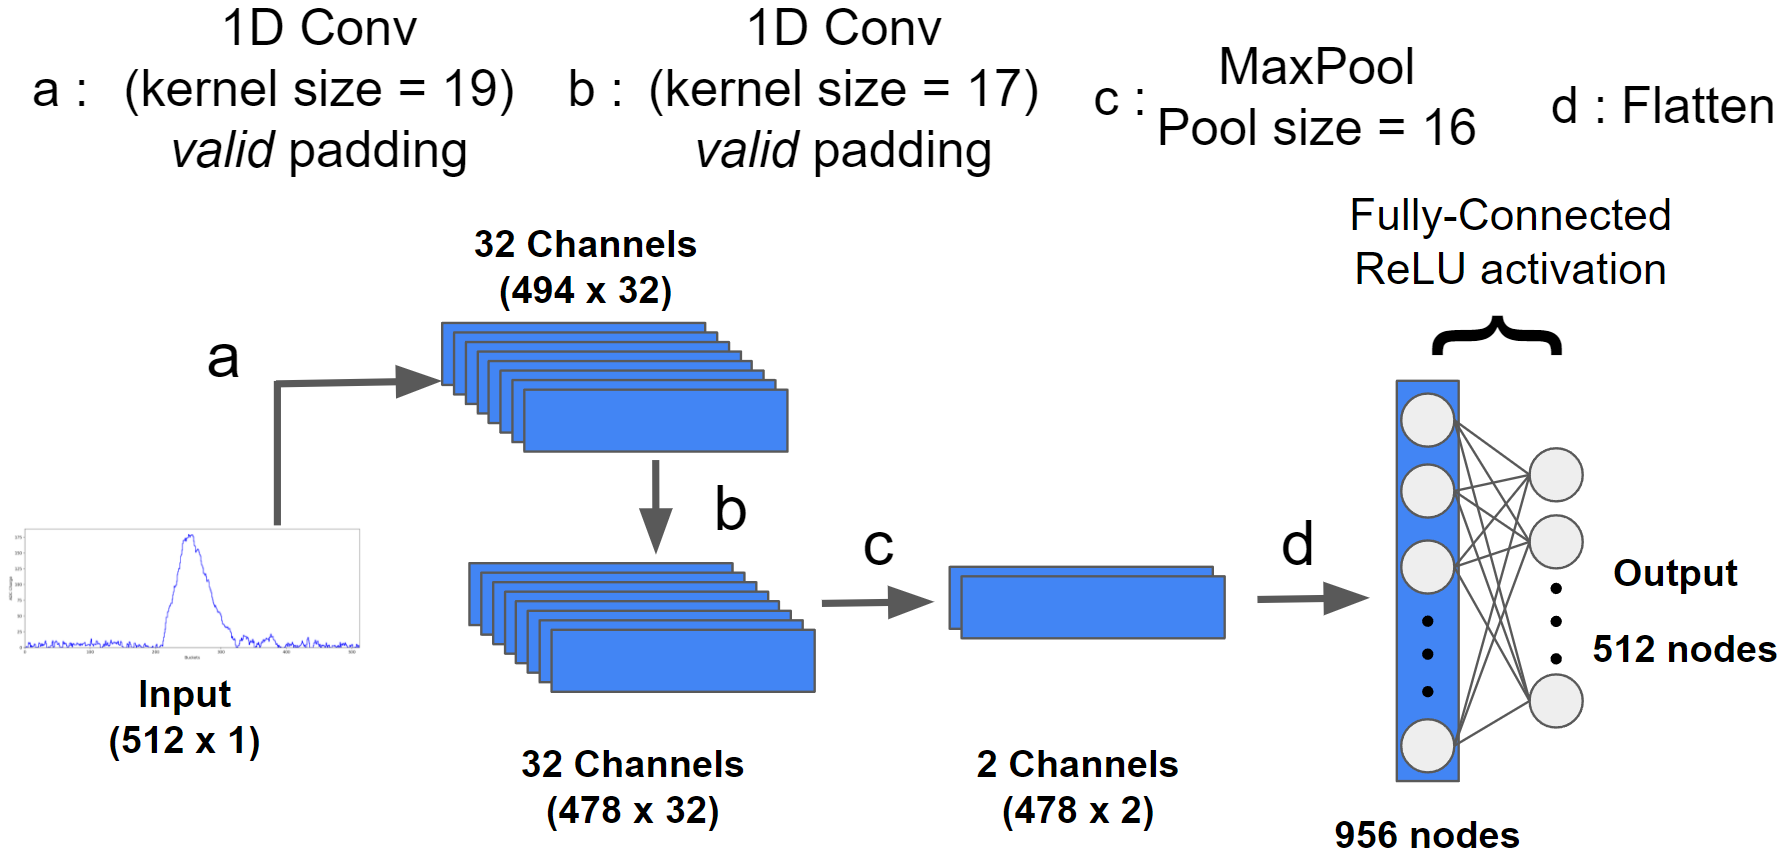
\includegraphics[scale = 0.28]{figs/source_wobkg_to_deconv.png}
    \caption{Arquitetura da rede neural que faz a inferência da deconvolução do espectro. O vetor de entrada deve ter dimensionalidade 512 x 1. Todas as partes com convolução não possuem o parâmetro bias.}
    \label{fig:source_to_deconv}
\end{figure}

\begin{figure}[H]
\centering
    \begin{subfigure}[t]{0.49\textwidth}
        \centering
        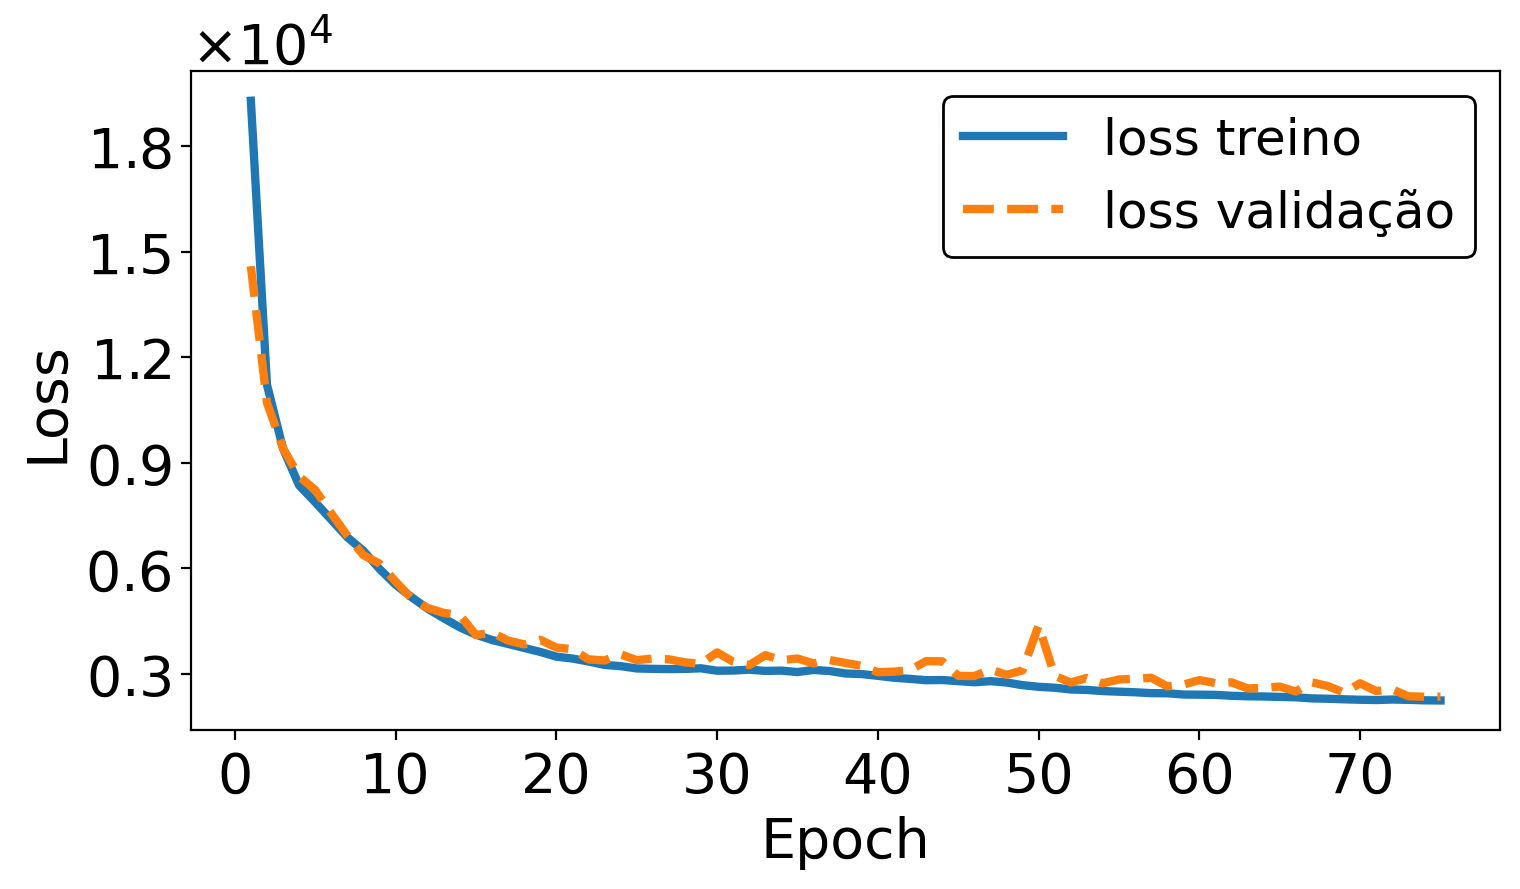
\includegraphics[scale=0.42]{figs/source_wo_bkg_to_deconv_loss.png}
        \caption{Loss dos dados de treino (linha contínua) e dos dados de validação (linha tracejada) em função da epoch no treino da rede dada pela figura \ref{fig:source_to_deconv}.}
        \label{subfig:source_wo_bkg_to_deconv_loss}
    \end{subfigure}%
    \hfill
    \begin{subfigure}[t]{0.465\textwidth}
        \centering
        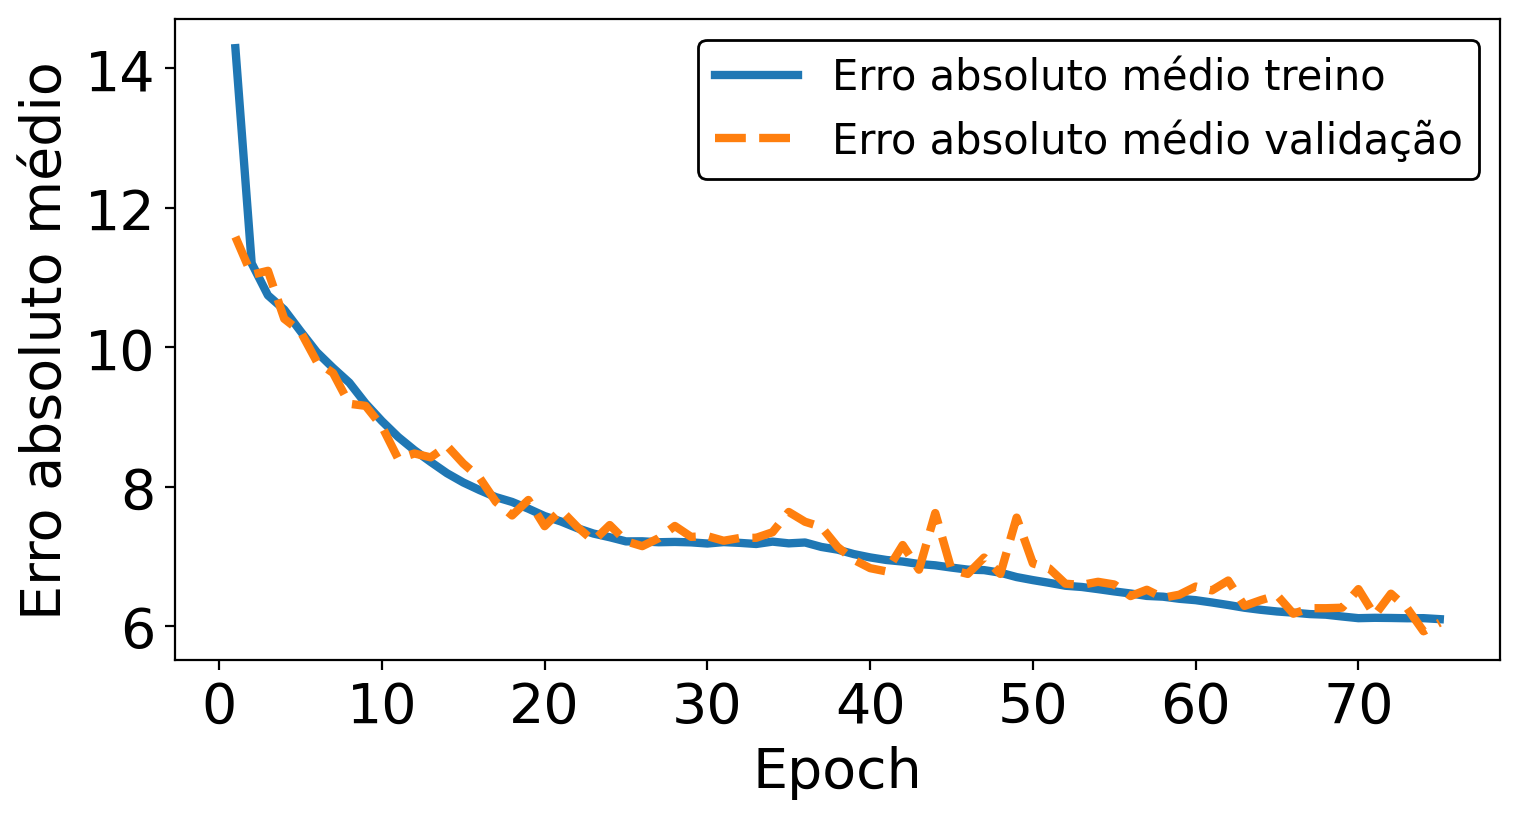
\includegraphics[scale=0.42]{figs/source_wo_bkg_to_deconv_metric.png}
        \caption{Erro absoluto médio dos dados de treino (linha contínua) e dos dados de validação (linha tracejada) em função da epoch no treino da rede dada pela figura \ref{fig:source_to_deconv}.}
        \label{subfig:source_wo_bkg_to_deconv_metric}
    \end{subfigure}
\caption{Resultados do treino da rede neural dada pela figura \ref{fig:arq_source_to_bkg}.}
\label{fig:source_wo_bkg_to_deconv_results}
\end{figure}

% \par A mudança em relação à rede que faz a inferência do sinal de fundo é que o \textit{padding} das camadas agora é \textit{valid}. Agora não estamos verificando pontos onde seriam necessários adicionar zeros além do vetor de entrada, como explicado na seção \ref{sec:ml}. O \textit{padding} \textit{valid} se mostrou mais eficiente com relação à separação das gaussianas, dando melhor resolução para buscar os centroides. Além disso, ao colocar o \textit{pool size} de apenas 16, para poder dar um \textit{flat} na camada seguinte, fez com que a resolução de separação das gaussianas fosse inclusive melhor que a do algoritmo analítico. A figura \ref{fig:std_examples} mostra um exemplo da saída da rede.

\begin{figure}[H]
\centering
    \begin{subfigure}[b]{0.49\textwidth}
        \centering
        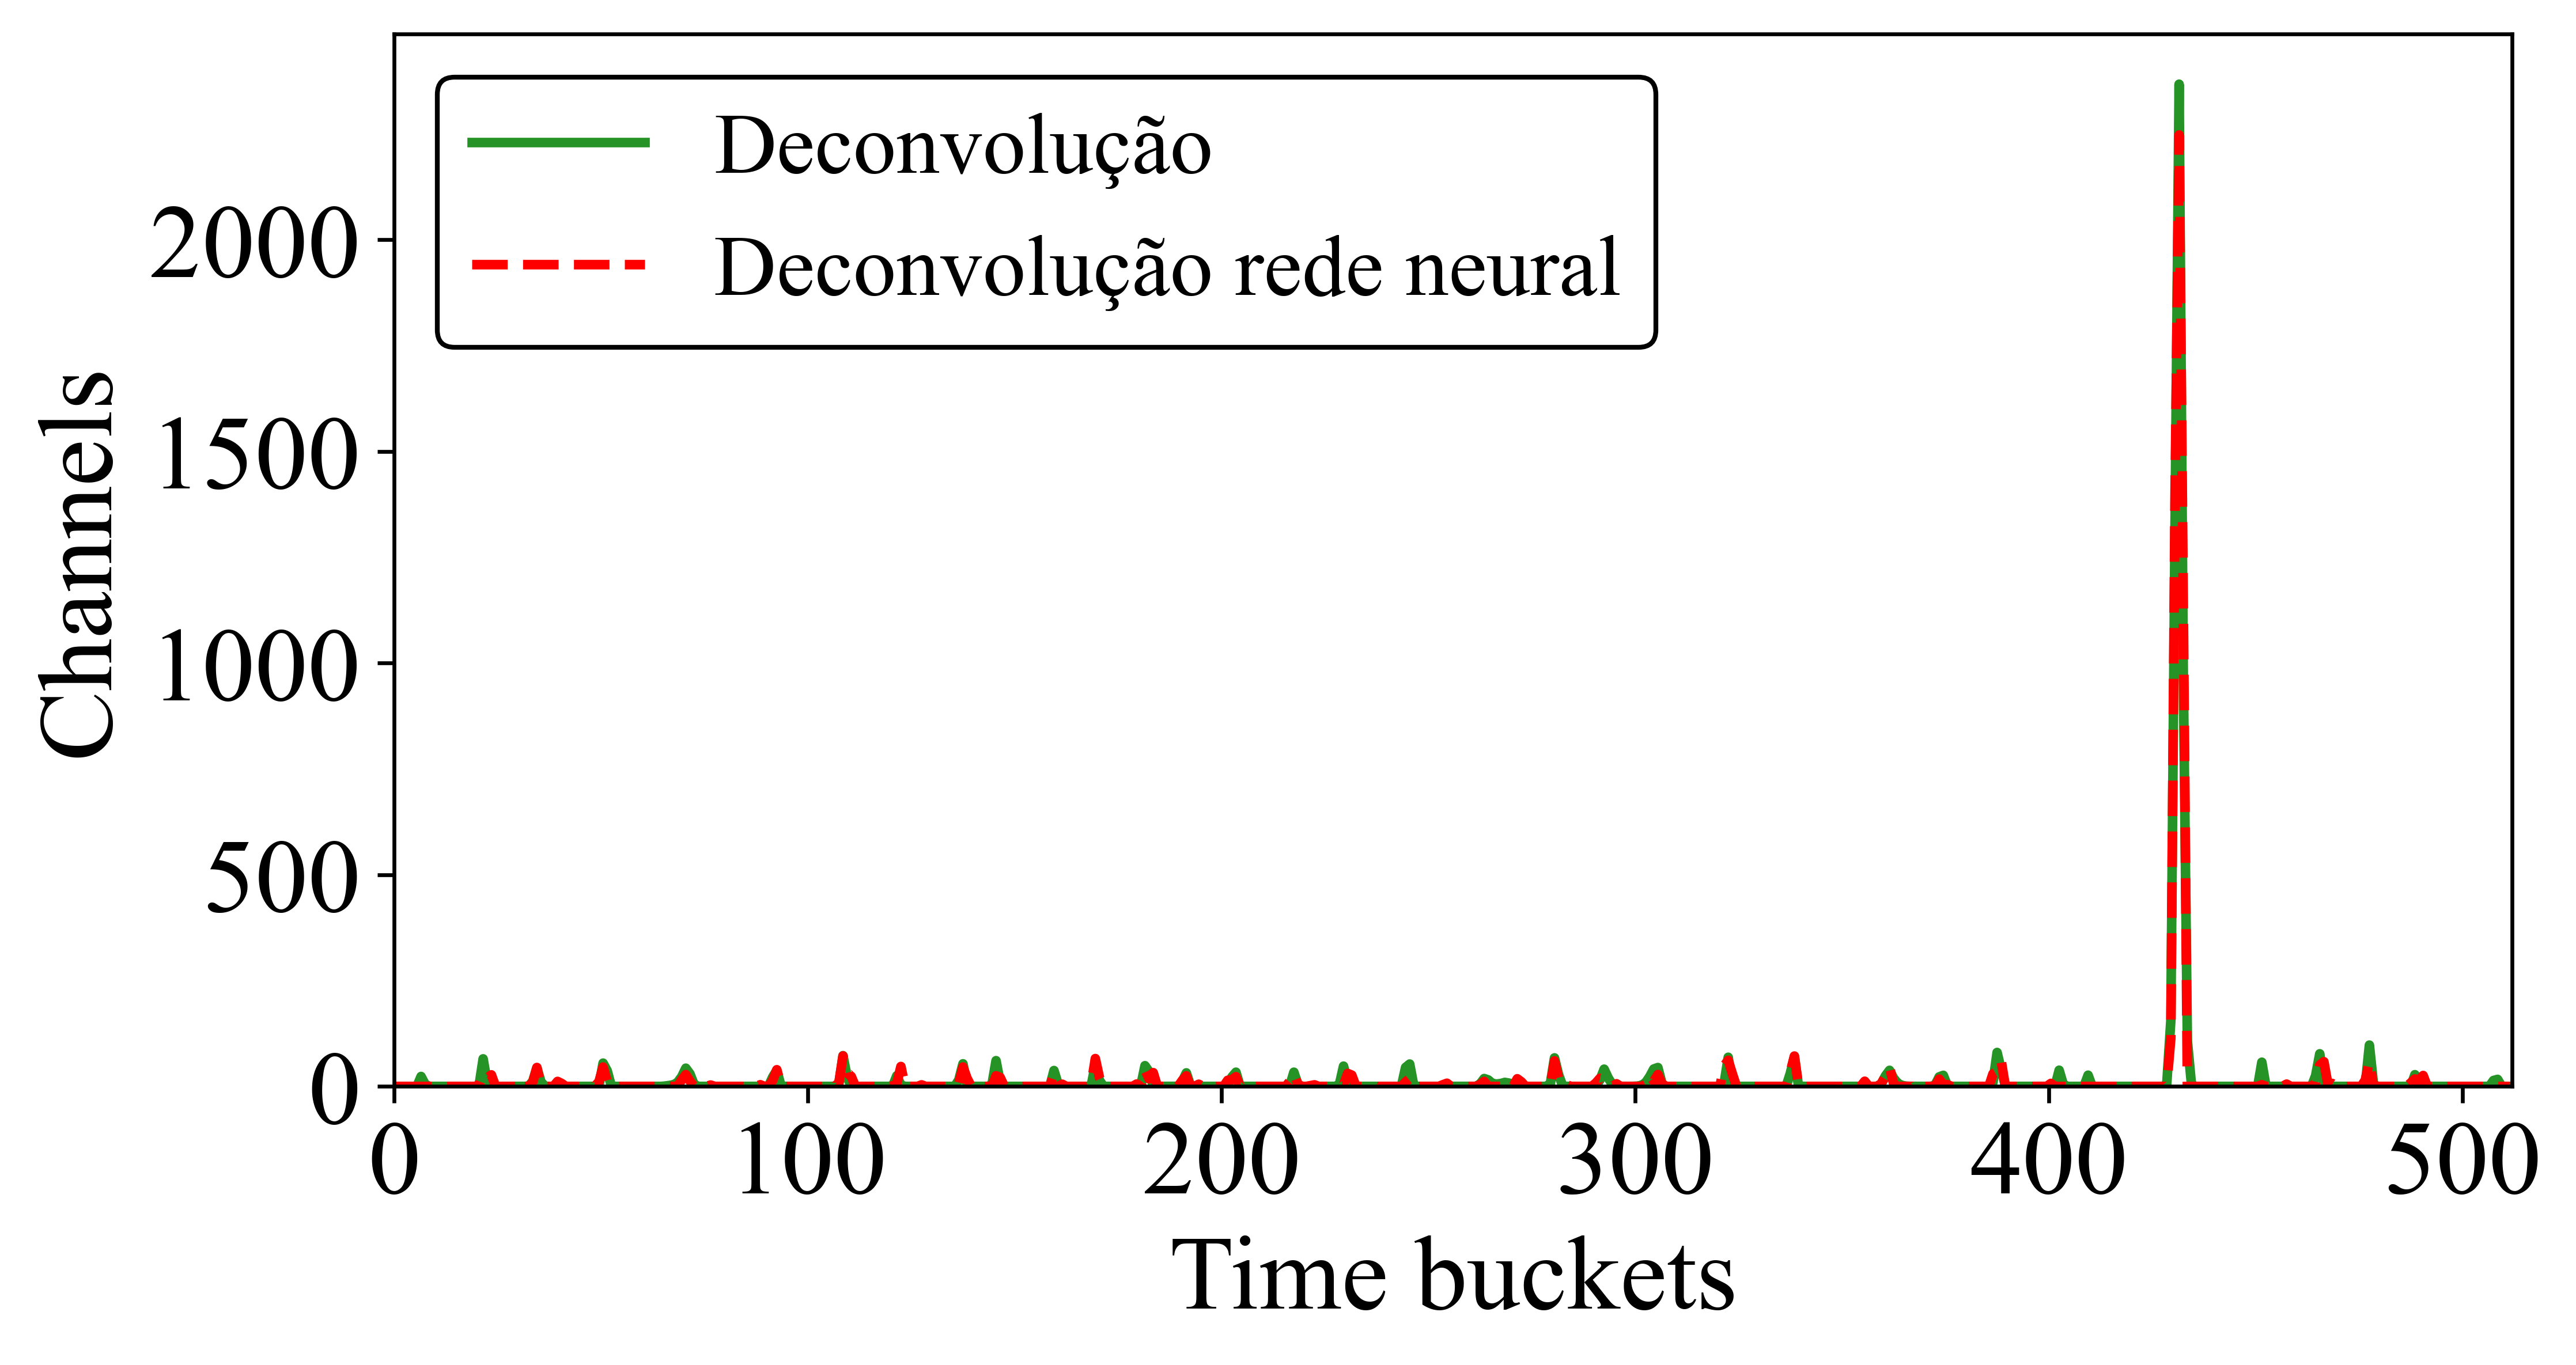
\includegraphics[scale=0.425]{figs/swbtd_1.png}
        \caption{}
        \label{subfig:std_ex1}
    \end{subfigure}%
    \hfill
    \begin{subfigure}[b]{0.465\textwidth}
        \centering
        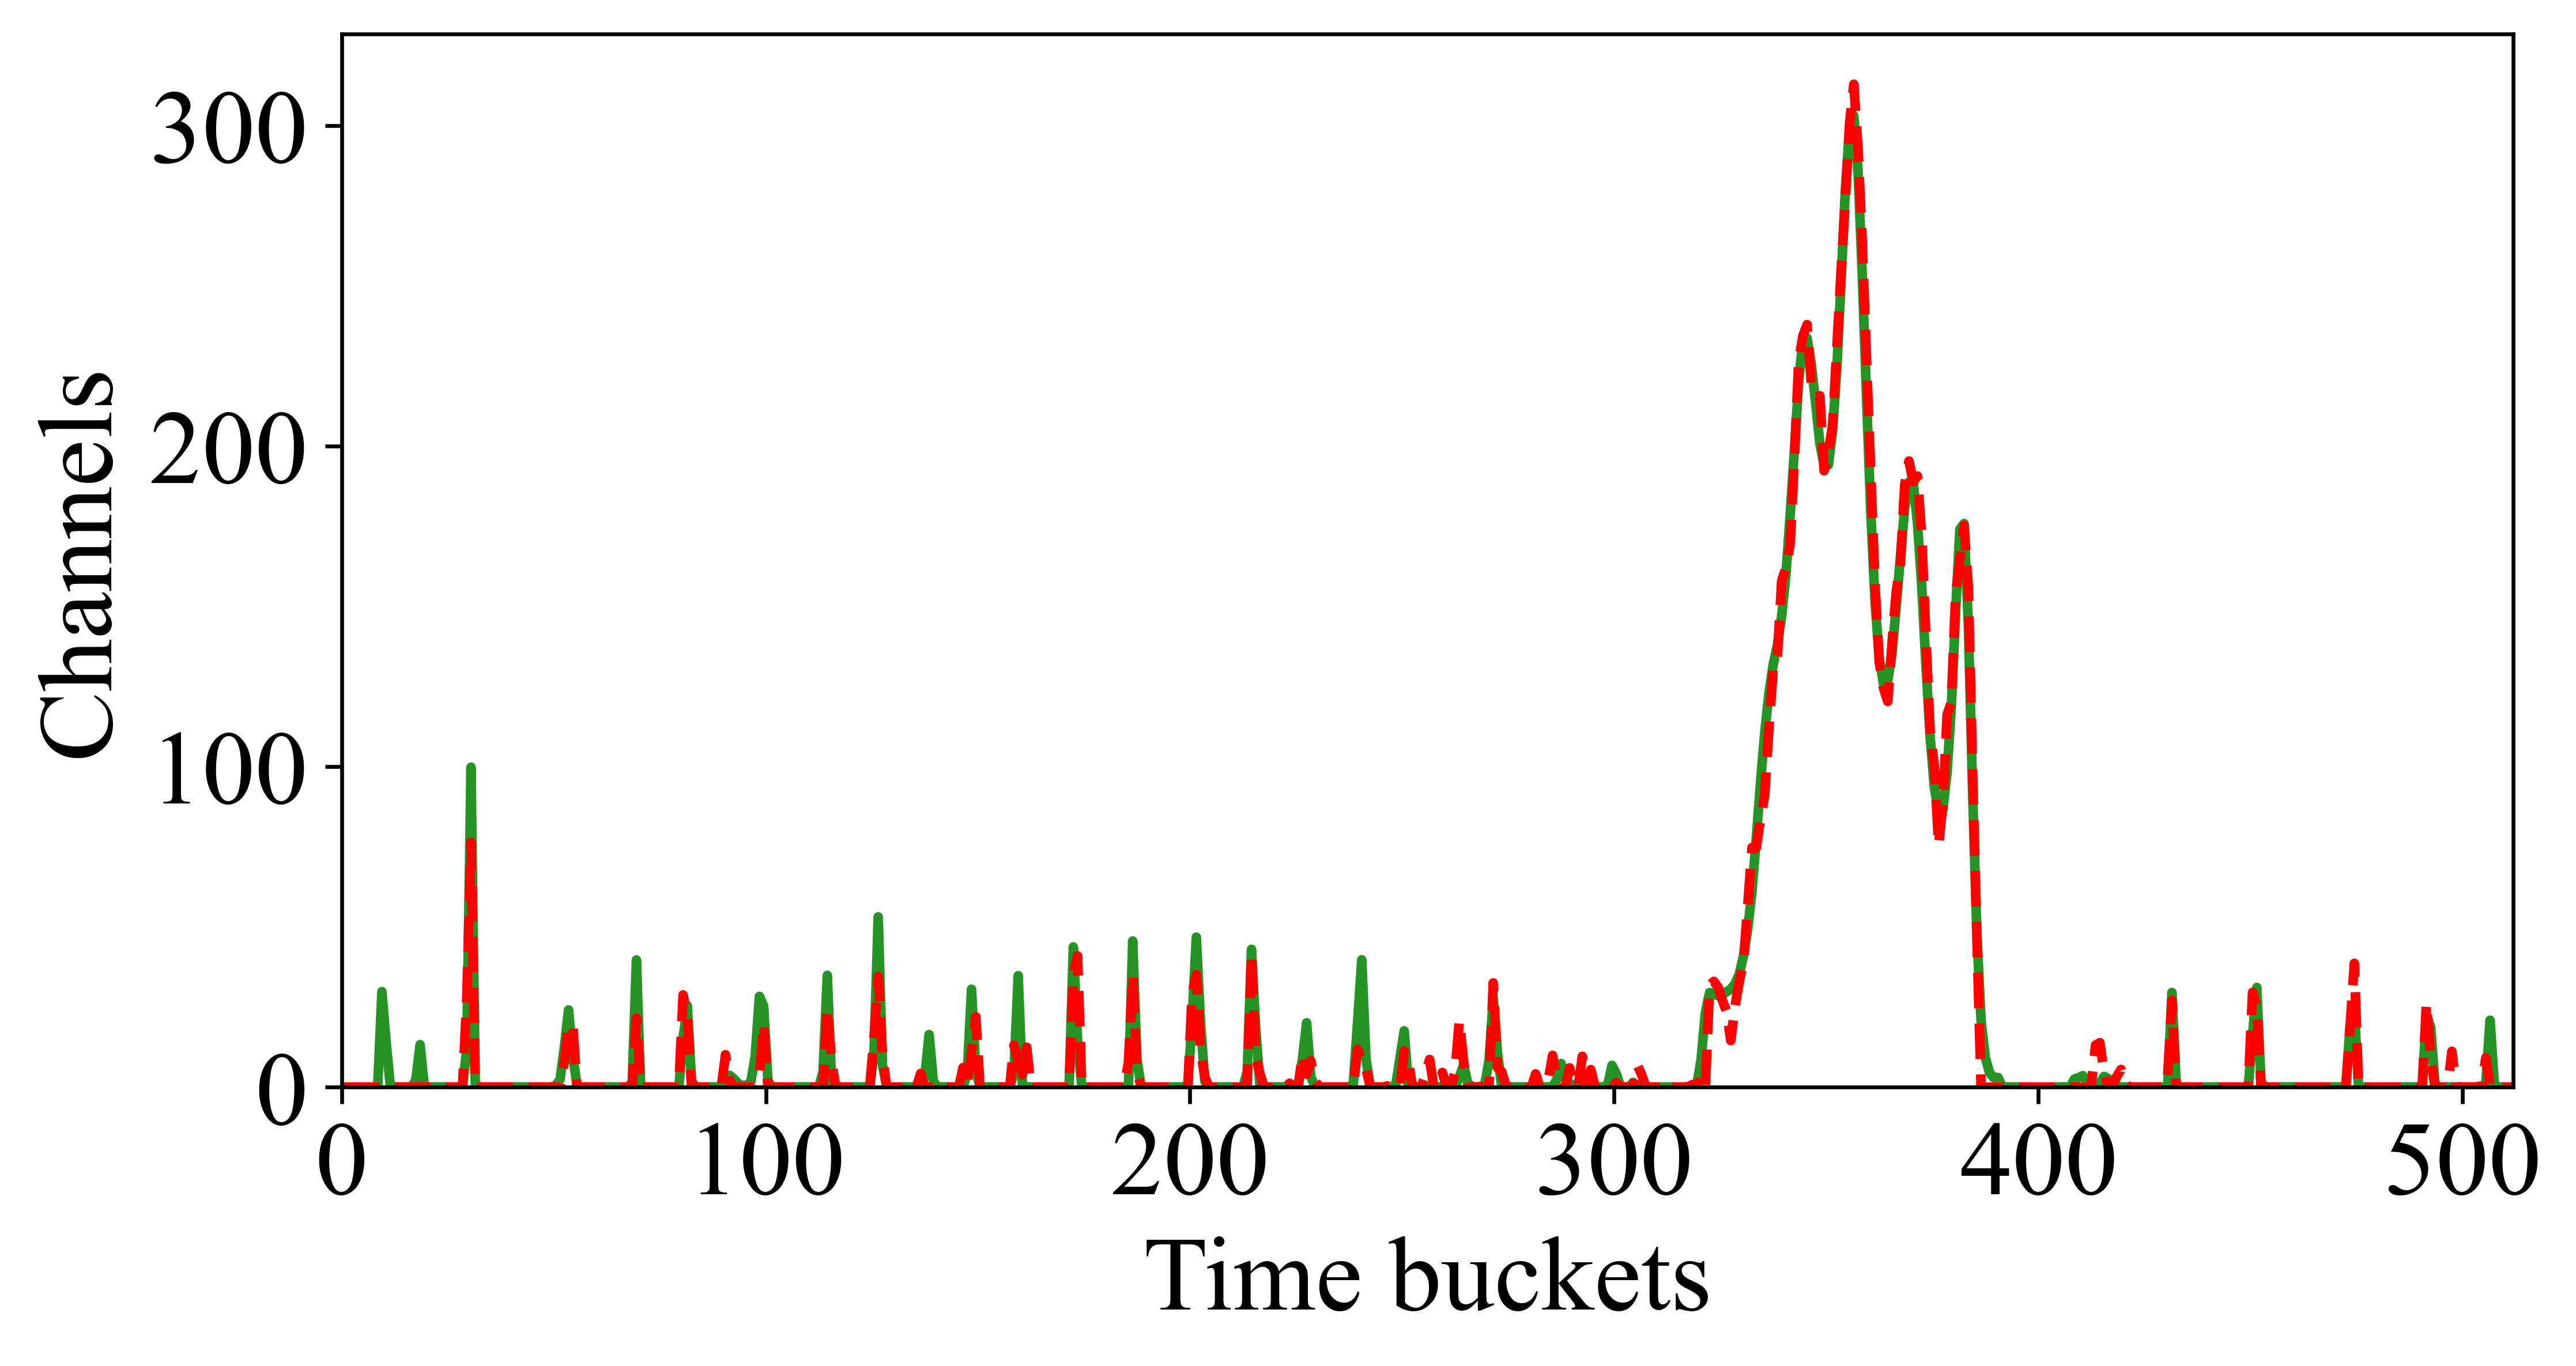
\includegraphics[scale=0.425]{figs/swbtd_2.png}
        \caption{}
        \label{subfig:std_ex2}
    \end{subfigure}
    \begin{subfigure}[b]{0.49\textwidth}
        \centering
        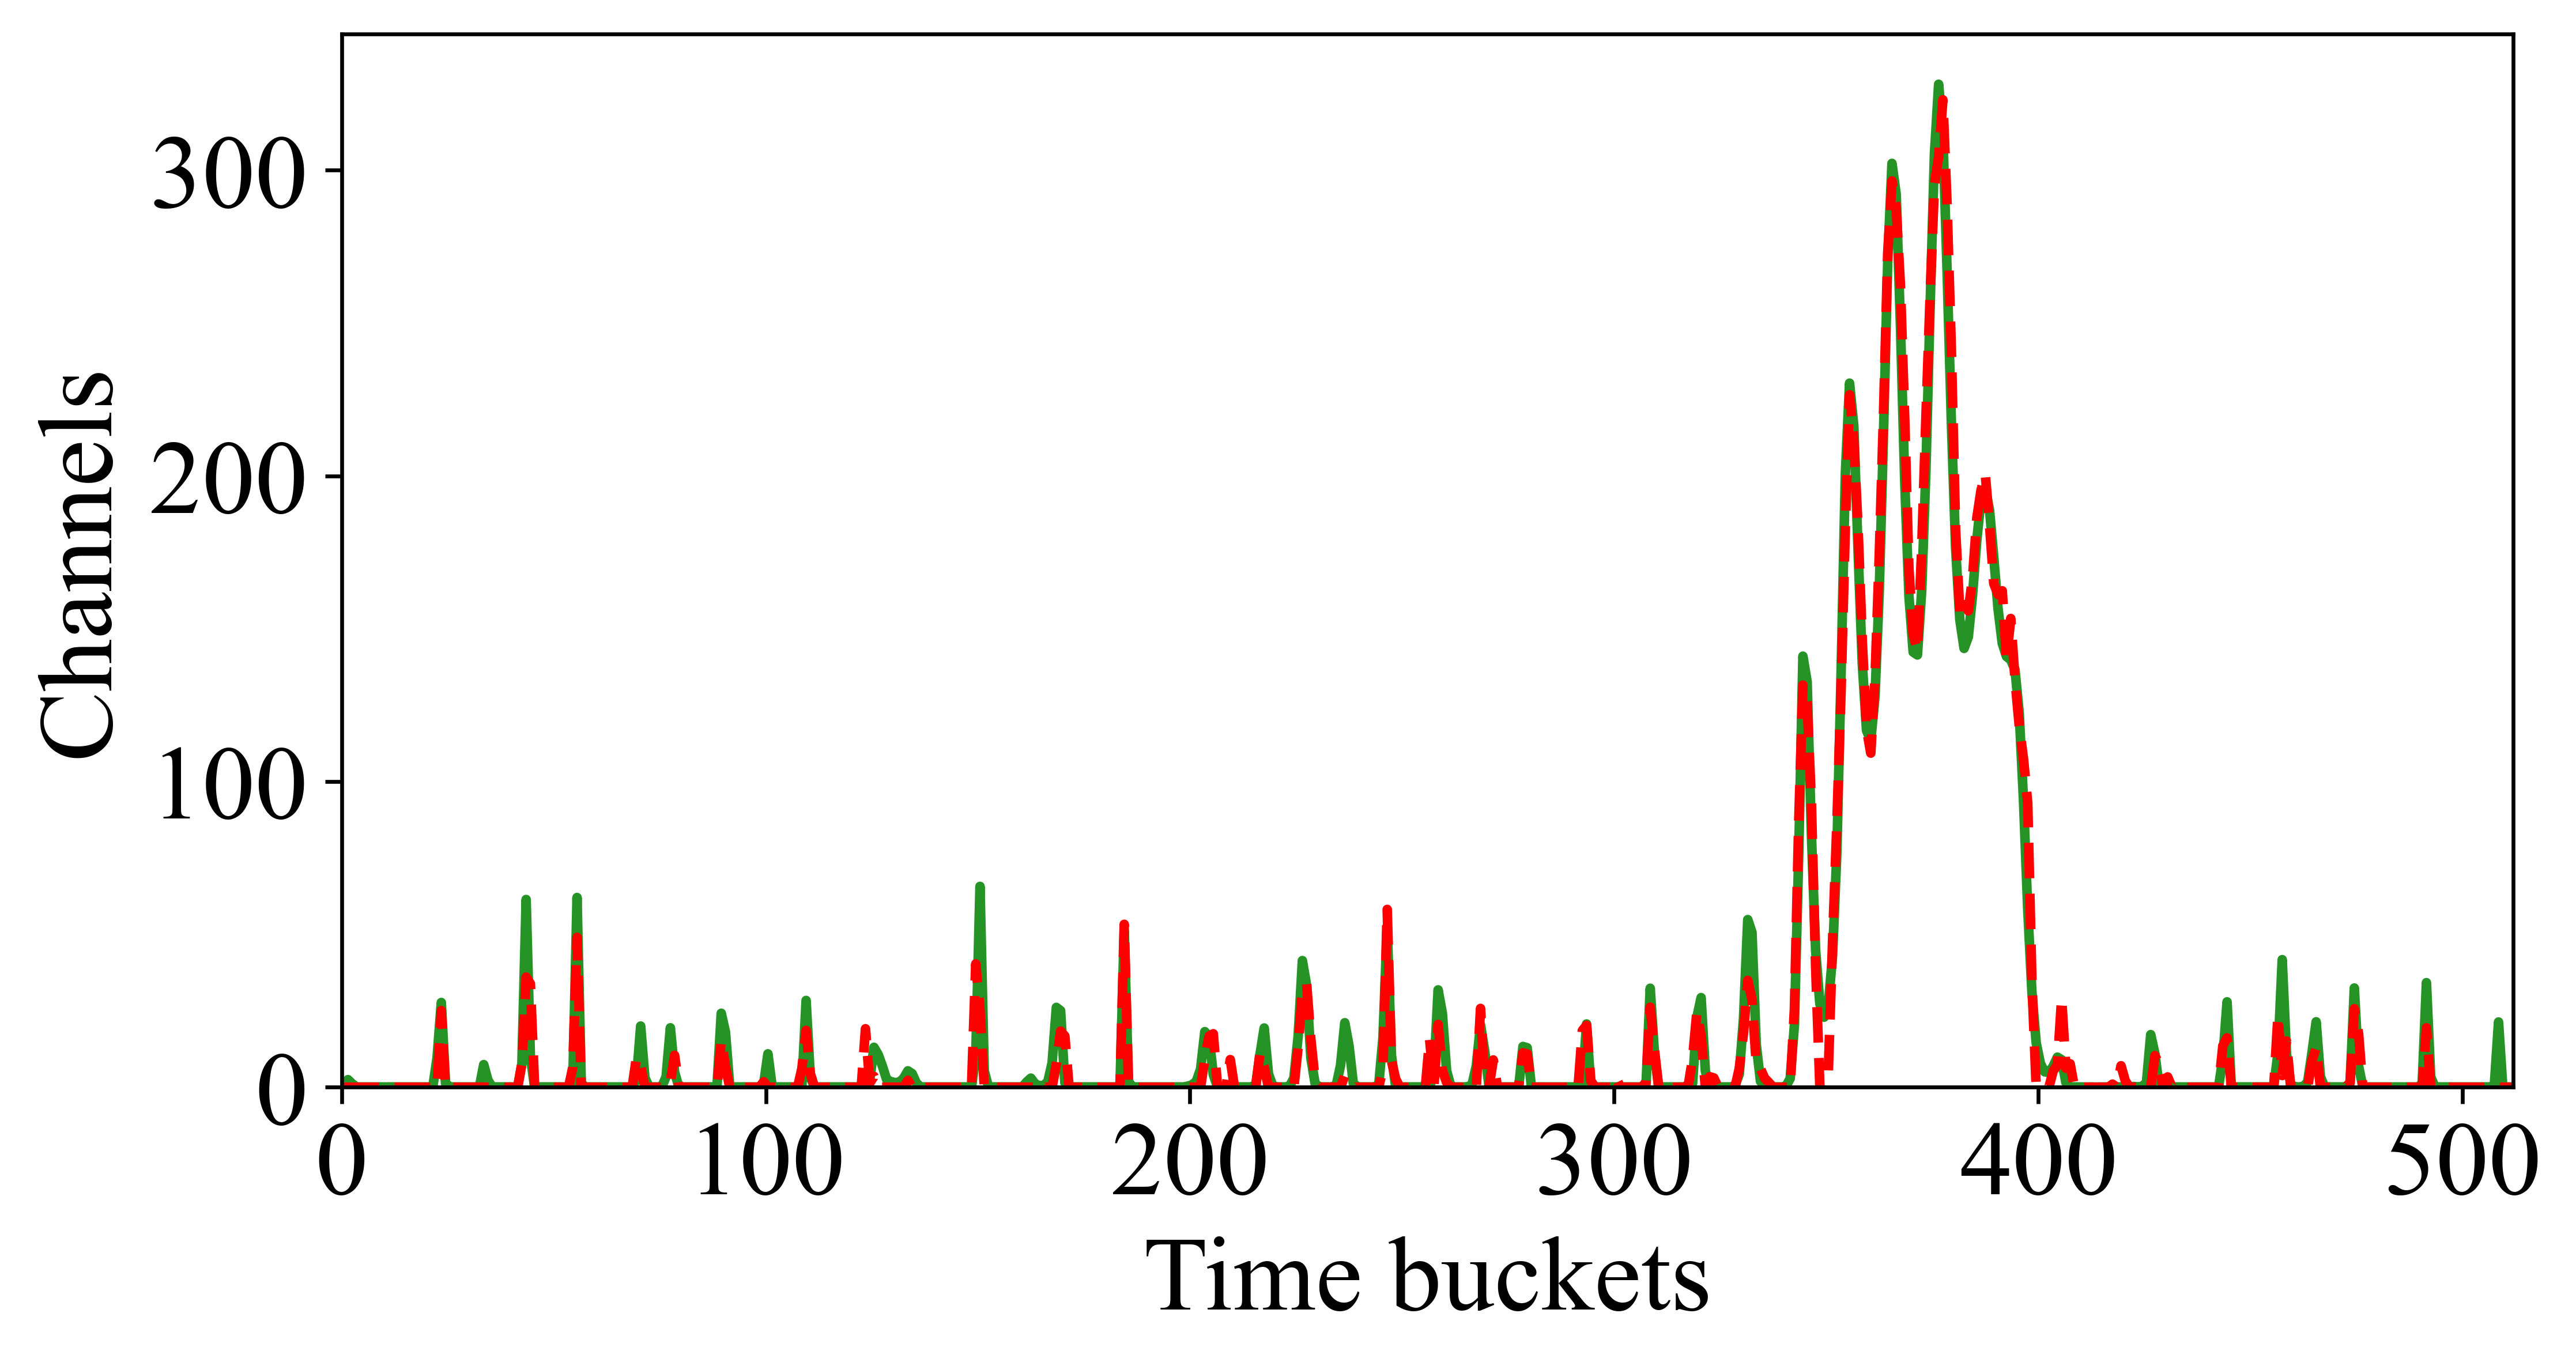
\includegraphics[scale=0.425]{figs/swbtd_3.png}
        \caption{}
        \label{subfig:std_ex3}
    \end{subfigure}%
    \hfill
    \begin{subfigure}[b]{0.465\textwidth}
        \centering
        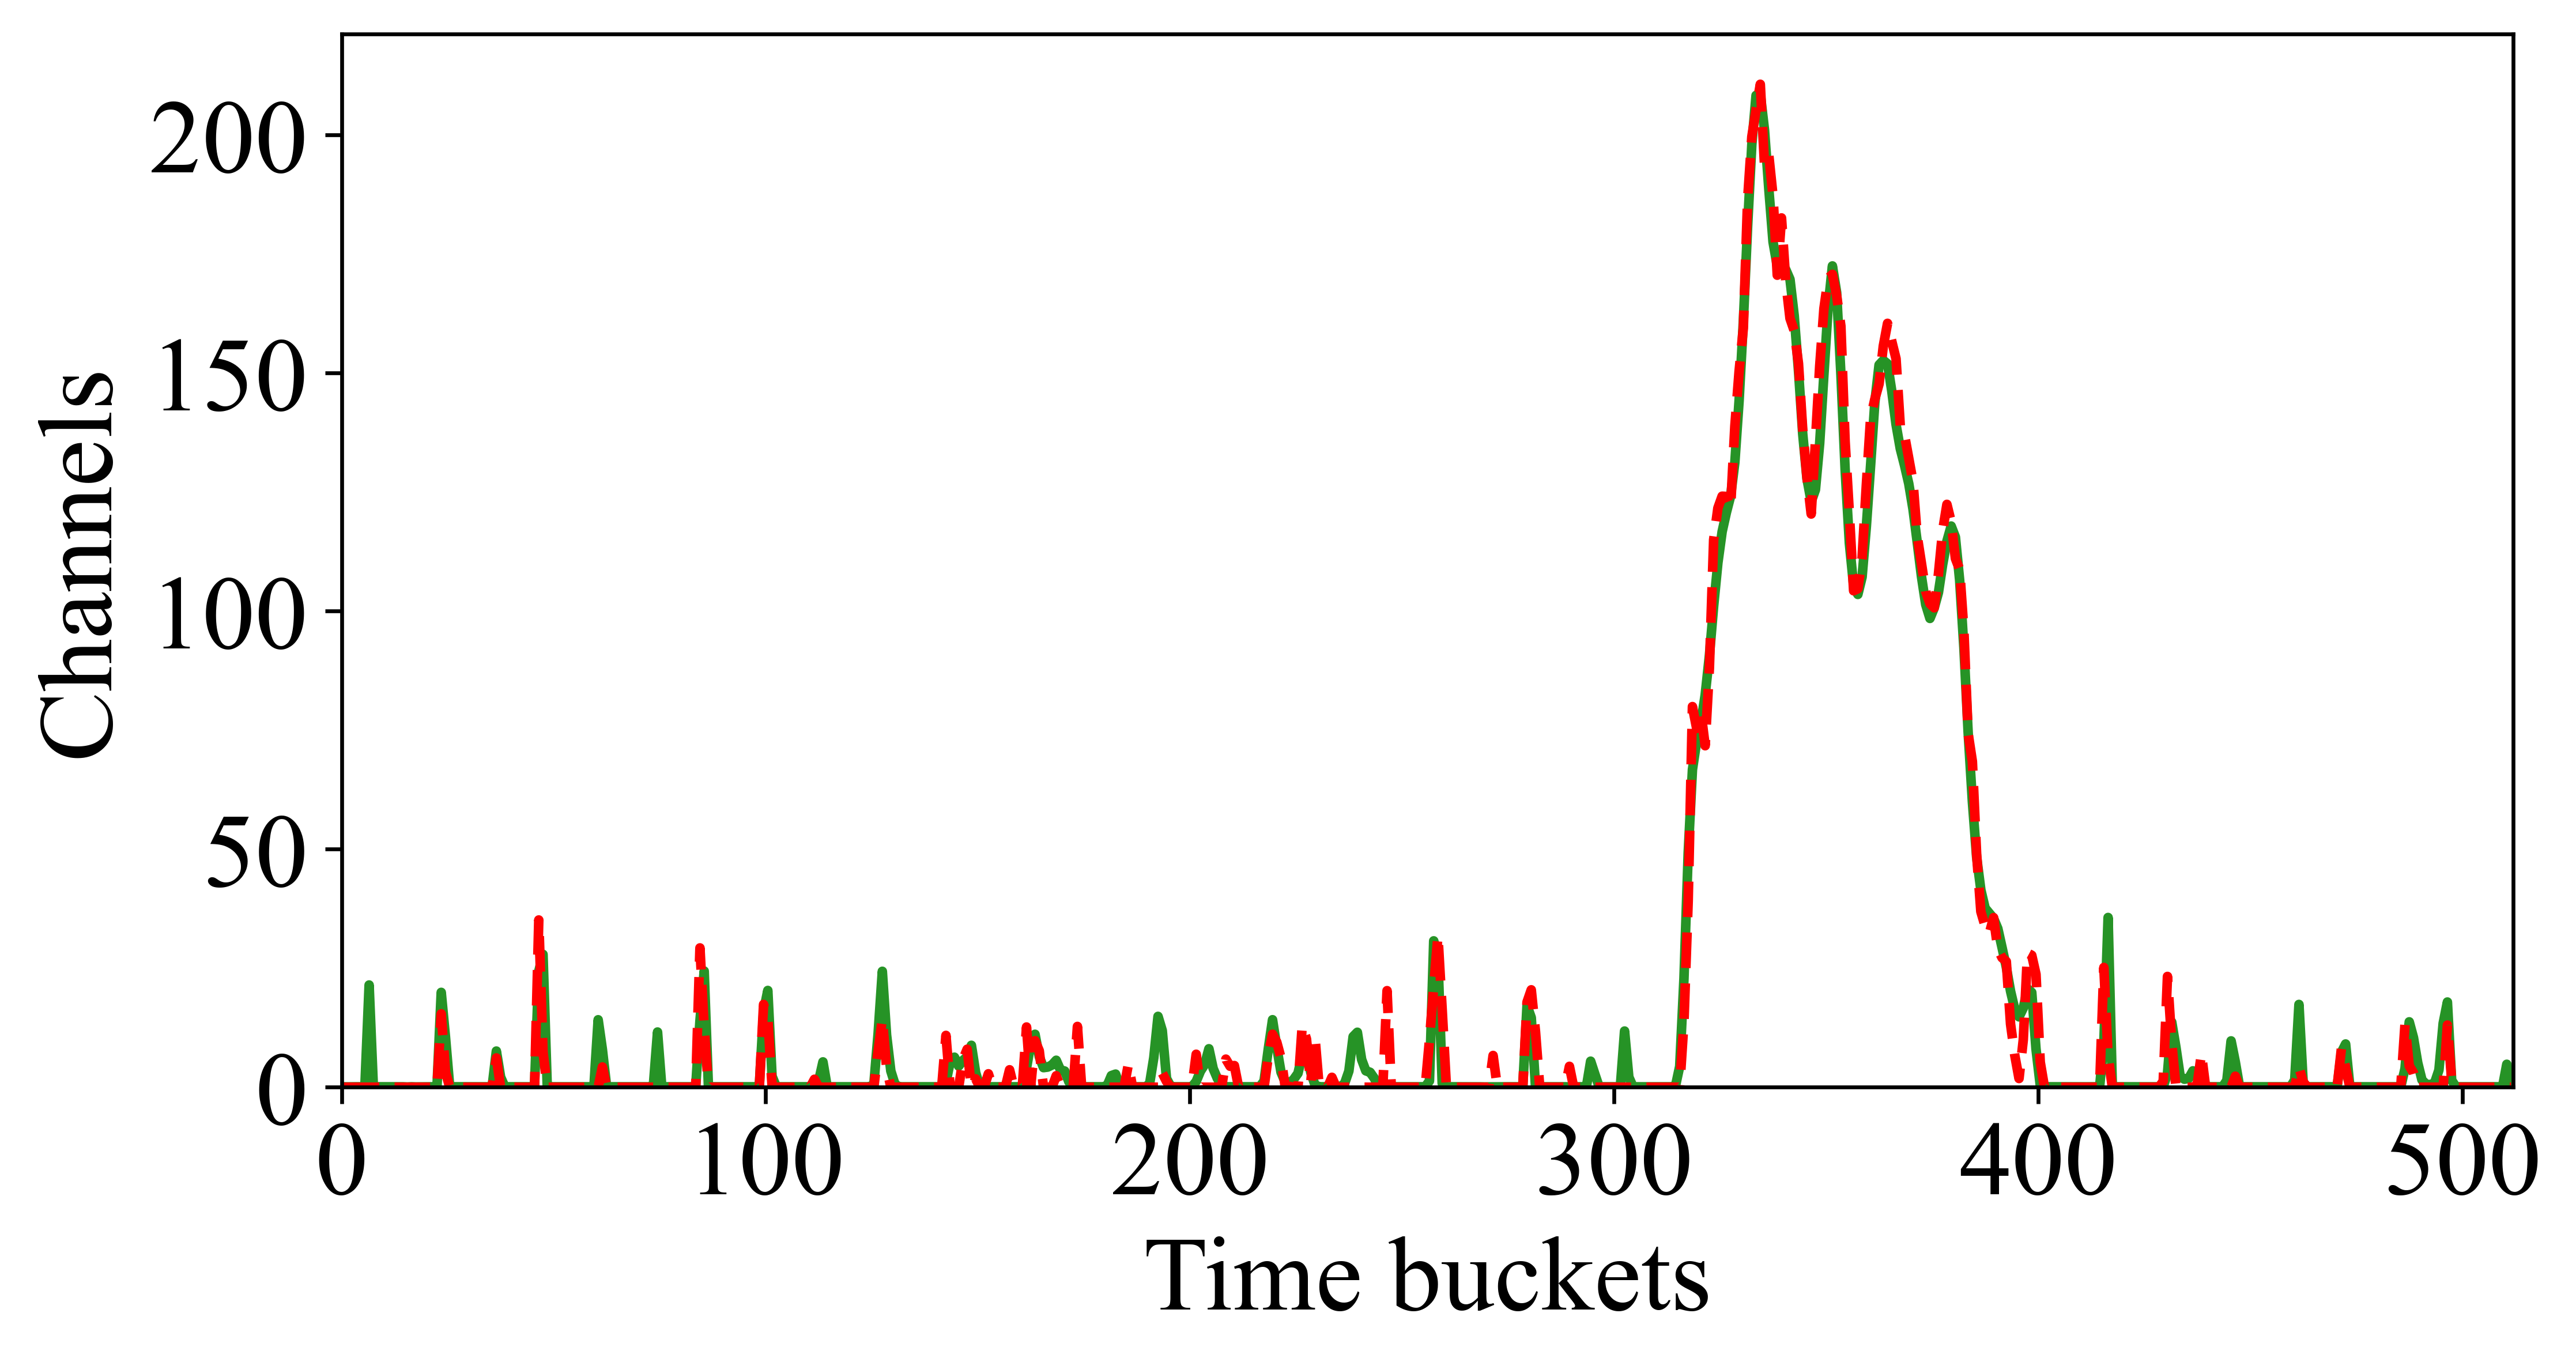
\includegraphics[scale=0.425]{figs/swbtd_4.png}
        \caption{}
        \label{subfig:std_ex4}
    \end{subfigure}
\caption{Exemplos de deconvolução da rede neural dada pela figura \ref{fig:arq_source_to_bkg}.}
\label{fig:std_examples}
\end{figure}

\par Com a rede neural para a deconvolução determinada e funcionando, a última etapa é a construção de uma rede neural para a identificação de picos, mostrada na \ref{subsec:pulso_ml_peaks}.

\subsection{Identificação de picos}\label{subsec:pulso_ml_peaks}

\par A última etapa dessa análise com machine learning foi analisar e determinar uma solução para a identificação de picos. A identificação dos picos se tornou um desafio complexo, pois há uma variação muito grande na quantidade de picos por sinal e também há um desbalanço muito grande na quantidade de pontos comuns (aqueles que não são picos) e pontos que são picos. Por exemplo, caso haja um sinal que possui apenas um pico, deve-se identificar uma posição, gerar um valor de saída como 1. Por exemplo, para 512 pontos, um \textit{time bucket} deve ter o valor 1 e os outros 511 terão o valor de saída como 0. Caso a rede determine que todos os pontos não são picos, ainda assim a acurácia binária seria maior que 99\%. Isso é conhecido como desbalanço de classe \cite{inproceedings}.

\par Para corrigir esse desbalanço, foram acrescentados pontos simetricamente em torno do pulso, de forma que a somatória das amplitudes das regiões é equivalente a carga $Q$ acumulada no ponto. Isso faz com que não seja preciso identificar um único ponto, mas sim uma região em torno do pico. Com isso podemos nos basear na ideia de segmentar o sinal para destacar regiões de interesse \cite{aly2011research}. Segmentar significa ter uma rede neural com a saída com o mesmo tamanho do vetor de entrada (512) e saída com valores entre 0 e 1, onde 1 indica uma região com um pico e 0 não. A figura \ref{fig:n_peaks_exs} mostra um exemplo de um sinal após a deconvolução onde picos foram identificados com o algoritmo \textsc{peak\_finder} e os pontos foram acrescentados simetricamente em torno dos picos para representar as regiões dos pulsos.

% \par Para resolver esse problema podemos nos basear na ideia de recortar regiões de interesse, como feito pela rede U-Net\cite{unet}. Recortar regiões significa, nesse caso, ter uma rede neural com a saída com o mesmo tamanho do vetor de entrada (512) e saída com valores entre 0 e 1, onde 1 indica uma região com um pico e 0 não. Como temos as posições dos picos, basta acrescentar pontos simetricamente em torno do pulso. A figura \ref{fig:n_peaks_exs} mostra um exemplo de um sinal após a deconvolução onde há o pico detectado e os pontos acrescentados para representar a região do pulso.

\begin{figure}[H]
    \centering
    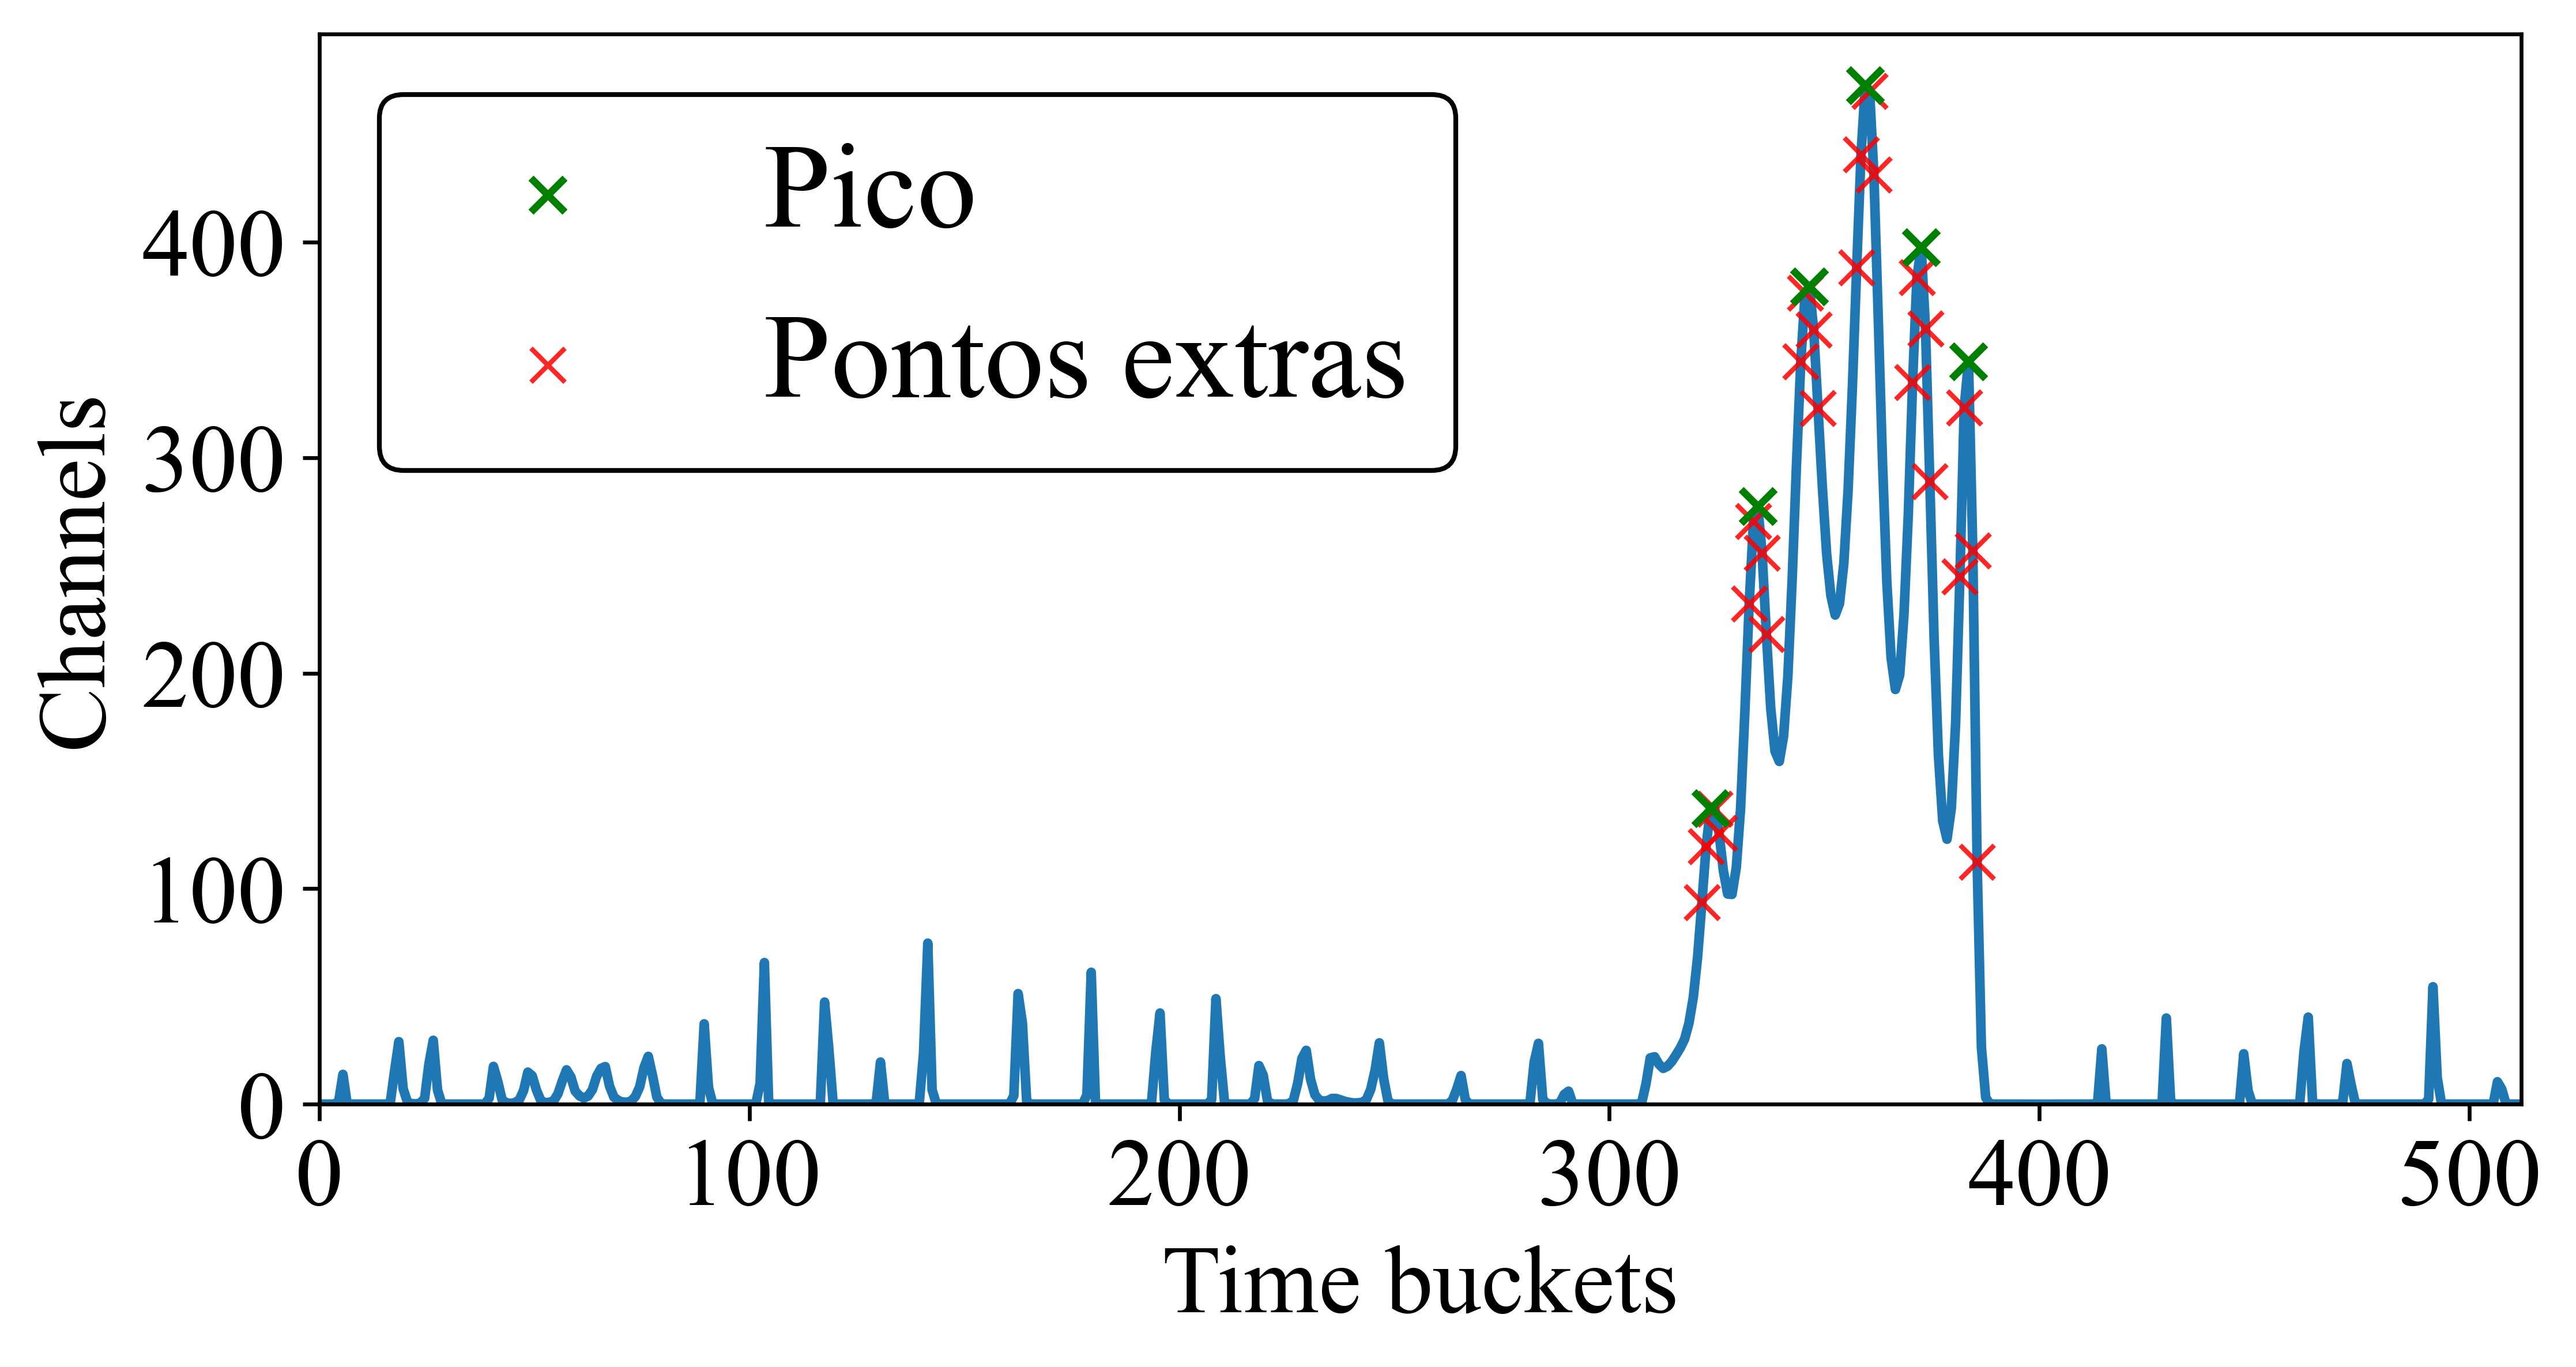
\includegraphics[scale = 0.6]{figs/np_ex1.png}
    \caption{Sinal após a deconvolução que mostra o pico identificado mais os pontos adicionais que irão facilitar o trabalho da rede neural (evitar o desbalanço de classe). Foram acrescentados 2 pontos à esquerda e à direita.}
    \label{fig:n_peaks_exs}
\end{figure}

\par A rede construída é a sequência de uma convolução com filtros de tamanho 13 e \textit{same padding} seguida de \textit{Max-Pooling} e uma camada \textit{fully-connected}. Os neurônios na camada FC são seguidas pela função de ativação sigmoid, que limita os neurônios da camada de saída no intervalo $[0,1]$. Assim, nesse caso nós trocamos a função custo \textit{mean squared error} pela \textit{binary cross entropy} \cite{mlbook}. Essa rede tem um total de 263.104 parâmetros treináveis. Para o treino foram usados sinais que possuíam entre 1 e 6 picos resultantes da saída do algoritmo \textsc{peak\_finder} do SciPy, o que resultou em 120.024 dados para o treino e 30.006 para validação. A escolha pelos picos identificados pelo \textsc{peak\_finder} ao invés do algoritmo de identificação do TSpectrum é devido a uma maior flexibilidade de ajuste fino do algoritmo, tornando a identificação de picos muito melhor\cite{FORTINO2022166497}. O treino também foi realizado por uma GPU NVIDIA Tesla P100 e durou cerca de 8 minutos com 12 \textit{epochs}. A arquitetura da rede está na figura \ref{fig:arq:n_peaks} e os resultados do treino estão na figura \ref{fig:n_peaks_results}.

\begin{figure}[H]
    \centering
    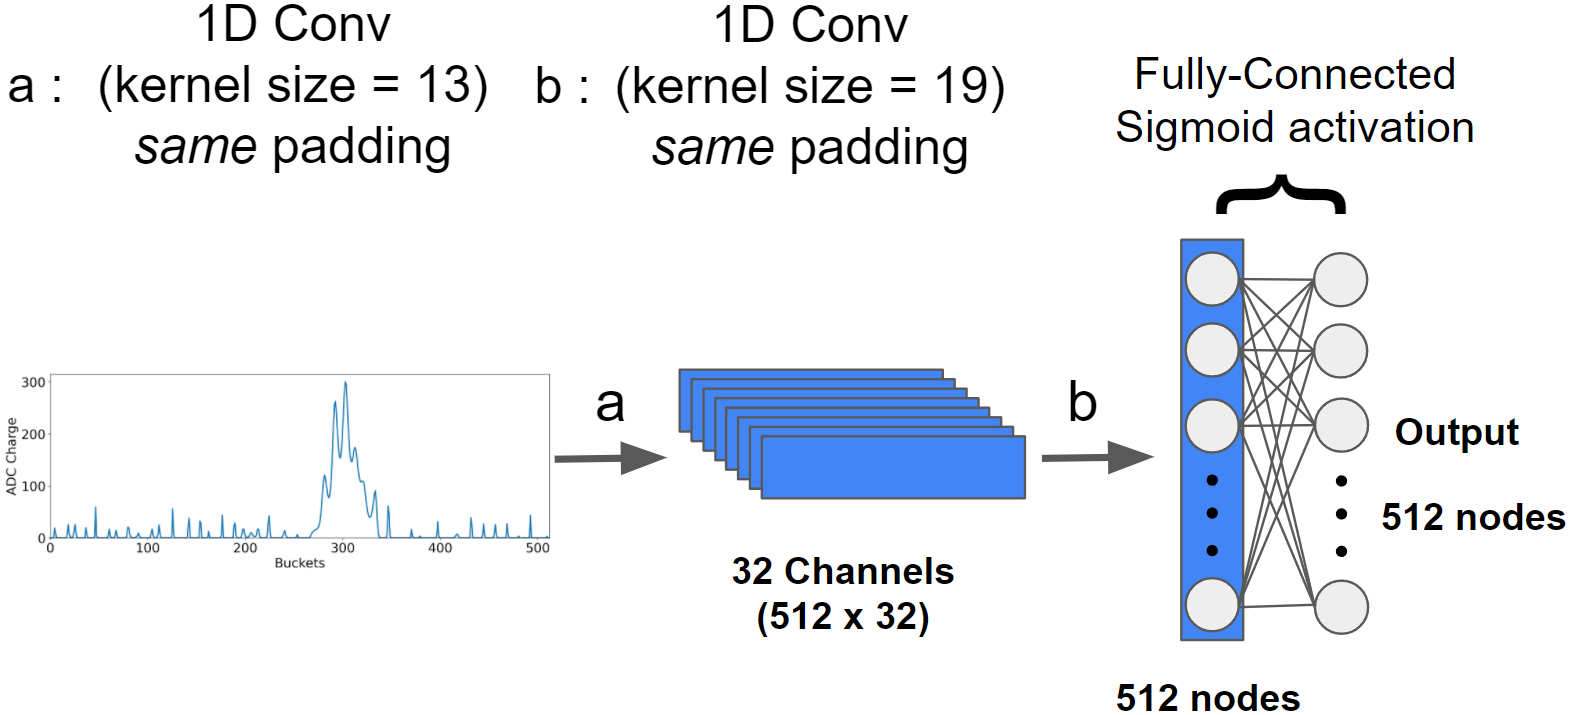
\includegraphics[scale = 0.35]{figs/n_peaks.png}
    \caption{Arquitetura da rede neural que faz o recorte das regiões com picos. O vetor de entrada deve ter dimensionalidade 512 x 1.}
    \label{fig:arq:n_peaks}
\end{figure}

\begin{figure}[H]
\centering
    \begin{subfigure}[t]{0.49\textwidth}
        \centering
        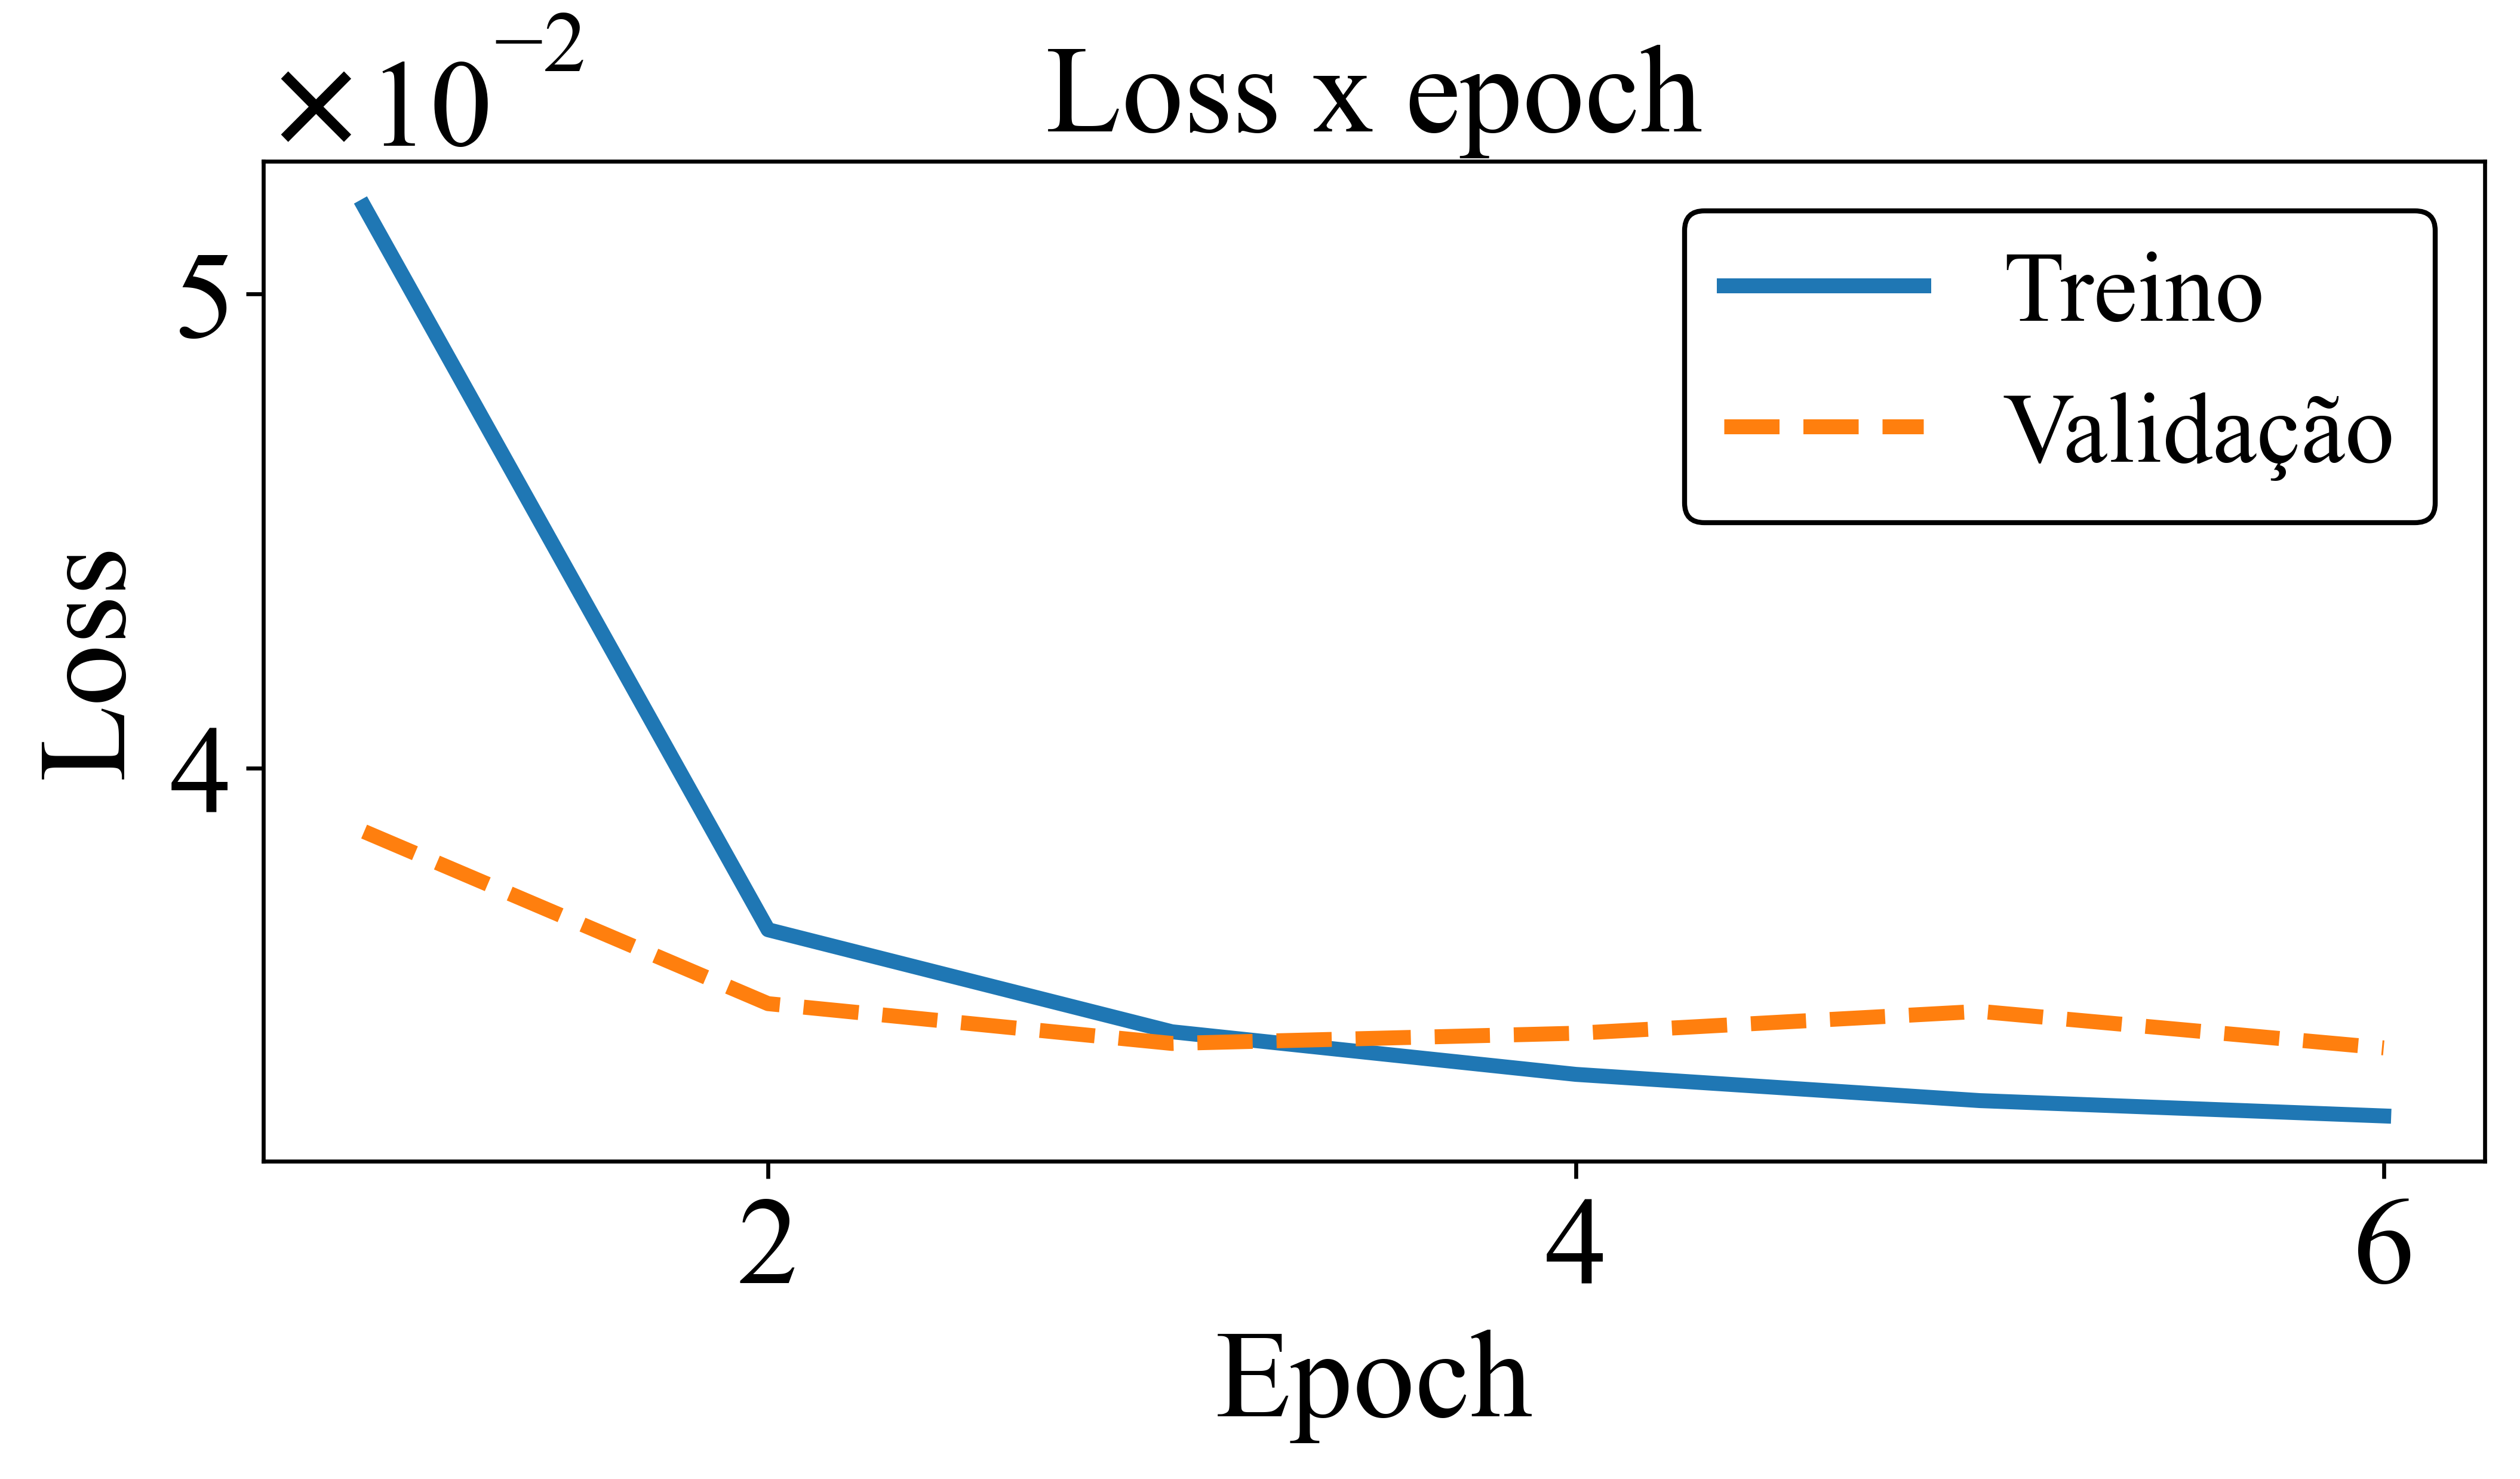
\includegraphics[scale=0.42]{figs/n_peaks_loss.png}
        \caption{Loss dos dados de treino (linha contínua) e dos dados de validação (linha tracejada) em função da epoch.}
        \label{subfig:n_peaks_loss}
    \end{subfigure}%
    \hfill
    \begin{subfigure}[t]{0.46\textwidth}
        \centering
        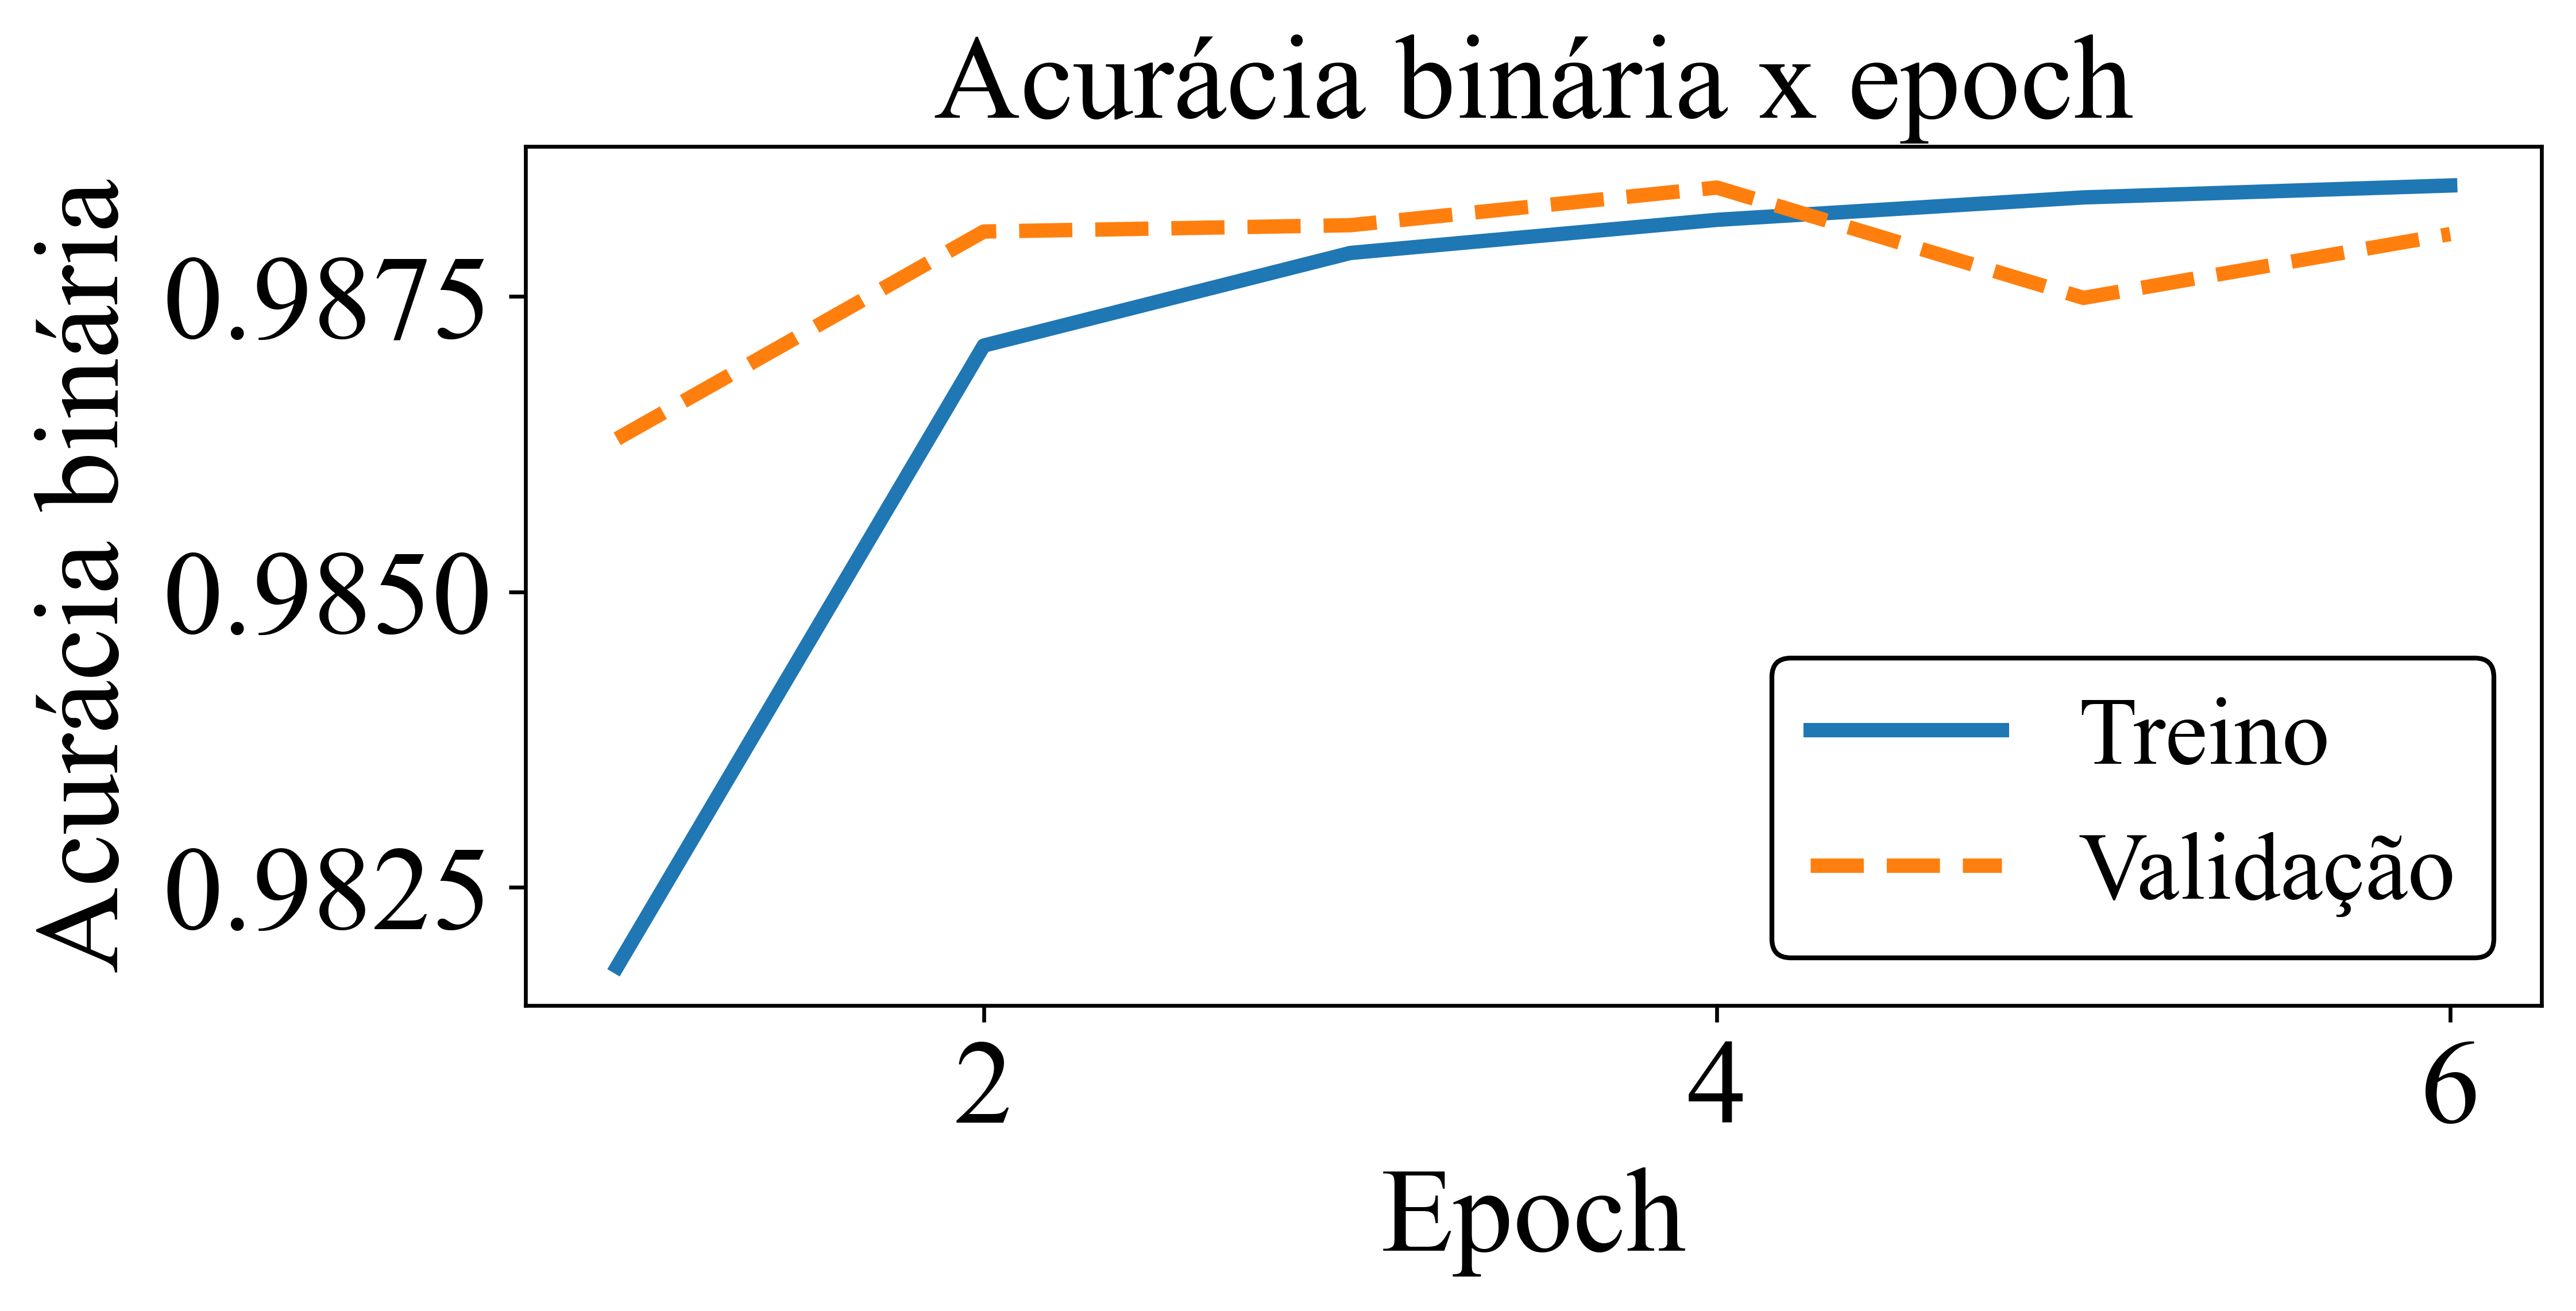
\includegraphics[scale=0.42]{figs/n_peaks_metric.png}
        \caption{Acurácia binária dos dados de treino (linha contínua) e dos dados de validação (linha tracejada) em função da epoch.}
        \label{subfig:n_peaks_metric}
    \end{subfigure}
\caption{Resultados do treino da rede neural dada pela figura \ref{fig:arq:n_peaks}.}
\label{fig:n_peaks_results}
\end{figure}

\par A saída da rede neural é um vetor de tamanho 512 com valores entre 0 e 1, onde valores maiores que 0.5 são considerados como pertencentes à um pico. Com as regiões identificadas podemos fazer uma média ponderada com o espectro de entrada para achar o centróide. O tempo de processamento da rede neural é de 150.030 sinais em cerca de 4.11 segundos (aproximadamente 36.500 sinais por segundo). Para determinar os picos a partir da saída da rede neural, o tempo é de aproximadamente 4.3 segundos, onde o algoritmo pode ser ainda mais rápido se for paralelizado. Resultados para picos identificados pela rede neural em comparação com o algoritmo \textsc{peak\_finder} estão na figura \ref{fig:exs_n_peaks}.

\begin{figure}[H]
\centering
    \begin{subfigure}[b]{0.49\textwidth}
        \centering
        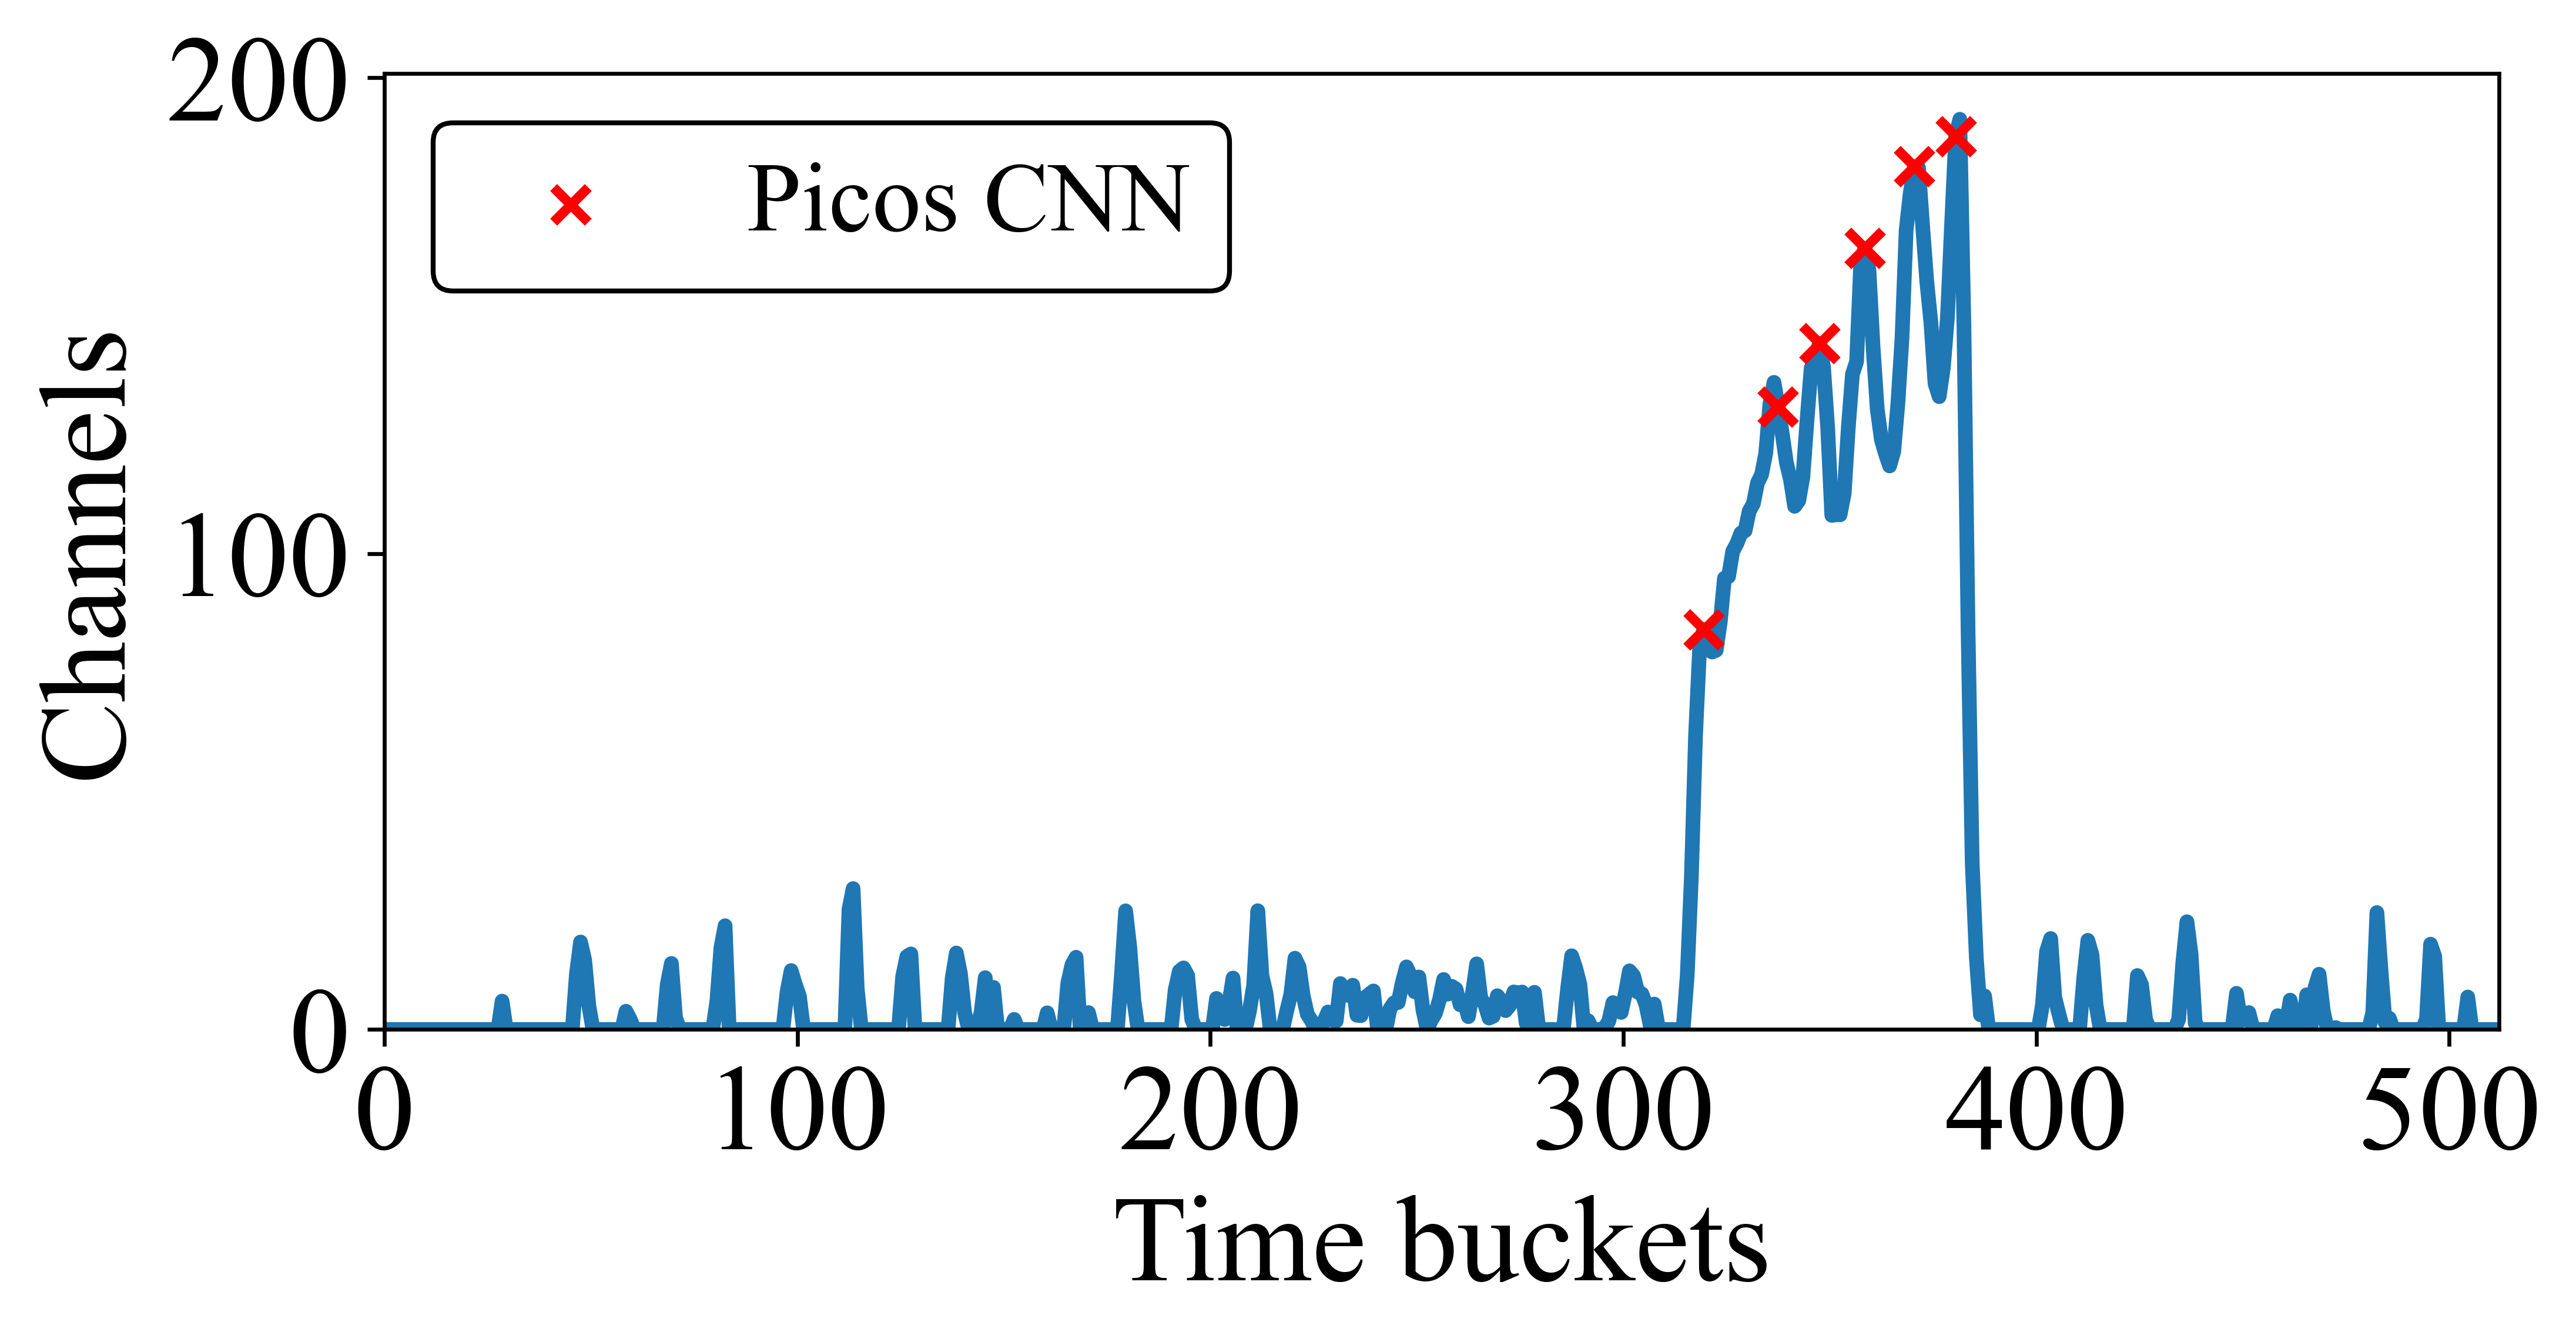
\includegraphics[scale=0.425]{figs/np_exs1.png}
        \caption{}
        \label{subfig:exs_n_peaks_1}
    \end{subfigure}%
    \hfill
    \begin{subfigure}[b]{0.465\textwidth}
        \centering
        \includegraphics[scale=0.425]{figs/np_exs2.png}
        \caption{}
        \label{subfig:exs_n_peaks_2}
    \end{subfigure}
    \begin{subfigure}[b]{0.49\textwidth}
        \centering
        \includegraphics[scale=0.425]{figs/np_exs3.png}
        \caption{}
        \label{subfig:exs_n_peaks_3}
    \end{subfigure}%
    \hfill
    \begin{subfigure}[b]{0.465\textwidth}
        \centering
        \includegraphics[scale=0.425]{figs/np_exs4.png}
        \caption{}
        \label{subfig:exs_n_peaks_4}
    \end{subfigure}
\caption{Exemplos de identificação de picos usando a rede neural, em comparação com a identificação feita pelo algoritmo presente no SciPy, mostrada na figura \ref{fig:arq:n_peaks}. Os centroides identificados pela rede neural estão em vermelho, e os centroides identificados pelo SciPy estão em verde. Em azul está o espectro sem fundo após a deconvolução, resultantes }
\label{fig:exs_n_peaks}
\end{figure}

\par Para determinar carga acumulada $Q_i$ de cada ponto associado à cada centroide $i$, foi usada a relação

\begin{equation}\label{eq:carga_acumulada_ml}
	Q_i = \sum_{i - 2}^{i + 2}f(t_i)\alpha_\sigma,
\end{equation}
%
onde $f(t_i)$ é a amplitude do espectro no \textit{time bucket} $t$ da posição $i$ e $\alpha_\sigma$ é uma constante real para calibrar o valor da área em função do sigma dos pulsos. Seu valor foi determinado de tal forma que, a área do pulso calculado a partir da integral da gaussiana ajustada deve ser igual à somatória dos 5 pontos que compõe o pulso (o centróide somado simetricamente com dois à esquerda e à direita) multiplicado pelo fator $\alpha_\sigma$. O valor de $\alpha_\sigma$ determinado foi tal que $\alpha_\sigma$  = 1,2.

%, que foi determinado empiricamente como $\alpha_\sigma$ = 1.2.

\par Uma vez tendo determinado as três redes neurais, devemos ainda verificar o acoplamento das redes, a fim de analisar a qualidade dos algoritmos e os tempos de execução, para comparar com os algoritmos discutidos nas subseções \ref{subsec:pulses_baseline} e \ref{subsec:pulses_deconv}.


\subsection{Acoplando as redes neurais}

%\par Com a rede que prevê o fundo e a que faz a deconvolução funcionando podemos agora testar se acopladas elas geram resultados satisfatórios, verificando a qualidade da detecção de picos.
\par Usando novamente o TensorFlow 2 pode-se carregar as redes neurais discutidas nas subseções \ref{subsec:pulso_ml_fundo}, \ref{subsec:pulso_ml_deconv} e \ref{subsec:pulso_ml_peaks}, já treinadas e usar como se fosse uma única rede neural. Acoplando as três arquiteturas, temos a nova arquitetura mostrada na figura \ref{fig:arq:source_to_segmentation}. O \textit{input} da rede é o sinal cru sendo que o \textit{output} da rede neural é o um vetor de tamanho 1024, que possui a segmentação e o sinal após a deconvolução, pois as duas informações são necessárias para determinar os centróides.

\begin{figure}[H]
    \centering
    \includegraphics[scale = 0.35]{figs/arq_source_segmentation.png}
    \caption{Arquitetura da rede neural que faz a inferência da baseline, em seguida faz a deconvolução do espectro sem o fundo e por fim faz a segmentação do sinal. O resultado da segmentação e da deconvolução são concatenados na parte final da rede neural. O vetor de entrada deve ter dimensionalidade 512 x 1.}
    \label{fig:arq:source_to_segmentation}
\end{figure}

\par A rede final é apenas a sequencia das redes anteriores, ou seja, o espectro passa pelo cálculo da baseline, então o espectro original é subtraído dessa \textit{baseline} (colocando o valor mínimo em 0) para passar pela etapa da deconvolução e em seguida o sinal é segmentado. Na etapa final, o resultado da segmentação e da deconvolução são concatenados em um único vetor, para assim determinar os centroides. Pelo fato de cada parte ser treinada de modo separado não há necessidade de treinar a rede unificada, apenas carregar as variáveis das redes neurais treinadas de cada parte. A rede unificada possui 1.316.640 de parâmetros.

\par A saída da rede acoplada para o espectro após a deconvolução foi comparada com a saída de referência, que é o espectro após a deconvolução mostrado na subseção \ref{subsec:pulses_deconv}. Para uma análise comparativa quantitativa usamos os valores do erro médio absoluto, cujo valor médio para os 200.000 sinais, foi de 7.45 ADC Channels. Com relação à incerteza, ela foi estimada como o desvio padrão da diferença de cada time bucket do sinal tido como referência e o sinal após a rede neural acoplada. A incerteza é da ordem de 6\% da amplitude do sinal no ponto.

\par Com relação a eficiência em tempo, a rede neural da figura \ref{fig:arq:source_to_segmentation} processa 200.000 sinais em 12 segundos, usando a GPU NVIDIA Tesla P100. Somando esse tempo com a determinação dos centroides, que é de aproximadamente 4.3 segundos, o tempo total para processar 200 mil sinais é de cerca de 16.3 segundos, cerca de 90 vezes mais rápido que os métodos mostrados na seção \ref{sec:pulses_trad}. O resultado final dessa rede neural é a geração de pontos no espaço definidos pelos parâmetros, \textit{x}, \textit{y} e \textit{z}. Um evento, correspondente à uma reação nuclear no alvo ativo gera vários pontos formando o que chamamos de nuvens de pontos. Essas nuvens de pontos definem então a trajetória das partículas produzidas por uma reação nuclear. Exemplos da reconstrução das nuvens de pontos usando a rede neural da figura \ref{fig:arq:source_to_segmentation} são apresentados na figura \ref{subfig:ex_ev_4}.

\begin{figure}[H]
\centering
    \begin{subfigure}[b]{0.48\textwidth}
        \centering
        \includegraphics[scale=0.38]{figs/ex_ev_1.png}
        \caption{}
        \label{subfig:ex_ev_1}
    \end{subfigure}%
    \hfill
    \begin{subfigure}[b]{0.48\textwidth}
        \centering
        \includegraphics[scale=0.38]{figs/ex_ev_2.png}
        \caption{}
        \label{subfig:ex_ev_2}
    \end{subfigure}
    \begin{subfigure}[b]{0.48\textwidth}
        \centering
        \includegraphics[scale=0.38]{figs/ex_ev_3.png}
        \caption{}
        \label{subfig:ex_ev_3}
    \end{subfigure}%
    \hfill
    \begin{subfigure}[b]{0.48\textwidth}
        \centering
        \includegraphics[scale=0.38]{figs/ex_ev_4.png}
        \caption{}
        \label{subfig:ex_ev_4}
    \end{subfigure}
\caption{Exemplos de eventos reconstruídos através da análise dos sinais com machine learning. A seta vermelha indica o sentido do feixe. Diferentes nuvens de pontos (eventos) correspondem a diferentes trajetórias de partículas sendo produzidas por diferentes reações nucleares.}
\label{fig:ex_eventos}
\end{figure}

\par Com as redes neurais desenvolvidas, o consumo de tempo para o processamento dos pulsos diminuiu em cerca de 90 vezes em relação à algoritmos com programação tradicional mostrados na seção \ref{sec:pulses_trad}, abrindo possibilidades para a análise em tempo real de um experimento com alvo ativo usando grande granularidade (milhares de canais). Com as nuvens de pontos reconstruídas, pode-se extrair propriedades físicas dos eventos, processo que está descrito no capítulo \ref{chapter:point_cloud_analysis} a seguir.

\chapter{Análise das nuvens de pontos}\label{chapter:point_cloud_analysis}

\par As nuvens de pontos representam eventos de reações nucleares dentro do alvo ativo. O objetivo desta etapa, do ponto de vista computacional, foi de identificar \textit{clusters} (aglomerados) tridimensionais de pontos, que no caso do pAT-TPC (sem a presença de campo magnético) devem seguir um comportamento de trajetórias retilíneas. Já do ponto de vista físico, o objetivo é extrair as informações das reações nucleares (energia $E$, momento $\vec{p}$ e comprimento $L$) a partir das trajetórias das partículas. Para tanto, foi necessário distinguir cada trajetória identificada e determinar o vértice da reação. Após a identificação de cada trajetória, foram selecionados os eventos correspondentes ao canal de reação do breakup cujas partículas seguiam uma trajetória específica.

\par Assim como no capítulo \ref{chapter:sinais}, esse capítulo descreve o uso de algoritmos de machine learning para a análise, determinação e identificação das trajetórias a partir das nuvens de pontos. Os algoritmos usados foram tanto não supervisionados (algoritmos de \textit{clustering}) e supervisionados (redes neurais), com diferentes objetivos.

\par Na seção \ref{sec:forcabruta} está mostrado o processo de identificação de trajetórias (\textit{tracking}) com algoritmo de machine learning não supervisionados. Na seção \ref{subsec:pointnet} estão mostradas alternativas com outros algoritmos de machine learning, que não foram utilizadas para a análise dos dados, mas que abrem um grande leque de possibilidades para estudos futuros.



\section{Identificação de trajetórias}\label{sec:forcabruta}

\par Uma vez reconstruídas as nuvens de pontos de cada evento, é necessário classificar cada uma das trajetórias (\textit{tracks}) das partículas dentro do gás. A figura \ref{subfig:exemplo_1} mostra um exemplo de uma nuvem de pontos. A classificação das trajetórias pode ser realizada a partir de algoritmos de machine learning não supervisionados. Nessa figura é notável ao olho humano que os pontos formam estruturas de aglomerados. Pode-se associar uma reta a essas estruturas que corresponderiam a trajetória das partículas dentro do alvo gasoso. Essa retas foram identificadas com algoritmos de \textit{clustering}. Devemos ressaltar que as nuvens de pontos não tem um tamanho ou numero de pontos definidos. O número de pontos pode variar de 30 até cerca de 200, não considerando pontos \textit{outliers} (não pertencem a nenhum aglomerado).

\par Para melhor definirmos os aglomerados devemos primeiramente eliminar ou diminuir os \textit{outliers}. Para tanto, foram usados dois filtros. O primeiro filtro exclui pontos baseado em sua carga, colocando um limiar onde pontos com carga $Q$ $<$ 110 são descartados. O segundo filtro, chamado de \textsc{outlier removal}, elimina pontos considerados \textit{outliers} globais (que não fazem parte de nenhum aglomerado), de modo que, caso um ponto não possua um número mínimo de vizinhos $n_{or}$ = 4 em um raio de distância tridimensional $d_{or}$ = 12 mm, então ele é descartado. O \textsc{outlier removal} está presente na biblioteca Open3D \cite{open3d} no Python e funciona excluindo pontos muito isolados uns dos outros.

\par Existem diversas opções de algoritmos de identificação de cluster disponíveis, como o \textit{Density-based spatial clustering of applications with noise} (\textsc{DBSCAN}) \cite{dbscan}, porém nossa escolha foi baseada na performance em tempo. Portanto, o algoritmo usado foi o \textit{Hierarchical DBSCAN} (\textsc{HDBSCAN}) \cite{hdbscan1, hdbscan2}. O algoritmo tem como entrada a nuvem de pontos e parâmetros esperados para a densidade dos aglomerados presentes no conjunto de pontos, como a densidade mínima e máxima de pontos nos aglomerados. O algoritmo retorna vetores que tornam possíveis a identificação dos diferentes aglomerados. Os aglomerados passam por um ajuste por mínimos quadrados para determinar o versor e um ponto arbitrário que determinam a reta tridimensional relacionada com a trajetória. A figura \ref{subfig:antes_clustering} mostra o resultado da aplicação do \textsc{HDBSCAN} na nuvem de pontos mostrada na figura \ref{subfig:exemplo_1}. As nuvens de pontos reconstruídas não possuem, em certos casos, densidade de pontos o suficiente para resultar em 100\% de acurácia de identificação correta de todas as trajetórias do evento.


\begin{figure}[H]
\centering
    \begin{subfigure}[b]{\textwidth}
        \centering
        \includegraphics[scale = 0.4]{figs/clustering_ex_1.png}
        \caption{Exemplo de evento analisado. Os pontos em azul são das partículas detectadas pelo TPC, a seta vermelha indicando o sentido do feixe e o TPC está representado pelo cilindro cinza.}
        \label{subfig:exemplo_1}
    \end{subfigure}%
    \hfill
    \begin{subfigure}[t]{0.45\textwidth}
        \centering
        \includegraphics[scale=0.25, width=.95\columnwidth]{figs/clustering_ex_2.png}
        \caption{Evento com as identificações sem a correção. As três retas de cores amarela, verde e azul são de um único cluster.}
        \label{subfig:antes_clustering}
    \end{subfigure}%
    \hspace{0.5cm}
    \begin{subfigure}[t]{0.45\textwidth}
        \centering
        \includegraphics[scale=0.25, width=.95\columnwidth]{figs/clustering_ex_3.png}
        \caption{Evento corrigido. Agora o evento possui as duas retas corretas, a azul e a verde.}
        \label{subfig:depois_clustering}
    \end{subfigure}
\caption{Sequência de análise de um evento. Em \ref{subfig:exemplo_1} temos o evento que é recebido para ser analisado, em \ref{subfig:antes_clustering} temos o mesmo evento após o \textsc{HDBSCAN} (antes da correção) e \ref{subfig:depois_clustering} mostra depois da correção. As cores das retas são arbitrárias e servem apenas para a diferenciação.}
\label{fig:3d_examples}
\end{figure}

\par O \textsc{HDBSCAN} pode apresentar falhas na analise dos aglomerados e identificação das trajetórias, como visto na figura \ref{subfig:antes_clustering}, em que, por exemplo, em que uma nuvem de pontos acaba sendo identificada e dividida em três clusters muito próximos. Para esses casos, foi aplicada uma correção da saída do \textit{clustering}. A correção foi feita comparando em pares todos os aglomerados resultantes do algoritmo e unificando os subconjuntos muito semelhantes \cite{artigo}. Do ponto de vista computacional, esse problema é abordado avaliando a semelhança entre dois aglomerados usando métricas, como a distância de Jaccard \cite{jaccard_distance} e o coeficiente de silhueta \cite{silhueta}. A correção feita se dá em duas etapas: primeiro comparando os versores entre duas retas e depois verificando se a condição da equação \ref{criterio_clustering} é satisfeita. Caso a diferença absoluta entre os ângulos com relação ao versor (0, 0, 1) (direção do feixe de $^{17}$F) seja menor que 9º (determinado empiricamente verificando a eficiência da correção), então as duas retas serão combinadas se obedecerem a condição dada por

\begin{equation}\label{criterio_clustering}
    \sum_{i = 0}^{N_1}\frac{d_{i2}}{N_1} < \alpha \space d_{min}, 
\end{equation}
%
onde $N_1$ é o número de pontos da reta 1, $d_{i2}$ a distância euclidiana do ponto $i$ da reta 1 em relação à reta 2, $\alpha$ é um parâmetro com valor a ser escolhido e $d_{min}$ é a distância mínima do ponto a reta. Os valores foram determinados empiricamente, verificando a eficiência da correção para a próxima etapa, e seus valores são tais que $\alpha$ = 1.75 e $d_{min}$ = 15 mm. A figura \ref{subfig:depois_clustering} mostra o resultado da correção baseada nesses critérios no resultado anterior mostrado na figura \ref{subfig:antes_clustering}.

\par Após a correção, é necessário classificar cada reta como sendo feixe, ou uma partícula originada de uma reação nuclear. O feixe incide na câmara possui um ângulo muito pequeno com relação ao versor (0, 0, 1), que é o versor de incidência do feixe. Além disso, mesmo que o ângulo seja pequeno, a reta do feixe cruza o plano da janela do TPC próximo ao ponto mais provável da entrada o feixe. Por sua vez, o ponto mais provável foi determinado usando a posição média da projeção dos pontos de um conjunto de eventos no plano \textit{x-y}. A posição inicial mais provável obtida para o feixe foi $x_f$ = -3.4 (6.7) mm e $y_f$ = -0.9 (6.3) mm. A incerteza é alta devido às dimensões do feixe (aproximadamente 5 mm). Portanto, se o ângulo entre o versor $\hat{v}_i$ de uma reta $r_i$ for menor que 5° (determinado de modo empírico novamente) e a distância $d$ entre o ponto $P_i$ que intercepta o plano e o ponto ($x_f$, $y_f$, 0) for menor que 15 mm (pouco mais que duas vezes a incerteza de cada ponto), então a reta foi considerada como o feixe do evento. No caso de não satisfazer essas condições, então ela foi classificada como uma possível partícula originada da reação do feixe com o gás.

\par É importante ressaltar que alguns eventos são caracterizados por apenas uma trajetória reta não sendo possível determinar o projétil ou o ejétil. Um exemplo desse tipo de evento é mostrado na figura \ref{fig:exemplo_sem_feixe}. Nesse caso, foi necessário assumir as propriedades da reta mais provável para o feixe, ou seja, uma reta que passe pelo ponto ($x_f$, $y_f$, 0) e que tenha um versor (0, 0, 1).

%\par Importante notar que há eventos que não possuem projétil ou ejétil ($^{17}$F por exemplo), como mostrado na figura \ref{fig:exemplo_sem_feixe}. Neste caso, foi necessário assumir as propriedades da reta mais provável para o feixe, ou seja, precisa passar pelo ponto ($x_f$, $y_f$, 0) e ter versor (0, 0, 1).

\begin{figure}[H]
    \centering
    \includegraphics[scale = 0.65]{figs/Figure_12.png}
    \caption{Evento em que não foi identificado o feixe, apenas a partícula espalhada. O triângulo azul é o local calculado do vértice de reação dado pela equação \ref{eq:vertice_reacao}.}
    \label{fig:exemplo_sem_feixe}
\end{figure}

\par Para podermos selecionar um determinado tipo de reação precisamos primeiramente caracteriza-la. Uma reação nuclear é caracterizada pela incidência de partículas do feixe (em movimento), partículas do alvo (em repouso) e as partículas emergentes da reação. As partículas da reação são emitidas considerando uma determinada cinemática. Para determinarmos completamente a cinemática do evento foi necessário determinar o vértice da reação (ponto em que a reação ocorre) que corresponde ao ponto de cruzamento entre a trajetória da partícula e a direção do feixe. Portanto, o vértice de reação é o ponto médio do menor segmento de reta que conecta a trajetória da partícula espalhada ou emergente da reação e o feixe, no ponto de menor distância entre as retas. O vértice é de grande importância para que possamos determinar o tipo de reação nuclear que ocorreu. Para deduzir uma expressão que possamos usar para determinar o vértice da reação temos que considerar as seguintes equações das retas $\vec{P_1}$ e $\vec{P_2}$, que podem ser retas quaisquer (que serão atribuídas às partículas), como vetores:

\begin{equation}
\begin{split}
        &\vec{P_1} = \vec{A_1} + \vec{V_1} * t_1 \\
        &\vec{P_2} = \vec{A_2} + \vec{V_2} * t_2,
\end{split}
\end{equation}
%
onde $\vec{A_1}$ e $\vec{A_2}$ são pontos arbitrários que pertencem as retas 1 e 2, respectivamente, $\vec{V_1}$ e $\vec{V_2}$ são os versores, $t_1$ e  $t_2$ são os hiperparâmetros escalares das retas.

\par Como o vértice de reação é o ponto médio do menor segmento de reta que conecta as duas retas, então é preciso determinar o versor $\vec{V_c}$ desse segmento de reta. Então, $\vec{V_c}$ é dado por

\begin{equation}\label{eq:versor_menor_dist}
    \vec{V_c} = \frac{\vec{V_1} \times \vec{V_2}}{\left | \vec{V_1} \times \vec{V_2} \right |}.
\end{equation}

Podemos então construir a reta $\vec{P_3}$ que possui as características do menor segmento de reta que conecta $\vec{P_1}$ e $\vec{P_2}$. Essa reta deve começar no ponto de menor distância da reta 1 e terminar no ponto de menor distância da reta 2. Ou seja, tem-se o seguinte sistema linear:

\begin{equation*}
    \vec{A_2} + \vec{V_2} * \tilde{t_2} = \vec{A_1} + \vec{V_1} * \tilde{t_1} + \vec{V_c} * \tilde{t_3}.
\end{equation*}

Rearranjando temos que

\begin{equation}\label{eq:sistema_vertice}
    \vec{V_1} * \tilde{t_1} - \vec{V_2} * \tilde{t_2} + \vec{V_c} * \tilde{t_3} = \vec{A_2} - \vec{A_1},
\end{equation}
%
onde $\tilde{t_1}$, $\tilde{t_2}$ e $\tilde{t_3}$ são os hiperparâmetros a serem determinados. Caso $\vec{V_1}$ seja paralelo à $\vec{V_2}$, então não há solução (não há vértice de reação, ou seja, não há uma reação nuclear em comum entre a partícula e o feixe analisado). Com a solução do sistema pode-se obter os pontos de menor distância nas duas retas:

\begin{equation}
\begin{split}
        &\vec{P_1} = \vec{A_1} + \vec{V_1} * \tilde{t_1} \\
        &\vec{P_2} = \vec{A_2} + \vec{V_2} * \tilde{t_2}.
\end{split}
\end{equation}

\par Com isso, é possível determinar que o vértice de reação $\vec{V_r}$ é dado por

\begin{equation} \label{eq:vertice_reacao}
    \vec{V_r} = \frac{1}{2}(\vec{P_1} + \vec{P_2}).
\end{equation}

\par Pode-se definir a distância de máxima aproximação $d_{max}$ das retas, dada por:

\begin{equation} \label{eq:menor_dist_retas}
    d_{max} = \left | \vec{P_1} - \vec{P_2} \right |.
\end{equation}

% \par No caso em que $\vec{V_c}$ em \ref{eq:versor_menor_dist} é zero, então as retas analisadas são paralelas. Nesse caso não há vértice de reação e a distância de máxima aproximação é dada por

\par Da equação \ref{eq:menor_dist_retas} foi estabelecido um limite superior para $d_{max}$ tal que valores menores que esse limite indicam uma reação nuclear em comum entre a partícula e o feixe. O valor foi determinado de forma empírica analisando diversos eventos. O valor então foi definido como $d_{max}^{sup}$ = 25 mm. Trajetórias cuja distância máxima de aproximação excedia $d_{max}^{sup}$, então a trajetória é descartada. Além disso, é necessário garantir que a reação ocorreu dentro da área efetiva da câmara e para tanto impomos os limites: $|x| < $ 140mm, $|y| < $ 140mm e $|t| < $ 512.

\par Para completar essa etapa, foi necessário determinar a carga total $Q_\text{T}$ e o comprimento $L$ da trajetória. A carga total $Q_\text{T}$ é definida como

\begin{equation}\label{eq:carga_acumulada}
	Q_\text{T} = \sum_{i = 1}^{N} Q_i,
\end{equation}
%
onde $Q_i$ é a carga do i-ésimo ponto de um conjunto com $N$ pontos. O comprimento é definido como

\begin{equation}\label{eq:comprimento_trajetoria}
	L = \max \left\{  d_{i,\vec{V_r}} \right\},
\end{equation}
%
onde $d_{i, \vec{V_r}}$ é distância entre o ponto $i$ pertencente a trajetória até o vértice de reação $\vec{V_r}$.

\par Essa não foi a única abordagem utilizada nesse trabalho para a determinação do vértice e portanto para a determinação da reação nuclear. Na seção \ref{sec:abordagens_alternativas} mostramos alternativas para se buscar, com as nuvens de pontos crua, eventos específicos que ocorreram no experimento, sem ter que previamente buscar trajetórias e também outros usos de machine learning para a análise.

\section{Abordagens alternativas}\label{sec:abordagens_alternativas}

\par  O objetivo da análise das nuvens de pontos foi de selecionar eventos que possuíam três trajetórias, uma sendo o feixe, e as outras duas de partículas que surgiram da reação nuclear do feixe com o gás.

\subsection{Identificação de eventos com machine learning}\label{subsec:pointnet}

\par Para evitar o processo de busca de aglomerados nas nuvens de pontos que não possuem eventos de interesse (como o breakup), é possível usar redes neurais supervisionadas capazes de processar nuvens de pontos tridimensionais. A rede neural usada para esse processo chama-se \textsc{PointNet} \cite{qi2016pointnet}. A \textsc{PointNet} é uma rede neural desenvolvida para classificar e segmentar imagens em 3D utilizando nuvens de pontos que representam uma forma 3D do objeto. A arquitetura dessa rede neural está na figura \ref{fig:aqr:pointnet}.

\begin{figure}[H]
    \centering
    \includegraphics[scale = 0.22]{figs/pointnet_arch.png}
    \caption{Arquitetura da \textsc{PointNet}. A rede de classificação tem os dados de entrada com $n$ pontos com 3 coordenadas, onde são aplicadas sequências de transformação que são agregadas por uma camada de \textit{max pooling}. A saída é a classificação para $k$ classes possíveis. A rede de segmentação é uma extensão da rede de classificação, classificando ponto a ponto a nuvem de pontos, em $m$ classes possíveis. Mais detalhes sobre a arquitetura podem ser encontrados na Ref. \cite{qi2016pointnet}.}
    \label{fig:aqr:pointnet}
\end{figure}

\par A \textsc{PointNet} é uma rede neural capaz de processar nuvens de pontos, entendendo que a estrutura dos dados é invariante à troca de pontos e invariante sobre transformações (rotação e translação) \cite{RF_pc}, pode ser usada tanto para classificação quanto segmentação semântica de nuvens de pontos \cite{qi2016pointnet}. A classificação é realizada para a nuvem de pontos como um todo, já a segmentação semântica é a classificação ponto a ponto da nuvem de pontos \cite{qi2016pointnet}. Para o uso da \textsc{PointNet} para classificação, foi criado um banco de dados para o treino da rede neural que tem como entrada a nuvem de pontos e como saída o número de trajetórias presentes no evento. Um dos pontos negativos da \textsc{PointNet} é a necessidade de que os dados de entrada tenham um tamanho fixo \cite{qi2016pointnet}. No caso dos dados desse trabalho, o número de pontos por evento não é  fixo. Para resolver isso, impomos para os nossos dados um tamanho fixo $n$ = 300 pontos para todas as nuvens de pontos. Eventos com menos pontos eram preenchidos com pontos repetidos da mesma nuvem para completar até o tamanho $n$. Eventos com menos do que 100 pontos e mais que 300 pontos foram descartados pois geralmente são ruídos e a saturação do detector devido à faíscas.

\par Para determinar o número de trajetórias nos eventos para o treino da rede neural, foi utilizado o estimador robusto (que estima quais as trajetórias presentes nas nuvens de pontos) que chamei de \textsc{prototype-RANSAC} (RANdom SAmple Consensus), que é uma variação do \textsc{RANSAC} \cite{ransac, artigo}. A escolha dele no lugar do \textsc{HDBSCAN} é pela melhor acurácia na identificação de trajetórias, apesar de ser cerca de 4 vezes mais lento. As nuvens de pontos (sem o acréscimo de pontos para a \textsc{PointNet}) ainda passam pelos dois filtros e critérios de correção mostrados na seção \ref{sec:forcabruta}. O algoritmo \ref{ransac_algo}, localizado no apêndice \ref{appendix:pransac}, mostra o funcionamento do \textsc{p-RANSAC}. O algoritmo seleciona dois pontos de modo aleatório e determina o versor $\hat{v}$ e o ponto $P_b$ que descrevem a única reta $r$ que passa pelos dois pontos. A reta é selecionada caso tenha um número mínimo de pontos $N_{min}$ = 24 (chamado de \textit{inliers}) e tenha o mínimo (com relação aos outros conjunto de pontos) da estimativa $C$ dada por \cite{artigo}

\begin{equation} \label{criterio_ransac}
    C = \sum_{i = 0}^{N} \frac{d_i ^2}{N},
\end{equation}
%
onde \textit{N} é o número total de pontos de uma reta e $d_i$ é a distância do i-ésimo ponto à reta. O número de iterações do algoritmo foi determinado empiricamente e o melhor valor encontrado foi de 700.

%\begin{algorithm}[H]
%    \caption{p-RANSAC}\label{ransac_algo}
%    \KwData{pointcloud, $N$, $d_{min}$, $N_{min}$}
%    \For{cada iteração $ i =1,2,\ldots, N$}{
%        Seleciona dois pontos da \textit{pointcloud} de modo aleatório (\textit{Random Sampling})\;
%        Estima versor $v$ e um ponto $P_b$ que passe pela reta \textit{r} formada pelos dois pontos\;
%        \For{cada ponto $P$}{
%            Calcula a distância $d$ do ponto à reta \textit{r}\;
%            \If{$d < d_{min}$}{
%			    Guarda $P$ como pertencente à $r$\;
%	        }
%	    }
%	    \If{Número de pontos de $r > N_{min}$}{
%	        Guarda $v$, $P_b$ e $C$\;
%	    }
%    }
%    Ordena as retas do menor para o maior $C$\;
%    \For{cada reta $r$ ordenada}{
%        \If{Número de pontos de $r > N_{min}$}{
%            Guarda $v$, $P_b$ e pontos $P$ $\in r$\;
%        }
%    }
%    \Return Retas $r$ selecionadas na última etapa\;
%\end{algorithm}

\par Para a saída foram escolhidos eventos que possuem de 0 até 5 trajetórias. Com os dados para a camada de saída construídos, a rede para classificação foi treinada, onde a função custo foi a \textit{categorical cross entropy} \cite{MSE_CEF_review} e o otimizador o ADAM \cite{ADAMAX}. A acurácia de 70\% quando concluído o treino. Exemplo do resultado da aplicação da rede neural em nuvens de pontos está na figura \ref{fig:pointnet_class_exs}.

\begin{figure}[H]
    \centering
    \includegraphics[scale = 0.5]{figs/ex1_pointnet_class.png}
    \caption{Nuvem de pontos que possui 3 trajetórias para serem identificadas e a rede neural de classificação calculou que haviam 3 trajetórias, o que indica um resultado correto do algoritmo. A seta vermelha indica a direção e o sentido do feixe.}
    \label{fig:pointnet_class_exs}
\end{figure}

\par Eventos com 4 ou 5 trajetórias ocorrem com uma frequência muito menor (menos que 5\% do total de dados) que eventos de 1 e 2 trajetórias (cerca de 85\% do total de dados), caracterizando o banco de dados com o problema de desbalanço de classe (já discutido na subseção \ref{subsec:pulso_ml_peaks}), o que pode ter prejudicado o treino para identificar eventos mais incomuns. 

%No dados do experimento desse trabalho não foi necessário utilizar essa rede neural, pois a etapa de identificação de trajetórias é rápida em comparação com a mesma etapa usando dados gerados com um alvo de maiores dimensões como o AT-TPC \cite{attpc, FORTINO2022166497}.

\subsection{Identificação de \textit{outliers}}

\par Um possível uso para a rede de segmentação semântica é para classificar pontos como \textit{inliers} ou \textit{outliers}, semelhante ao uso do algoritmo \textsc{outlier removal} da biblioteca Open3D \cite{open3d}. A diferença é que com a \textsc{PointNet} pode-se incluir \textit{outliers} locais (que fazem parte de outro aglomerado) \cite{RF_pc}, não apenas os globais para serem identificados.

\par Para a saída da rede neural, os pontos classificados como \textit{outliers} globais ou locais possuem valor 0 e pontos que são \textit{inliers} (pertencem à alguma trajetória) possuem valor 1. A rede de segmentação foi treinada, com a função custo sendo a \textit{binary cross entropy} e a mética a acurácia binária. A acurácia da rede foi de aproximadamente 93\%, se mostrando uma boa alternativa para eliminação de ruído nos eventos. A figura \ref{fig:pointnet_segment_exs} mostra o resultado da aplicação da rede de segmentação em uma nuvem de pontos.

\begin{figure}[H]
    \centering
    \includegraphics[scale = 0.4]{figs/pointnet_seg_ex1.png}
    \caption{Identificação de \textit{outliers} com a rede neural de segmentação. A rede neural foi capaz de identificar os \textit{outliers} desse evento com 95\% de acurácia.}
    \label{fig:pointnet_segment_exs}
\end{figure}

\par Existem outras redes neurais que são capazes de lidar com nuvens de pontos, como a \textsc{PointNet++} \cite{qi2017pointnetplusplus} e \textsc{Dynamic Graph CNN} \cite{graph_cnn}. Para a abordagem de identificação de trajetórias de forma direta, uma opção é utilizar a rede neural \textsc{ContrastNet} \cite{contrastnet}, pois a rede é capaz de fazer \textit{clustering} nos dados, retornando os diferentes aglomerados existentes nos dados. Num futuro, estamos pensando em utilizar esses tipos de ferramentas para realizar \textit{clustering} em nuvens de pontos em outros experimentos usando múltiplos canais de reação. No entanto, esse projeto esta além dos objetivos desta dissertação.

\par A classificação e ajuste de trajetórias apresentados no presente capítulo permitem obter informação da cinemática das reações nucleares e extrair as respetivas distribuições angulares. Essa análise é discutida no próximo capítulo.

\chapter{Resultados}\label{chapter:resultados}

\par Uma vez que tendo determinado as trajetórias das partículas e classificação das possíveis reações podemos selecionar a reação de interesse. Nesse nosso trabalho estamos interessados na reação de breakup, que corresponde a quebra do feixe de $^{17}$F em ${}^{16}\text{O}+p$ devido a interação com o alvo de $^{4}$He. Para que possamos estudar a reação de breakup de interesse precisamos obter a distribuição angular, ou seja, a probabilidade de que a reação aconteça em função do ângulo.
Nesse capítulo vamos descrever como podemos construir as distribuições angulares da reação de breakup do $^{17}$F a partir da análise das nuvens de pontos, como foi apresentado no capítulo \ref{chapter:point_cloud_analysis}.

\section{A cinemática da reação}\label{sec:identif_reac_nucl}

\par O processo de seleção e classificação de reações nucleares no alvo ativo é complexo e envolve várias etapas como: identificação de trajetórias e multiplicidade, determinação do vértice de reação, identificação de partículas e reconstrução da energia e ângulos da reação. As subseções a seguir descrevem essas etapas.

\subsection{Reconstrução do vértice da reação}
%\par Como foi descrito no capítulo \ref{chapter:point_cloud_analysis}, para analisar as nuvens de pontos (reações nucleares) é necessário identificar as trajetórias das partículas dentro do gás que formam linhas retas originadas num determinado vértice.
\par Para identificar e selecionar as reações nucleares que ocorrem dentro do alvo ativo é preciso identificar as trajetórias das partículas dentro do gás. O processo de determinação dessas trajetórias foi descrito na seção anterior, bem como a descrição de como obter o vértice da reação (que é o ponto em que efetivamente ocorre a reação nuclear). Isso é feito com estimadores robustos, como o algoritmo \textsc{p-RANSAC} (algoritmo \ref{ransac_algo}, apresentado no apêndice \ref{appendix:pransac} e também na referência \cite{artigo}), que é capaz de identificar os diferentes aglomerados mesmo na presença de \textit{outliers}.

\par Após a identificação e ajuste das trajetórias, é preciso determinar o vértice da reação para cada evento. O vértice é o ponto no espaço no qual ocorre a reação nuclear e pode ser determinado pela extrapolação das trajetórias na região central do alvo ativo. O ponto de interseção (ou mais próximo) entre duas retas é calculado como mostra a equação \ref{eq:vertice_reacao}. O feixe incide na parte central pelo eixo axial do alvo, região cujo ganho do micromegas é baixo para evitar a saturação dos sinais (devido à passagem do feixe). Portanto, para calcular o vértice de reação, é necessário extrapolar as trajetórias na região central. A partir do vértice, então, é possível calcular o comprimento $L$ da trajetória (dado pela equação \ref{eq:comprimento_trajetoria}), mesmo com a ausência de informação na região central.

\par Para alguns eventos foi possível observar as trajetórias do feixe e partículas produto da reação saindo de um mesmo vértice (ver figura \ref{subfig:res_exemplo_3_tracks}). Neste caso, o vértice corresponde ao ponto médio da interseção dessas trajetórias. Porém, na maioria dos casos não foi possível observar a trajetória do feixe por causa do baixo ganho nos pixels centrais do detector. Por exemplo, a figura \ref{subfig:res_exemplo_2_tracks} mostra só dois produtos de reação saindo do mesmo vértice. No entanto, o vértice pode ser reconstruido pela extrapolação das retas ajustadas às trajetórias das partículas. Por fim, o caso mais complicado é quando apenas foi identificada uma trajetória (ver figura \ref{subfig:res_exemplo_1_track}). Para reconstruir o vértice com apenas uma trajetória, é necessário assumir uma direção para a partícula do feixe. Assim como foi mencionado no capitulo 5, se assume que o feixe tem direção (0,0,1) e ponto de corte (-3.4,-0.9,0) que foi calculado usando a posição média da projeção dos pontos de um conjunto de eventos no plano \textit{x-y}. Portanto, o vértice corresponde ao ponto mais próximo da trajetória partícula com a trajetória assumida para o feixe.

\begin{figure}[H]
\centering
    \begin{subfigure}[b]{\textwidth}
        \centering
        \includegraphics[scale = 0.3]{figs/results_ex_3_tracks_41.png}
        \caption{Exemplo de reação nuclear onde foram identificadas três trajetórias.}
        \label{subfig:res_exemplo_3_tracks}
    \end{subfigure}%
    \hfill
    \begin{subfigure}[t]{0.45\textwidth}
        \centering
        \includegraphics[scale=0.5, width=.95\columnwidth]{figs/reac_alpha_alpha_num_212.png}
        \caption{Exemplo de reação nuclear onde foram identificadas duas trajetórias.}
        \label{subfig:res_exemplo_2_tracks}
    \end{subfigure}%
    \hspace{0.5cm}
    \begin{subfigure}[t]{0.45\textwidth}
        \centering
        \includegraphics[scale=0.5, width=.95\columnwidth]{figs/results_ex_1_track_num_220.png}
        \caption{Exemplo de reação nuclear onde foi identificada apenas uma trajetória.}
        \label{subfig:res_exemplo_1_track}
    \end{subfigure}
\caption{Exemplos de reações nucleares com as trajetórias identificadas. O vértice de reação é indicado por um \textit{X}, em preto. Há dois vértices de reação, pois foram calculados um para da partícula espalhada. As cores servem apenas para a diferenciação.}
\label{fig:res_tracks}
\end{figure}

%\par O limite de distância dos vértices calculados, para serem considerados pertencentes a mesma reação, foi de 20 mm.
%\par Importante notar que o aglomerado identificado de cor azul não possui pontos na perto da parte central da câmara, pois o ganho da eletrônica do micromegas na parte central é menor em comparação com a região não central.

\par Além da trajetória, a energia das partículas também é um parâmetro importante para a classificação e determinação da reação nuclear.

\subsection{Reconstrução da energia das partículas}

%\par Para reconstruir a energia das partículas, foi necessário utilizar do comprimento da trajetória e também do poder de freamento (\textit{stopping power}) \cite{DETC_TELE} da partícula no gás. O \textit{stopping power} depende principalmente na carga da partícula incidente e na propriedades do gás como a pressão e temperatura.

\par Numa primeira aproximação, a energia da partícula associada a uma determinada trajetória pode ser estimada a partir da equação \ref{eq:carga_acumulada}, onde são somadas todas as cargas dos pontos da trajetória. Porém, a eficiência de detecção depende da energia depositada pela partícula no gás. Da mesma forma, alguns pontos das trajetórias das partículas podem estar ausentes devido ao processamento eletrônico ou mesmo na reconstrução das nuvens de pontos. Outra forma de obtermos (determinarmos) a energia da partícula é a partir da relação do comprimento da trajetória e a energia perdida pela partícula dentro do gás (poder de freamento ou stopping power). A perda de energia da partícula no gás depende principalmente da carga da partícula incidente e das propriedades do gás, como a pressão e temperatura. Essa energia perdida no gás foi calculadao usando o programa \textsc{lise++} \cite{lise++} e os respectivos comprimentos das trajetórias associadas a partículas como $^{16}$O, alfas e prótons num gás de $^4$He à uma pressão de 350 Torr. Partículas diferentes perdem energias de forma diferente e, portanto, têm alcances diferentes dentro do gás em função de sua energia. A figura \ref{fig:alcance_vs_energia} mostra o alcance em função da energia do $^{17}$F, $^{16}$O e próton, onde é possível ver a diferença de alcance das partículas dentro gás, especialmente entre as partículas pesadas ($^{17}$F, $^{16}$O) e o próton.

%\par Numa primeira aproximação, a energia da trajetória pode ser estimativa a partir da equação \ref{eq:carga_acumulada}, onde são somadas todas as cargas acumuladas dos pontos das trajetórias. Porém a eficiência de detecção depende da energia da partícula e algumas regiões das trajetórias podem não ser detectadas. Usando o LISE++ \cite{lise++} foi possível calcular o alcance das possíveis partículas ($^{16}$O e próton) dada as propriedades do alvo ($^4$He gasoso à uma pressão de 350 Torr). A figura \ref{fig:alcance_vs_energia} mostra o alcance em mm das partículas ($^{17}$F, $^{16}$O e próton) em função da energia em MeV. 

 \begin{figure}[H]
     \centering
     \includegraphics[scale = 0.85]{figs/alcance_vs_energia_2.png}\
     \caption{Alcance (mm) em função da energia (MeV) para o $^{17}$F, $^{16}$O e próton. A grande diferença está no próton que tem um alcance muito maior que os outros núcleos.}
     \label{fig:alcance_vs_energia}
 \end{figure}

\par Por exemplo, para determinar a energia cinética do $^{17}$F antes da reação nuclear, pode se usar a distancia entre a janela do detector e o vértice da reação. Para isso, o espaço no eixo $z$ foi discretizado, a fim de calcular a energia na posição da reação. O feixe, ao entrar no gás, possui energia inicial $E_0$ = 34.76 MeV, e perde energia ao atravessar o gás. A energia de reação $E_r$ é dada por

\begin{equation}
	E_r = E_0 - E_{loss},
\end{equation}
%
onde $E_{loss}$ é a energia do $^{17}$F depositada no gás que é calculada a partir da distancia $L$ até o vértice da reação. O comprimento $L$ é transformado em energia cinética usando uma tabela de \textit{stopping power}. Similarmente, a energia de outras partículas (e.g. alfa), que param completamente no gás, é calculado com o alcance da partícula (relativo ao vértice) e a sua respetiva tabela de \textit{stopping power}.

%\par A identificação do feixe ($^{17}$F) é feita a partir das propriedades geométricas das trajetórias, portanto fica evidente a diferença de alcance entre uma partícula de $^{16}$O e um próton, o $^{16}$O possui uma penetrabilidade muito menor que o próton.

\subsection{Determinação dos ângulos de reação}

\par Como mencionamos anteriormente, uma reação nuclear pode ser investigada a partir de sua distribuição angular. Portanto, um dos parâmetros importantes para a determinação da distribuição angular de uma determinada reação é exatamente o ângulo em que as partículas são emitidas.  

\par Para determinar os ângulos azimutal e axial (em coordenadas esféricas), foram feitos os ajustes tridimensionais dos aglomerados identificados (usando estimadores robustos ou algoritmos de clustering, como discutido no capítulo \ref{chapter:point_cloud_analysis}).

\par O ângulo de reação, para cada trajetória identificada, depende da determinação do versor de cada uma das trajetórias em relação ao versor do feixe. A partir das propriedades geométricas das trajetórias (versores das retas), são calculados os ângulos azimutal e axial com relação à direção em que o feixe incide na câmara (veja que a direção do feixe não necessariamente coincide com o eixo simétrico do TPC).

\par Para cada trajetória (reta) $i$, o ângulo azimutal $\phi_i$ é dado por

\begin{equation}
	\phi_i = \atantwo \left (\frac{y_i}{x_i} \right),
\end{equation}
%
onde $\atantwo$ é o arco-tangente calculado entre $-\pi$ e $\pi$, $y_i$ e $x_i$ são componentes $x$ e $y$ do versor da reta $i$. Para o ângulo polar $\theta$, ele é calculado a partir do produto interno entre o versor da reta e o versor do feixe, ou seja:

\begin{equation}
	\theta = \arccos \left (\frac{\vec{V_i} \cdot \vec{V_f}}{|\vec{V_i}| |\vec{V_f}|}  \right),
\end{equation}
%
onde $\vec{V_i}$ é o versor da reta $i$ e $\vec{V_f}$ é o versor do feixe.

\section{Identificação do canal de reação de breakup}

\par A grande vantagem do alvo ativo é a possibilidade de detectarmos partículas provenientes das mais diversas reações nuclear. Por outro lado, isso dificulta consideravelmente a análise pois precisamos identificar e classificar essas reações. Por exemplo, ao graficarmos o comprimento do alcance das partículas em função do ângulo, temos a presença de todas as partículas. Isso fica evidente ao olhar para a figura \ref{fig:comp_vs_ang}, que mostra um histograma bidimensional do comprimento da trajetória da partícula em função do ângulo de espalhamento (polar) no referencial de laboratório. Eventos de espalhamento em ângulos menores que 5 graus e reações na janela de entrada foram previamente removidos neste histograma.

%Primeiro é preciso entender os tipos de trajetórias identificados em eventos como os mostrados na figura \ref{fig:res_tracks}, que mostra as trajetórias de diferentes partículas no gás.

%\par Na figura \ref{subfig:res_exemplo_3_tracks} há a reação de breakup entre o $^{17}$F (trajetória de cor amarela) e o $^{4}$He gasoso. Os produtos da reação são o próton (trajetória de cor azul) e o $^{16}$O (trajetória de cor verde). Pela imagem é possível ver a diferença no comprimento das trajetórias, o próton possui um alcance maior que o $^{16}$O no gás.
%
%\par Na figura \ref{subfig:res_exemplo_2_tracks} há o espalhamento elástico do $^{17}$F (trajetória em cor verde) em alfa (trajetória de cor azul). Percebe que a trajetória da partícula alfa possui mais pontos e maior comprimento, enquanto a trajetória do $^{17}$F é mais curta e com um ângulo mais dianteiro.

%\par No caso da figura \ref{subfig:res_exemplo_1_track}, há uma única trajetória que não é possível de ser identificada visualmente. Identificar as partículas que originaram as trajetórias não é possível de se fazer diretamente (só com as informações descritas até este ponto).

% Para entender melhor a identificação de trajetórias, é necessário estudar todas as trajetórias identificadas. A figura \ref{fig:comp_vs_ang} mostra o histograma bidimensional do comprimento de cada trajetória em função do ângulo de espalhamento no referencial do laboratório.

\begin{figure}[H]
    \centering
    \includegraphics[scale = 0.5, width=\columnwidth]{figs/comp_vs_ang_n2_2.png}\
    \caption{Histograma de comprimento da trajetória no eixo $y$ e ângulo de espalhamento no eixo $x$.}
    \label{fig:comp_vs_ang}
\end{figure}

\par Pela figura \ref{fig:comp_vs_ang}, é possível perceber dois aspectos importantes sobre os dados. O primeiro é que o canal de reação correspondente ao espalhamento elástico e inelástico, é predominante no espectro. Devido ao fato do experimento ter sido realizado em cinemática inversa, o ângulo de espalhamento da partícula recuo depende do valor $Q$ da reação. Por exemplo, partículas alfa espalhadas elasticamente são detectadas em ângulos dianteiros menores que 90 graus. Os ângulos maiores que 90 graus neste caso correspondem a reações com $Q>0$, por exemplo a reação ($\alpha, p$). O segundo aspecto é a ausência de eventos abaixo de 50 mm, como é possível ver na figura \ref{fig:comp_vs_ang}. Essa ausência ocorre devido ao baixo ganho da região central do detector micromegas que limita a detecção de tracks menores do que 50 mm. Da mesma forma, a ausência de eventos na parte superior do histograma corresponde a limitação geométrica do TPC que possui um raio de 150 mm e comprimento de 500 mm.

% O primeiro é com relação à assimetria do ângulo de espalhamento. O desbalanço entre trajetórias com ângulo de espalhamento menor que 90º e maior que 90º ocorre pelo uso no referencial do laboratório. O ângulo de espalhamento no referencial do laboratório é metade do ângulo de espalhamento no referencial do centro de massa \cite{two_body_mec}. Ângulos maior que 90º na figura representam eventos de cinemática inversa. O segundo aspecto é a ausência de trajetórias na região central da figura. Essa ausência ocorre devido à limitações geométricas da câmara. Por exemplo, uma trajetória com ângulo de espalhamento de cerca de 90º não pode ter comprimento maior que 140 mm, pois o evento ocorre na região central da câmara e isso significa ultrapassar o limite geométrico do TPC.

\par O foco principal desse trabalho é identificar e selecionar 
os eventos correspondentes ao canal de breakup $\alpha$($^{17}$F,$^{16}\mathrm{O}+p$). Esse canal pode ser identificado a partir dos eventos com emissão de prótons. A figura \ref{fig:exemplo_proton_16O} mostra um exemplo de breakup de $^{17}$F em $^4$He observado no experimento.

\begin{figure}[H]
    \centering
    \includegraphics[scale = 1., width=0.75\columnwidth]{figs/evento_ex_run_261_evento_5853_2.png}
    \caption{Evento onde há a trajetória originada por um próton (trajetória em amarelo), onde percebe-se que seu comprimento vai até o limite geométrico da câmara (cilindro cinza transparente). O feixe está em azul e o $^{16}$O originou a trajetória em verde. É notável neste exemplo que a trajetória do próton é bem maior que o fragmento $^{16}$O.}
    \label{fig:exemplo_proton_16O}
\end{figure}

\par A seleção de eventos é feita aplicando vários gates (condições lógicas) para identificar os eventos com prótons. Isto pode ser feito num histograma da carga associada a uma trajetória em função de seu comprimento. A relação entre essas duas variáveis se dá por meio da expressão para o stopping power, onde o termo dominante da equação de Bethe Block \cite{leo1988techniques} em baixas energias pode ser aproximado a
% eq 5.81
\begin{equation}\label{eq:bethe_block_low_energies_1}
	\frac{\mathrm{d}E}{\mathrm{d}x} \propto -\frac{4\pi Z^2  e^4 N_e}{m_ev^2},
\end{equation}
% \ln \left(\frac{2mv^2}{\hbar \omega_P}
onde $E$ é a energia da partícula com carga $Ze$ ($e$ é a carga do elétron) e velocidade $v$ ao atravessar um gás com $N_e$ elétrons por unidade de volume. Sabendo que $2E$ = $Mv^2$, onde $M$ é a massa da partícula, segue que

\begin{equation}\label{eq:bethe_block_low_energies_2}
	\int^{E}_0 \left | 2E'\mathrm{d}E' \right | \propto \int^{L}_0 \frac{4\pi Z^2  e^4 N_e M}{m_e} \mathrm{d}x,
\end{equation}
%
cuja integral resulta em

\begin{equation}\label{eq:bethe_block_low_energies_3}
	E^2 \propto (LM)\frac{4\pi Z^2  e^4 N_e}{m_e},
\end{equation}
%
onde chegamos em

\begin{equation}\label{eq:bethe_block_low_energies_4}
	E \propto \sqrt{(LM)}\sqrt{\frac{4\pi Z^2  e^4 N_e}{m_e}}.
\end{equation}

\par Portanto, existe uma relação do quadrado da energia com o comprimento da trajetória. O termo $M$ mostra que quanto maior a massa $M$ (e também o $Z$) da partícula, maior é a carga depositada. Dessa forma, os prótons podem ser identificados num histograma de carga (proporcional à energia depositada) em função do comprimento da trajetória como a região inferior à faixa das alfas, assim como mostrado na figura \ref{subfig:carga_comp_cut1}. O resultado da aplicação do gate (polígono em vermelho na figura \ref{subfig:carga_comp_cut1} que representa a região onde há as trajetórias dos prótons) para o espectro de comprimento em função do ângulo de espalhamento pode ser visto na figura \ref{subfig:comp_vs_carga_cut1}. Esse espectro deve ser comparado com o da figura \ref{fig:comp_vs_ang} (sem aplicação do gate).

%(ver figura \ref{fig:comp_vs_ang}) está na figura \ref{subfig:comp_vs_carga_cut1}.

\begin{figure}[H]
\centering
    \begin{subfigure}[b]{\textwidth}
        \centering
        \includegraphics[scale = 0.5, width=\columnwidth]{figs/carga_vs_comp_n2_2.png}
        \caption{Histograma bidimensional da carga em função do comprimento (mm). A seta vermelha à esquerda indica a região mais intensa, onde estão os eventos de espalhamento elástico (onde estão as trajetórias das partículas alfa). A seta à direita indica a região onde há as trajetórias dos prótons, que estão dentro da região onde há o polígono vermelha, que indica o gate, onde pontos (trajetórias) fora da região foram descartados.}
        \label{subfig:carga_comp_cut1}
    \end{subfigure}%
    \hfill
    \begin{subfigure}[b]{\textwidth}
        \centering
        \includegraphics[scale=0.5, width=\columnwidth]{figs/carga_vs_comp_n2_cut1.png}
        \caption{Histograma bidimensional da carga em função do comprimento (mm) após a aplicação do gate.}
        \label{subfig:carga_comp_nocut}
    \end{subfigure}%
%    \hspace{0.5cm}
	\hfill
    \begin{subfigure}[b]{\textwidth}
        \centering
        \includegraphics[scale=0.5, width=\columnwidth]{figs/comp_vs_ang_n2_cut1.png}
        \caption{Histograma bidimensional do comprimento (mm) em função do ângulo de espalhamento (graus) no referencial do laboratório após o gate.}
        \label{subfig:comp_vs_carga_cut1}
    \end{subfigure}%
    \hfill
\caption{Processo de aplicação do primeiro gate para identificar as trajetórias de reação de breakup. O resultado é o espectro da figura \ref{subfig:comp_vs_carga_cut1}.}
\label{fig:gate_1}
\end{figure}

\par Como pode-se perceber, o gate removeu quase todos os eventos de espalhamento elástico e inelástico de alfas. Somente sobraram duas faixas que correspondem às partículas que não param completamente no gás e partículas espalhadas em ângulos maiores que 20 graus que param no gás. A primeira faixa, mais intensa, corresponderia principalmente aos prótons e alfas, pois com apenas 1 MeV de energia cinética atravessam o gás (ver figura \ref{fig:alcance_vs_energia}). A segunda faixa (no caso um aglomerado) seriam partículas alfas que pararam perto do limite geométrico do alvo ativo.

% devido a que elas estão na região central do TPC onde o ganho é baixo e só partículas que depositam muita energia podem produzir um sinal nessa região.

\par O gate anterior precisa ser refinado pois ainda há a contribuição de partículas alfa no espectro. Devido ao fato das partículas alfa depositarem maior energia num comprimento menor do que os prótons, a carga média depositada será maior para as partículas alfa. A carga média é definida como a carga total depositada pela partícula dividida pelo número total de pontos na trajetória. O espectro da figura \ref{subfig:gate2_antes} mostra a carga média em função do comprimento da trajetória usando o gate da figura \ref{fig:gate_1}. Pode-se perceber que tem dois aglomerados, um na parte inferior com maior densidade (prótons) e outro na parte superior, logo acima da linha vermelha na imagem, onde há partículas alfas, cujas trajetórias possuem uma carga média maior que a dos prótons. Ao excluir trajetórias fora da região delimitada pela linha vermelha na figura \ref{subfig:gate2_antes}, é possível identificar os prótons no espectro de comprimento em função do ângulo de espalhamento, mostrado na figura \ref{subfig:gate2_depois}.


% Além dos prótons, tem partículas alfa que não param no detector, mas com a carga media é possível distingui-las. O espectro indica que o próton não para no gás, pois suas trajetórias estão limitadas pela câmara, independente do ângulo de espalhamento. Isso ocorre pois o próton deposita pouca energia ao atravessar o gás. Já o $^{16}$O para completamente no gás, e possui trajetórias mais dianteiras (ângulos de espalhamento menores).

%\par Os próximos três gates removem trajetórias do feixe espalhado. Um gate verifica se o comprimento e a densidade de carga (carga dividida pelo número de pontos) está dentro de determinada região, como é possível ver na figura \ref{fig:gate2}. Na figura \ref{subfig:gate2_antes} há o gráfico de densidade de carga em função do comprimento e a linha vermelha indicando a região das trajetórias removidas. O mesmo gráfico, agora sem a região, está na figura \ref{subfig:gate2_depois}.

\begin{figure}[H]
\centering
    \begin{subfigure}[b]{\textwidth}
        \centering
        \includegraphics[scale = 0.5, width=\columnwidth]{figs/carga_media_vs_comp_cut1.png}
        \caption{Histograma bidimensional da carga média em função do comprimento (mm). O polígono vermelha indica o segundo gate, onde eventos com trajetórias fora da região foram descartados.}
        \label{subfig:gate2_antes}
    \end{subfigure}%
    \hfill
    \begin{subfigure}[b]{\textwidth}
        \centering
        \includegraphics[scale=0.5, width=\columnwidth]{figs/comp_vs_ang_n2_cut12.png}
        \caption{Histograma bidimensional do comprimento (mm) em função do ângulo de espalhamento (graus) após a aplicação do gate mostrado na figura \ref{subfig:gate2_antes}. Com esse gate, é possível identificar as trajetórias do próton, indicadas na figura.}
        \label{subfig:gate2_depois}
    \end{subfigure}%
%    \hspace{0.5cm}
	\hfill
\caption{Processo de aplicação do segundo gate para identificar os prótons. O resultado é um espectro da figura \ref{subfig:gate2_depois}.}
\label{fig:gate_2}
\end{figure}

%\par Para identificar eventos de breakup (ou o canal de breakup), podendo identificar agora os prótons, basta aplicar a condição tal que sejam identificadas duas trajetórias coincidentes (tais que não sejam a do feixe), ou seja, que possuem o mesmo vértice de reação. O canal de breakup é identificado aplicado as condições anteriores com a condições de coincidência, que são eventos com duas trajetórias com o mesmo vértice de reação.

\par Os eventos de breakup podem agora ser identificados a partir desses prótons. Para tanto, podemos simplesmente aplicar a esses prótons a condição de que devam corresponder a duas trajetórias coincidentes (excluindo o feixe) com o mesmo vértice. Essa condição elimina outros canais de reação, como o canal de fusão. Aplicadas essas condições, tem-se o espectro do comprimento em função do ângulo de espalhamento para eventos com duas trajetórias coincidentes, mostrado na figura \ref{fig:comp_vs_ang_coinc}. 


%Aplicando tais condições para identificar eventos com duas trajetórias (coincidências) com o mesmo vértice de reação, eliminando outros canais de reação, como o canal de fusão do espectro, tem-se o espectro do comprimento em função do ângulo de espalhamento para eventos com duas trajetórias coincidentes, mostrado na figura \ref{fig:comp_vs_ang_coinc}.

\begin{figure}[H]
    \centering
    \includegraphics[scale = 1., width=\columnwidth]{figs/comp_vs_ang_n2_coinc_cut12.png}
    \caption{Histograma bidimensional do comprimento (mm) em função do ângulo de espalhamento (graus) para eventos com coincidência. Nele é possível identificar os prótons (trajetórias que não param no gás) e o $^{16}$O, que possui trajetórias com ângulos mais dianteiros e comprimentos menores.}
    \label{fig:comp_vs_ang_coinc}
\end{figure}

\par A partir da identificação do canal de breakup nos eventos, foi possível construir as distribuições angulares da reação de breakup do $^{17}$F em $^4$He.

\section{Construção das distribuições angulares}\label{sec:sec_choque}

\par Identificado o canal de breakup, foi possível construir as distribuições angulares para essa reação. Devemos ainda ressaltar que os eventos para os quais foram identificadas uma única partícula, no caso o próton, são chamadas de breakup inclusivo. Quando há coincidência, ou seja, a medida coincidente do próton e do $^{16}$O, é chamada de breakup exclusivo.

%Como mostrado anteriormente, não é possível identificar o $^{16}$O em coincidência com o próton em todos os eventos (o que caracterizado o breakup exclusivo, quando há a identificação de ambas as partículas do breakup). Portanto, as distribuições angulares para o breakup exclusivo foram construídas para eventos com coincidência ($^{16}$O e próton identificado). Para o breakup inclusivo, foram considerados apenas eventos com identificação apenas do próton. 

\par Com o alvo ativo é possível medir reações em diversos ângulos e energias. Portanto, para obtermos as distribuições  angulares é preciso primeiro discretizar (colocar em bins) os ângulos de espalhamento $\theta_p$ (ângulos de espalhamento dos prótons no referencial do laboratório). Escolhemos um intervalo angular de 4 graus para esse \textit{binning} para minimizar as flutuações estatísticas na distribuição angular. A incerteza sobre essa escolha é de aproximadamente 1º, pois variações pequenas na escolha do intervalo angular não afetam as interpretações sobre os resultados. A seção de choque diferencial $\frac{\mathrm{d}\sigma}{\mathrm{d}\Omega} (\theta_p)$ é dada por \cite{zamora_mater}

\begin{equation}\label{eq:cross_section}
	\frac{\mathrm{d}\sigma}{\mathrm{d}\Omega} (\theta_p) = \frac{Y}{N_bN_t\Delta\Omega(\theta_p)} J_{\mathrm{lab}} \times 10^{27} \:  \mathrm{mb/sr}.
\end{equation}

\par Os termos dessa expressão são:

\begin{itemize}
	\item $Y$ \hfill \\
%	\begin{description}
    	É o número de contagens dos eventos de interesse. Esse valor é obtido a partir de contagens de eventos em que foi identificada coincidencia, para o breakup exclusivo, ou foi identificado apenas o próton, para o breakup inclusivo.
%    \end{description}
	\item $N_t$ \hfill \\
%	\begin{description}
		É o número total de partículas no alvo gasoso por unidade de área (perpendicular ao feixe). Esse número é obtido a partir da equação dos gases ideais \cite{termo_mario}, onde chega-se em:
		\begin{equation}
			N_t = \frac{PdN_A}{RT} \: \mathrm{part./cm^2},
		\end{equation}
		onde $P$ é a pressão do alvo gasoso, $d$ é o comprimento da câmara, $N_A$ é o número de Avogrado, $R$ a constante universal dos gases ideais e $T$ a temperatura. Para $P$ = 350 Torr e $T$ = 300 K, $N_t$ = 5.63$\times$10$^{20}$ part./cm$^2$.
%	\end{description}
	\item $N_b$ \hfill \\
%	\begin{description}
		É o número de partículas do projétil que estão incidindo no alvo gasoso, determinado a partir de medidas de espalhamento elástico feitas com o próprio alvo gasoso $^4$He. O espalhamento elástico obtido experimentalmente (calculado pela equação \ref{eq:cross_section}) é comparado ao valor teórico para assim obter o número médio de partículas que estão incidindo no alvo:
		\begin{equation}
			N_b = \left( \frac{Y}{N_t \Delta\Omega}\right)_{\mathrm{alvo}} \left(\frac{\mathrm{d}\sigma}{\mathrm{d}\Omega}\right)^{-1}_{\mathrm{Ruth.}}.
		\end{equation}		 
%	\end{description}
	\item $\Delta\Omega(\theta_p)$  \hfill \\
	Ângulo sólido obtido através do ângulo $\theta_p$, dado por:
	\begin{equation}
	\Delta\Omega (\theta_p) = 2\pi \int_{\theta_p}^{\theta_p + \theta_{bin}}\sin(\theta)\mathrm{d}\theta.		
	\end{equation}
	
	\item $J_{\mathrm{lab}}$
	Termo que é o Jacobiano para a transformação de coordenadas. Como estamos usando o ângulo $\theta_p$ no referencial do laboratório, então $J_{\mathrm{lab}}$ = 1. 	
	
\end{itemize}

%\par A energia do feixe $E$ também foi divida em canais 

\par A incerteza $\partial \left(\frac{\mathrm{d}\sigma}{\mathrm{d}\Omega}\right)$ da seção choque é dada por

\begin{equation}
	\partial\left(\frac{\mathrm{d} \sigma}{\mathrm{d} \Omega}\right)=\left(\frac{\mathrm{d} \sigma}{\mathrm{d} \Omega}\right)\left[\left(\frac{\partial Y}{Y}\right)^{2}+\left(\frac{\partial N_{b}}{N_{b}}\right)^{2}+\left(\frac{\partial N_{t}}{N_{t}}\right)^{2}+\left(\frac{\partial(\Delta \Omega)}{(\Delta \Omega)}\right)^{2}\right]^{1 / 2},
\end{equation}

\par onde $\partial x$ é a incerteza da respectiva variável $x$.

\par A normalização deve ser obtida a partir da análise do canal elástico do experimento. O valor da normalização foi determinado como sendo 0.243 (56), onde a luminosidade integrada $L$ é

\begin{equation}
	L = 2.43\times 10^{26} \: \mathrm{cm}^{-2}.
\end{equation}

\par Uma das grandes vantagens da utilização do alvo ativo em medidas de reações nucleares é a possibilidade de obtermos uma variação da energia do feixe conforme este vai perdendo energia ao penetrar no volume ativo do alvo gasoso.
% 1.2Mev bin
\par Para construir a distribuição de energia consideramos a seção de choque para faixas discretas de energia. O tamanho do bin da energia foi escolhido de forma a evitar flutuações estatísticas, devido a poucas contagens em certas energias. Como a energia do feixe depende da posição em $z$ do vértice de reação, ela foi discretizada a cada 10 mm, o que resulta em bins de aproximadamente 180 keV (no referencial do centro de massa) de largura. A partir dessas bins, foi calculada a energia do feixe. A figura \ref{fig:contagem_energia} mostra o espectro da seção de choque em função da energia no referencial do centro de massa. A seguir as distribuições angulares para a reação de breakup (seção de choque em função do ângulo de espalhamento do próton) foram determinadas para várias energias do feixe, conforme mostradas nas figuras  \ref{fig:dist_ang_acima}, \ref{fig:dist_ang_prox} e \ref{fig:dist_ang_abaixo}.

\begin{figure}[H]
\centering
    \includegraphics[scale = 1., width=0.7\columnwidth]{figs/contagens_energia.png}
    \caption{Gráfico que mostra a seção de choque $\sigma$ em função da energia no referencial do centro de massa. Os pontos de cor preta correspondem à seção de choque do breakup inclusivo e os pontos de formato de diamante de cor vermelha correspondem à seção de choque do breakup exclusivo.}
    \label{fig:contagem_energia}
\end{figure}

\begin{figure}[H]
\centering
    \begin{subfigure}[b]{0.49\textwidth}
        \centering
        \includegraphics[scale=0.38, width=1.\columnwidth]{figs/dist_angs/dist_ang_0.png}
        \caption{}
        \label{subfig:dist_ang_a}
    \end{subfigure}%
    \hfill
    \begin{subfigure}[b]{0.48\textwidth}
        \centering
        \includegraphics[scale=0.38, width=1.\columnwidth]{figs/dist_angs/dist_ang_1.png}
        \caption{}
        \label{subfig:dist_ang_b}
    \end{subfigure}
    \begin{subfigure}[b]{0.49\textwidth}
        \centering
        \includegraphics[scale=0.38, width=1.\columnwidth]{figs/dist_angs/dist_ang_2.png}
        \caption{}
        \label{subfig:dist_ang_c}
    \end{subfigure}%
    \hfill
    \begin{subfigure}[b]{0.48\textwidth}
        \centering
        \includegraphics[scale=0.38, width=1.\columnwidth]{figs/dist_angs/dist_ang_3.png}
        \caption{}
        \label{subfig:dist_ang_d}
    \end{subfigure}
    \begin{subfigure}[b]{0.49\textwidth}
        \centering
        \includegraphics[scale=0.38, width=1.\columnwidth]{figs/dist_angs/dist_ang_4.png}
        \caption{}
        \label{subfig:dist_ang_e}
    \end{subfigure}%
    \hfill
    \begin{subfigure}[b]{0.48\textwidth}
        \centering
        \includegraphics[scale=0.38, width=1.\columnwidth]{figs/dist_angs/dist_ang_5.png}
        \caption{}
        \label{subfig:dist_ang_f}
    \end{subfigure}
    \begin{subfigure}[b]{0.49\textwidth}
        \centering
        \includegraphics[scale=0.38, width=1.\columnwidth]{figs/dist_angs/dist_ang_6.png}
        \caption{}
        \label{subfig:dist_ang_g}
    \end{subfigure}
\caption{Distribuições angulares de breakup do $^{17}$F em $^4$He em função do ângulo de espalhamento do próton $\theta_p$ no referencial do laboratório para várias energias do feixe. As energias estão acima da barreira de Coulomb da reação (4.2 MeV).}
\label{fig:dist_ang_acima}
\end{figure}

\begin{figure}[H]
\centering
    \begin{subfigure}[b]{0.48\textwidth}
        \centering
        \includegraphics[scale=0.38, width=1.\columnwidth]{figs/dist_angs/dist_ang_7.png}
        \caption{}
        \label{subfig:dist_ang_h}
    \end{subfigure}%
    \hfill
    \begin{subfigure}[b]{0.49\textwidth}
        \centering
        \includegraphics[scale=0.38, width=1.\columnwidth]{figs/dist_angs/dist_ang_8.png}
        \caption{}
        \label{subfig:dist_ang_i}
    \end{subfigure}
    \begin{subfigure}[b]{0.48\textwidth}
        \centering
        \includegraphics[scale=0.38, width=1.\columnwidth]{figs/dist_angs/dist_ang_9.png}
        \caption{}
        \label{subfig:dist_ang_j}
    \end{subfigure}%
    \hfill
%	\label{fig:dist_ang}
%\end{figure}
%%\clearpage
%\begin{figure}[H]
%\centering
%\ContinuedFloat
    \begin{subfigure}[b]{0.49\textwidth}
        \centering
        \includegraphics[scale=0.38, width=1.\columnwidth]{figs/dist_angs/dist_ang_10.png}
        \caption{}
        \label{subfig:dist_ang_k}
    \end{subfigure}
    \begin{subfigure}[b]{0.48\textwidth}
        \centering
        \includegraphics[scale=0.38, width=1.\columnwidth]{figs/dist_angs/dist_ang_11.png}
        \caption{}
        \label{subfig:dist_ang_l}
    \end{subfigure}%
    \hfill
\caption{Distribuições angulares de breakup do $^{17}$F em $^4$He em função do ângulo de espalhamento do próton $\theta_p$ no referencial do laboratório para várias energias do feixe. As energias estão próximas da barreira de Coulomb da reação (4.2 MeV).}
\label{fig:dist_ang_prox}
\end{figure}
\begin{figure}[H]
\centering
    \begin{subfigure}[b]{0.49\textwidth}
        \centering
        \includegraphics[scale=0.38, width=1.\columnwidth]{figs/dist_angs/dist_ang_12.png}
        \caption{}
        \label{subfig:dist_ang_m}
    \end{subfigure}%
    \hfill
    \begin{subfigure}[b]{0.48\textwidth}
        \centering
        \includegraphics[scale=0.38, width=1.\columnwidth]{figs/dist_angs/dist_ang_13.png}
        \caption{}
        \label{subfig:dist_ang_n}
    \end{subfigure}
    \begin{subfigure}[b]{0.49\textwidth}
        \centering
        \includegraphics[scale=0.38, width=1.\columnwidth]{figs/dist_angs/dist_ang_14.png}
        \caption{}
        \label{subfig:dist_ang_o}
    \end{subfigure}%
    \hfill
    \begin{subfigure}[b]{0.48\textwidth}
        \centering
        \includegraphics[scale=0.38, width=1.\columnwidth]{figs/dist_angs/dist_ang_15.png}
        \caption{}
        \label{subfig:dist_ang_p}
    \end{subfigure}
    \begin{subfigure}[b]{0.49\textwidth}
        \centering
        \includegraphics[scale=0.38, width=1.\columnwidth]{figs/dist_angs/dist_ang_16.png}
        \caption{}
        \label{subfig:dist_ang_q}
    \end{subfigure}%
    \hfill
    \begin{subfigure}[b]{0.48\textwidth}
        \centering
        \includegraphics[scale=0.38, width=1.\columnwidth]{figs/dist_angs/dist_ang_17.png}
        \caption{}
        \label{subfig:dist_ang_r}
    \end{subfigure}
    \begin{subfigure}[b]{0.49\textwidth}
        \centering
        \includegraphics[scale=0.38, width=1.\columnwidth]{figs/dist_angs/dist_ang_18.png}
        \caption{}
        \label{subfig:dist_ang_s}
    \end{subfigure}%
    \hfill
    \begin{subfigure}[b]{0.48\textwidth}
        \centering
        \includegraphics[scale=0.38, width=1.\columnwidth]{figs/dist_angs/dist_ang_19.png}
        \caption{}
        \label{subfig:dist_ang_t}
    \end{subfigure}
%\end{figure}
%\begin{figure}[H]
%\centering
%\ContinuedFloat
    \begin{subfigure}[b]{0.48\textwidth}
        \centering
        \includegraphics[scale=0.38, width=1.\columnwidth]{figs/dist_angs/dist_ang_20.png}
        \caption{}
        \label{subfig:dist_ang_u}
    \end{subfigure}%
    \hfill
    \begin{subfigure}[b]{0.48\textwidth}
        \centering
        \includegraphics[scale=0.38, width=1.\columnwidth]{figs/dist_angs/dist_ang_21.png}
        \caption{}
        \label{subfig:dist_ang_v}
    \end{subfigure}
\end{figure}
\begin{figure}[H]
\centering
\ContinuedFloat
    \begin{subfigure}[b]{0.48\textwidth}
        \centering
        \includegraphics[scale=0.38, width=1.\columnwidth]{figs/dist_angs/dist_ang_22.png}
        \caption{}
        \label{subfig:dist_ang_w}
    \end{subfigure}%
    \hfill
    \begin{subfigure}[b]{0.48\textwidth}
        \centering
        \includegraphics[scale=0.38, width=1.\columnwidth]{figs/dist_angs/dist_ang_23.png}
        \caption{}
        \label{subfig:dist_ang_x}
    \end{subfigure}
    \begin{subfigure}[b]{0.48\textwidth}
        \centering
        \includegraphics[scale=0.38, width=1.\columnwidth]{figs/dist_angs/dist_ang_24.png}
        \caption{}
        \label{subfig:dist_ang_y}
    \end{subfigure}%
    \hfill
    \begin{subfigure}[b]{0.48\textwidth}
        \centering
        \includegraphics[scale=0.38, width=1.\columnwidth]{figs/dist_angs/dist_ang_25.png}
        \caption{}
        \label{subfig:dist_ang_z}
    \end{subfigure}
    \begin{subfigure}[b]{0.48\textwidth}
        \centering
        \includegraphics[scale=0.38, width=1.\columnwidth]{figs/dist_angs/dist_ang_26.png}
        \caption{}
        \label{subfig:dist_ang_aa}
    \end{subfigure}%
    \hfill
    \begin{subfigure}[b]{0.48\textwidth}
        \centering
        \includegraphics[scale=0.38, width=1.\columnwidth]{figs/dist_angs/dist_ang_27.png}
        \caption{}
        \label{subfig:dist_ang_ab}
    \end{subfigure}
\caption{Distribuições angulares de breakup do $^{17}$F em $^4$He em função do ângulo de espalhamento do próton $\theta_p$ no referencial do laboratório para várias energias do feixe. As energias estão abaixo da barreira de Coulomb da reação (4.2 MeV).}
\label{fig:dist_ang_abaixo}
\end{figure}
%\fi
\section{Análise e comparação dos resultados}

\par Os resultados das figuras \ref{fig:dist_ang_acima}, \ref{fig:dist_ang_prox} e \ref{fig:dist_ang_abaixo} mostram distribuições com energias acima (figura \ref{fig:dist_ang_acima}), próximas (figura \ref{fig:dist_ang_prox}) e abaixo (figura \ref{fig:dist_ang_abaixo}) da barreira de Coulomb da reação ($V_B$ = 4.2 MeV). As distribuições angulares para o processo de breakup foram determinadas para energias acima (figura \ref{fig:dist_ang_acima}) próximas (figura \ref{fig:dist_ang_prox}) e abaixo (\ref{fig:dist_ang_abaixo}) abaixo da barreira coulombiana para o sistema $^{17}\mathrm{F}+^{4}\mathrm{He}$.($V_\mathrm{B}=4.2$~MeV) As distribuições entre 3.63 e 4.77 MeV se distribuem de modo horizontal em ângulos entre 20º e 50º. Distribuições acima da barreira possuem valores maiores em ângulos mais dianteiros (de 20º à 30º). Abaixo da barreira as distribuições são mais estreitas e parecem ter um valor máximo em 30º.

%\par Para analisar reações de breakup (dissociação de Coulomb), usualmente se usa teoria de perturbação em primeira ordem, que demonstra resultados satisfatórios para os casos de breakup de núcleos ricos em nêutrons fracamente ligados.
\par Uma análise teórica dessas distribuições angulares para reações de breakup (dissociação coulombiana) envolvendo projéteis de núcleos ricos em nêutrons (fracamente ligados) usualmente se baseia em teorias de perturbação em primeira ordem. Para o breakup de núcleos ricos em prótons fracamente ligados, como o caso do $^{17}$F, são sugeridos outros métodos para o cálculo da seção de choque \cite{LIANG200922, BERTULANI2003199}.

%\par Experimentos para o estudo do breakup do $^{17}$F em $^{58}$Ni e em $^{208}$Pb acima da barreira de Coulomb (energia da barreira de 39.13 MeV para a reação $^{17}$F + $^{58}$Ni e 88.03 MeV para a reação $^{17}$F + $^{208}$Pb) foram feitos no passado em cinemática direta \cite{LIANG200922}.
\par Investigação do breakup do projétil de $^{17}$F incidindo em alvos mais pesados ($^{58}$Ni e $^{208}$Pb) já foi realizada por outros autores recentemente \cite{LIANG200922}. As medidas foram feitas acelerando um feixe de $^{17}$F a uma energia de 170 MeV, no referencial do laboratório, incidindo em um alvo de $^{58}$Ni ($E_\mathrm{c.m.} = 131.47$~MeV) e também em um alvo de $^{208}$Pb ($E_\mathrm{c.m.} = 157.16$~MeV). As distribuições angulares para cada reação estão na figura \ref{fig:dist_ang_2}. Era esperado desse experimento que a seção de choque de breakup do $^{17}$F fosse maior para o alvo de $^{208}$Pb ($Z$=82) do que para o $^{58}$Ni ($Z$=28), devido a uma maior contribuição da interação Coulombiana do $^{208}$Pb. No entanto, foi observado o oposto. A seção de choque de choque do $^{17}$F em $^{208}$Pb foi menor que em $^{58}$Ni, resultado que indicou uma possível interação entre as contribuições de Coulomb e nuclear para o breakup \cite{LIANG200922, MORO_BREAKUP}. Assim, investigar o breakup do $^{17}$F com  um alvo com $Z$ ainda menor, como o caso do presente trabalho, pode ajudar a compreender melhor o mecanismo de breakup, melhorando o entendimento das contribuições, pois a interação de Coulomb é ordens de grandeza menor que os casos anteriores, favorecendo o estudo da contribuição da parte nuclear e também possíveis efeitos de interferência. 
%O que naturalmente se esperava para os resultados do experimento, é de que o breakup do $^{17}$F em $^{208}$Pb fosse maior que o breakup do $^{17}$F em $^{58}$Ni, pois $Z$ = 82 para o $^{208}$Pb contra $Z$ = 28 do $^{58}$Ni, possuindo maior contribuição Coulombiana no breakup, porém o oposto foi observado. 
%\par Para o breakup do $^{17}$F em $^{58}$Ni e em $^{208}$Pb com energias no centro de massa de aproximadamente 131 Mev e 157 MeV, respectivamente, os resultados da distribuições angulares estão na figura \ref{fig:dist_ang_2}. O experimento foi realizado com o feixe à energias bem maiores que que as barreiras de Coulomb das reações e mostraram resultados importantes \cite{LIANG200922}. Naturalmente se esperava resultados de seções de choque maiores para a reação de breakup do $^{17}$F em $^{208}$Pb (dado que o número de prótons $Z$ é muito maior que em $^{58}$Ni), porém os resultados mostraram o contrário \cite{LIANG200922}. A análise as reações a partir de cálculos com a teoria de perturbação em primeira ordem (linhas tracejadas da figura \ref{fig:dist_ang_2}), mostra que a teoria prevê resultados muito maiores que os obtidos, especialmente para $^{17}$F + $^{208}$Pb \cite{LIANG200922}.

%\par Experimentos com o estudo do breakup do $^{17}$F em $^{58}$Ni e em $^{208}$Pb foram feitos e mostraram que quanto menor a interação de Coulomb entre o projétil e o alvo, maior o valor da seção de choque diferencial \cite{LIANG200922}. Para analisar esse tipo de dissociação (Coulombiana), é usada a teoria de perturbação em primeira ordem, porém isso funciona bem para núcleos ricos em nêutrons fracamente ligados. Para o caso de núcleos ricos em prótons fracamente ligados, como o caso do $^{17}$F, é necessário correções de ordens superiores \cite{LIANG200922}. A análise teórica dessas distribuições angulares será feita posteriormente.

%que as distribuições angulares possuem maior valor em ângulos dianteiros, em acordo com os resultados obtidos na Ref. \cite{LIANG200922} para o breakup do $^{17}$F ($E_{beam}$ = 170 MeV no referencial do laboratório) em $^{58}$Ni e em $^{208}$Pb, mostrados na figura \ref{fig:dist_ang_2}. Outro aspecto importante é que o valor das distribuições angulares exclusivas são comparáveis ao do breakup do $^{17}$F em $^{208}$Pb, em comparação com as distribuição com maiores energias das distribuições obtidas. Isso é um resultado muito interessante pois há uma grande diferença no número de nucleons entre os dois alvos ($^4$He e $^{208}$Pb) e também na energia do feixe.

\begin{figure}[H]
\centering
    \begin{subfigure}[t]{0.45\textwidth}
        \centering
        \includegraphics[scale=0.5, width=.97\columnwidth]{figs/17F_58Ni.png}
        \caption{}
        \label{subfig:dist_ang_2_a}
    \end{subfigure}%
    \hspace{0.5cm}
    \begin{subfigure}[t]{0.45\textwidth}
        \centering
        \includegraphics[scale=0.5, width=.97\columnwidth]{figs/17F_208Pb.png}
        \caption{}
        \label{subfig:dist_ang_2_b}
    \end{subfigure}
\caption{Distribuições angulares do breakup exclusivo para (a) $^{17}$F + $^{58}$Ni e (b) $^{17}$F + $^{208}$Pb. As linhas tracejadas representam previsões teóricas para a dissociação de Coulomb a partir da teoria de perturbação em primeira ordem, onde Pt-E1 corresponde à transição E1, Pt-E2 à transição E2 e Pt-Sum é a soma das transições E1 e E2. Mais detalhes podem ser encontrados na Ref. \cite{LIANG200922}, de onde foram extraídas as figuras.}
\label{fig:dist_ang_2}
\end{figure}

%\par Em comparação com os resultados mostrados na figura \ref{fig:dist_ang_acima}, as formas das distribuições com energias acima da barreira de Coulomb são semelhantes ao da figura \ref{subfig:dist_ang_2_a}, onde


\par O foco do presente trabalho foi obter experimentalmente as distribuições angulares para o breakup do $^{17}\mathrm{F}+^{4}\mathrm{He}$. No entanto, podemos comparar as formas das distribuições angulares obtidas para energias acima da barreira (figura \ref{fig:dist_ang_acima}) com a forma das distribuições angulares para os sistemas $^{17}\mathrm{F}+^{58}\mathrm{Ni}$. Comparando o comportamento em ângulos dianteiros, onde há a predominância de pontos, as respectivas seções de choque são maiores em $^4$He que em $^{58}$Ni. Para energias próximas da barreira de Coulomb (entre 3.63 MeV e 4.77 MeV, figura \ref{fig:dist_ang_prox}), a distribuição apresentada na figura \ref{subfig:dist_ang_2_b} é mais semelhante, onde não há um platô para ângulos entre 5º e 10º. O resultado importante é que as seções de choque em $^4$He para energias acima da barreira são maiores que as seções de choque em $^{58}$Ni e em $^{208}$Pb. Cálculos de CDCC (Continuum-Discretized Coupled-Channels), onde são acrescentados estados do contínuo além dos estados ligados do $^{17}$F, para os dados apresentados na figura \ref{fig:dist_ang_2}, realizados na Ref. \cite{MORO_BREAKUP}, mostram que há interações (interferências construtivas ou destrutivas) entre as diferentes contribuições para o breakup (contribuição de Coulomb e nuclear). A figura \ref{fig:dist_ang_2_cdcc} mostra os cálculos das contribuições nuclear e de Coulomb para a seção de choque bem como o cálculo de CDCC com ambas as contribuições, onde é possível ver que o método descreve melhor os dados que o método anterior (teoria de perturbação em primeira ordem).

\par Outro experimento do breakup do $^{17}$F em $^{58}$Ni, realizado recentemente \cite{YANG2021136045}, porém com energias próximas da barreira de Coulomb, cujas distribuições angulares estão na figura \ref{fig:dist_ang_3}, também indicaram que novos cálculos (diferentes do método perturbativo) são necessários para a análise das seções de choque \cite{YANG2021136045, Kolata2016}. Cálculos de CDCC indicaram novamente que há efeitos de interferência entre a contribuição de Coulomb e a contribuição nuclear para o breakup. No caso de energias próximas da barreira, a seção de choque diminui em cerca de 20\%, algo notado nas distribuições com energias próximas da barreira, mostradas na figura \ref{fig:dist_ang_prox}.

%Importante notar que mesmo para os resultados com energias maiores que aproximadamente 1.64 MeV (ver figura \ref{subfig:dist_ang_w}) a seção de choque do breakup exclusivo é, pelo menos, da mesma ordem de grandeza para ângulos entre 20º e 40º, resultado interessante pois estão sendo comparados núcleos com valores de $Z$ muito diferentes.


%\par Cálculos de CDCC para os dados apresentados na figura \ref{fig:dist_ang_2}, realizados na Ref. \cite{MORO_BREAKUP}, mostram que há interações entre as diferentes contribuições para o breakup (contribuição de Coulomb e nuclear). A figura \ref{fig:dist_ang_2_cdcc} mostra os cálculos das contribuições nuclear e de Coulomb para a seção de choque bem como o cálculo de CDCC com ambas as contribuições.

\begin{figure}[H]
\centering
    \begin{subfigure}[t]{0.45\textwidth}
        \centering
        \includegraphics[scale=0.5, width=.97\columnwidth]{figs/dist_ang_2_cdcc_a.png}
        \caption{}
        \label{subfig:dist_ang_2_cdcc_a}
    \end{subfigure}%
    \hspace{0.5cm}
    \begin{subfigure}[t]{0.45\textwidth}
        \centering
        \includegraphics[scale=0.5, width=.97\columnwidth]{figs/dist_ang_2_cdcc_b.png}
        \caption{}
        \label{subfig:dist_ang_2_cdcc_b}
    \end{subfigure}
\caption{Cálculos de CDCC para as contribuições da seção de choque de breakup exclusiva. A linha tracejada é o calculo da contribuição nuclear, a linha ponto-tracejada é o cálculo para a contribuição de Coulomb. A linha sólida preta é o cálculo de CDCC incluindo tanto a contribuição nuclear e de Coulomb. Mais detalhes podem ser encontrados em \cite{MORO_BREAKUP}.}
\label{fig:dist_ang_2_cdcc}
\end{figure}

\begin{figure}[H]
\centering
    \begin{subfigure}[t]{0.45\textwidth}
        \centering
        \includegraphics[scale=0.5, width=.97\columnwidth]{figs/17F_58Ni_near_barrier_a.png}
        \caption{}
        \label{subfig:dist_ang_3_a}
    \end{subfigure}%
    \hspace{0.5cm}
    \begin{subfigure}[t]{0.45\textwidth}
        \centering
        \includegraphics[scale=0.5, width=.97\columnwidth]{figs/17F_58Ni_near_barrier_b.png}
        \caption{}
        \label{subfig:dist_ang_3_b}
    \end{subfigure}
\caption{Distribuições angulares do breakup inclusivo (ponto amarelo) e exclusivo (estrela vermelha) para a reação de breakup $^{17}$F + $^{58}$Ni com energias próximas da barreira de Coulomb. A linha ponto-tracejada são cálculos de CDCC para o breakup elástico (EBU), a linha tracejada é o calculo de CDCC para o breakup não elástico (NEB) e a linha sólida é a soma de ambas (TBU). As energias em cada figura estão no referencial do laboratório. Mais detalhes podem ser encontrados na Ref. \cite{YANG2021136045}.}
\label{fig:dist_ang_3}
\end{figure}

\par Os resultados dos cálculos de CDCC nos dados experimentais apresentados, mostram que existem interferências destrutivas e construtivas nas contribuições de Coulomb e nuclear do breakup. A contribuição de Coulomb parece ter uma relevância bem maior em núcleos com $Z$ menor. Em núcleos com $Z$ grande, como o caso do $^{208}$Pb, os cálculos teóricos indicam que a interferência entre as interações nuclear e Coulombiana reduzem consideravelmente a seção de choque \cite{Kolata2016, MORO_BREAKUP}. Para o caso de energias próximas da barreira de Coulomb, a seção de choque é ainda menor, corroborando com os dados obtidos com o experimento desse trabalho. Com esses resultados, será possível entender melhor a natureza do breakup, qual relevância de cada contribuição, como os efeitos de interferência acontecem, em diversas regiões de energia (acima, próxima e abaixo da barreira de Coulomb).

%\par Os cálculos mostrados na figura \ref{fig:dist_ang_2_cdcc} indicam maior acordo com os dados em comparação com os cálculos mostrados na figura \ref{fig:dist_ang_2} \cite{Kolata2016}. Abranger diferentes energias e em um alvo com um valor de $Z$ bem pequeno, como o caso do experimento descrito nessa dissertação, é importante pois leva o problema à um caso extremo ($Z$ = 4, sendo menor que o projétil) ajudando à responder perguntas feitas em experimentos e análises anteriores. O próximo passo então é realizar cálculos de CDCC com os resultados das seções de choque do $^{17}$F em $^{4}$He, trabalho que pode contribuir para melhor compreensão da natureza das diferentes contribuições para a seção de choque e consequentemente contribuir para o entendimento de núcleos ricos em prótons fracamente ligados.

%\par Pelas distribuições obtidas, é nítido que a reação possui uma forte dependência da energia do feixe, algo já discutido na Ref. \cite{Kolata2016}, onde está discutido o breakup do $^{17}$F em $^{58}$Ni e em $^{208}$Pb \cite{LIANG200922, MORO_BREAKUP}.

%\par Para um melhor entendimento sobre essa reação e consequentemente sobre núcleos instáveis ricos em prótons, será necessário realizar novos cálculos, usando correções de ordens superiores para a teoria de perturbação. Resultados usando cálculos de CDCC (Continuum-Discretized Coupled-Channels) mostraram previsões melhores dos dados experimentais, indicando a existência de interação entre contribuições de Coulomb e nuclear para o breakup, porém o problema ainda é objeto de estudo \cite{MORO_BREAKUP}.


% o que significa que a reação de breakup do $^{17}$F em $^4$He possui maior probabilidade que em $^{58}$Ni e em $^{208}$Pb, em comparação com os resultados encontrados na Ref. \cite{LIANG200922}, mostram
%
%, assim como nas distribuições angulares mostradas na figura \ref{fig:dist_ang}, ausência de conta
%
% porém mostram uma forte dependência da energia do feixe, como já discutido na Ref. \cite{Kolata2016}, onde está discutido o breakup do $^{17}$F em $^{58}$Ni e em $^{208}$Pb \cite{MORO_BREAKUP}.

\chapter{Conclusões}\label{chapter:conclusao}

\par Esse trabalho abordou um método experimental e análise de dados para a obtenção das distribuições angulares para a reação de breakup $^4\mathrm{He}(^{17}\mathrm{F},^{16}\mathrm{O}+p)^4\mathrm{He}$. O experimento foi realizado com o alvo ativo pAT-TPC junto com o sistema TWINSOL (University of Notre Dame, Estados Unidos). A reação foi medida em cinemática inversa usando um feixe secundário de $^{17}$F com energia de 34.46 MeV interagindo com um alvo gasoso de hélio puro.

\par Com esse sistema de detecção foi possível fazer a reconstrução tridimensional dos eventos (nuvens de pontos) a partir de milhões de sinais digitais geradas pelo detector. Neste trabalho, algoritmos baseados em Machine Learning foram desenvolvidos para a reconstrução e analise das nuvens de pontos. A reconstrução foi dividida em três etapas: remoção do fundo, deconvolução dos pulsos e identificação de picos. Para cada etapa foi construido um banco de dados para as redes convolucionais usando pulsos crus de entrada e a respetiva saída desejada para cada sinal. Isso permitiu que os algoritmos aprendessem de forma supervisionada os padrões dos dados experimentais. Os resultados das redes neurais  tem a mesma qualidade do que algoritmos tradicionais usados para essas análises, mas o tempo de calculo é 90 vezes mais rápido com a técnica desenvolvida neste trabalho. Os algoritmos desenvolvidos neste trabalho correspondem à primeira aplicação pratica de técnicas de machine learning numa analise de dados com alvo ativo.

\par Para a análise das nuvens de pontos foi necessário identificar as trajetórias tridimensionais das partículas dentro do gás. Isso foi feito através de algoritmos de \textit{clustering} e estimadores robustos (pRANSAC) \cite{artigo} que permitem identificar aglomerados mesmo na presença de ruído (\textit{outliers}). Algumas alternativas para a analise de nuvens de pontos, como o \textit{PointNet} \cite{qi2016pointnet}, foram investigadas usando redes neurais. A rede neural PointNet pode ser usada tanto para a classificação global da nuvem de pontos, quanto para a segmentação semântica (classificação ponto a ponto). A rede foi testada para identificar quantas trajetórias existem nas nuvens de pontos e demonstrou bons resultados (boa acurácia). A segmentação semântica também foi utilizada para a identificação de outliers (globais e locais), mostrando resultados satisfatórios. Para uma abordagem mais direta ao problema, foi sugerido o uso da rede neural \textit{ConstrastNet} \cite{contrastnet} para estudar \textit{clustering} usando métodos supervisionados como continuação deste trabalho. A rede será capaz de fazer o \textit{clustering} nos dados, retornando as trajetórias de cada partícula num mesmo evento.

\par A partir da análise das nuvens de pontos foi possível reconstruir trajetórias das reações nucleares dentro do gás. Em particular, neste trabalho foi estudada a reação de breakup $^{17}$F($^{4}$He, $^{16}$O+$p$)$^{4}$He. O canal de breakup foi identificado a partir dos prótons produzidos pela interação do feixe $^{17}$F em $^{4}$He ($V_B$ = 4.2 MeV). As distribuições angulares foram obtidas em energias de centro de massa entre 0.77 e 6.32 MeV. Os resultados foram comparados com experimentos realizados anteriormente  usando alvos de $^{58}$Ni e $^{208}$Pb. 

%\par Com os aglomerados identificados a partir das nuvens de pontos, foi feito o ajuste das retas tridimensionais e propriedades como o vértice de reação, ângulos e energias das trajetórias foram calculados. A partir dessas propriedades, foi feita a identificação do canal de breakup. O canal de breakup foi identificado utilizando gates aos eventos. Gates são condições lógicas baseadas em propriedades das partículas, como a relação de carga em função do comprimento, carga média em função do comprimento etc. Com o canal de breakup identificado, as distribuições angulares foram construídas. As distribuições obtidas tinham diversas energias no referencial no centro de massa, indo de 0.77 MeV até aproximadamente 6.32 MeV, distribuições que estão abaixo, próximas e acima da barreira de Coulomb da reação (4.2 MeV).

\par Os resultados deste trabalho mostram que a seção de choque em $^4$He, próxima a barreira Coulombiana, é maior do que em $^{58}$Ni e $^{208}$Pb. Isto seria uma possível indicação de interferência entre as interações nuclear e Coulombiana que reduz o valor da seção de choque de breakup. Junto com colaboradores teóricos, serão realizados cálculos para entender os resultados experimentais apresentados neste trabalho.


%%%%%%%%%

%\par Este trabalho abordou o uso de técnicas de machine learning para análise de reações nucleares no alvo ativo pAT-TPC, especificamente a reação nuclear de breakup  $^4$He($^{17}$F, $^{16}$O+p)$^4$He. No trabalho está descrita a parte experimental, desde a produção do feixe secundário $^{17}$F até o uso do alvo ativo. Além da parte experimental, as ferramentas que foram utilizadas na análise estão descritas, tanto a parte que envolvem machine learning bem quanto à matemática envolvida em certos algoritmos. As distribuições angulares foram obtidas e seus resultados comparados com resultados de experimentos envolvendo o breakup do $^{17}$F em $^{58}$Ni e em $^{208}$Pb.
%
%\par Para a compreensão da análise feita, a parte matemática e computacional foi brevemente desenvolvida. Para a primeira parte da análise (análise dos pulsos), foram desenvolvidas três redes neurais supervisionadas (uma para a remoção do sinal de fundo, uma para a deconvolução do sinal e outra para identificação de picos) com o objetivo de reconstruir as nuvens de pontos que representam os eventos que ocorreram dentro do alvo ativo. As redes neurais criadas demonstraram bons resultados. O consumo de tempo do processamento dos pulsos com as redes neurais é até 90 vezes menor em comparação com algoritmos tradicionais. O trabalho que envolveu o desenvolvimento desses algoritmos de machine learning resultou no artigo que pode ser encontrado na Ref. \cite{FORTINO2022166497}.
%
%\par Com as nuvens de pontos construídas, algoritmos de machine learning não supervisionado e estimadores robustos (o estudos de estimadores robusto resultado no artigo encontrando na Ref. \cite{artigo}) foram usados para identificação de trajetórias. Com as trajetórias, propriedades importantes como o ângulo de reação e comprimento foram determinadas. Também foram mostrados algoritmos de machine learning (PointNet e ClusterNet) com possíveis utilizações para diferentes problemas, como a identificação de outliers e clustering de nuvens de pontos.
%
%\par Por fim, com as trajetórias identificadas e suas propriedades, foi possível identificar o canal de reação de breakup, a partir de condições lógicas aplicados em diferentes espectros. Identificado o canal de breakup, as distribuições angulares foram obtidas e resultados parciais foram comentados.

%\par Em conclusão, pode-se dizer que a abordagem com machine learning usada na análise resultou em resultados muito úteis para a análise de experimentos com alvos ativos. Com os resultados obtidos, o próximo passo é utiliza-los em novos experimentos, bem como explorar abordagens diferentes citadas ao longo do trabalho.

\begin{appendices}


\chapter{Aplicações de machine learning na física nuclear} \label{appendix:ml_nuclear}

\par Em física nuclear, o uso de técnicas de machine learning tem se mostrado cada vez mais importante. Na continuação são citados alguns exemplos.

\section{Análise de espectros para identificação de partículas (\textit{particle identification}, PID)}

\par O uso de técnicas de aprendizado não supervisionado pode ser usado para a identificar de partículas em espectros $\Delta E$ - $E$. Neste tipo de espectros, as partículas são identificadas e separadas por regiões que facilmente podem ser identificadas visualmente \cite{DETC_TELE}. No entanto, a identificação visual desses espectros com os sistemas de detecção com milhares de canais é inviável de forma manual. Assim, ferramentas de machine learning (ou inteligencia artificial) são de grande relevância para esse tipo de analise.

Os resultados apresentados nessa seção foram obtidos na etapa inicial desta dissertação. Para o presente estudo, o espectro biparamétrico ($\Delta E$-$E$) mostrado na Figura \ref{subfig:espectro_1} foi analisado. Os dados correspondem a reação de espalhamento e transferência no sistema $^{6}$Li + $^{12}$C.


% O espectro biparamétrico ($\Delta E$ - $E$) mostrado pela figura \ref{subfig:espectro_1} é o resultado obtido do espalhamento do $^6$Li em $^{12}$C por um detector telescópio\cite{DETC_TELE}.

\par O objetivo é identificar aglomerados (ou \textit{clusters}) diferentes a partir do espectro. É claro para o olho humano que existem conjuntos diferentes, e eles podem ser identificados usando algoritmos de aprendizado não supervisionado, como por exemplo o \textit{density-based spatial clustering of applications with noise} (DBSCAN) \cite{dbscan}. O DBSCAN consegue identificar clusters apenas com as informações características de densidade existente pelos conjuntos que existem nos dados. O resultado da aplicação do algoritmo está na figura \ref{subfig:espectro_2}, onde é mostrado que o espectro agora está separado por diferentes conjuntos.
%\newpage

\begin{figure}[H]
\centering
    \begin{subfigure}[t]{0.48\textwidth}
        \centering
        \includegraphics[scale=0.21]{figs/espectro_1.png}
        \caption{Espectro biparamétrico $\Delta E$ x $E$ (energia no referencial do centro de massa).}
        \label{subfig:espectro_1}
    \end{subfigure}%
    \hfill
    \begin{subfigure}[t]{0.48\textwidth}
        \centering
        \includegraphics[scale=0.52]{figs/espectro_2.png}
        \caption{Espectro biparamétrico $\Delta E$ x $E$ (energia no referencial do centro de massa) com os conjuntos identificados com o uso do DBSCAN.}
        \label{subfig:espectro_2}
    \end{subfigure}
\caption{Espectros biparamétricos $\Delta E$ x $E$, em \ref{subfig:espectro_1} o espectro cru com uma pré marcação das partículas, e em \ref{subfig:espectro_2} os conjuntos identificados usando machine learning.}
\label{fig:espectros_ex_ml}
\end{figure}

\par Usando o conjunto 1, por exemplo, é possível criar o histograma de identificação de partículas dado pela figura \ref{fig:PID_hist}.

\begin{figure}[H]
    \centering
    \includegraphics[scale=0.11]{figs/espectro_3.png}
    \caption{Histograma de identificação de partículas, a partir do conjunto 1 identificado na figura \ref{subfig:espectro_2}. Em \textbf{a} temos o primeiro pico que corresponde ao estamos fundamental do $^{14}$N e em \textbf{b} temos o primeiro estado excitado do $^{14}$N.}
    \label{fig:PID_hist}
\end{figure}

\section{Estimativa de raios e massas nucleares}

\par Frequentemente é necessário calcular com alta precisão observáveis que ainda não foram medidos, para contribuir com dados já existentes. É possível estimar propriedades de núcleos usando modelos e dados experimentais já existentes em conjunto com técnicas de machine learning.

\par É possível usar redes neurais que façam previsão de massa nucleares com informações de massa já disponíveis. Isso foi feito usando o algoritmo \textit{Light Gradient Boosting Machine} (LightGBM) \cite{LightGBM}. O algoritmo é uma rede neural cujo aprendizado é supervisionado e minimiza o erro entre a energia de ligação teórica e a energia de ligação experimental dos núcleos (essa diferença é chamada de resíduo), usando 10 quantidades físicas como dados de entrada (input) \cite{nuclear_mass}. O desvio quadrático médio para a massa dos núcleos é de 0.234 $\pm$ 0.022 MeV, valor melhor que muitos modelos físicos de massa nuclear. A figura \ref{fig:nuclei_mass_ml} mostra os resíduos calculados entre a energia de ligação calculada pelo rede neural e a energia de ligação determinada experimentalmente.

\begin{figure}[H]
    \centering
    \includegraphics[scale = 0.60]{figs/nuclei_mass.png}
    \caption{Painel acima mostra a localização dos núcleos usados para o treino da rede neural. No painel de baixo temos o erro entre a previsão e o valor experimental da energia de ligação do núcleo para os núcleos usados como dados de validação. $\sigma$ é o erro quadrático médio da rede neural.}
    \label{fig:nuclei_mass_ml}
\end{figure}

\par Outro exemplo de uso é para a estimativa de raio de carga nuclear. Usando uma rede neural (chamada de \textit{Bayesian neural network extended liquid drop} - BNN-ELD) FC com duas variáveis de entrada, o número de prótons $Z$ e o número de massa $A$, com a condição de que $Z$ $\geq$ 20 e $A$ $\geq$ 40. A rede é supervisionada e usa 722 núcleos para dados de treino e 98 núcleos como validação. Resultados para o desvio quadrático médio do raio de carga são de cerca de 0.02 fm para os 820 núcleos utilizados. A figura \ref{fig:radii} mostra a diferença entre o raio de carga calculado teoricamente e o determinado experimentalmente para isótopos do chumbo, usando diferentes neurais e modelos teóricos. Mais detalhes podem ser encontrados na Ref. \cite{raio_carga}.

\begin{figure}[H]
    \centering
    \includegraphics[scale = 0.60]{figs/radii.png}
    \caption{Previsões para o raio de carga para isótopos do chumbo ($Z$ = 82) para diferentes modelos teóricos ou que usam redes neurais. A previsão que contém barras de erro é a que foi brevemente descrita no texto.}
    \label{fig:radii}
\end{figure}

% \par Dada a capacidade de redes neurais de aprenderem padrões não lineares nos dados, isso tem se mostrado muito útil uma alternativa para estimar propriedades dos núcleos como: raio de carga nuclear \cite{raio_carga}, massa de núcleos \cite{nuclear_mass} etc.

\section{Decaimento $\beta$ e processo $r$}

\par O decaimento $\beta$ é fundamental para entender a origem dos elementos pesados. Prever o tempo de meia vida do decaimento $\beta$ é de grande importância para simulações do processo $r$ (captura rápida de nêutrons). Com redes neurais é possível fazer previsões que levam em conta a física do problema, como visto na Ref. \cite{mlbetadecay}. O modelo de inteligência artificial leva em conta a teoria de Fermi para o decaimento beta, onde a função $f$ que é minimizada (função custo) é dada por

\begin{equation}\label{eq:half_life}
    f = \log_{10}(T^{a}_{1/2}/T^{b}_{1/2}),
\end{equation}

onde $T^{a}_{1/2}$ é o tempo de meia vida do decaimento beta medido experimentalmente e $T^{b}_{1/2}$ é o tempo de meia vida do decaimento beta determinado teoricamente. As variáveis de entrada são o número de prótons $Z$, o número de nêtrons $N$, a energia total do decaimento beta e o parâmetro de paridade $\delta$ = 1, 0, -1, para núcleos par-par, ímpar-par e ímpar-ímpar, respectivamente.

\par A figura \ref{fig:beta_decay} mostra a previsão do tempo de meia vida ($T_{1/2}$) do decaimento $\beta$ (em segundos) para isótonos com número de nêutrons $N$ = 126 usando redes neurais.

\begin{figure}[H]
    \centering
    \includegraphics[scale = 0.35]{figs/beta_predict_2.png}
    \caption{Meias-vidas de decaimento $\beta$ para isótonos com N = 126. A região hachurada verde mostra as previsões de uma rede neural. A região hachurada em azul mostra os resultados da mesma rede neural, porém seus dados de aprendizado são estendidos para incluir três meias-vidas extras de decaimento $\beta$ para cada isótopo (indicado por círculos abertos) em direção à \textit{drip-line} de nêutrons \cite{mlbetadecay}.}
    \label{fig:beta_decay}
\end{figure}

\section{Alvos ativos}

\par Experimentos com alvos ativos geram enormes quantidades de dados. Uma semana de experimento pode gerar até 10 Tb de dados \cite{KUCHERAML}, o que gera a necessidade do uso de algoritmos de machine learning para diminuir o consumo de tempo da análise desses dados.

\par A análise dos dados envolve a reconstrução tridimensional dos eventos e posteriormente a reconstrução da cinemática, com a identificação de partículas e de reações nucleares. O uso de técnicas de machine learning pode diminuir o consumo de tempo dessas etapas.

\par O uso de CNNs em imagens feitas a partir das projeções de eventos pode ser útil para a classificação de eventos, sem a necessidade de reconstruir a cinemática em uma etapa anterior. A figura \ref{fig:tpc_ml} mostra exemplos de projeções de trajetórias de partículas dentro do alvo ativo, onde a partir da projeção no plano $xy$ é possível identificar a partícula que a originou.

\par Primeiro, com o objetivo de classificar as projeções entre próton ou carbono, é possível construir uma rede neural para a classificação binária. Para isso foi usada uma arquitetura com camadas convolucionais seguidas de max-pooling e por fim uma camada FC \cite{KUCHERAML}. A função a ser minimizada é a dada pela equação \ref{eq:binary_cross_entropy} e a métrica para entender o comportamento da rede neural é a acurácia binária.

\par Caso o objetivo seja classificar entre três ou mais possibilidades (como por exemplo próton, carbono e outros), então a classificação não será binária, passará a ser categórica, pois será necessário classificar a imagem em alguma categoria. A função custo passará a ser a \textit{categorical cross-entropy} e a métrica será a acurácia categórica.

\begin{figure}[H]
    \centering
    \includegraphics[scale = 0.5]{figs/tpc_ml.png}
    \caption{Projeções no plano $xy$ de partículas dentro do alvo ativo, onde quanto mais escura for a cor, mais carga tem o ponto, e quanto mais clara a cor, menos carga tem o ponto. O objetivo da rede neural pode ser classificar corretamente se a imagem à direita corresponde à uma trajetória de um próton, carbono ou outra partícula, ou pode ser uma rede neural para classificação binária caso seja necessário classificar apenas entre próton ou carbono \cite{KUCHERAML}.}
    \label{fig:tpc_ml}
\end{figure}

\par A rede criada para a classificação binária (entre próton e carbono) atingiu cerca de 90\% de acurácia. Somado ao fato de que redes neurais são muito eficientes em tempo, isso mostra uma possibilidade de que seja possível utilizar redes neurais como essa para o processamento em tempo real dos dados, com pouca supervisão humana durante o processo \cite{KUCHERAML}.

\par Outro problema que pode ser resolvido com técnicas de machine learning é a remoção de ruído de eventos. Para isso, pode ser usado o algoritmo não supervisionado \textit{Hough transform} \cite{hough}, que é capaz de identificar padrões de interesse nos dados e evitar regiões ou pontos que não seguem o padrão desejado. 


% Além disso são geradas nuvens de pontos tridimensionais, o que demanda um grande trabalho do ponto de vista de visão computacional, com algoritmos capazes de identificar estruturas em três dimensões. A figura \ref{fig:tpc_ml} mostra um exemplo de \textit{clustering} aplicado na identificação de trajetórias tridimensionais.

% \begin{figure}[H]
%     \centering
%     \includegraphics[scale = 0.5]{figs/tpc_ml_2.png}
%     \caption{Resultado do algoritmo iterativo \textit{Hough transform}\cite{hough} que separa os pontos originados de interações de partículas carregadas com o alvo ativo. O algoritmo não é 100\% correto e neste evento alguns dos pontos atribuídos à trajetória 0 e à trajetória 3 na verdade pertencem à trajetória 2.\cite{DALITZ2019159}}
%     \label{fig:tpc_ml}
% \end{figure}

    % \caption{Projeções de partículas dentro do alvo ativo. O objetivo da rede neural é classificar corretamente se a imagem à direita corresponde à uma trajetória de um próton, carbono ou outra partícula.}

\chapter{Algoritmo p-RANSAC}\label{appendix:pransac}

\begin{algorithm}[H]
    \caption{p-RANSAC}\label{ransac_algo}
    \KwData{pointcloud, $N$, $d_{min}$, $N_{min}$}
    \For{cada iteração $ i =1,2,\ldots, N$}{
        Seleciona dois pontos da nuvem de pontos de modo aleatório (Random Sampling)\;
        Estima versor $v$ e um ponto $P_b$ que passe pela reta \textit{r} formada pelos dois pontos\;
        \For{cada ponto $P$}{
            Calcula a distância $d$ do ponto à reta \textit{r}\;
            \If{$d < d_{min}$}{
			    Guarda $P$ como pertencente à $r$\;
	        }
	    }
	    \If{Número de pontos de $r > N_{min}$}{
	        Guarda $v$, $P_b$ e $C$\;
	    }
    }
    Ordena as retas do menor para o maior $C$\;
    \For{cada reta $r$ ordenada}{
        \If{Número de pontos de $r > N_{min}$}{
            Guarda $v$, $P_b$ e pontos $P$ $\in r$\;
        }
    }
    \Return Retas $r$ selecionadas na última etapa\;
\end{algorithm}

\end{appendices}


\printbibliography[title={Referências}]
\end{document}
